% !TeX spellcheck = it_IT

\documentclass[12pt,a4paper]{report}

\usepackage[english,italian]{babel}
\usepackage[nottoc]{tocbibind}
%\usepackage[a-1b]{pdfx}
\usepackage[hidelinks=true]{hyperref}
%\usepackage[htt]{hyphenat}
\usepackage{siunitx}
\usepackage{tikz}
\usepackage{pgfplots}
\usepackage{pgfplotstable}
\pgfplotsset{
	compat=newest,
	every tick label/.append style={font=\scriptsize},
	every node near coord/.append style={font=\scriptsize}
}
\usepgfplotslibrary{ternary}
%\usepgfplotslibrary{external}
%\tikzexternalize
\usetikzlibrary{calc}
\usepackage{float}
\usepackage{listings}
\usepackage{color}
\lstset{
	frame=tb,
	aboveskip=3mm,
	belowskip=3mm,
	showstringspaces=false,
	columns=flexible,
	basicstyle={\footnotesize\ttfamily},
	breaklines=true,
	keywordstyle=\color{blue},
	commentstyle=\color{gray},
	stringstyle=\color{orange},
	tabsize=2
}
\usepackage[font={small}]{caption}
\usepackage{csvsimple}
\usepackage{pdflscape}
\usepackage[a4paper,top=3cm,bottom=3cm,outer=3cm,verbose,headheight=1cm,heightrounded]{geometry}
\setlength{\marginparwidth}{4cm} %per farci stare todonotes, nel final si può rimuovere
\usepackage{todonotes}
\usepackage{url}
\def\UrlBreaks{\do\/\do-}
\usepackage[toc,numberedsection=nameref,nopostdot=true,automake]{glossaries-extra}
\makeglossaries
\newglossaryentry{refreshrate}{
	name={Refresh rate},
	description={la frequenza con cui vengono aggiornate le immagini sullo schermo. Tipicamente è 60 Hz.}
}
\newglossaryentry{vrr}{
	name={VRR},
	description={Variable Refresh Rate, consente al display di variare il refresh rate entro un certo intervallo, consentendo alla GPU di inviare i fotogrammi quando sono pronti, riducendo il ritardo ed eliminando il tearing senza bisogno di VSync. Lo standard si chiama VESA Adaptive Sync, i nomi commerciali sono Nvidia G-Sync e AMD Freesync.}
}
\newglossaryentry{responsetime}{
	name={Tempo di risposta dei pixel},
	description={il tempo in millisecondi che un pixel impiega per transizionare tra un colore e un altro. Esistono vari metodi per misurarlo.}
}
\newglossaryentry{overdrive}{
	name={Overdrive},
	description={una tecnica utilizzata per ridurre i tempi di risposta dei pixel ``esagerando'' le transizioni (per esempio, se si deve passare da 32 a 64, se per un breve istante si passa a 128 e poi si torna a 64 la transizione sarà più rapida). Overdrive eccessivo può causare artefatti visibili.}
}
\newglossaryentry{ghosting}{
	name={Motion blur / Ghosting},
	description={scia visibile dietro agli oggetti in movimento causata dai tempi di risposta dei pixel.}
}
\newglossaryentry{inverseghosting}{
	name={Inverse ghosting},
	description={artefatto creato dall'eccessivo overdrive, simile al ghosting, ma di colore opposto.}
}
\newglossaryentry{smearing}{
	name={Smearing},
	description={solitamente usato come sinonimo di ghosting, indica delle scie il cui colore cambia nel tempo, a causa dei tempi di risposta diversi dei vari subpixel. Questo artefatto è solitamente visibile su display VA e OLED quando si transiziona tra due sfumature di grigio scure.}
}
\newglossaryentry{pwm}{
	name={PWM},
	description={Pulse Width Modulation, lampeggio periodico della retroilluminazione per variare la luminosità.}
}
\newglossaryentry{strobing}{
	name={Strobing},
	description={disattivazione intenzionale della retroilluminazione, tipicamente per nascondere le transizioni dei pixel.}
}
\newglossaryentry{bfi}{
	name={Black Frame Insertion},
	description={tecnica adottata dai display a refresh rate molto alto (240Hz e più) per ridurre il motion blur percepito inserendo dei fotogrammi neri tra i fotogrammi di un segnale a frequenza inferiore.}
}
\newglossaryentry{dynamiccontrast}{
	name={Contrasto dinamico},
	description={tecnica adottata da alcuni display per variare il livello della retroilluminazione in base alla luminosità dell'immagine attualmente visualizzata. Permette di falsare un contrasto più elevato nei test.}
}
\newglossaryentry{hdrwcg}{
	name={HDR / WGC},
	description={High Dynamic Range e Wide Color Gamut. Indica la possibilità del display di visualizzare un range di luminosità e di colori più ampio rispetto al normale. In termini di marketing, tipicamente questo significa che il display è in grado di accettare un segnale RGB a 10 bit per canale nello spazio colore BT.2020. Esistono diversi standard che lo definiscono nel dettaglio, come HDR10 e Dolby Vision, e certificazioni come VESA DisplayHDR che indicano i livelli minimi di luminosità che un display deve avere per essere definito HDR.}
}
\newglossaryentry{localdimming}{
	name={Local Dimming},
	description={tecnica simile al contrasto dinamico, ma anziché variare la luminosità dell'intero schermo, può variare solo determinate zone controllando individualmente i LED della retrolluminazione. Tende a creare aloni attorno agli oggetti luminosi.}
}

\newglossaryentry{microstuttering}{
	name={Microstuttering},
	description={presenza di occasionali fotogrammi doppi, che causano dei brevissimi ``scatti'' molto visibili su movimenti lenti e costanti. Può essere causato, oltre che dall'applicazione stessa, anche da una configurazione errata del display.}
}

\newglossaryentry{stuttering}{
	name={Stuttering},
	description={visibili ``scatti'' nel movimento causati da brevi blocchi nell'esecuzione dell'applicazione, solitamente per via di un hardware troppo poco potente. Informalmente viene anche detto ``laggate'' o ``lag spikes''. Spesso il termine stuttering viene usato per indicare anche il microstuttering, ma sono due concetti leggermente diversi: i blocchi causati dallo stuttering sono misurabili nell'ordine dei decimi di secondo, mentre il microstuttering solitamente causa blocchi di un fotogramma o poco più}
}

%altro da aggiungere?

\begin{document}

\begin{titlepage}
\begin{center}

\includegraphics[width=\textwidth]{Logo.jpg}\\
{\large{\bf Corso di Laurea Magistrale in Informatica}}
\end{center}
\vspace{12mm}
\begin{center}
%titolo provvisorio, sicuramente ne troviamo uno migliore
{\huge{\bf OpenLDAT}}\\
\vspace{4mm}
{\huge{\bf Un sistema di misurazione di metriche di latenza dei display}}\\
\vspace{4mm}
\end{center}
\vspace{12mm}
\begin{flushright}
{\large{\bf Tesi di Laurea di:}}\\
{\large{\bf Federico Dossena}}\\
{\large{\bf Matr. 909390}}\\
\end{flushright}
\vspace{4mm}
\begin{flushleft}
{\large{\bf Relatore:}}\\
{\large{\bf Prof. Andrea Trentini}}\\
\vspace{4mm}
{\large{\bf Correlatore:}}\\
{\large{\bf Prof. Alessandro Rizzi}}\\
\end{flushleft}
\vspace{12mm}
\begin{center}
{\large{\bf Anno Accademico 2020/2021}}
\end{center}
\end{titlepage}

\listoftodos
\tableofcontents

\sloppy
\setlength{\parskip}{10pt}
\setlength{\parindent}{0pt}
\newpage
\setlength{\parskip}{10pt}
\setlength{\parindent}{0pt}
\chapter{Introduzione}
\label{chap:intro}

Uno dei problemi che da sempre affliggono gli appassionati di videogiochi, soprattutto chi lo fa in ambito competitivo, è la latenza totale del sistema, ossia l'intervallo di tempo che passa tra un'azione nel mondo fisico, come la pressione di un tasto del mouse, e la visualizzazione del risultato sullo schermo.\\
Il problema non è nulla di nuovo, ed esiste dagli albori della computer grafica in tempo reale. Nel 2012, John Carmack, uno dei più influenti e famosi sviluppatori di engine per videogiochi, ha puntualizzato questo problema nel seguente \textit{tweet}\footnote{\url{https://twitter.com/id_aa_carmack/status/193480622533120001}}:
\begin{quotation}
	``I can send an IP packet to Europe faster than I can send a pixel to the screen.  How f’d up is that?''
\end{quotation}
Dal 2012 ad oggi molte cose sono cambiate: da una parte la diffusione di tecnologie come display ad alto \textit{refresh rate}, VESA Adaptive Sync (e la controparte proprietaria Nvidia G-Sync), e le ottimizzazioni nei driver per applicazioni a latenza critica hanno migliorato la situazione, ma dall'altra l'aumento vertiginoso della complessità delle pipeline grafiche dei videogiochi, l'utilizzo di tecniche di \textit{antialiasing} temporale, il \textit{checkerboard rendering}, il \textit{triplo buffering}, lo \textit{smoothing} del movimento del mouse, e il \textit{compositing} del desktop hanno peggiorato notevolmente la situazione, al punto che molti considerano qualsiasi \textit{framerate} sotto i 60 FPS ingiocabile per via del ritardo di input percepibile.

Si può intuire fin da subito che i fattori coinvolti nel problema sono molteplici, e partono dal microcontroller all'interno del mouse per arrivare fino ai pixel dello schermo, sebbene i due principali sono ovviamente l'applicazione e il display.

Gli obiettivi di questa tesi sono:
\begin{itemize}
	\item Capire quali sono i fattori coinvolti nella latenza totale del sistema
	\item Sviluppare un dispositivo e un software per misurare vari tipi di metriche di latenza
	\item Utilizzare il dispositivo e il software per confrontare tra loro diversi display, hardware, applicazioni, sistemi operativi, eccetera, al fine di capire come varia la latenza, ma anche se i produttori di display rispettano quanto scrivono nelle specifiche
\end{itemize} 

\section{Struttura della tesi}
Questa tesi è strutturata in questo modo:
\begin{itemize}
	\item \textbf{\autoref{chap:intro}}: Introduce tutti i concetti basilari, la terminologia e gli obiettivi del progetto OpenLDAT
	\item \textbf{\autoref{chap:statoarte}}: Presenta una panoramica sullo stato dell'arte, introducendo progetti simili o correlati, e in che modo differiscono da OpenLDAT
	\item \textbf{\autoref{chap:device}}: Si concentra sul dispositivo OpenLDAT fisico, spiegando il funzionamento dell'hardware e del firmware, i componenti utilizzati, e come realizzarlo in autonomia
	\item \textbf{\autoref{chap:app}}: Si concentra sul software OpenLDAT per PC, illustrandone le caratteristiche, gli algoritmi realizzati, le tecnologie utilizzate, e i dettagli implementativi
	\item \textbf{\autoref{chap:expdata}}: Presenta e analizza i risultati sperimentali ottenuti in diverse condizioni con il dispositivo e il software OpenLDAT
	\item \textbf{\autoref{chap:outro}}: Riassume il lavoro svolto e propone possibili evoluzioni per il progetto
\end{itemize} 

\section{Capire il ritardo di input}
Per capire perché il ritardo di input esiste, è necessario conoscere tutti i fattori coinvolti, dalla pressione del tasto fino al cambio di colore dei pixel sullo schermo, e come il sistema e le applicazioni reagiscono all'input. Questa sezione prende come riferimento la pressione di un tasto su un mouse USB cablato, che è lo scenario più comune e d'interesse, ma considerazioni analoghe si applicano anche a controller dedicati, tastiere, eccetera.

La figura \ref{fig:nvidia_latencypipeline} presa dalla documentazione di Nvidia Reflex mostra, seppur esagerando leggermente alcuni tempi poiché è materiale di marketing, tutti i contributori alla latenza del sistema. In questa sezione saranno discussi individualmente.

\begin{figure}[h]
	\centering
	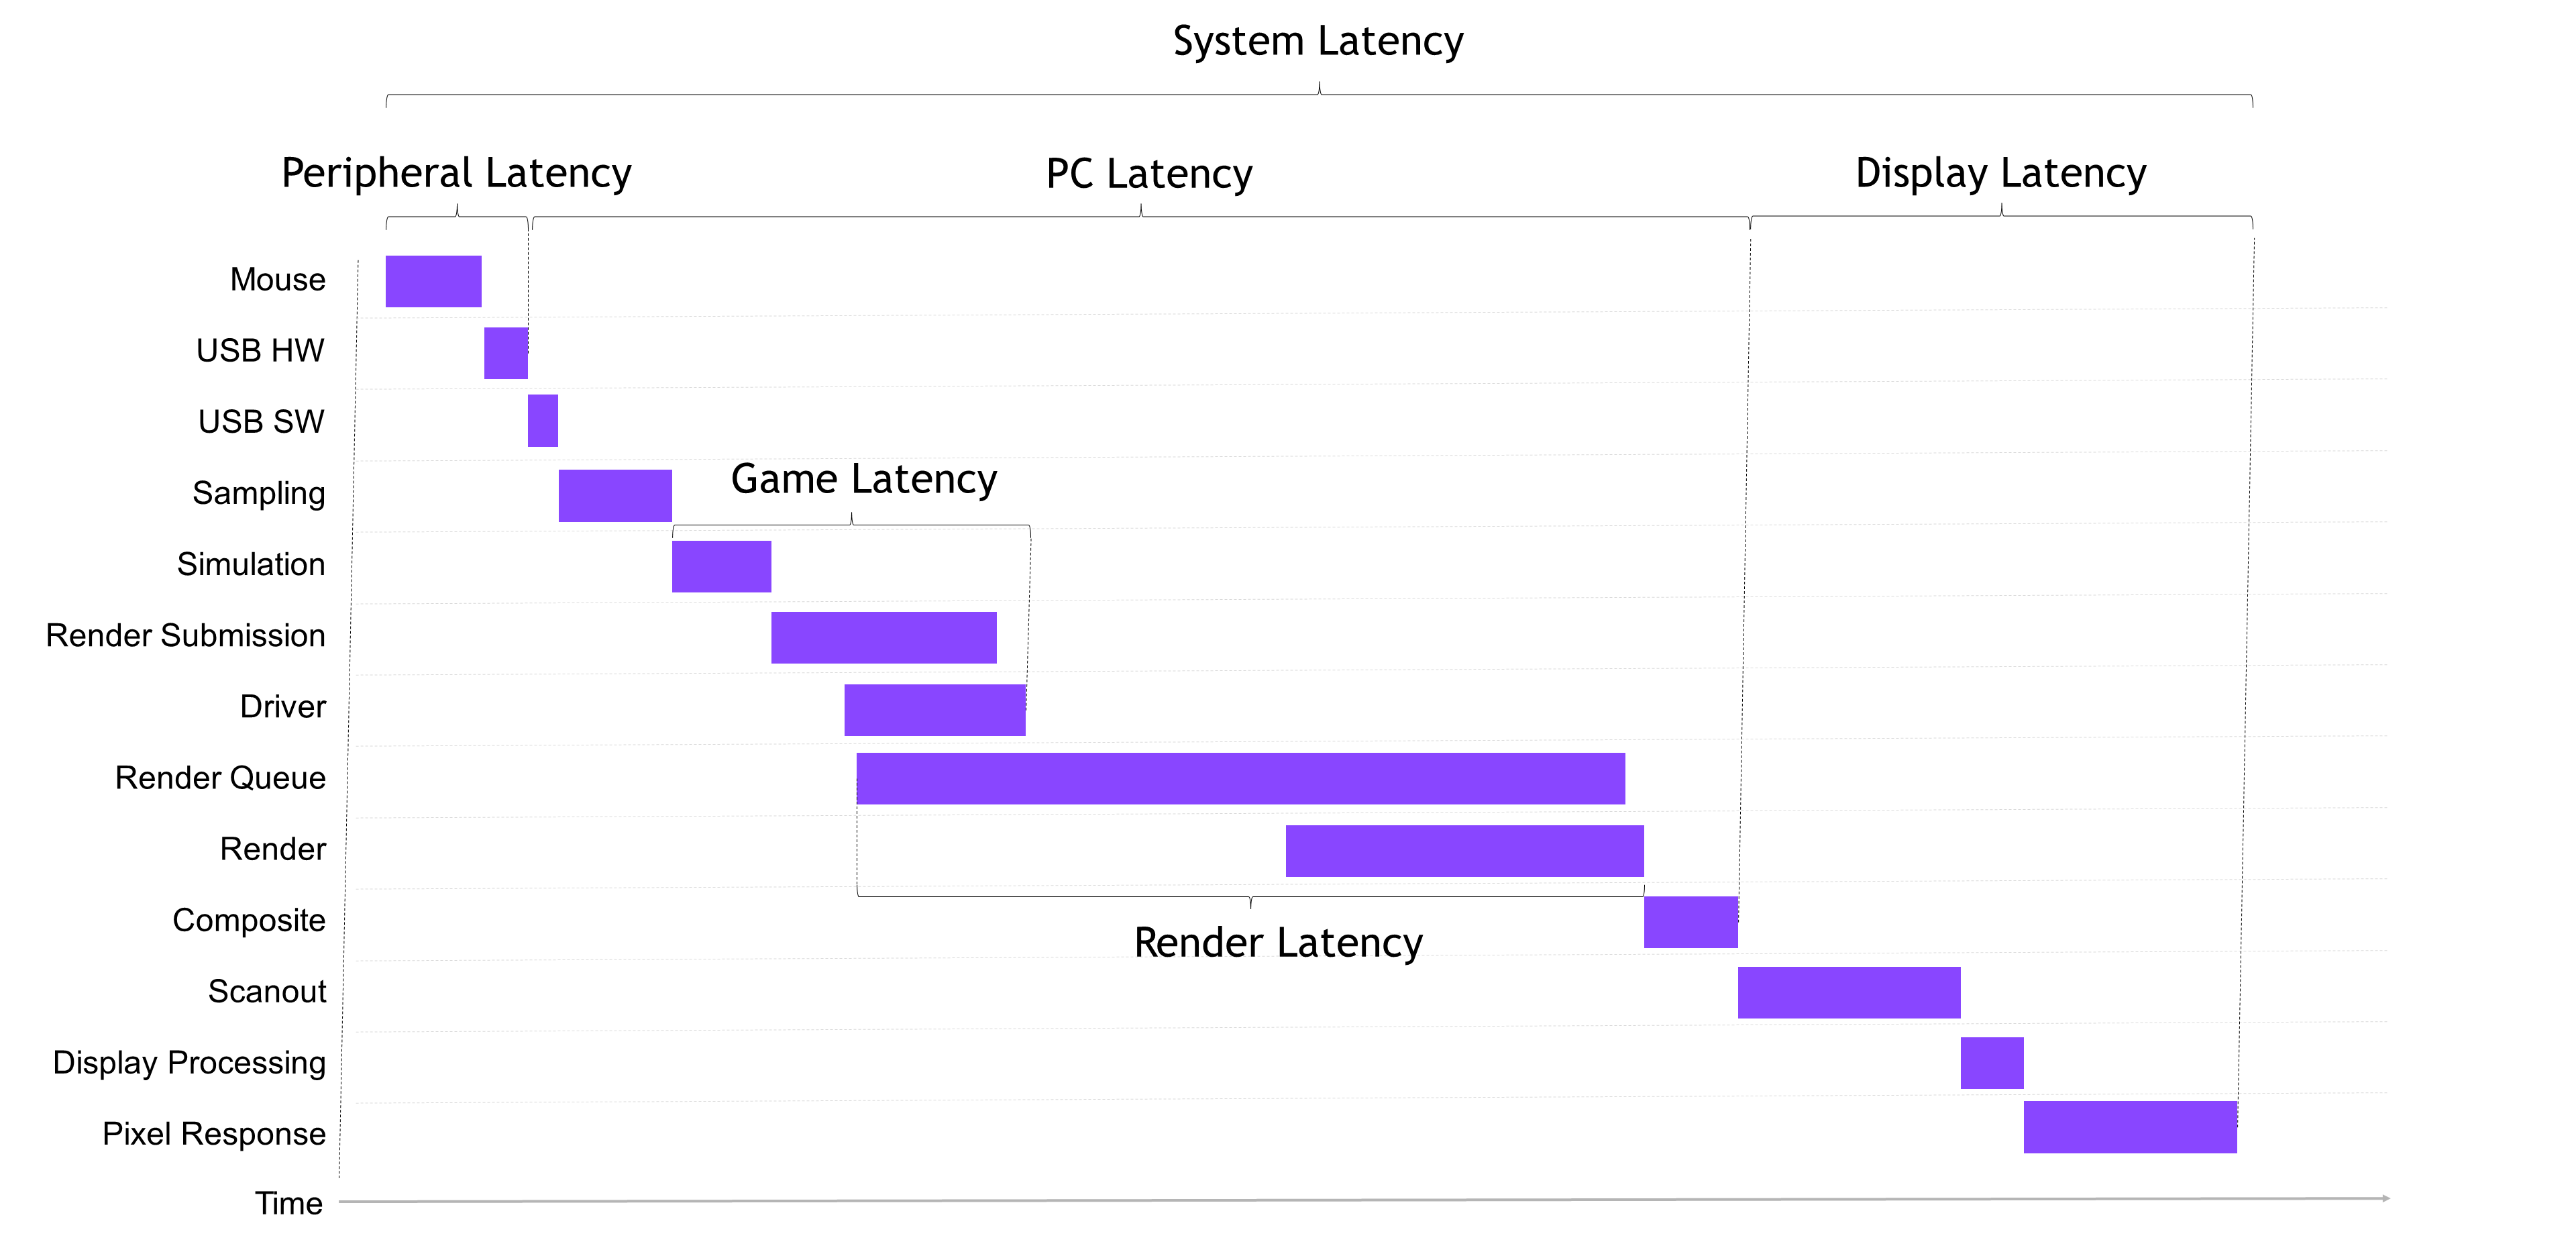
\includegraphics[width=\textwidth]{Introduzione_files/nvidia_latencypipeline.png}
	\caption{Componenti della latenza (dalla documentazione di Nvidia Reflex)}
	\label{fig:nvidia_latencypipeline}
\end{figure}

Nel momento in cui l'utente preme un pulsante sul mouse, l'azione viene registrata dal microcontroller presente all'interno del mouse stesso. Questo microcontroller è responsabile essenzialmente di tre cose:\begin{itemize}
	\item Leggere ripetutamente il sensore ottico per calcolare il movimento
	\item Ricevere le pressioni dei pulsanti sul mouse (ed eseguire il relativo \textit{debouncing})
	\item Memorizzare gli eventi in attesa che il controller USB della macchina a cui è connesso esegua il polling e riceva gli eventi tramite il protocollo USB HID (\textit{Human Interface Device})
\end{itemize}
La velocità con cui avviene il ciclo di lettura dei sensori del mouse è detta \textit{polling rate}, e dipende dalla qualità del mouse stesso. Valori tipici per il \textit{polling rate} sono:
\begin{itemize}
	\item \textbf{125Hz}: la velocità più comunemente usata dai mouse più economici, introduce un ritardo fino a 8ms
	\item \textbf{480Hz}: la velocità tipica dei mouse ``da gaming'' di fascia medio-bassa, introduce un ritardo fino a circa 2ms
	\item \textbf{1000Hz}: la velocità tipica dei mouse di fascia alta, introduce un ritardo fino a 1ms
	\item \textbf{Oltre 1000Hz}: raramente usato da alcuni mouse ``da gaming'' di fascia alta, tenta di ridurre il ritardo a meno di 1ms (ma si applicano considerazioni riguardo al \textit{polling rate} del sistema operativo che saranno discusse successivamente)
\end{itemize}
Quando nelle specifiche di un mouse si parla di \textit{polling rate} o di ritardo di input, il produttore si sta riferendo a questo valore e non deve essere confuso con altri fattori con lo stesso nome.

Attenzione: alcuni mouse, soprattutto quelli senza fili, riducono drasticamente il \textit{polling rate} se restano inattivi per 1-2 secondi.

Periodicamente, il sistema operativo (o il driver del controller USB) eseguono il polling dei dispositivi USB per raccogliere tutti i dati nei loro buffer. La frequenza con cui questa operazione viene eseguita è detta anch'essa \textit{polling rate}, ma non ha nulla a che vedere con il \textit{polling rate} delle specifiche del mouse.\\
Il valore esatto del \textit{polling rate} del sistema operativo dipende dall'hardware sottostante e dalla configurazione del sistema stesso (su Windows, può essere cambiato dal registro di sistema), ma il valore tipicamente usato su hardware di fascia alta è 1000Hz. Il fatto che il sistema esegua il polling a una certa velocità non rende necessariamente inutili i mouse con un \textit{polling rate} più elevato: semplicemente quando viene eseguito il polling, il sistema riceve più di un evento per volta. L'utilizzo di \textit{polling rate} elevati sul mouse è comunque utile per ridurre il \textit{jitter} del movimento (ossia irregolarità nel movimento causate dalla leggera differenza tra il \textit{polling rate} del sistema operativo e quello del mouse, che non sono in alcun modo sincronizzati) e aumentare la velocità massima del movimento che il microcontroller sul mouse stesso è in grado di rilevare prima di perdere precisione.

Attenzione: più è elevato il \textit{polling rate}, sia sul mouse che nel sistema operativo, e più aumenta il numero di eventi che il sistema e le applicazioni devono gestire, e di conseguenza l'uso di CPU. Alcune applicazioni, indipendentemente dalla potenza dell'hardware, non sono in grado di gestire quantità elevate di eventi, e in queste situazioni il ritardo introdotto dal processamento degli eventi supera di gran lunga il ritardo che si avrebbe utilizzando un \textit{polling rate} più basso ma che l'applicazione riesce a gestire correttamente.

A questo punto il sistema operativo ha ricevuto gli eventi dal controller USB e ha il compito di distribuirli alle applicazioni che li ricevono. Tipicamente questo ritardo è trascurabile, a meno di situazioni particolari come un \textit{X11 forwarding} via rete, ma questo è fuori dal contesto di questa tesi. Il metodo di recapito di queste informazioni alle applicazioni può variare in base al tipo di applicazione e di dispositivo di input, ad esempio su Windows un videogioco può ricevere eventi tramite lo stack grafico come qualsiasi altra applicazione, tramite DirectInput, o tramite XInput (per i controller per videogiochi dedicati).

Una volta ricevuti gli eventi, l'applicazione deve gestirli. Questo è uno dei principali fattori che contribuiscono al ritardo di input, e varia enormemente a seconda di come è implementata l'applicazione e dalla velocità dell'hardware sottostante. Un videogioco (o qualsiasi altra applicazione grafica interattiva) tipicamente esegue un loop di questo tipo:
\begin{itemize}
	\item Leggi gli eventi in arrivo dai dispositivi di input
	\item Esegui la logica dell'applicazione (movimento, calcoli dei danni, fisica, AI, caricamenti, eccetera)
	\item Renderizza il fotogramma su un buffer
	\item Presenta il fotogramma sul display
\end{itemize}
In ognuno di questi passaggi, ci possono essere dei ritardi che aumentano il ritardo di input:
\begin{itemize}
	\item Se gli eventi in arrivo sono processati in modo inadeguato dall'engine, potrebbero esserci dei ritardi o una notevole perdita di precisione dei movimenti (ad esempio, se legge un solo evento e scarta tutti gli altri nella coda in arrivo)
	\item Se la logica dell'applicazione richiede molto tempo di CPU per essere eseguita, o applica un qualche tipo di \textit{smoothing} sull'input, questo può introdurre diversi millisecondi di ritardo
	\item Il rendering 3D è solitamente la parte che richiede più tempo: a seconda della complessità della pipeline grafica, dal livello di dettaglio scelto, e dalla potenza dell'hardware sottostante, questo può introdurre severi ritardi: questo è il motivo principale per cui i giocatori professionisti spesso usano hardware molto potente ma giocano con il livello di dettaglio più basso possibile
	\item Il rendering può essere differito, ossia il driver video può ``fingere'' di aver eseguito i comandi che l'applicazione gli ha dato, ma in realtà li ha messi in una coda di rendering che esegue in parallelo ai fotogrammi successivi
	\item A seconda di come è implementata l'applicazione, il fotogramma renderizzato può essere visualizzato in diversi modi.\\
	La tecnica più tipicamente utilizzata è detta \textit{double-buffering}, e consiste nell'avere due buffer della dimensione dello schermo nella memoria della GPU: uno contiene il fotogramma che sta venendo trasmesso correntemente allo schermo, l'altro invece è quello su cui l'applicazione sta renderizzando il fotogramma successivo; quando il rendering è completato, si può:
	\begin{itemize}
		\item Scambiare immediatamente i due buffer e passare al prossimo fotogramma: questo fornisce la latenza migliore, ma crea ``strappi'' nell'immagine che prendono il nome di \textit{tearing}. Questa è la modalità più usata dai giocatori professionisti, ma non tutte le applicazioni sono in grado di gestire \textit{framerate} molto elevati a causa di errori di approssimazione (un esempio famoso è il videogioco del 2011 \textit{``The Elder Scrolls V: Skyrim''}, in cui la fisica è totalmente compromessa da errori di calcolo se il gioco supera i 64 FPS, cosa facilmente riproducibile su qualsiasi PC moderno)
		\item Aspettare l'intervallo di \textit{VBlank} del display, e scambiare i due buffer mentre lo schermo non sta ancora ricevendo il precedente, evitando così il \textit{tearing}: questa tecnica prende il nome di \textit{VSync} (sincronia verticale), e fornisce la qualità dell'immagine migliore a scapito però di un ritardo di input che può aumentare fino a un intero \textit{refresh} del display qualora l'applicazione manchi l'intervallo di \textit{VBlank} di poco. Associata al \textit{double-buffering}, questa tecnica limita il \textit{framerate} dell'applicazione al \textit{refresh rate} del display o ai suoi divisori (ad esempio, per un tipico display a 60Hz, l'applicazione può andare solo a 60, 30, 20, 15, ... FPS)
		\item Se il display supporta un range di \textit{refresh rate} variabile (tipicamente da 48 a 144Hz per i moderni display ``da gaming''), e il \textit{framerate} corrente ricade in quell'intervallo, può inviare immediatamente il nuovo fotogramma al driver della GPU, il quale utilizza la tecnologia VESA Adaptive Sync (o Nvidia G-Sync) per visualizzarlo senza causare \textit{tearing} e senza aumentare il ritardo di input
	\end{itemize}
	Molte applicazioni implementano inoltre, di solito come opzione, il \textit{triplo buffering}. Questa tecnica prevede l'uso di tre buffer della dimensione dello schermo nella memoria della GPU: uno è quello su cui l'applicazione renderizza il fotogramma successivo, uno è quello che l'applicazione vuole visualizzare sullo schermo, e uno è quello che è attualmente visualizzato sullo schermo. Quando il rendering di un fotogramma viene terminato, vengono scambiati i primi due buffer, quando viene raggiunto l'intervallo di \textit{VBlank} del display, vengono scambiati gli ultimi due, ma solo se è stato renderizzato almeno un fotogramma. In questo modo l'applicazione non è più legata al \textit{refresh rate} del display come con il \textit{double-buffering} tradizionale (anche se la maggior parte degli engine limitano comunque il \textit{framerate} al \textit{refresh rate} massimo del display per evitare di sprecare risorse), tuttavia introduce un intero fotogramma in più di latenza, per cui questa tecnica viene usata principalmente quando la qualità dell'immagine è più importante della latenza.
\end{itemize}

Il successivo contributore alla latenza di input è il \textit{compositor} del sistema operativo. Si possono verificare tre scenari principali:
\begin{itemize}
	\item L'applicazione bypassa completamente il \textit{compositor} utilizzando il fullscreen esclusivo e assume il controllo di uno o più display. Questa tecnica è considerata obsoleta, soprattutto perché rende difficile catturare l'output dell'applicazione o visualizzare overlay, ma è ancora usata
	\item L'applicazione chiede al sistema operativo di disattivare il \textit{compositor} mentre è in esecuzione, e crea una finestra senza bordi delle dimensioni dello schermo che vuole riempire. Questo è il caso più comune su GNU/Linux, poiché i \textit{compositor} su questa piattaforma tendono a introdurre problemi di \textit{stuttering}, ma è supportato e usato anche su Windows (da Vista in poi)
	\item L'applicazione passa regolarmente per il \textit{compositor}, creando una finestra senza bordi delle dimensioni dello schermo che vuole riempire Questa modalità introduce una latenza che dipende dal \textit{compositor} utilizzato, ma generalmente è piuttosto elevata
\end{itemize}

Il penultimo fattore che contribuisce alla latenza è il driver della GPU. I driver moderni sono infatti in grado di riconoscere un ampio set di applicazioni, e usano questa informazione per attivare o disattivare alcune funzioni, aggirare dei bug, o semplicemente per migliorare le prestazioni con ottimizzazioni specifiche per l'engine. Tra le varie funzioni che possono essere attivate, quella che introduce il maggior ritardo è la possibilità di permettere all'applicazione di prerenderizzare dei fotogrammi (tipicamente 2, ma fino a 10 nel driver di Nvidia per Windows). Dal punto di vista dell'applicazione, quei fotogrammi è come se fossero stati mandati al display, ma in realtà il driver li mette in una coda di fotogrammi che manda avanti a intervalli regolari. Questa tecnica permette di ridurre drasticamente lo \textit{stuttering} presente in molti giochi moderni causato da \textit{texture streaming}, \textit{level streaming}, \textit{garbage collection}, eccetera, migliorando così la fluidità del video, a scapito però di un elevatissimo costo in termini di latenza. Il rendering stesso dei fotogrammi può essere messo in una coda di rendering ed essere eseguito più tardi senza che l'applicazione lo sappia, riducendo il carico sull'applicazione. I driver di AMD e Nvidia offrono entrambi una modalità a bassa latenza che disattiva la prerenderizzazione dei fotogrammi, attivata di default per alcune applicazioni a latenza critica. Nvidia offre inoltre, per alcune applicazioni di cui è in grado di predire i tempi di elaborazione e rendering, la possibilità di inserire un ritardo strategico prima che gli eventi in input vengano letti; questo permette di far si che il maggior numero di eventi venga processato prima che l'applicazione si metta ad attendere il \textit{VBlank}, riducendo così la latenza di alcuni millisecondi quando il \textit{VSync} è attivo.

L'ultima causa di latenza, nonché uno dei principali contributori, è il display stesso. A differenza dei vecchi monitor CRT in cui i segnali generati dalla scheda video andavano a pilotare direttamente, tramite la connessione VGA analogica, il fascio di elettroni che disegna l'immagine, risultando in una latenza nulla, i moderni display LCD hanno un'interfaccia digitale che richiede una notevole elaborazione all'interno del display stesso.\\
Quando l'immagine arriva al display, viene memorizzata in un buffer su cui il processore all'interno del monitor può eseguire alcune elaborazioni, come lo \textit{scaling}, l'applicazione di filtri, eccetera. Sui monitor per PC tipicamente questo ha un ritardo di un fotogramma (per alcuni display anche meno, come vedremo nel capitolo sui risultati sperimentali); i televisori invece tendono a memorizzare più fotogrammi per eseguire elaborazioni più sofisticate, come l'interpolazione del movimento, aumentando notevolmente il ritardo di input, ma a volte forniscono una ``modalità gioco'' che disattiva queste funzioni, facendolo comportare come un monitor normale. Il ritardo di processamento all'interno del monitor è chiamato a volte \textit{``input lag''} (ritardo di input) nelle specifiche del monitor, ma è riferito al display stesso, non all'intero sistema, ed è importante non fare confusione.\\
Una volta eseguite tutte le elaborazioni necessarie, il processore nel display ha il compito di comandare il pannello LCD per visualizzare l'immagine. Il modo in cui questo avviene dipende dalla tecnologia utilizzata; il \textit{refresh} dell'intero pannello avviene solitamente dall'alto verso il basso e richiede alcuni millisecondi per essere completato (tipicamente la metà del tempo di un fotogramma); il tempo necessario affinché i pixel cambino colore è detto tempo di risposta dei pixel, ed è l'ultimo passo del percorso; tipicamente è nell'ordine di 5-10 millisecondi (nonostante i produttori spesso dichiarino tempi di 1ms o meno, questo avviene solo in condizioni particolari), ma varia molto a seconda della tecnologia utilizzata e della qualità del display stesso.

Il processo è ora terminato e l'utente può vedere l'immagine sul display; questo conclude questa sezione sui fattori chiave del ritardo di input.

\section{Funzionamento di un display}
Questa sezione introduce il funzionamento di alcuni tipi di display moderni. Non è in alcun modo esaustiva, ma è utile conoscere le basi del funzionamento prima di continuare nei capitoli successivi.

Nel corso dei decenni, sono stati sviluppati innumerevoli tipi di display, ma le tecnologie più comunemente usate oggi sono LCD TFT e OLED: i primi sono più comuni sui PC, mentre i secondi si trovano prevalentemente sugli smartphone e i televisori.\\
Una differenza fondamentale tra un display OLED e un LCD TFT, è che i primi non hanno bisogno di retroilluminazione, poiché i pixel stessi emettono luce, mentre i secondi hanno bisogno di un qualche tipo di retroilluminazione poiché si basano su filtri che bloccano o lasciano passare la luce della retroilluminazione.\\
La retroilluminazione di un display LCD può essere realizzata in diversi modi: tradizionalmente si utilizzavano dei tubi a fluorescenza (CCFL) posizionati sui lati del display che illuminano un diffusore bianco generando una retroilluminazione più o meno uniforme; i tubi CCFL sono stati poi sostituiti da dei LED bianchi, posizionati sempre sui lati ad illuminare un diffusore; più recentemente i display di fascia alta hanno iniziato ad adottare un array di LED bianchi posizionati dietro al diffusore anziché sui lati, spesso individualmente controllabili per fornire un migliore contrasto (\textit{Full Array Local Dimming}\cite{localdimming}).\\
Con l'introduzione dei LED nella retroilluminazione, ci si scontra con il problema del dimming dei LED stessi: per simulare livelli bassi di luminosità, molti display, soprattutto quelli più economici, usano la tecnica della PWM (\textit{Pulse Width Modulation}\cite{pwm_backlight}) per accendere e spegnere molto velocemente i LED creando l'illusione all'occhio umano di valori intermedi di luminosità. La frequenza più comune per la PWM è 240Hz, ma non è l'unica. Display di fascia più alta invece sono in grado di controllare il livello di luminosità dei LED in tensione o in corrente grazie a della circuiteria più sofisticata ma più costosa.

Davanti alla retroilluminazione, nei display LCD TFT, è presente una struttura che ha il compito di far passare o bloccare la luce alterando lo stato di uno strato di cristalli liquidi. Esistono principalmente tre tecnologie per fare questo, ognuna con i suoi vantaggi e svantaggi:
\begin{itemize}
	\item TN (\textit{Twisted Nematic}): due filtri polarizzati di vetro sono posizionati rispettivamente dietro e davanti ad uno strato di cristalli liquidi, con una rotazione di 90°. Applicando una tensione allo strato di cristalli liquidi, si riesce ad alterarne la struttura in modo da variare la polarizzazione della luce che vi passa attraverso. A seconda della tensione applicata, passerà più o meno luce. Questo tipo di tecnologia è ancora oggi ampiamente utilizzata, soprattutto dai giocatori, per i bassi tempi di risposta, ma fornisce le peggiori prestazioni in termini di angolo di visione e qualità dell'immagine\cite{tftcentral_paneltech}
	\item IPS (\textit{In-Plane Switching}): a differenza dei display TN, i due filtri polarizzati sono paralleli e non ruotati di 90°. Per ottenere la rotazione di 90° del cristallo liquido, le parti interne del vetro dei due filtri sono trattate per allineare le molecole esterne del cristallo liquido alla giusta angolazione. Applicando una tensione con due elettrodi posizionati entrambi sullo stesso piano, si fa scorrere una corrente nel cristallo liquido essenzialmente parallela al piano, e si crea la rotazione che blocca o fa passare la luce. Questo è il tipo di tecnologia più utilizzata al momento, e fornisce la miglior qualità dell'immagine e angoli di visione, a scapito però di tempi di risposta relativamente alti, un maggior consumo di energia, costi più elevati, un nero poco profondo, e spesso una scarsa uniformità della retroilluminazione (detta \textit{backlight bleeding})\cite{tftcentral_paneltech}
	\item VA (\textit{Vertical Alignment}): simile a TN, ma i cristalli liquidi si allineano naturalmente in modo verticale ai filtri, bloccando il passaggio della luce. Applicando una tensione al cristallo liquido, questo si ruota verticalmente, permettendo a più o meno luce di passare in base alla tensione. Questa tecnologia è meno comune rispetto a IPS e TN, fornisce il miglior contrasto tra le tre, buoni tempi di risposta, e una qualità dell'immagine molto buona, seppur non ai livelli di un IPS; sfortunatamente è anche quella con l'angolo di visione più stretto\cite{mva1}\cite{tftcentral_paneltech}, così stretto che una sorta di effetto tunnel sui bordi è pienamente visibile anche alla distanza e angolazione di utilizzo normale, motivo per cui è poco utilizzata
\end{itemize}

Dopo aver attraversato il cristallo liquido, la luce viene colorata da uno strato di filtri colorati detto maschera (\textit{mask}) che contiene la matrice RGB che compone i pixel dello schermo.

Per controllare l'applicazione di tensione al cristallo liquido, delle linee di controllo verticale e orizzontale sono posizionate a matrice tra i pixel e permettono di controllare un TFT (Thin Film Transistor) presente in ogni \textit{subpixel}. Questi piccolissimi transistor sono utilizzati per applicare la tensione al cristallo liquido\cite{lcdevolution}.\\
I \textit{subpixel} non sono indirizzabili individualmente (sarebbero necessarie troppe connessioni), il loro stato viene tipicamente aggiornato una linea per volta, ed è compito della matrice mantenere questo stato fino al \textit{refresh} successivo usando un condensatore assieme al transistor per mantenere l'informazione mentre le altre linee vengono aggiornate. Questa tecnica prende il nome di \textit{active matrix}\cite{lcdevolution} (matrice attiva), e tutti i display TFT moderni usano questo tipo di matrice.

Alcuni display, soprattutto quelli più economici, non utilizzano tutta l'informazione presente nell'immagine in arrivo dalla scheda video per controllare i \textit{subpixel} (ad esempio, su 8 bit per canale potrebbero usarne solo 6), così da avere una circuiteria più semplice e meno costosa, e compensano facendo uso di tecniche di \textit{dithering} spaziale e/o temporale.

\begin{figure}[h]
	\centering
	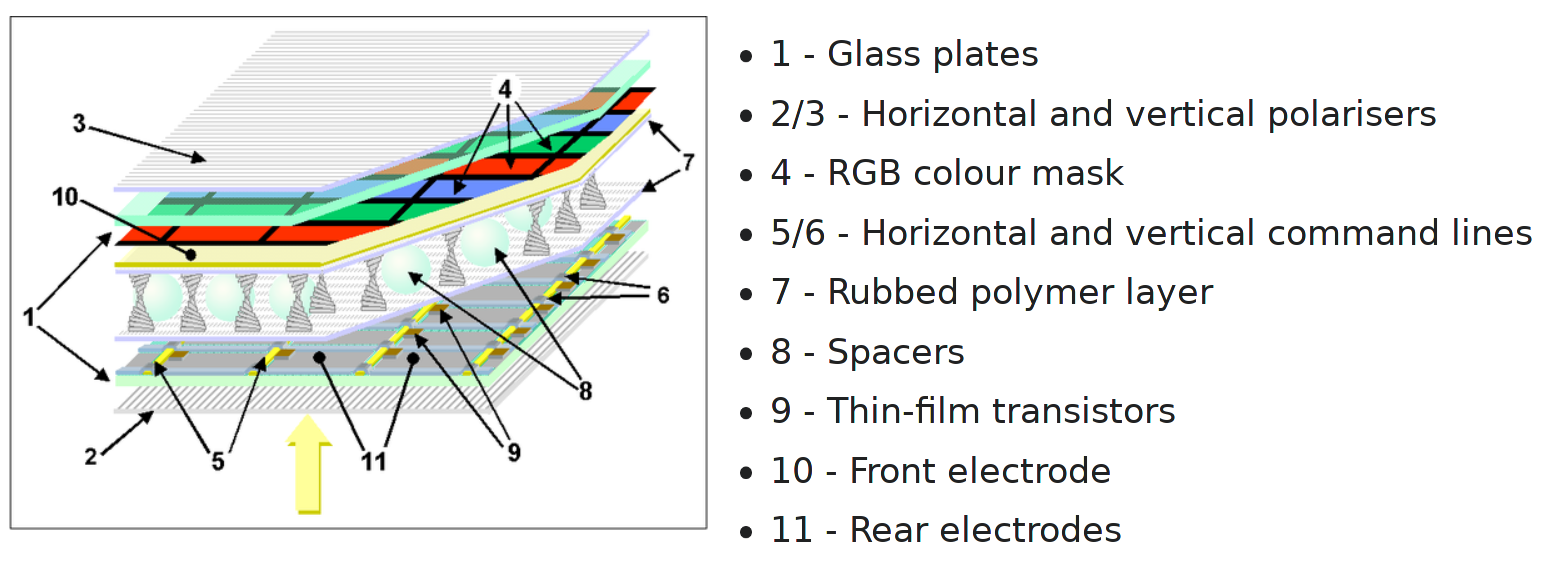
\includegraphics[width=\textwidth]{Introduzione_files/lcdtft.png}
	\caption{Struttura di un display LCD TFT (da Wikipedia, l'enciclopedia libera)}
	\label{fig:lcdtft}
\end{figure}

Per quanto riguarda i display OLED, le cose sono un po' più semplici: si tratta sostanzialmente di una matrice di piccolissimi LED organici controllati da una matrice attiva\cite{amoled1}. Ogni LED è composto da due elettrodi, uno dei quali è trasparente, e nel mezzo è presente un polimero organico che emette luce quando viene applicata una tensione. Non richiedono retroilluminazione poiché i LED emettono luce propria anziché filtrarla, il che permette di creare display trasparenti con una buona visibilità, display flessibili\cite{flexibleoleds}, display estremamente sottili (ragione per cui sono comuni sugli smartphone). Il contrasto è eccezionale e i tempi di risposta sono buoni, tuttavia si usurano molto più velocemente rispetto ai display LCD TFT, anche se inutilizzati, l'usura non è uniforme nè nello spazio nè nei colori, soffrono di \textit{burn-in} (ossia immagini statiche come loghi visualizzate a lungo restano impresse permanentemente sul display), e il polimero organico è estremamente vulnerabile ai liquidi e all'umidità.

\begin{figure}[h]
	\centering
	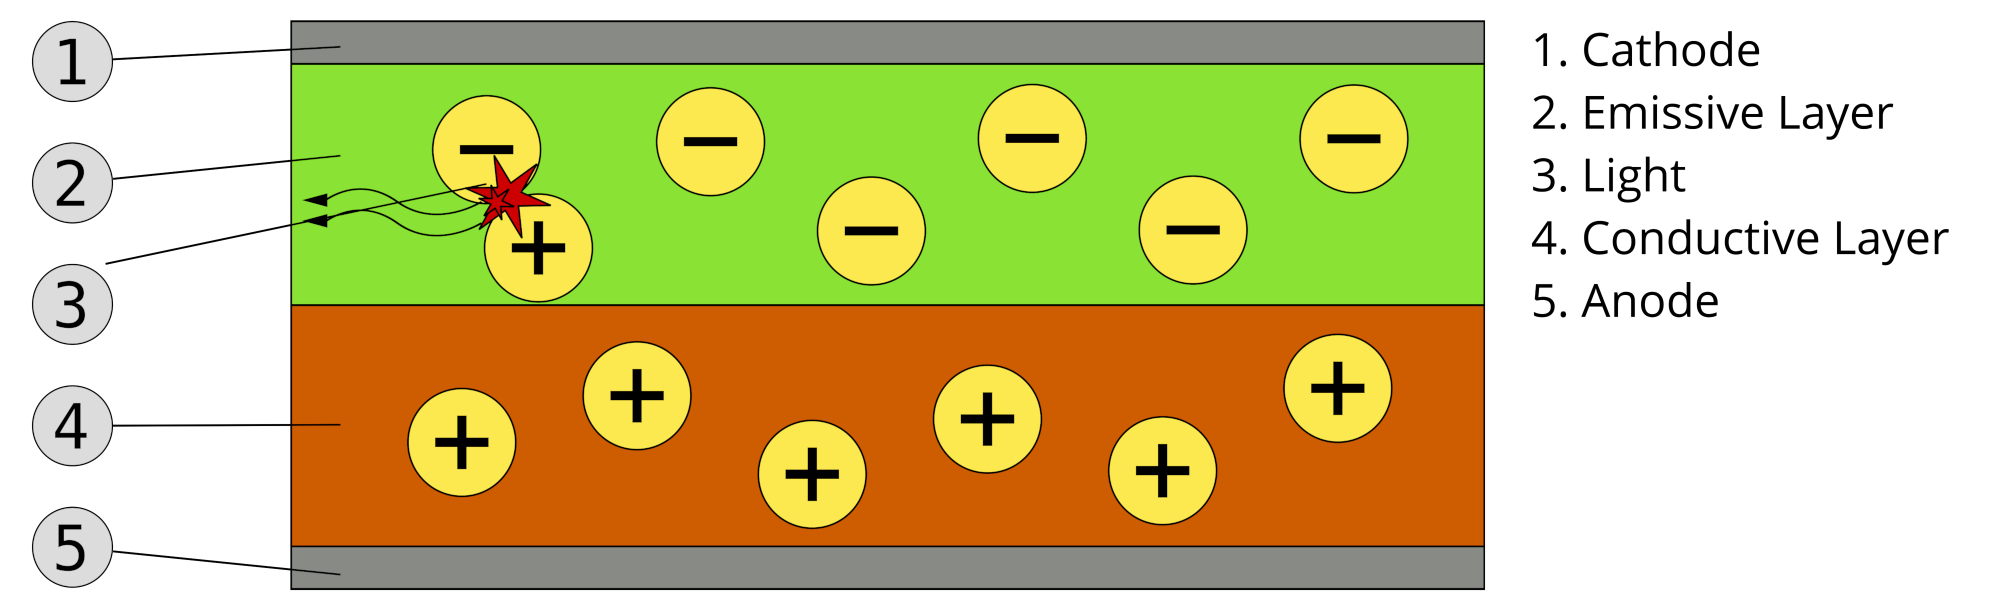
\includegraphics[width=\textwidth]{Introduzione_files/oled.png}
	\caption{Struttura di un \textit{subpixel} OLED (da Wikipedia, l'enciclopedia libera)}
	\label{fig:oled}
\end{figure}

Il passo finale nella produzione del display è uno strato protettivo di vetro per proteggere il tutto. Questo vetro può essere lucido per esaltare i colori, oppure avere una grana molto fine, per ridurre i riflessi.

Questo conclude la panoramica sulle tecnologie di display più comunemente utilizzate.

\section{Il progetto OpenLDAT}
\subsection{Storia del progetto}
L'idea del progetto OpenLDAT nasce intorno a Marzo 2019, quando durante una presentazione di Google Stadia, discutendo i problemi di latenza dell'idea di eseguire videogiochi in streaming, viene mostrata al pubblico la tabella in figura \ref{fig:stadialies}.
\begin{figure}[h]
	\centering
	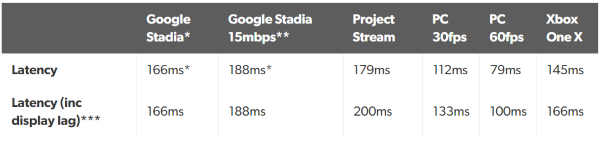
\includegraphics[width=\textwidth]{Introduzione_files/lies.png}
	\caption{Latenze secondo Google}
	\label{fig:stadialies}
\end{figure}

Ignorando per un momento il fatto che, secondo Google, Stadia ha lo stesso ritardo di input indipendentemente dal display utilizzato, che è impossibile, i numeri mostrati attirano subito l'attenzione di qualsiasi giocatore esperto, soprattutto su PC, poiché sembrano alquanto elevati. Sebbene sia vero che alcuni giochi, soprattutto quelli basati sulla storia che non richiedono di eseguire azioni rapide, hanno un ritardo elevato per migliorare la consistenza dei tempi dei fotogrammi, non è sicuramente rappresentativo nè del caso medio, nè del caso in cui la latenza è critica, come nei giochi musicali.

Vedendo questi dati, è stato deciso di costruire un semplice dispositivo per verificarli. Il dispositivo creato utilizzava un microcontroller per simulare la pressione di un tasto, la quale veniva ricevuta da un'applicazione OpenGL che generava un flash sullo schermo, che veniva rilevato da un fotoresistore collegato al microcontroller, il quale poi inviava via seriale il tempo trascorso tra l'invio del segnale e la ricezione del flash. La procedura veniva ripetuta 10 volte per avere un valore medio più accurato.

Eseguendo il test era stato ottenuto un ritardo medio di circa 50ms\cite{fdossena1}, su un display non ``da gaming''. Questo è rappresentativo del ritardo che subirebbe un videogioco programmato per avere una buona latenza sulla configurazione su cui era stato testato. Successivi test con un display a bassa latenza hanno abbassato la misura a circa 20ms.

Questa prima versione del progetto non è mai stata rilasciata per via di alcune limitazioni:
\begin{itemize}
	\item Il sensore utilizzato (un semplice fotoresistore) è relativamente lento\cite{adafruit_photores}, con un tempo di risposta di diversi millisecondi sia in salita che in discesa, il che significa che, senza un'accurata calibrazione, i risultati potrebbero essere seriamente sovrastimati
	\item Non c'era modo di regolare la soglia di attivazione del sensore se non variando delle resistenze (il sensore generava un interrupt)
	\item Il software non era in grado di gestire alcun tipo di disturbo nel segnale in arrivo dal sensore, il che causava risultati totalmente errati se veniva usato su display con retroilluminazione PWM, o dei vecchi CRT
	\item Il test funzionava solo in presenza dei flash sullo schermo, quindi non era possibile testare le diverse latenze di diverse applicazioni con questo metodo
\end{itemize}

A Novembre 2019, il lancio di Google Stadia ha attirato l'attenzione dei giornalisti del settore, i quali hanno cercato di eseguire un esperimento simile\cite{gamersnexus_stadia} \cite{gamersnexus_stadia2}, utilizzando un mouse modificato per accendere un LED quando viene premuto un tasto, e una telecamera ad alta velocità per misurare (con una risoluzione di qualche millisecondo) il tempo trascorso tra l'accensione del LED e l'inizio dell'azione sul display. L'utilizzo di metodi così ``crudi'' e manuali, anche da parte della stampa più tecnica e professionista evidenzia l'assenza di dispositivi per una facile analisi delle metriche di latenza dei display. Circa 2 anni dopo il lancio di Stadia, Google ha effettivamente raggiunto alcuni dei numeri promessi nella presentazione di Marzo 2019, ma al lancio l'opinione generale è stata pessima.

A Settembre 2020, Nvidia ha inviato un prototipo di un dispositivo chiamato Nvidia LDAT (Latency Display Analysis Tool) a diversi giornalisti del settore\cite{gamersnexus_nvidialdat}, un dispositivo quasi del tutto analogo a quello descritto in precedenza, ma con un sensore e un software migliori. Vedere questo progetto in azione ha fornito lo stimolo a far ripartire il progetto, che è poi stato realizzato nei mesi successivi. Sfortunatamente Nvidia ha deciso di non commercializzare il dispositivo, per cui si conosce poco dei dettagli sul funzionamento, ma verrà comunque discusso nel capitolo successivo sullo stato dell'arte.

Nel periodo tra Dicembre 2020 e Marzo 2021 è stato svolto gran parte del lavoro sul progetto OpenLDAT che, assieme ai dati sperimentali, è oggetto di questa tesi.

Nel periodo tra Marzo 2021 e Giugno 2021 è stata scritta questa tesi, sono stati eseguiti test su vari tipi di display, e sono state fatte migliorie agli algoritmi per assicurarne il buon funzionamento sul maggior numero possibile di display.

\subsection{Obiettivi del progetto}
Il progetto OpenLDAT si pone i seguenti obiettivi principali:
\begin{itemize}
	\item Fornire agli utenti un dispositivo per poter misurare, sia automaticamente che interattivamente, la latenza totale del proprio sistema, nel modo più accurato possibile, e permettendo il confronto tra sistemi e scenari diversi
	\item Rendere il dispositivo utilizzabile sul maggior numero possibile di display, anche in presenza forti disturbi come una retroilluminazione PWM
	\item Utilizzare il sensore nel dispositivo per fornire ulteriori metriche che non riguardano esclusivamente la latenza, ma anche la qualità del display, come una stima dei tempi di risposta reali dei pixel in diversi scenari
	\item Rendere il dispositivo facilmente costruibile, utilizzando componenti \textit{off-the-shelf}, facilmente reperibili, dai costi contenuti, e un software che non richieda calibrazioni
	\item Distribuire tutte le schematiche del dispositivo e il software su licenza libera, per consentire agli utenti di capirne il funzionamento e potenzialmente anche di apportare migliorie
\end{itemize}

Inizialmente, il progetto è rivolto principalmente a un pubblico tecnico, poiché è necessario sapersi assemblare il dispositivo da sè; qualora ci fosse interesse sufficiente per il progetto, però, diventerebbe possibile distribuirlo come prodotto finito e pronto all'uso; in questo caso il target si espanderebbe notevolmente, e diventerebbe usufruibile anche a un pubblico di giornalisti di tecnologia se non addirittura potenziali acquirenti in cerca di un nuovo monitor.

\subsection{Struttura del repository del progetto}
Tutti i file relativi al progetto OpenLDAT sono disponibili sul relativo repository GitHub\footnote{\url{https://github.com/adolfintel/OpenLDAT}}. %è privato fino a fine tesi

Il respository è strutturato in questo modo:\begin{itemize}
	\item \texttt{App}: contiene il codice dell'applicazione OpenLDAT per PC e i file necessari per creare i \textit{package} distribuibili. \begin{itemize}
		\item \texttt{OpenLDAT}: progetto dell'applicazione per NetBeans
		\item \texttt{Packaging stuff}: file necessari per creare i \textit{package} distribuibili per Windows, GNU/Linux e MacOS
	\end{itemize}
	\item \texttt{Device}: contiene tutti i file relativi al dispositivo fisico OpenLDAT: \begin{itemize}
		\item \texttt{Case}: modelli 3D per il case stampabile e relative istruzioni
		\item \texttt{Firmware}: file relativi al firmware del dispositivo \begin{itemize}
			\item \texttt{OpenLDAT}: progetto del firmware per Arduino IDE
			\item \texttt{boards.txt}: dichiarazione del dispositivo per Arduino IDE
			\item \texttt{Libraries.zip}: copia di backup delle librerie necessarie per compilare il firmware, qualora non fossero più disponibili in futuro
			\item \texttt{Prebuilt}: firmware precompilato per programmare il dispositivo senza Arduino IDE
		\end{itemize}
		\item \texttt{Hardware}: file relativi al circuito del dispositivo: \begin{itemize}
			\item \texttt{OpenLDAT\_Model1.fzz}: progetto del dispositivo per Fritzing
			\item \texttt{gerber}: file del PCB del dispositivo in formato standard gerber per la stampa
		\end{itemize}
	\end{itemize}
	\item \texttt{Docs}: documentazione del dispositivo e dell'applicazione, in inglese
\end{itemize}

Questo conclude il capitolo introduttivo. Nei capitoli successivi verrà discusso lo stato dell'arte, confrontando OpenLDAT con progetti, dopodiché verrà introdotto il dispositivo stesso.


\newpage
\setlength{\parskip}{10pt}
\setlength{\parindent}{0pt}
\chapter{Stato dell'arte}
\label{chap:statoarte}

In questo capitolo vengono introdotti alcuni progetti già esistenti che sono in qualche modo simili o correlati al progetto OpenLDAT, e in che modo differiscono da esso. Sono stati scelti a titolo esemplificativo Nvidia LDAT, DisplayCAL e il dispositivo di RTINGS usato per le loro recensioni, ma questo non è in alcun modo un elenco esaustivo. Poiché Nvidia LDAT è il progetto più simile, nel capitolo \ref{chap:outro} verrà mostrata una tabella comparativa tra Nvidia LDAT e OpenLDAT.

\section{Nvidia LDAT}
Intorno al mese di Settembre 2020, Nvidia ha distribuito un prototipo di un dispositivo chiamato Nvidia LDAT, abbreviazione di Latency Display Analysis Tool. Questo dispositivo, che non è stato poi commercializzato, è stato una delle maggiori ispirazioni per il progetto OpenLDAT.

Il dispositivo Nvidia LDAT si presenta come una piccola scatola di plastica stampata in 3D su cui sono presenti un LED RGB che indica lo stato del dispositivo e i click, un sensore di luminosità, una porta Micro-USB per collegarlo ad un PC che esegue il software di LDAT, un connettore per un mouse modificato, una corda per poterlo appendere più facilmente al display, e un jack audio che può essere opzionalmente collegato dalla macchina di test al dispositivo. La figura \ref{fig:nvldat_front} mostra la parte frontale del dispositivo.

\begin{figure}[h!]
	\centering
	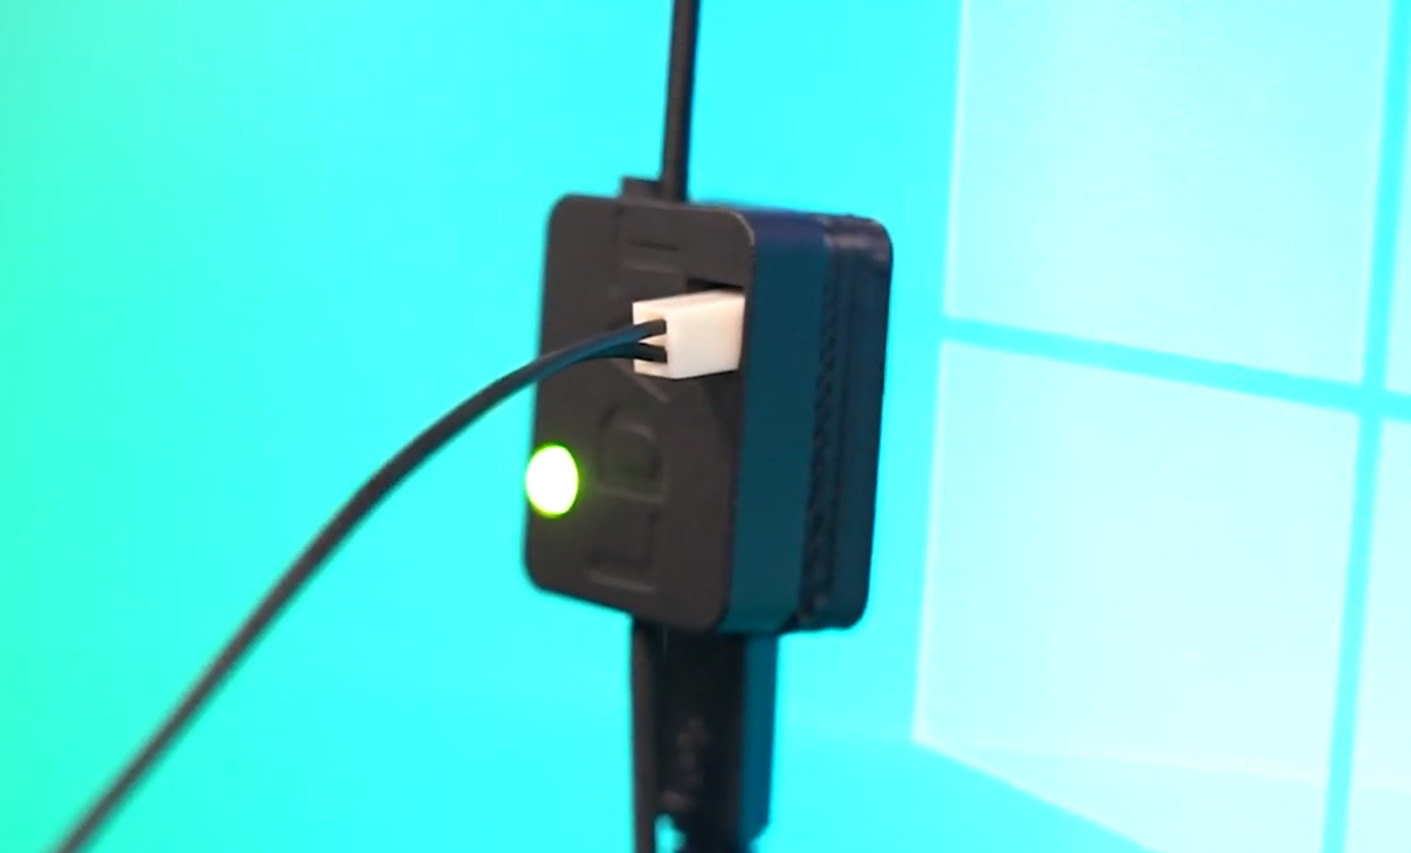
\includegraphics[width=0.8\textwidth]{StatoDellArte_files/nvldat_front.jpg}
	\caption{Parte frontale del dispositivo Nvidia LDAT (da GamersNexus)}
	\label{fig:nvldat_front}
\end{figure}

Non è noto nulla riguardo all'hardware presente all'interno, ma dall'immagine in figura \ref{fig:nvldat_back}, il sensore di luminosità sembra essere un fotodiodo piuttosto grande, o forse addirittura un CCD. Non sono stati eseguiti dei \textit{teardown} del dispositivo, probabilmente su esplicita richiesta di Nvidia, per cui non è stato possibile osservare il tipo di microcontroller o l'elettronica all'interno.

\begin{figure}[h!]
	\centering
	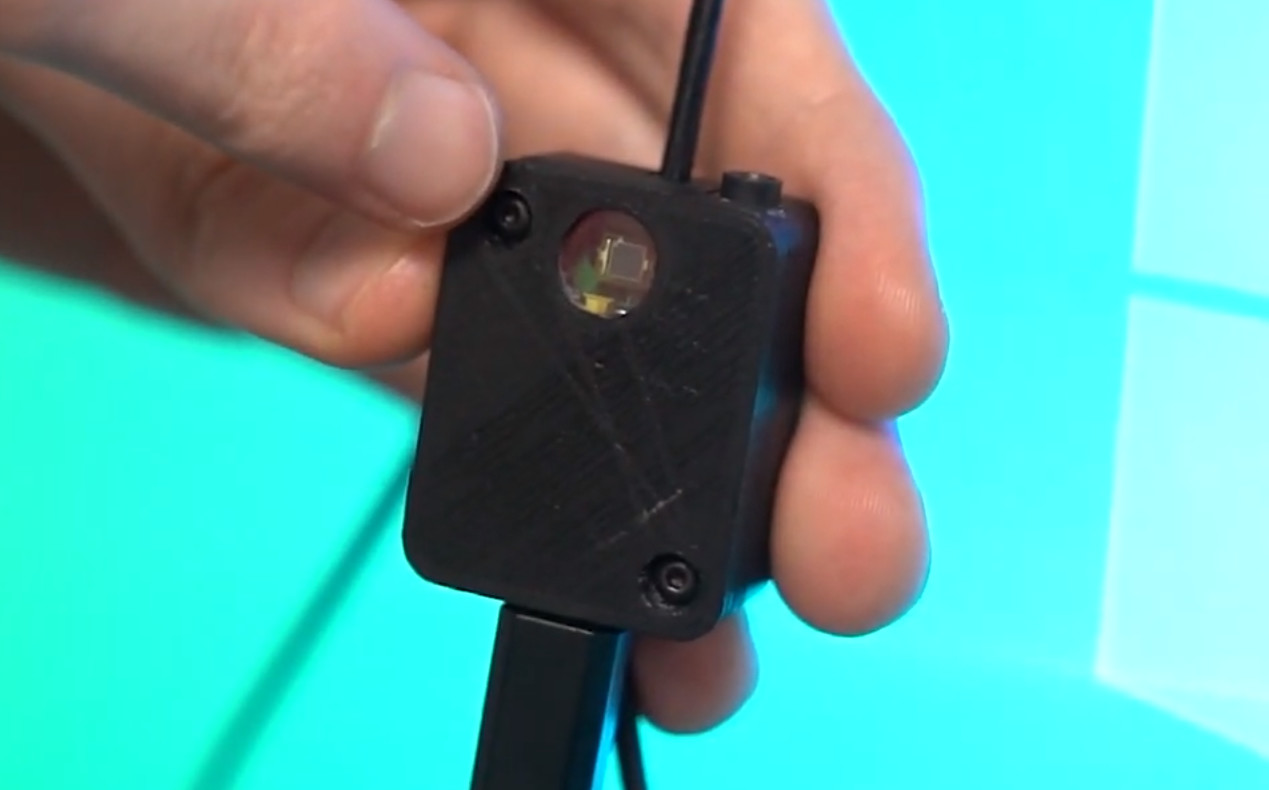
\includegraphics[width=0.8\textwidth]{StatoDellArte_files/nvldat_back.jpg}
	\caption{Parte posteriore del dispositivo Nvidia LDAT (da GamersNexus)}
	\label{fig:nvldat_back}
\end{figure}

Il software di Nvidia LDAT implementa un test per misurare quella che Nvidia chiama \textit{click-to-photon response}, ossia il tempo che passa tra la pressione di un click del mouse e il cambio di luminosità sullo schermo. Il test può essere eseguito in modo automatico, con il dispositivo che esegue i click su un'applicazione, oppure in modo manuale, utilizzando un mouse modificato collegato ai due pin sulla parte frontale del dispositivo.\\
Il software fornisce inoltre la possibilità di misurare il ritardo utilizzando l'audio catturato tramite il jack presente sul dispositivo. Questa scelta è piuttosto bizzarra, poiché la scheda audio ha una latenza diversa rispetto allo stack grafico e il display, ma può comunque fornire una stima del ritardo poiché le applicazioni processano gli input a intervalli regolari che dipendono dal framerate, per cui un'applicazione a 30 FPS avrà più ritardo di una a 60 FPS, anche sull'audio.\\
La figura \ref{fig:nvldat_software} mostra uno screenshot del software Nvidia LDAT in azione.

\begin{figure}[h!]
	\centering
	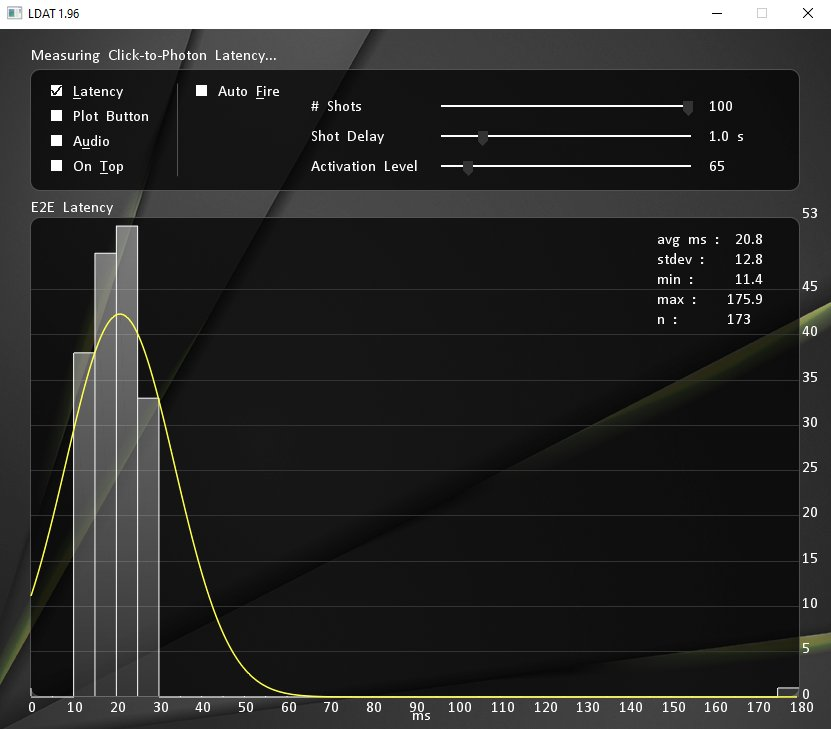
\includegraphics[width=0.8\textwidth]{StatoDellArte_files/nvldat_software.jpg}
	\caption{Screenshot del software Nvidia LDAT (da igorslab.de)}
	\label{fig:nvldat_software}
\end{figure}

Il dispositivo è stato aggiornato intorno a Maggio 2021, con un case di plastica non stampata e l'aggiunta di un pulsante sulla parte frontale del dispositivo per interagire con il software Nvidia LDAT mentre il dispositivo esegue i test e la possibilità di collegare un sensore di luminosità esterno. Per il resto, il dispositivo sembra invariato. La figura \ref{fig:nvldat_v2} mostra il nuovo case.

\begin{figure}[h!]
	\centering
	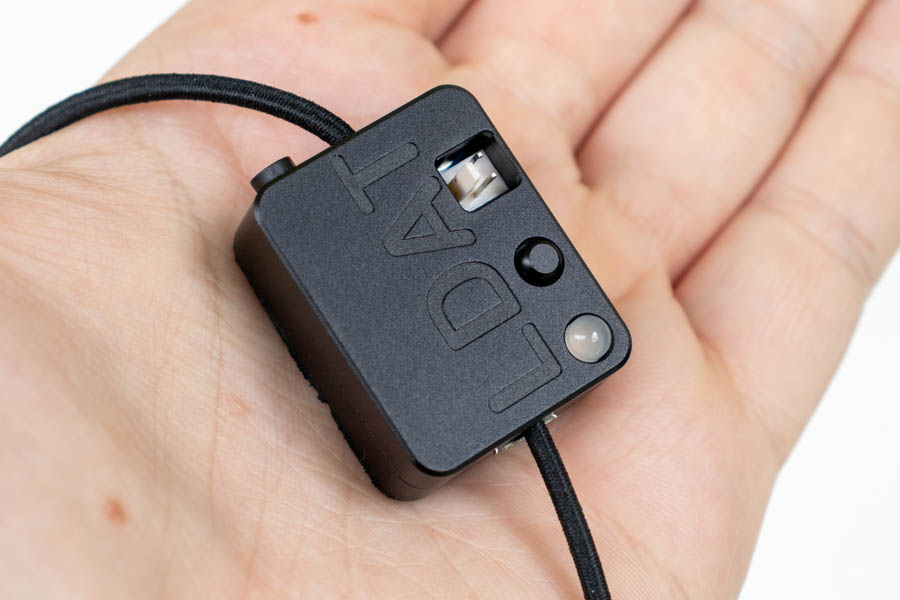
\includegraphics[width=0.8\textwidth]{StatoDellArte_files/nvldat_v2.jpg}
	\caption{Nuova versione di Nvidia LDAT (da techpowerup.com)}
	\label{fig:nvldat_v2}
\end{figure}

Nvidia purtroppo ha scelto di non commercializzare nessuna versione di questo dispositivo, ma lo ha solo distribuito ad alcuni giornalisti di tecnologia come parte di un \textit{``reviewers kit''}, ma ha creato Nvidia Reflex Latency Analyzer, una sorta di versione \textit{built-in} in alcuni monitor e mouse compatibili che è in grado di misurare la latenza senza bisogno di dispositivi esterni.

Nvidia Reflex Latency Analyzer\footnote{\url{https://www.nvidia.com/en-us/geforce/news/reflex-latency-analyzer-360hz-g-sync-monitors/}} consente ai display con certificazione G-Sync Ultimate (ossia con un processore Nvidia dedicato al loro interno) di eseguire il lavoro che normalmente svolgerebbe il sensore di luminosità, monitorando una piccola area dell'immagine per rilevare variazioni di luminosità. Un mouse compatibile deve essere collegato al display stesso, e il software sarà in grado di misurare il ritardo dell'intero sistema.\\
Il requisito di un mouse esplicitamente supportato da Nvidia è necessaria al software per poter conoscere quanto del ritardo è causato dal mouse stesso e quanto dal resto del sistema. Il tempo di latenza calcolato da questo sistema è sostanzialmente lo stesso che verrebbe misurato con un dispositivo esterno come Nvidia LDAT, a meno di pochi millisecondi dovuti al tempo di risposta dei pixel del display. La figura \ref{fig:nvreflex_example} mostra un overlay con la latenza posizionato da Nvidia Geforce Experience sopra un'applicazione.

\begin{figure}[h!]
	\centering
	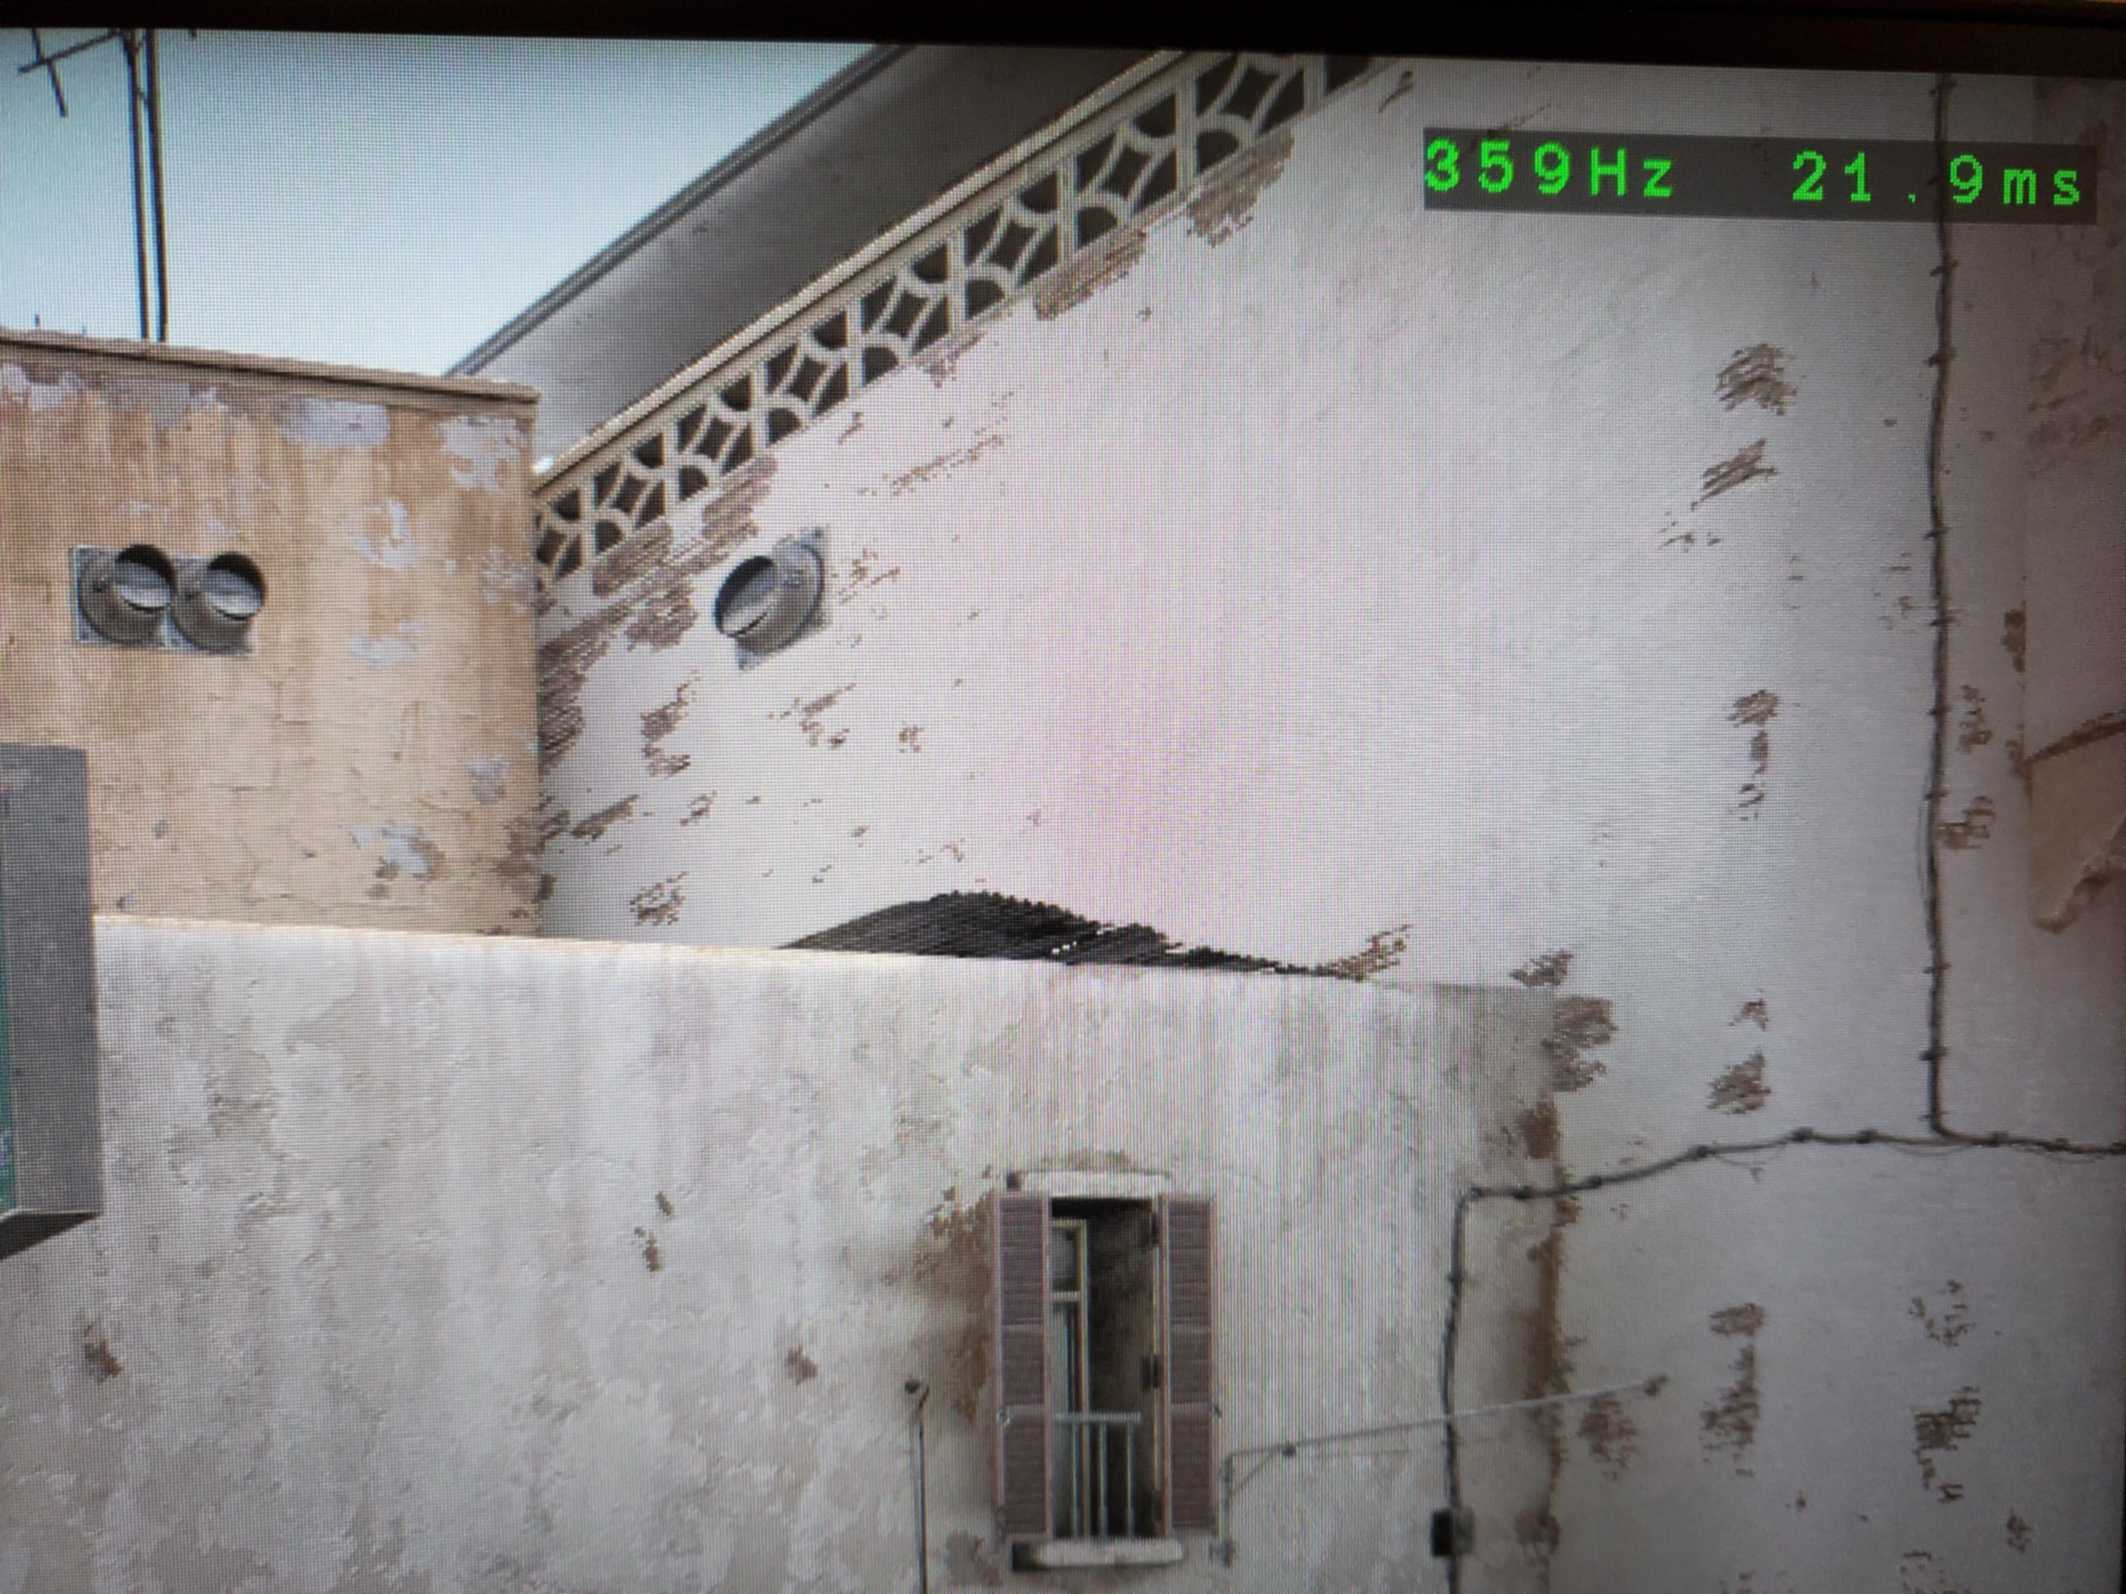
\includegraphics[width=0.8\textwidth]{StatoDellArte_files/nvreflex_example.jpg}
	\caption{Nvidia Reflex Latency Analyzer (da nvidia.com)}
	\label{fig:nvreflex_example}
\end{figure}

Nel momento in cui viene scritto questo paragrafo (aggiornato a Giugno 2021), Nvidia Reflex Latency Analyzer è sostanzialmente inesistente sul mercato poiché supporta pochi modelli di display e mouse, e sono molto costosi per quello che offrono. Il requisito di utilizzare Nvidia Geforce Experience per utilizzarlo, un'applicazione proprietaria che richiede un login e con una pessima reputazione, non ha sicuramente contribuito alla sua diffusione.

\section{DisplayCAL}
DisplayCAL\footnote{\url{https://displaycal.net/}} è un software libero di calibrazione e profilazione di display basato su ArgyllCMS\footnote{\url{https://www.argyllcms.com/}}.

Lo scopo principale di questa applicazione è quella di misurare l'accuratezza dei colori del display utilizzando un colorimetro o uno spettrofotometro tra quelli supportati da ArgyllCMS e generare un profilo di colore ICC che può essere utilizzato nel sistema operativo per fornire dei colori più accurati. Oltre alla calibrazione, può generare anche dei \textit{report} che mostrano il gamut del display, le curve di gamma, e molto altro, secondo molti standard.

La figura \ref{fig:displaycal_report_example} mostra un esempio di \textit{report} generato da DisplayCAL riguardante l'accuratezza dei colori. Il test consiste nel visualizzare una serie di colori e calcolare la differenza tra il colore visualizzato e quello inteso utilizzando qualche tecnica come Delta-E 1976, tenendo conto dello spazio colore in cui deve essere visualizzato.

\begin{figure}[h!]
	\centering
	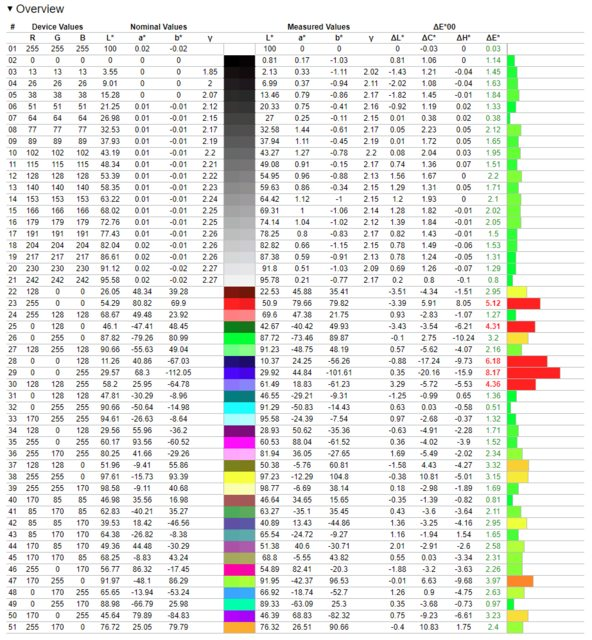
\includegraphics[width=0.8\textwidth]{StatoDellArte_files/displaycal_report_example.jpg}
	\caption{Esempio di \textit{report} sull'accuratezza dei colori di DisplayCAL}
	\label{fig:displaycal_report_example}
\end{figure}

Siccome questo software si concentra sulla qualità dell'immagine e soprattutto dei colori, il suo obiettivo è diverso rispetto a quello di Nvidia LDAT e di OpenLDAT, e non implementa alcun test riguardante le tempistiche del display e del sistema (Marzo 2021). I dispositivi supportati da DisplayCAL inoltre sono molto più sofisticati e piuttosto costosi, con i modelli più economici (dei colorimetri a tre canali) che partono da circa 100€.

\section{Dispositivo di RTINGS}
Il sito di recensioni RTINGS\footnote{\url{https://rtings.com/}} ha sviluppato un proprio dispositivo per eseguire diversi tipi di misurazioni sui display: tempi di latenza, tempi di risposta dei pixel, errore di transizione causato dall'\textit{overdrive}, e altro.

Purtroppo non sono note informazioni sul dispositivo stesso, ma è visibile in alcune fotografie presenti nelle recensioni, come quella in figura \ref{fig:rtings_device}. Sembra essere un sistema composto da un'MCU e da un sensore di luminosità. Non è noto come i dati raccolti dal sensore vengano analizzati (manualmente o da un programma apposito).

\begin{figure}[h!]
	\centering
	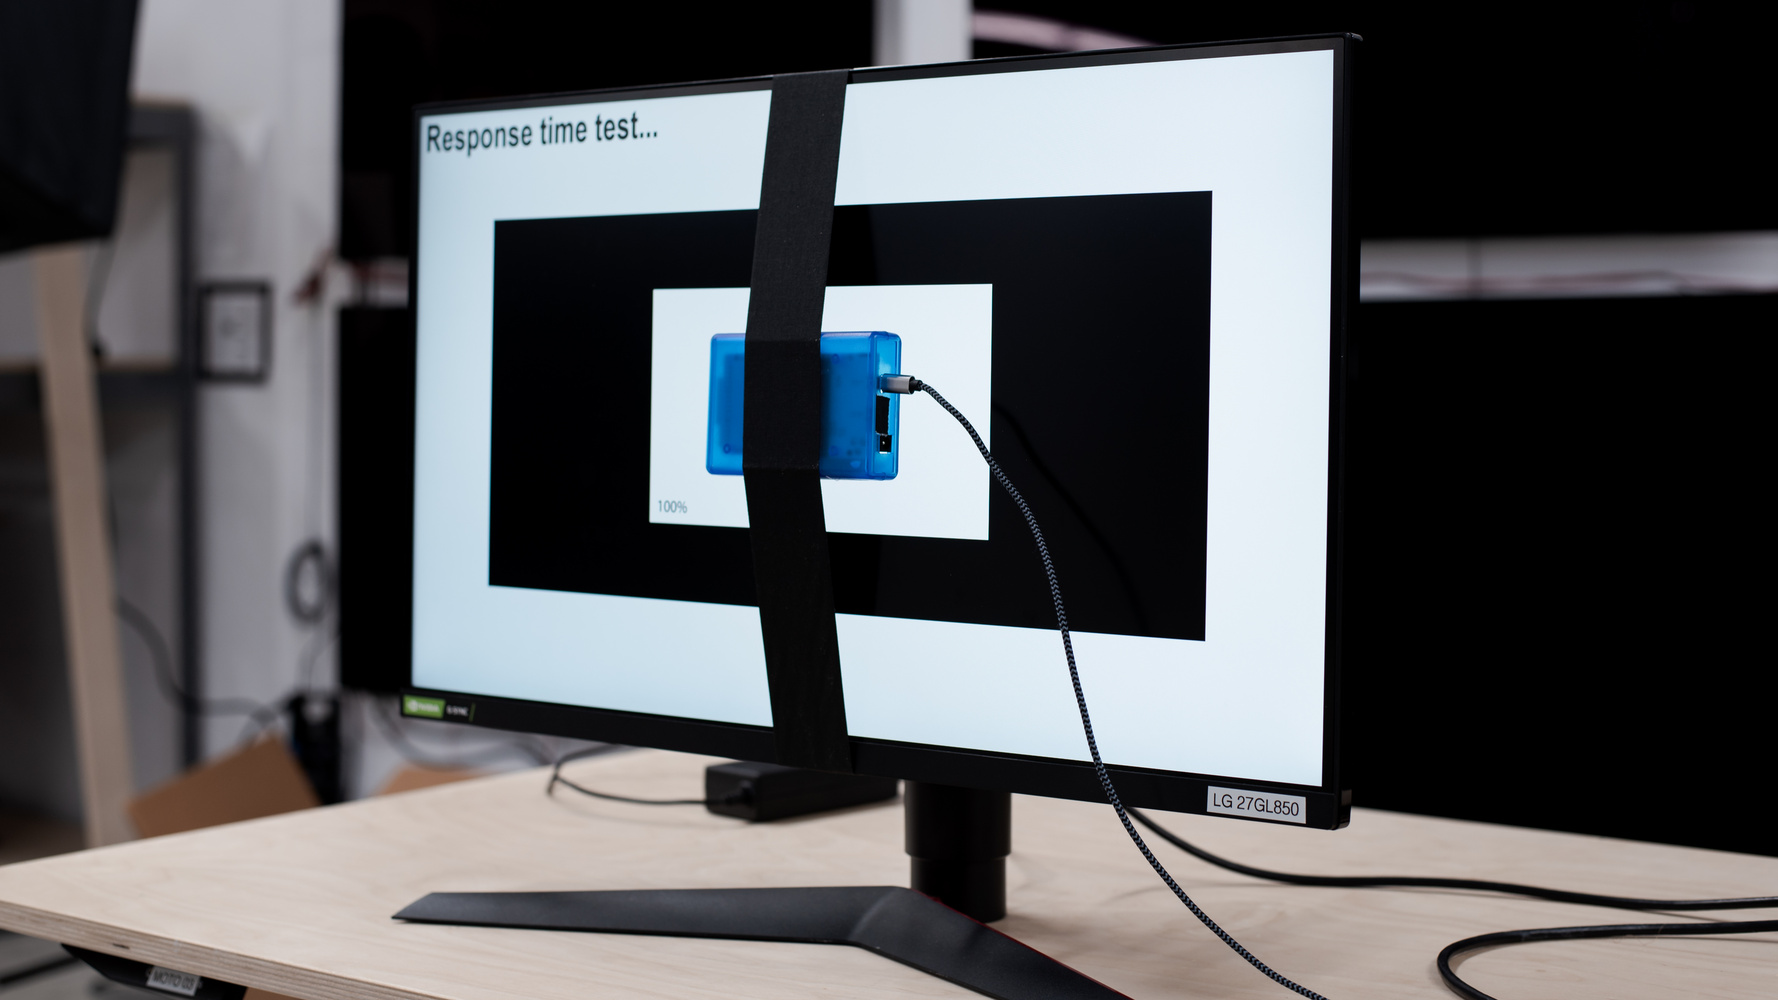
\includegraphics[width=0.8\textwidth]{StatoDellArte_files/rtings_device.jpg}
	\caption{Il dispositivo di RTINGS}
	\label{fig:rtings_device}
\end{figure}

Altri test nelle recensioni presenti sul sito vengono invece svolti utilizzando un colorimetro e DisplayCAL: luminosità, contrasto, curve di gamma, gamut, temperatura del bianco, e altro. Alcuni test infine sono eseguiti manualmente con una telecamera, come quello sugli angoli di visione.

Questo conclude il capitolo sullo stato dell'arte. I capitoli successivi si concentrano sul progetto OpenLDAT.

\newpage
\chapter{Il dispositivo OpenLDAT}
\label{chap:device}

In questo capitolo viene introdotto il dispositivo fisico OpenLDAT, descrivendone i requisiti, le caratteristiche, il funzionamento dell'hardware e del firmware e i passi necessari per realizzarlo a partire da un elenco di componenti.

Il dispositivo OpenLDAT ha sostanzialmente quattro compiti:
\begin{itemize}
	\item Campionare nel modo più regolare e veloce possibile un sensore di luminosità
	\item Generare dei click (automaticamente o manualmente a seconda del test), facendo finta di essere un mouse
	\item Far lampeggiare un LED sul dispositivo quando vengono generati click, in modo che le misurazioni sulla latenza siano verificabili usando una telecamera ad alta velocità
	\item Gestire la comunicazione con il PC, ricevendo comandi e inviando i dati del sensore e del mouse virtuale
\end{itemize}

Un obiettivo principale del progetto è anche far si che il dispositivo sia costruito usando componenti \textit{off-the-shelf}, con costi relativamente bassi (molto meno di un colorimetro), senza bisogno di apparecchiature speciali per la sua costruzione. In altre parole, deve essere costruibile nel tipico laboratorio di un maker.

\section{Hardware}
Alla base del dispositivo c'è uno Sparkfun Pro Micro 5V/16MHz: si tratta di una MCU Arduino-compatibile, open-hardware, basata sul microcontroller ATmega 32U4 e dotata di una connessione Micro-USB. La figura \ref{fig:sparkfun_promicro} mostra la board e le sue dimensioni molto ridotte.
\begin{figure}[h]
	\centering
	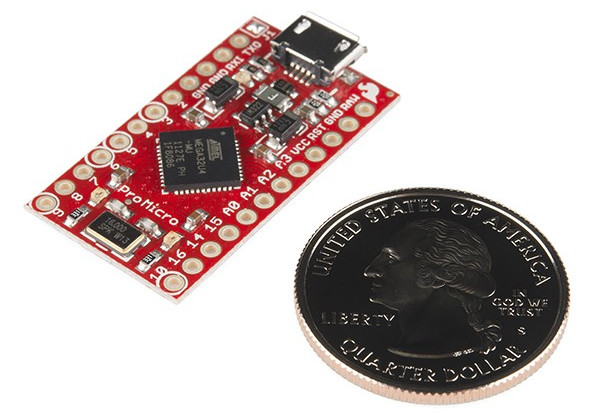
\includegraphics[width=0.7\textwidth]{Dispositivo_files/sparkfun_promicro.jpg}
	\caption{Sparkfun Pro Micro 5V/16MHz (da sparkfun.com)}
	\label{fig:sparkfun_promicro}
\end{figure}

La scelta di questa MCU non è casuale, per il progetto ci interessano le seguenti caratteristiche:
\begin{itemize}
	\item ADC per approssimazioni successive a 10 bit, con la possibilità di controllare via software il comportamento dell'ADC, variando così la velocità di campionamento e i tempi del circuito \textit{sample-and-hold}
	\item Timer configurabili per generare segnali di varia natura, anche di frequenza molto bassa
	\item Controller USB programmabile, così da poter simulare vari tipi di dispositivo (nel caso di OpenLDAT, una porta seriale e un mouse)
	\item Comunicazione via seriale asincrona rispetto all'esecuzione del firmware (entro certi limiti)
	\item Pin GPIO con supporto ad interrupt, \textit{pull-up} e logica \textit{tri-state}
	\item Alta disponibilità di cloni poco costosi
	\item Ampiamente documentato, sia dal produttore che dalla community, poiché è completamente compatibile con l'Arduino Leonardo
	\item Dimensioni ridotte, che consentono di creare un dispositivo di dimensioni ragionevoli e che riceve meno interferenze dall'esterno
\end{itemize}

Altre caratteristiche generali del microcontroller 32U4 sono:
\begin{itemize}
	\item Clock a 16MHz, con una velocità tipica di esecuzione delle istruzioni di 16MIPS
	\item 32kB di memoria flash, di cui 28KB disponibili al software e 4KB riservati al bootloader (che può essere rimosso)
	\item 2.5kB di RAM
	\item 1kB di EEPROM
\end{itemize}

Il secondo componente chiave è il sensore di luminosità Everlight ALS-PT19. Si tratta di un fototransistor dai tempi di risposta molto bassi, con una buona linearità e un costo molto contenuto. Poiché questo componente è SMD ed è estremamente piccolo, è stato scelto di usare il \textit{breakout} Adafruit ALS-PT19 mostrato in figura \ref{fig:adafruit_pt19}, che monta il sensore e una resistenza da 10k\si{\ohm} su un piccolo PCB, così da poterlo montare facilmente e avere un valore misurabile in tensione anziché in corrente. Variando il valore della resistenza tra il fototransistor e la massa, si regola la sensibilità del sensore (più è alta la resistenza e più è sensibile alla luce).
\begin{figure}[h]
	\centering
	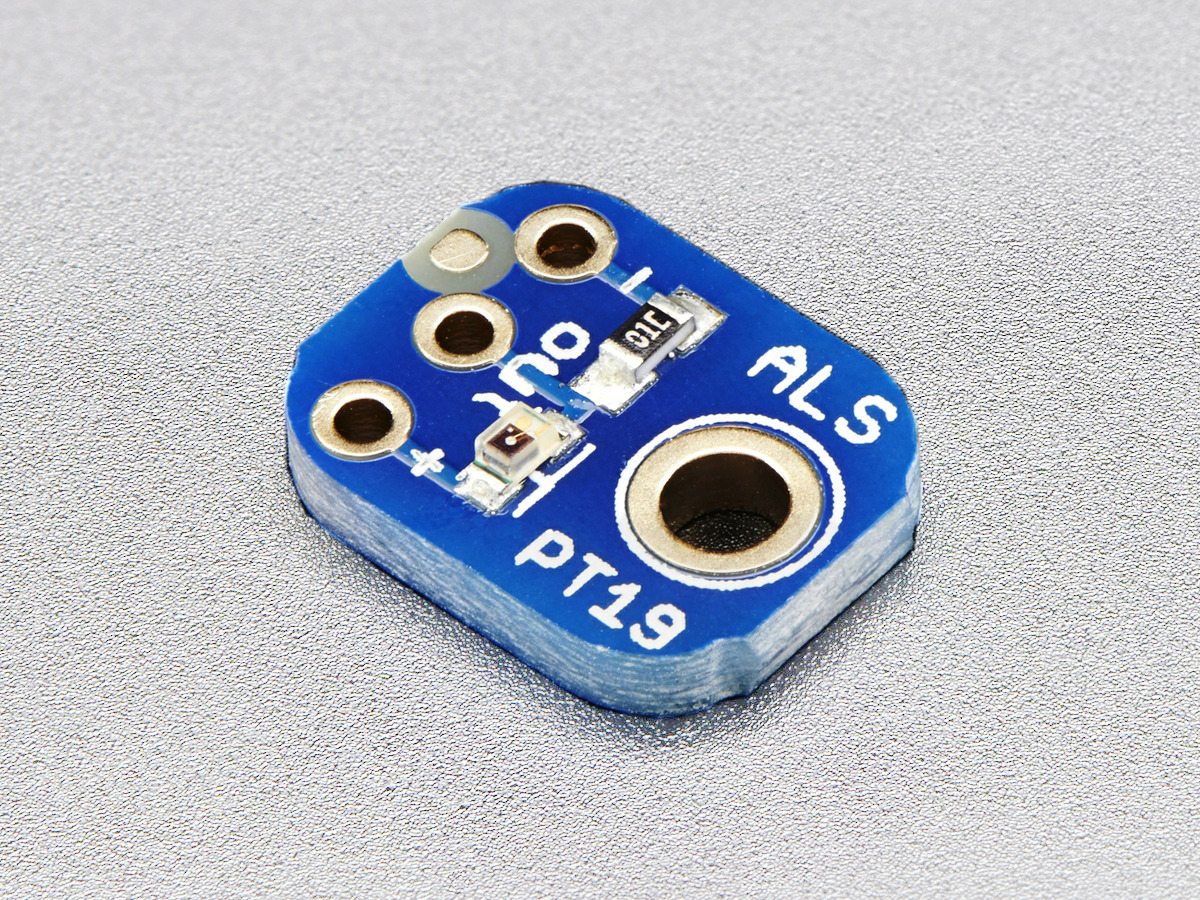
\includegraphics[width=0.7\textwidth]{Dispositivo_files/als-pt19.jpg}
	\caption{Adafruit ALS-PT19 (da adafruit.com)}
	\label{fig:adafruit_pt19}
\end{figure}

Il sensore ha un tempo di risposta di circa 0.1ms in salita e 0.2ms in discesa \cite{als_pt19_datasheet}, che è stato verificato collegandolo ad un oscilloscopio (mostrato in figura \ref{fig:sensor_scope_risefall}), quindi è sufficientemente veloce da poter misurare non solo la latenza totale del sistema, ma anche il comportamento della retroilluminazione e la risposta dei pixel, cosa che non era possibile usando un semplice fotoresistore.

\begin{figure}[h!]
	\centering
	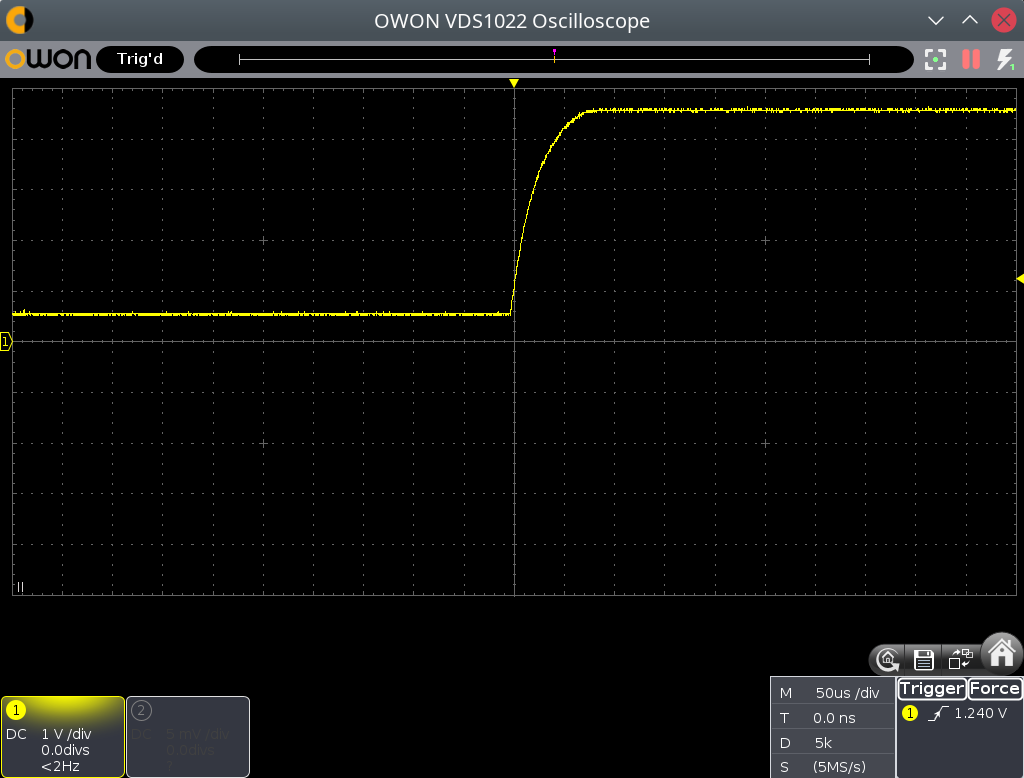
\includegraphics[width=0.75\textwidth]{Dispositivo_files/sensor_scope_rise.png}
	
	\vspace{0.2cm}
	
	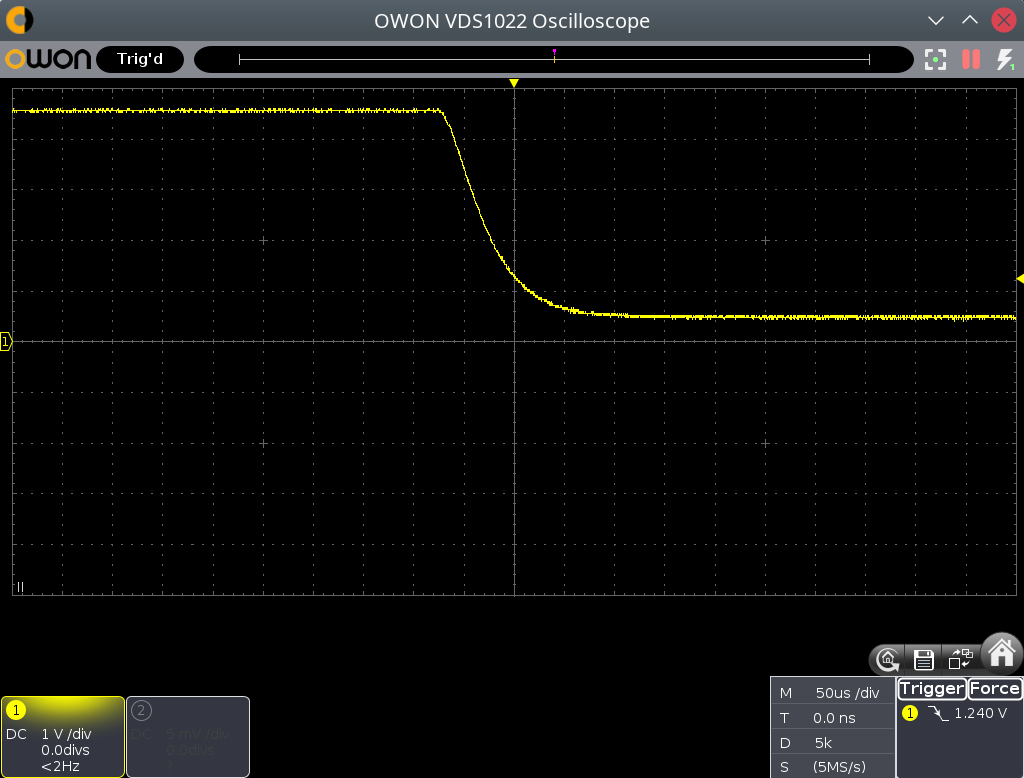
\includegraphics[width=0.75\textwidth]{Dispositivo_files/sensor_scope_fall.png}
	\caption{Salita e discesa del sensore ALS-PT19 catturata con un oscilloscopio}
	\label{fig:sensor_scope_risefall}
\end{figure}

La risposta spettrale del sensore non è particolarmente rilevante per questa applicazione, ma la documentazione mostra una risposta simile a quella dell'occhio umano, con un picco intorno alla lunghezza d'onda del verde \cite{als_pt19_datasheet}, tuttavia è anche sensibile alla luce ultravioletta.

La linearità è importante per questa applicazione. La documentazione del sensore mostra una buona linearità, ma avverte questa è affetta dalla temperatura ambiente e dal voltaggio che viene applicato \cite{als_pt19_datasheet}.\\
Per verificare che la linearità sia sufficiente per lo scopo, è stato realizzato un prototipo dotato del sensore stesso più un sensore AMS TCS34725. Pur non essendo neanche paragonabile ad un colorimetro professionale, questo sensore è calibrato di fabbrica e la misurazione della luminosità è molto lenta ma più accurata rispetto all'ALS-PT19 \cite{tcs34725_datasheet}.\\
Il grafico in figura \ref{fig:pt19_linearity} mostra sull'asse X la luminosità misurata dal TCS34725 e sull'asse Y quella misurata dall'ALS-PT19 (linea nera). Idealmente dovrebbe essere una linea retta priva di curve (linea rossa).

\begin{figure}[h!]
	\centering
	\begin{tikzpicture}
		\begin{axis}[name=ALS-PT19, xmin=0,xmax=300,ymin=0,ymax=5,width=.7\textwidth,xlabel=Luminosità,ylabel=Voltaggio (V)]
			\addplot[black] file{Dispositivo_files/pt19_linearity1.txt};
			\addplot[red] file{Dispositivo_files/pt19_linearity2.txt};
		\end{axis}
	\end{tikzpicture}
	\caption{Linearità del sensore ALS-PT19}
	\label{fig:pt19_linearity}
\end{figure}

Il grafico in figura \ref{fig:pt19_linearity3} mostra il rapporto tra la misurazione dell'ALS-PT19 e quella del TCS34725, e permette di vedere meglio che c'è una leggera sovrastima della misura sui valori di luminosità molto bassi, ma poi si stabilizza verso una misura sostanzialmente identica.
\begin{figure}[h!]
	\centering
	\begin{tikzpicture}
		\begin{axis}[name=Rapporto, xmin=0,xmax=300,ymin=0,ymax=2,width=.7\textwidth,xlabel=Luminosità]
			\addplot[black] file{Dispositivo_files/pt19_linearity3.txt};
		\end{axis}
	\end{tikzpicture}
	\caption{Rapporto tra ALS-PT19 e TCS34725}
	\label{fig:pt19_linearity3}
\end{figure}

Va inoltre verificato il comportamento man mano che ci si avvicina alla soglia di saturazione. Nella documentazione viene dichiarato che il sensore si comporta linearmente fino alla soglia di saturazione dichiarata di circa 4.75V\cite{als_pt19_datasheet}, ma nella realtà la saturazione comincia a manifestarsi intorno ai 4V, per cui il software deve tenerne conto. Il grafico in figura \ref{fig:pt19_linearity4} mostra la perdita di linearità mentre si avvicina alla soglia di saturazione (Nota: è stata usata una resistenza di alto valore per aumentare il guadagno del sensore).

\begin{figure}[h!]
	\centering
	\begin{tikzpicture}
		\begin{axis}[name=ALS-PT19, xmin=0,xmax=300,ymin=0,ymax=5,width=.7\textwidth,xlabel=Luminosità,ylabel=Voltaggio (V)]
			\addplot[black] file{Dispositivo_files/pt19_linearity4.txt};
		\end{axis}
	\end{tikzpicture}
	\caption{Saturazione dell'ALS-PT19}
	\label{fig:pt19_linearity4}
\end{figure}

Questi test sono stati eseguiti leggendo entrambi i sensori contemporaneamente, utilizzando un display in una stanza buia come sorgente luminosa. Il sensore TCS34725 ha il proprio ADC, mentre l'ALS-PT19, essendo un sensore completamente analogico, utilizza uno degli ingressi dell'ADC del microcontroller 32U4. La temperatura ambiente durante i test era di 21°C e il voltaggio applicato ai sensori era 5V. Eventuali errori causati dagli ADC stessi o dalle differenze tra i due ADC non sono misurabili in questo test. Sono stati testati tre ALS-PT19 provenienti da venditori diversi ottenendo risultati virtualmente identici.

\subsection{Schema elettrico}
L'ultimo componente essenziale per il dispositivo OpenLDAT è un circuito (stampato o fatto a mano) che collega tutti i componenti. Questo circuito deve:
\begin{itemize}
	\item Collegare il microcontroller al sensore
	\item Permettere al microcontroller di variare il guadagno del sensore selezionando delle resistenze
	\item Far lampeggiare un LED in corrispondenza ai click (automatici o manuali)
	\item Permettere all'utente di connettere un mouse o un pulsante esterno per generare click manualmente
\end{itemize}

La figura \ref{fig:circuit} mostra lo schema elettrico del circuito che è stato realizzato.
\begin{figure}[h]
	\centering
	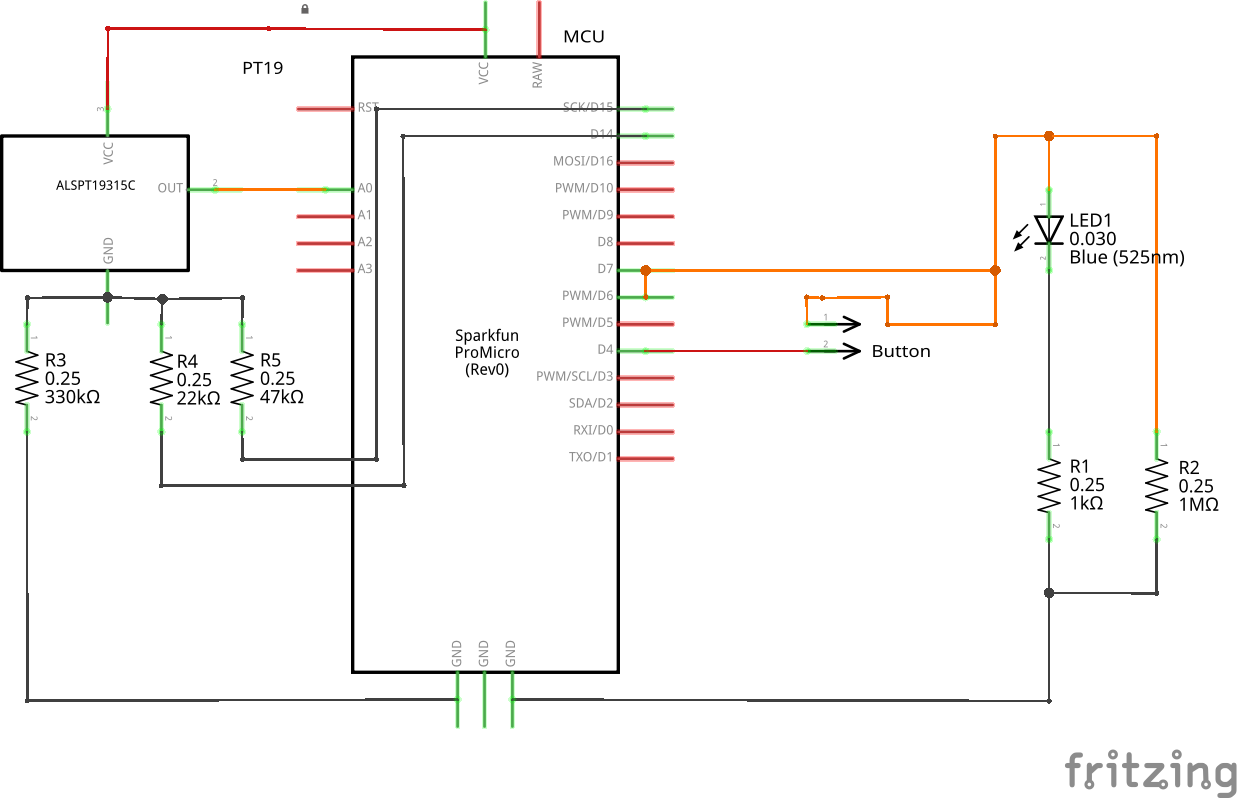
\includegraphics[width=\textwidth]{Dispositivo_files/openldat_circuit.png}
	\caption{Schema elettrico del dispositivo OpenLDAT}
	\label{fig:circuit}
\end{figure}

La regolazione del gain del sensore avviene mediante le resistenze R3 (330k\si{\ohm}), R4 (22k\si{\ohm}) e R5 (47k\si{\ohm}), posizionate in parallelo in serie alla resistenza da 10k\si{\ohm} già presente sul PCB dell'ALS-PT19. R3 è permanentemente connessa a massa, mentre R4 e R5 possono essere attivate e disattivate controllando lo stato dei pin D14 e D15 rispettivamente. Un pin GPIO in stato \texttt{LOW} equivale ad un collegamento a massa di resistenza trascurabile, mentre un pin in stato \texttt{Z} equivale ad un pin disconnesso (la documentazione del microcontroller indica un'impedenza di 100M\si{\ohm} in questo stato). Svolgendo i calcoli si possono stimare i quattro possibli valori di resistenza davanti al sensore, mostrati in tabella \ref{tab:pt19_gains}. Questi valori sono ovviamente delle stime e non tengono conto delle tolleranze di produzione delle resistenze e del microcontroller.
\begin{table}
	\centering
	\begin{tabular}{|c|c|c|} 
		\hline
		\textbf{Configurazione (D14,D15)} & \textbf{Resistenza (k\si{\ohm})} & \textbf{Gain relativo}  \\ 
		\hline
		L,L & 24.334   & 1.000         \\ 
		\hline
		Z,L & 30.620   & 1.258         \\ 
		\hline
		L,Z & 51.123   & 2.101         \\ 
		\hline
		Z,Z & 337.847    & 13.883          \\
		\hline
	\end{tabular}
	\caption{\label{tab:pt19_gains}Livelli di gain implementati}
\end{table}

Conoscendo il tipo di luce che genera la retroilluminazione del display (si assume LED con temperatura del bianco neutra), la resistenza usata per il gain e la precisione dell'ADC, è possibile stimare molto grossolanamente quali sono i livelli di luminosità massima raccomandabili per ogni livello di gain, mostrati in tabella \ref{tab:pt19_nits}. Generalmente i due livelli di gain più elevati sono sufficienti per la maggior parte dei display, mentre quelli più bassi sono utili solo su display HDR.
\begin{table}
	\centering
	\begin{tabular}{|c|c|} 
		\hline
		\textbf{Gain relativo} & \textbf{Luminosità consigliabile (nits)}  \\ 
		\hline
		1.000 & 300-700         \\ 
		\hline
		1.258 & 250-600         \\ 
		\hline
		2.101 & 60-300         \\ 
		\hline
		13.883 & 0-80          \\
		\hline
	\end{tabular}
	\caption{\label{tab:pt19_nits}Range di luminosità del display consigliabile per ogni livello di gain}
\end{table}

La generazione dei click interna e esterna al dispositivo e il lampeggio del LED sono gestiti sulla parte destra dello schema in figura \ref{fig:circuit}. I click vengono captati tramite interrupt sul pin D7. Sfruttando la logica tri-state dei pin GPIO è possibile utilizzare lo stesso circuito per gestire sia i click automatici che quelli manuali:
\begin{itemize}
	\item Quando il dispositivo genera autonomamente i click, un timer interno al microcontroller manda brevi pulsazioni a una frequenza di circa 1Hz dal pin D6, e quindi varia tra gli stati \texttt{HIGH} e \texttt{LOW}, mentre il pin D4 è posizionato in stato \texttt{Z}, come se fosse disconnesso. Quando il segnale dal pin D6 passa ad \texttt{HIGH}, D7 riceve l'interrupt, e contemporaneamente si accende il LED. I pin per il pulsante sono inattivi in questa modalità, e cortocircuitarli non ha alcun effetto sul dispositivo
	\item Quando il dispositivo riceve i click dall'esterno, il pin D4 è in stato \texttt{HIGH} per fornire alimentazione al pulsante esterno, mentre il pin D6 è in stato Z, come se fosse disconnesso. Quando il pulsante esterno viene premuto, i due contatti per il pulsante vengono cortocircuitati, D7 riceve l'interrupt, e contemporaneamente si accende il LED
\end{itemize}

La resistenza R1 serve per limitare la luminosità del LED, mentre la resistenza R2 fa da \textit{pull-down} per evitare che il pin D7 vada in stato floating quando si ricevono i click dall'esterno e il pulsante esterno non è premuto.

Poiché il lampeggio del LED è gestito in modo totalmente analogico, non c'è ritardo introdotto dal firmware.

\subsection{PCB}
Il circuito può essere stampato su un PCB a singolo strato delle dimensioni di 23x41mm e uno spessore di 1.6mm, su cui poi si saldano i componenti. Il PCB è pensato per essere semplice da realizzare anche in casa se si hanno gli strumenti per farlo, non è necessario utilizzare servizi di produzione professionali.

La figura \ref{fig:pcb} mostra due viste del PCB da sopra e da sotto: sul lato superiore sono presenti la board con il microcontroller, i pin per il mouse esterno e il LED, mentre sul lato inferiore sono presenti il \textit{breakout} con il sensore ALS-PT19 e le varie resistenze per controllarne il gain. Tutte le piste che collegano i componenti sono sul lato inferiore.
\begin{figure}[h]
	\centering
	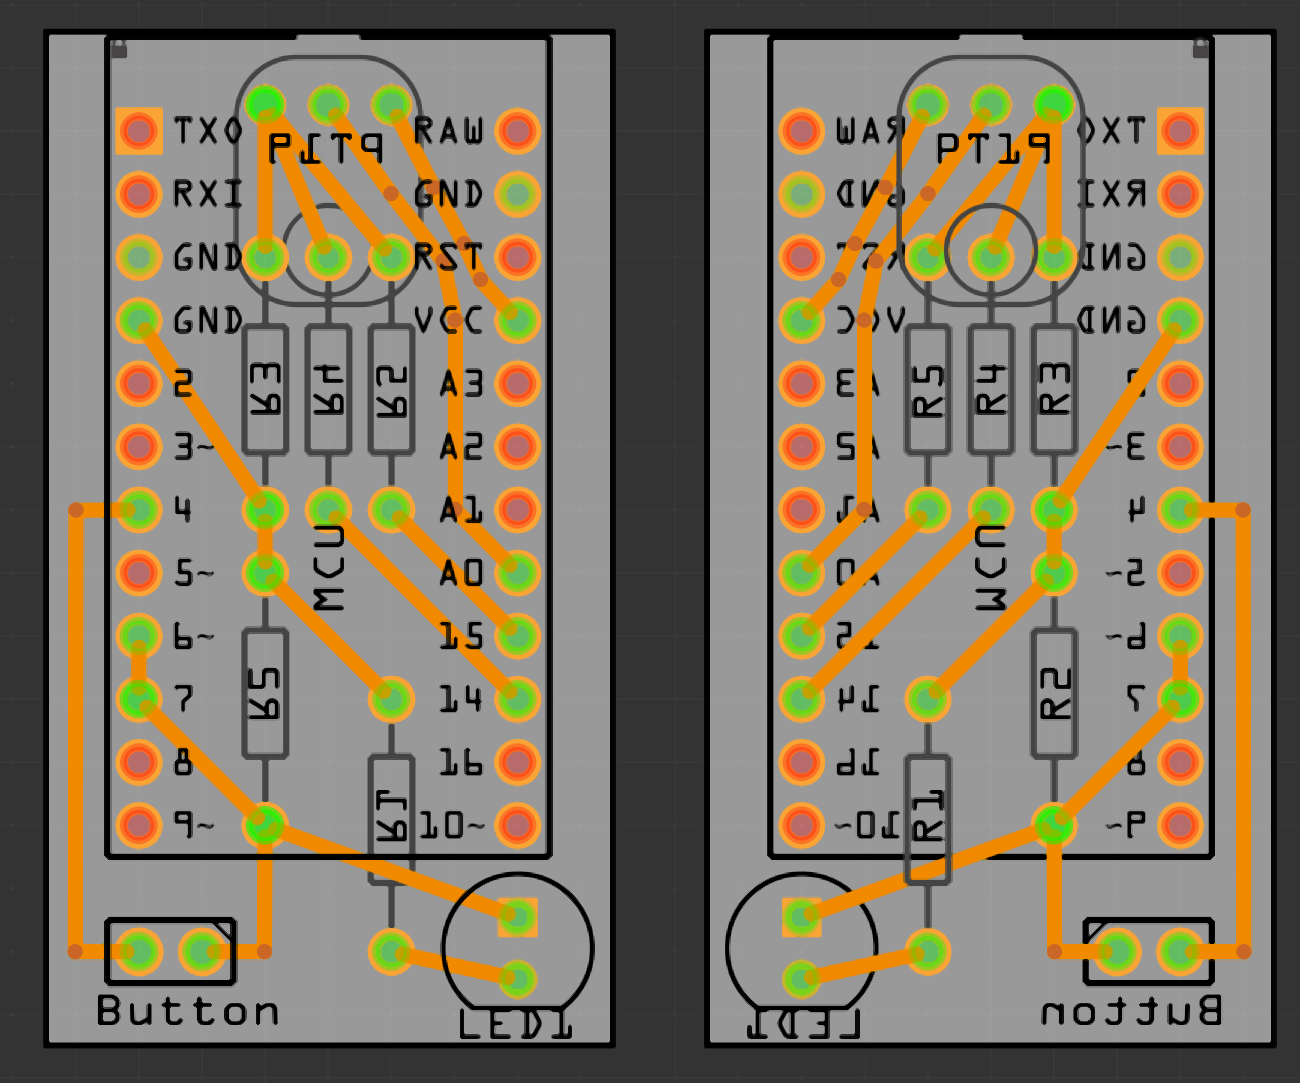
\includegraphics[width=\textwidth]{Dispositivo_files/openldat_pcb.png}
	\caption{Il PCB del dispositivo OpenLDAT visto da sopra e da sotto}
	\label{fig:pcb}
\end{figure}

\subsection{Case}
È stato realizzato un case per il dispositivo stampabile con una stampante 3D, progettato per essere facile da stampare e montare, che minimizzi le infiltrazioni di luce indesiderate, e che permetta di appoggiare il dispositivo sullo schermo da testare senza rischiare di graffiarne il vetro.

Il case è composto da tre parti (di cui una opzionale):
\begin{itemize}
	\item La base (figura \ref{fig:case_base}): è la parte principale, dalla forma circolare con un diametro di 59mm e un'altezza di 21mm, con quattro supporti in cui incastrare il PCB, due supporti laterali in cui incastrare il coperchio, un foro di 14x14mm sulla parte inferiore dove può passare la luce verso il sensore, e uno sul lato per la porta USB. Attorno al foro per il sensore è presente un piccolo incavo in cui è possibile, opzionalmente, incollare un vetrino da microscopio 22x22mm per proteggere il sensore. Sempre opzionalmente, è possibile posizionare dei feltrini sottili o del velluto sulla parte che si appoggia sullo schermo, per un'ulteriore protezione contro graffi accidentali
	\item Il coperchio (figura \ref{fig:case_top}): si incastra nei due supporti laterali e permette di bloccare la luce dall'esterno. Due fori consentono il collegamento del pulsante esterno e rendono visibile il LED sul dispositivo, due barrette tengono fermo il PCB, qualora dovesse uscire dagli incastri della base
	\item Diffusore per il LED (figura \ref{fig:case_ledcover}): un piccolo pezzo di plastica trasparente, del tutto opzionale, che può essere incastrato nel foro per il LED presente sul coperchio, così da rendere più esteticamente piacevole la luce del LED del dispositivo. Rende inoltre visibile la luce dei LED sulla MCU, che si illuminano durante la comunicazione con il PC
\end{itemize}

Se stampato correttamente, la distribuzione del peso del case stesso gli permette di stare fermo quando è appoggiato al display.

\begin{figure}[H]
	\centering
	\adjincludegraphics[trim={{.10\width} 0 0 0},clip,width=\textwidth]{Dispositivo_files/openldat_case_base1.jpg}
	\caption{Base del case}
	\label{fig:case_base}
\end{figure}
\begin{figure}[H]
	\centering
	\adjincludegraphics[trim={{.10\width} 0 0 0},clip,width=\textwidth]{Dispositivo_files/openldat_case_top1.jpg}
	
	\vspace{0.5cm}
	
	\adjincludegraphics[trim={{.10\width} 0 0 0},clip,width=\textwidth]{Dispositivo_files/openldat_case_top2.jpg}
	\caption{Coperchio del case}
	\label{fig:case_top}
\end{figure}
\begin{figure}[H]
	\centering
	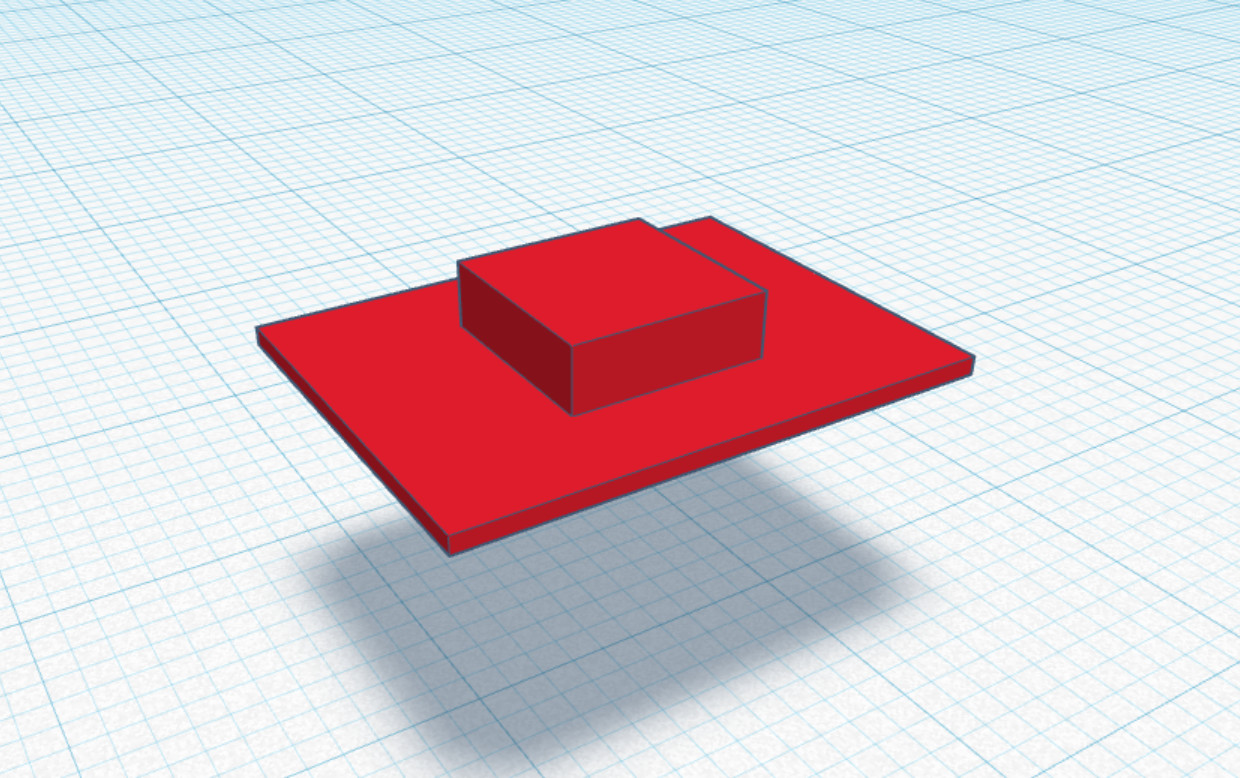
\includegraphics[width=\textwidth]{Dispositivo_files/openldat_case_ledcover.jpg}
	\caption{Diffusore trasparente per il LED (opzionale)}
	\label{fig:case_ledcover}
\end{figure}

\subsection{Bill Of Materials}
La tabella \ref{tab:bom} mostra tutto il materiale necessario per costruire il dispositivo OpenLDAT. I prezzi sono aggiornati a Aprile 2021 e variano molto a seconda delle quantità ordinate (la tabella fa riferimento a un ordine per i componenti per assemblare 9-10 dispositivi). Non tutti i componenti sono essenziali.

\begin{table}[h!]
	\centering
	\resizebox{\columnwidth}{!}{\begin{tabular}{|l|l|l|l|} 
		\hline
		\textbf{Essenziale} & \textbf{Nome} & \textbf{Fornitore} & \textbf{Prezzo (€)}  \\ 
		\hline
		Si & Sparkfun Pro Micro 5V/16MHz (clone) con header & Aliexpress (\textit{keyword}: 32u4) & 4.98         \\ 
		\hline
		Si & Adafruit ALS-PT19 con header & Aliexpress (\textit{keyword}: als pt19) & 2.28         \\
		\hline
		Si & PCB OpenLDAT & Aisler & 2.45        \\
		\hline
		Si & Resistenze ¼W: 1M\si{\ohm}, 1k\si{\ohm}, 330k\si{\ohm}, 22k\si{\ohm}, 47k\si{\ohm} & Qualsiasi & 0.10        \\
		\hline
		Si & 2 pin header maschio & Inclusi col sensore & 0.00\\
		\hline
		Si & LED 5mm (qualsiasi colore) & Qualsiasi & 0.02 \\
		\hline
		No & 50g PLA Nero & Amazon (marca GIANTARM) & 0.90        \\
		\hline
		No & 2g PLA Trasparente & Amazon (marca GIANTARM) & 0.04        \\
		\hline
		No & Vetrino coprioggetto per microscopio 22x22mm & Amazon & 0.05        \\
		\hline
	\end{tabular}}
	\caption{\label{tab:bom}Materiali per la realizzazione il dispositivo OpenLDAT}
\end{table}

\subsection{Costruzione del mouse modificato}
Per misurare la latenza di una macchina separata è necessario modificare un mouse (o volendo un controller) in modo che quando viene premuto il tasto per fare fuoco vengano cortocircuitati i due pin per il pulsante esterno sul dispositivo OpenLDAT. Eseguire questa modifica richiede un minimo di competenze elettroniche poiché ogni modello di mouse è diverso: nei casi più semplici è possibile collegare i contatti del pulsante ai pin del dispositivo, ma più in generale è consigliabile l'uso di un \textit{analog switch} come l'integrato Vishay DG213DJ\cite{vishay_dg213_datasheet}, il quale può essere alimentato direttamente dal mouse, può gestire sia segnali normalmente alti che normalmente bassi, e può cortocircuitare i pin del pulsante esterno in risposta ai click in totale sicurezza. È sconsigliabile l'uso di optoisolatori, filtri RC, o qualsiasi altro costrutto che potrebbe ritardare il segnale di più di qualche microsecondo.\\
Sul dispositivo OpenLDAT, il pin di sinistra porta un segnale \texttt{HIGH} (5V), mentre il pin di destra è in alta impedenza in attesa di ricevere il segnale. La soglia di attivazione del pin di destra è circa 3V\cite{atmega32u4_datasheet}. La quantità di corrente che può passare è limitata a pochi mA dal LED e dalle resistenze presenti tra il pin di destra e la massa.\\
Il circuito in figura \ref{fig:modmouse_example} mostra un esempio di circuito per un mouse modificato, ma potrebbe variare molto tra mouse diversi: potrebbe essere necessario cambiare o rimuovere la resistenza in input o creare un \textit{pull-up}/\textit{pull-down}, o costruire un circuito totalmente diverso.

\begin{figure}[h!]
	\centering
	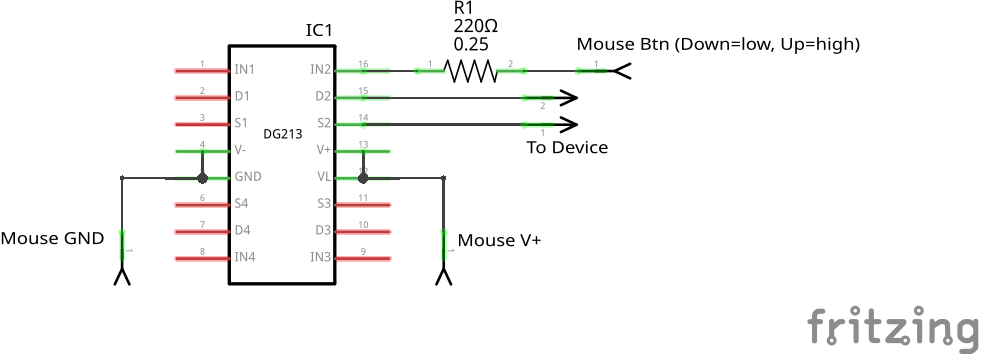
\includegraphics[width=\textwidth]{Dispositivo_files/modmouse_example.png}
	\caption{Esempio di circuito per mouse modificato}
	\label{fig:modmouse_example}
\end{figure}

Una volta assemblato, il circuito può essere nascosto all'interno del mouse, lasciando uscire solo i cavi da connettere sul dispositivo OpenLDAT.

Attenzione: un circuito errato potrebbe danneggiare permanentemente il dispositivo OpenLDAT e/o il mouse.

\section{Firmware}
Il firmware installato sul microcontroller ATmega 32U4 è stato sviluppato in C++ usando Arduino IDE e ha i seguenti compiti:
\begin{itemize}
	\item Permettere all'applicazione di identificare i dispositivi OpenLDAT connessi e le loro \textit{capability}
	\item Ricevere comandi dall'applicazione e inviare l'output via seriale
	\item Configurare l'hardware per le varie modalità di funzionamento (ADC, gain del sensore, generazione automatica o manuale dei click)
	\item Campionare il sensore (e se richiesto il bottone esterno) nel modo più veloce e regolare possibile
	\item Consentire la misurazione di metriche di velocità del dispositivo senza influire sul suo funzionamento
	\item Essere facilmente estensibile, per permettere l'aggiunta di altri sensori in versioni future del dispositivo
\end{itemize}

Il progetto si trova nella cartella \texttt{Device/Firmware/OpenLDAT} del repository ed è composto da 4 file:
\begin{itemize}
	\item \texttt{OpenLDAT.ino}: è il file principale del firmware, importa gli altri file del progetto, implementa la ricezione dei comandi dall'applicazione e il listing delle \textit{capability}
	\item \texttt{BuildConfig.h}: permette di attivare/disattivare alcune funzioni del firmware e dichiara alcune variabili globali, come il numero di versione
	\item \texttt{OscilloscopeDebug.h}: implementa delle macro che sono utilizzate all'interno del codice quando viene compilato con il debug con oscilloscopio attivo. Queste macro consentono di collegare un oscilloscopio al pin 10 della board del microcontroller e ottenere informazioni sui tempi di campionamento senza rallentare il funzionamento del dispositivo. Il funzionamento verrà discusso meglio in seguito
	\item \texttt{LightSensor.h}: contiene tutto il codice di configurazione e campionamento del sensore di luminosità, del pulsante esterno e dei click automatici
\end{itemize}

\subsection{Formato dei comandi}
I comandi che l'applicazione può mandare al dispositivo sono composti da 2 o più byte:
\begin{itemize}
	\item Il primo byte identifica il comando. Nella versione attuale sono implementati tre comandi: \begin{itemize}
		\item \texttt{IDLE} (0x49): interrompe qualsiasi attività in corso e si prepara a ricevere un nuovo comando
		\item \texttt{ID} (0x44): invia informazioni sul dispositivo e le sue \textit{capability} all'applicazione, poi si prepara a ricevere un nuovo comando
		\item \texttt{LIGHTSENSOR} (0x4C): configura il dispositivo e avvia il campionamento. L'esecuzione di questo comando continua fino a quando non viene ricevuto un nuovo comando
	\end{itemize}
	Eventuali comandi non validi vengono ignorati
	\item Il secondo byte contiene dei flag il cui significato dipende dal comando selezionato, verranno discussi in seguito
	\item Opzionalmente, possono seguire ulteriori byte di informazioni specifiche del comando selezionato. Nessuno dei comandi attualmente implementati fa uso di questa funzione
\end{itemize}

\subsection{Identificazione del dispositivo}
L'identificazione del dispositivo da parte dell'applicazione avviene in due fasi:
\begin{itemize}
	\item I dispositivi OpenLDAT vengono trovati in base all'ID hardware personalizzato. Il dispositivo si dichiara con il nome ``OpenLDAT Model 1'' e ID hardware (VID:PID) 4370:0001, il che lo rende facilmente distinguibile da altri dispositivi basati sulla stessa board che potrebbero essere connessi al PC. La figura \ref{fig:lsusb} mostra un output del comando \texttt{lsusb} di GNU/Linux mentre il dispositivo è connesso. Non è necessario installare nessun driver per comunicare col dispositivo
	\item Una volta stabilita la connessione, l'applicazione utilizza il comando \texttt{ID} per chiedere al dispositivo le sue \textit{capability}, in base alle quale decide se il dispositivo è supportato. Il formato di questo elenco verrà discusso nel paragrafo successivo.
\end{itemize}

\begin{figure}[h]
	\centering
	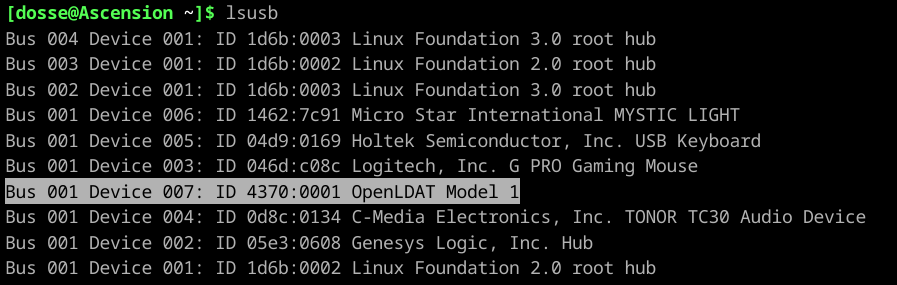
\includegraphics[width=0.8\textwidth]{Dispositivo_files/lsusb.png}
	\caption{Elenco di dispositivi USB, tra cui un OpenLDAT}
	\label{fig:lsusb}
\end{figure}

L'elenco delle \textit{capability} è inviato come testo ASCII. Il seguente listato mostra un possibile output del comando \texttt{ID}.
\lstinputlisting{Dispositivo_files/id_example.txt}
L'elenco è un insieme di stringhe ASCII, separate da un carattere \textit{newline} (\texttt{\textbackslash n}) e terminate da una riga vuota (doppio \textit{newline}). La prima riga contiene il nome completo del dispositivo, mentre le righe successive sono un elenco di \textit{capability} in formato \texttt{Nome: Valore}.

Le \textit{capability} attualmente implementate sono le seguenti:
\begin{itemize}
	\item \texttt{FW}: stringa contenente la versione del firmware del dispositivo, obbligatoria
	\item \texttt{LightSensor}: booleano che indica se è presente il sensore di luminosità. Se è presente, devono essere presenti anche le proprietà \texttt{LBuffer} e \texttt{SBuffer}, due interi il cui significato verrà spiegato nella sezione sul campionamento
	\item \texttt{OscilloscopeDebug}: booleano che indica se è possibile collegare un oscilloscopio al pin 10 per ottenere metriche sulle tempistiche del dispositivo
	\item \texttt{SerialDebug}: booleano che indica se il firmware è pensato per comunicare manualmente tramite il \textit{serial plotter} di Arduino IDE oppure se è pensato per comunicare con l'applicazione. Rallenta notevolmente l'esecuzione del firmware
	\item \texttt{Prototype}: booleano che indica se il dispositivo è un prototipo o una versione finale. Per i prototipi sono disponibili delle funzionalità aggiuntive nell'applicazione
	\item \texttt{MinAppVer}: intero che indica la versione del driver minima richiesta da questo dispositivo, obbligatorio
	\item \texttt{SerialNo}: stringa contenente il numero di serie del dispositivo (letto dalla EEPROM), oppure \texttt{DIY} se è stato assemblato a mano
\end{itemize}

\subsection{Configurazione e campionamento del sensore}
All'accensione del dispositivo, il codice di inizializzazione avvia un'interfaccia USB HID mouse per simulare i click e un'interfaccia seriale, così che possa comunicare con l'applicazione. Una caratteristica del microcontroller 32U4 è che utilizza l'USB CDC serial, per cui la comunicazione seriale avviene alla velocità del bus USB, e non ai baudrate della RS-232 come avviene nell'Arduino Uno. Questo consente una comunicazione molto più rapida ed evita di introdurre ritardi nel codice.

Il comando \texttt{LIGHTSENSOR} viene inviato dall'applicazione al dispositivo quando vuole utilizzare il sensore. Questo comando ha 7 possibili flag, che sono usati per configurare il dispositivo in vari modi. Considerando il byte di flag che segue il comando, partendo dal bit 0 (LSB) arrivando al bit 7 (MSB):
\begin{itemize}
	\item \textbf{Bit 0 (LSB)}: \texttt{AUTOFIRE}. Quando è impostato a 1, il dispositivo genera i click automaticamente, altrimenti li riceve dal pulsante esterno. Il valore di questo flag è ignorato se il flag \texttt{MONITOR} è impostato a 1
	\item \textbf{Bit 1}: \texttt{NOBUFFER}. Quando è impostato a 1, invia ogni sample immediatamente (più lento) anziché aspettare di aver riempito un buffer da mandare in blocco (più veloce)
	\item \textbf{Bit 2}: \texttt{HIGHSENS1}. Controlla la resistenza da 22k\si{\ohm} collegata al pin D14. Se è impostato a 1, la resistenza è attiva, aumentando il gain. Assieme al flag \texttt{HIGHSENS2} permette di selezionare 4 livelli di gain del sensore
	\item \textbf{Bit 3}: \texttt{MONITOR}. Quando è impostato a 1, viene letto il sensore ignorando i click (interni o esterni). Permette una lettura più veloce del sensore
	\item \textbf{Bit 4}: \texttt{NOCLICK}. Quando è impostato a 1, i click non vengono inviati tramite l'interfaccia USB HID mouse. I click sono comunque visibili sul LED e sull'interfaccia seriale. Il valore di questo flag è ignorato se il flag \texttt{MONITOR} è impostato a 1
	\item \textbf{Bit 5}: \texttt{FASTADC}. Quando è impostato a 1, configura l'ADC del microcontroller 32U4 per campionare molto più velocemente di quanto farebbe normalmente, consentendo velocità di campionamento fino a circa 30kHz
	\item \textbf{Bit 6}: \texttt{HIGHSENS2}. Controlla la resistenza da 47k\si{\ohm} collegata al pin D15. Se è impostato a 1, la resistenza è attiva, aumentando il gain. Assieme al flag \texttt{HIGHSENS1} permette di selezionare 4 livelli di gain del sensore
	\item \textbf{Bit 7 (MSB)}: Riservato per uso futuro (sempre 0 nella versione attuale)
\end{itemize}

Combinando i flag \texttt{NOBUFFER}, \texttt{FASTADC} e \texttt{MONITOR} in diversi modi, si possono ottenere 8 possibili velocità di campionamento, mostrate in tabella \ref{tab:openldat_samplerates}.
\begin{table}[h!]
	\centering
	\begin{tabular}{|c|c|c|c|c|} 
		\hline
		\texttt{NOBUFFER} & \texttt{FASTADC} & \texttt{MONITOR} & \textbf{Sample rate effettivo} & \textbf{Campionamento}   \\ 
		\hline
		1 & 0 & 0 & 7796.0Hz & 100\%         \\
		\hline
		1 & 0 & 1 & 7798.0Hz & 100\%         \\
		\hline
		1 & 1 & 0 & 20710.0Hz & 100\%         \\
		\hline
		1 & 1 & 1 & 21000.0Hz & 100\%         \\ 
		\hline
		0 & 0 & 0 & 8738.1Hz (416.1buf/s) & 97.92\%         \\
		\hline
		0 & 0 & 1 & 8758.4Hz (274.4buf/s) & 98.52\%         \\
		\hline
		0 & 1 & 0 & 28896.0Hz (1376.0buf/s) & 93.12\%         \\
		\hline
		0 & 1 & 1 & 29524.4Hz (924.2buf/s) & 95.01\%         \\
		\hline
	\end{tabular}
	\caption{\label{tab:openldat_samplerates}Velocità di campionamento}
\end{table}

Il flag \texttt{NOBUFFER} permette di attivare o disattivare il buffering sul dispositivo dei dati da mandare al PC. L'interfaccia seriale del microcontroller possiede due buffer di 64 byte (uno in ingresso e uno in uscita), e finché il buffer di scrittura non è pieno, le operazioni di scrittura su seriale non sono bloccanti, ma richiedono comunque del tempo per la copia dei dati sul buffer della seriale. Il firmware del dispositivo offre quindi una modalità con buffer, in cui il sensore viene letto il più velocemente possibile, i dati vengono messi in un buffer, e poi con una singola chiamata vengono copiati sul buffer di uscita della seriale. Questa copia avviene ogni 32 sample (\texttt{LBUFFER}) se si sta leggendo solo il sensore di luminosità, oppure ogni 21 sample (\texttt{SBUFFER}) se si sta leggendo anche il pulsante. Quando il firmware esegue la copia sul buffer della seriale, causa una breve interruzione nel campionamento, per cui la qualità del segnale catturato è leggermente inferiore in questa modalità rispetto a quella senza buffer, ma poiché vengono eseguite meno operazioni di scrittura su seriale, il sample rate effettivo è più alto.

Il formato dei dati che vengono inviati all'applicazione è diverso a seconda della configurazione scelta:
\begin{itemize}
	\item \textbf{\texttt{NOBUFFER=1}, \texttt{MONITOR=1}}: viene letto solo il sensore di luminosità, e i sample sono inviati uno per volta. Ogni sample è formato da 2 byte contenenti un intero senza segno tra 0 e 1023 (little-endian)
	\item \textbf{\texttt{NOBUFFER=1}, \texttt{MONITOR=0}}: viene letto sia il sensore che il click, e i sample sono inviati uno per volta. Ogni sample è formato da 3 byte: i primi 2 byte contengono il valore del sensore di luminosità, e il terzo byte contiene 1 se in quel momento è stato premuto il pulsante, 0 altrimenti. Il segnale del pulsante è già \textit{debounced}
	\item \textbf{\texttt{NOBUFFER=0}, \texttt{MONITOR=1}}: viene letto solo il sensore di luminosità, e vengono inviati all'applicazione blocchi di 32 sample di 2 byte ciascuno contenenti i valori di luminosità. In totale vengono inviati 64 byte per blocco
	\item \textbf{\texttt{NOBUFFER=0}, \texttt{MONITOR=0}}: vengono letti sia il sensore di luminosità che il click, e vengono inviati prima 21 coppie di byte contenenti i valori di luminosità, poi vengono inviati 21 byte singoli contenenti lo stato del pulsante per ogni sample di luminosità ricevuto. In totale vengono inviati 63 byte per blocco
\end{itemize}

Per massimizzare la velocità di esecuzione, queste quattro situazioni sono implementate nel firmware come quattro funzioni separate; la scelta della versione da utilizzare avviene durante il \textit{parsing} del comando.

I flag \texttt{HIGHSENS1} e \texttt{HIGHSENS2} permettono di selezionare tra 4 possibili livelli di gain, mostrati in tabella \ref{tab:openldat_gains}. Il guadagno del sensore non ha effetti sulla velocità di campionamento.
\begin{table}[h!]
	\centering
	\begin{tabular}{|c|c|c|} 
		\hline
		\texttt{HIGHSENS2} & \texttt{HIGHSENS1} & \textbf{Gain}  \\ 
		\hline
		0 & 0 & 1         \\ 
		\hline
		0 & 1 & 1.258         \\ 
		\hline
		1 & 0 & 2.101         \\ 
		\hline
		1 & 1 & 13.883         \\ 
		\hline
	\end{tabular}
	\caption{\label{tab:openldat_gains}Livelli di gain implementati}
\end{table}

Quando il flag \texttt{MONITOR} è impostato a 0, il dispositivo ascolta i click in arrivo dall'esterno o generati automaticamente tramite l'utilizzo di un interrupt. Nel firmware sono presenti due ISR:\begin{itemize}
	\item Per i click automatici è sufficiente una ISR semplice che risponde all'arrivo di un segnale \texttt{HIGH} sul pin D7 e lo gestisce impostando una variabile \texttt{buttonPressed} a 1 e se necessario inviando un click tramite l'interfaccia USB HID
	\item Per i click provenienti dall'esterno è necessaria una ISR che implementi il \textit{debouncing}, altrimenti per ogni pressione verrebbero registrati più click. Questa ISR più complessa si attiva all'arrivo di un segnale \texttt{HIGH} sul pin D7, esegue il \textit{debouncing} di 200ms, e se passa il test imposta \texttt{buttonPressed} a 1 e se necessario simula il click
\end{itemize}

L'esecuzione delle ISR non rallenta significativamente il campionamento, in quanto richiedono pochi microsecondi per essere eseguite.\\
Per massimizzare la velocità di esecuzione, queste due ISR sono in realtà implementate nel firmware come quattro ISR: due semplici (con e senza simulazione del click), e due con \textit{debouncing} (con e senza simulazione del click). La scelta dell'ISR da usare avviene durante la lettura del comando.

L'invio dei click del mouse avviene tramite la libreria HID-Project di NicoHood\footnote{\url{https://www.arduino.cc/reference/en/libraries/hid-project/}}, scaricabile tramite il gestore di librerie di Arduino IDE.

Attenzione: l'arrivo di un interrupt causa inevitabilmente un'interruzione del campionamento, ma poiché la durata delle ISR è così breve, ed è un ordine di grandezza più piccola dei valori che vogliamo misurare, l'applicazione può ignorare questi ``buchi'' nel campionamento senza perdere precisione.

La generazione automatica dei click, se richiesta con il flag \texttt{AUTOFIRE}, avviene configurando il timer 4 del microcontroller 32U4 per generare un segnale a circa 1Hz che esce dal pin D6 e entra direttamente nel pin D7, lo stesso da cui entrano i click esterni e collegato al LED frontale. La configurazione di questo timer non influisce su nessun'altra funzione di Arduino utilizzata nel firmware. Utilizzando questo sistema, inoltre, non si rallenta il firmware (ad eccezione dell'occasionale interrupt).\\
Il timer 4 è un timer a 10 bit configurabile tramite un set di registri\cite{atmega32u4_datasheet}, e viene configurato in questo modo: output sul pin D6, ciclo completo dei 1024 valori del contatore, segnale \texttt{HIGH} quando il contatore è sotto il valore di 64, \textit{prescaler} impostato al valore massimo di 16384, conteggio che parte da 0. Il risultato è un'onda quadra con un periodo di circa 1.048576s e un \textit{duty cycle} del 6.25\%, perfetta per generare interrupt periodici.\\
Durante la configurazione vengono disattivati gli interrupt per evitare di generare click accidentali.

Il flag \texttt{FASTADC}, se impostato a 1, permette di campionare il sensore di luminosità molto più velocemente del normale, seppur con alcune limitazioni. L'ADC del microcontroller 32U4 è composto da due parti: un ADC ad approssimazioni successive (SAR) e un circuito \textit{sample-and-hold} che carica un condensatore da 14pF che mantiene il valore da campionare mentre l'ADC esegue il suo compito.\\
Normalmente, l'esecuzione di una \texttt{analogRead} richiede circa 112us, il che limita la frequenza di campionamento a circa 8.9kHz, e una volta considerata l'elaborazione che va fatta per memorizzare e inviare il sample, la frequenza di campionamento è limitata a circa 7kHz. Leggendo la documentazione del microcontroller 32U4, si scopre che alterando il registro \texttt{ADCSRA} è possibile variare il clock dell'ADC dal default di 125kHz fino un massimo di 1MHz\cite{atmega32u4_datasheet}, a costo di due limitazioni: una maggiore sensibilità a rumori di conversione, e un'impedenza massima del segnale da campionare drasticamente ridotta poiché il condensatore del circuito \textit{sample-and-hold} ha meno tempo per caricarsi.\\
Nel firmware del dispositivo, quando il flag \texttt{FASTADC} è impostato a 1, il clock viene portato a 500kHz, ottenendo così un tempo di circa 30us per \texttt{analogRead} (dai 112us originali), per una frequenza massima teorica di campionamento di circa 33.2kHz, che scende a circa 30kHz una volta aggiunto il tempo di elaborazione. L'impedenza del sensore è abbastanza bassa da non creare problemi a questa velocità di campionamento, indipendentemente dal livello di gain selezionato. La rumorosità del segnale catturato non sembra essere alterata in questa modalità nella versione finale del dispositivo assemblato su PCB, ma era misurabile a circa 1-2 bit nei primi prototipi assemblati su schede millefori, poiché captavano molte più interferenze dall'esterno.

\subsection{Debugging e misurazione delle tempistiche}
Per permettere un debugging più semplice del firmware utilizzando solo Arduino IDE, è stato aggiunto il flag di compilazione \texttt{SERIAL\_DEBUG}. Quando questo flag è abilitato, il firmware non genera output nel formato binario per l'applicazione, ma in formato testuale, compatibile con il \textit{serial monitor} e il \textit{serial plotter} di Arduino IDE. Questo rallenta notevolmente il campionamento, per cui qualsiasi misurazione fatta in questa modalità è da considerarsi invalida, e l'applicazione rifiuta il collegamento se questa modalità è attiva.\\
In questa modalità, inoltre, il firmware accetta comandi sia nel formato binario dell'applicazione che in testo esadecimale (solo comandi da 2 byte). Per inviare un comando esadecimale, basta anteporre un carattere \texttt{x} minuscolo all'inizio del comando, ad esempio il comando \texttt{x4400} chiede al dispositivo di identificarsi (\texttt{44} è il comando \texttt{ID}, \texttt{00} è un byte di flag vuoto), e il comando \texttt{x4C2E} avvia il campionamento con i flag \texttt{MONITOR}, \texttt{FASTADC} e \texttt{NOBUFFER} impostati ad 1 e livello di gain medio.\\
La figura \ref{fig:serialdebug} mostra un esempio di output sul \textit{serial plotter}.

\begin{figure}[h]
	\centering
	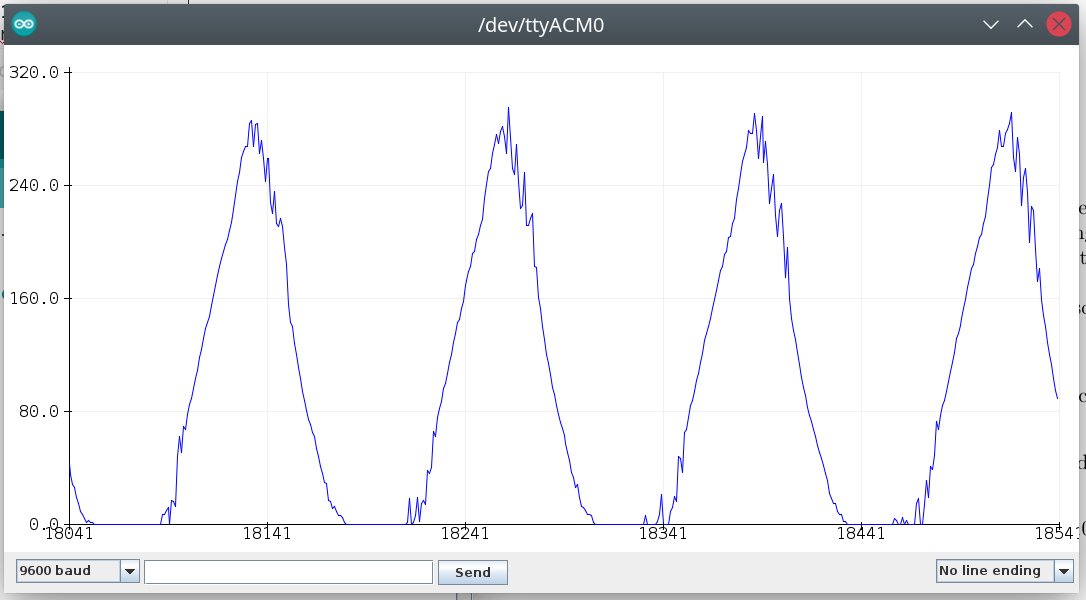
\includegraphics[width=0.8\textwidth]{Dispositivo_files/serialdebug.png}
	\caption{Esempio di output su \textit{serial monitor}. (Nota: in questo esempio il sensore non era collegato, quindi il grafico mostra interferenze provenienti dall'esterno)}
	\label{fig:serialdebug}
\end{figure}

Per misurare le tempistiche di esecuzione del firmware (e in particolar modo, determinare il sample rate nelle varie modalità) non si può semplicemente fare una differenza tra timestamp e stamparla su seriale, poiché questo rallenterebbe troppo l'esecuzione a causa dei calcoli necessari e le continue chiamate a \texttt{Serial.write}, per cui la tecnica che viene implementata quando il firmware è compilato col flag \texttt{OSCILLOSCOPE\_DEBUG} è quella di generare un segnale che è \texttt{HIGH} mentre il firmware sta leggendo il sensore e \texttt{LOW} mentre sta scrivendo sulla seriale (o viceversa); collegando un oscilloscopio all'uscita di questo segnale è possibile misurarne la frequenza (e quindi il sample rate) e verificare anche la presenza di ``buchi'' nel campionamento. Con la stessa tecnica è possibile misurare i tempi di esecuzione delle ISR.\\
La generazione di questo segnale non può essere fatta utilizzando funzioni come \texttt{digitalWrite} poiché richiedono parecchi microsecondi per essere eseguite e questo invaliderebbe completamente la misura. Studiando la documentazione del microcontroller 32U4 si scopre la presenza di una funzione speciale del pin 10: quando il bit 6 del registro \texttt{PINB} viene scritto ad 1, il valore corrente di quel pin viene invertito\cite{atmega32u4_datasheet}. Scrivere il registro \texttt{PINB} richiede un singolo ciclo di clock, che corrisponde a 62ns, un ordine di grandezza inferiore ai tempi che stiamo cercando di misurare.\\
Per rendere facilmente utilizzabile questa funzione nel firmware, sono state realizzate tre macro:
\begin{itemize}
	\item \texttt{OSCILLOSCOPE\_DEBUG\_INIT()}: inizializza il pin 10 come output e con un segnale \texttt{LOW}
	\item \texttt{OSCILLOSCOPE\_DEBUG\_PULSE()}: inverte il valore del pin 10 manipolando il registro \texttt{PINB}
	\item \texttt{OSCILLOSCOPE\_DEBUG\_END()}: reimposta in pin 10 ad alta impedenza e cancella lo stato \texttt{HIGH} o \texttt{LOW}
\end{itemize}
Nella versione finale del firmware, queste macro sono usate per generare una pulsazione per ogni sample (con flag \texttt{NOBUFFER} impostato a 1) o per ogni buffer (senza flag \texttt{NOBUFFER}). In modalità con buffering, per ottenere il sample rate, la frequenza del segnale generato va moltiplicata per la dimensione del buffer (32 se il flag \texttt{MONITOR} è impostato a 1, altrimenti 21).

La figura \ref{fig:oscilloscopedebug} mostra un esempio del segnale generato da questa modalità di debugging. Il dispositivo stava operando con \texttt{NOBUFFER=1}, \texttt{MONITOR=1}, \texttt{FASTADC=1}, per un sample rate di 21000Hz. Piccole variazioni della frequenza di questo segnale sono perfettamente normali, e possono avvenire in seguito a interrupt (click automatici o esterni) o semplicemente per variazioni sul segnale di clock; non influiscono in maniera rilevante sulle misurazioni fatte dall'applicazione.

\begin{figure}[h]
	\centering
	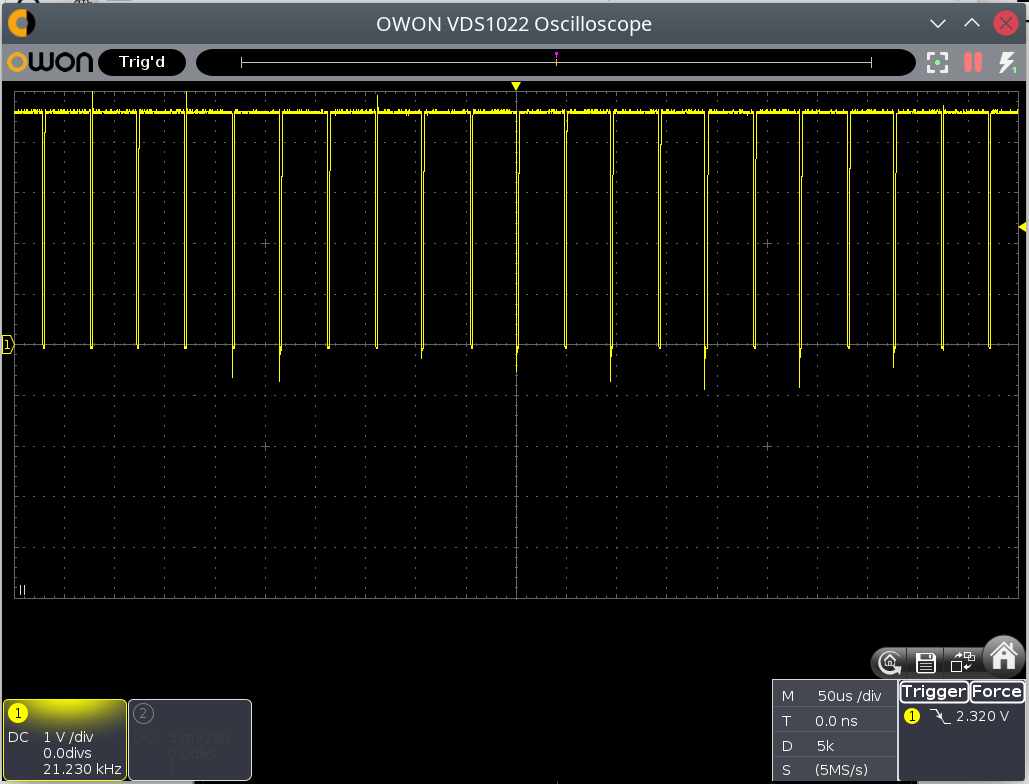
\includegraphics[width=0.8\textwidth]{Dispositivo_files/scope.png}
	\caption{Esempio di segnale generato da \texttt{OSCILLOSCOPE\_DEBUG}}
	\label{fig:oscilloscopedebug}
\end{figure}

Attenzione: le velocità di campionamento possono variare leggermente a causa degli aggiornamenti del compilatore GCC e delle librerie Arduino. Per questo motivo viene fornito un firmware precompilato in formato .hex da caricare sul dispositivo con il tool avrdude.

\section{Assemblaggio e flashing del dispositivo}
Questa sezione è una guida passo-passo per l'assemblaggio e la preparazione del dispositivo OpenLDAT.

\subsection{Assemblaggio}
Il dispositivo OpenLDAT è piuttosto semplice da assemblare, il processo richiede tra 15 e 60 minuti a seconda del livello di abilità di saldatura.

Prima di iniziare, bisogna preparare i seguenti strumenti:
\begin{itemize}
	\item Saldatore a stagno a 450°C
	\item Rotolo di stagno per saldatura, meglio se con flussante
	\item Tronchesino o strumento di taglio simile
	\item Una breadboard o altro strumento in cui tenere fermi i pin header mentre si salda
\end{itemize}

Attenzione: la qualità delle saldature influisce direttamente sulla qualità dei segnali che il dispositivo OpenLDAT sarà in grado di catturare.

Una volta preparati tutti gli strumenti, si possono preparare i materiali (figura \ref{fig:assembly_01}):
\begin{itemize}
	\item Board Sparkfun Pro Micro 5V/16MHz con header
	\item Sensore Adafruit ALS-PT19 con header
	\item PCB OpenLDAT Model 1 (stampato o fatto in casa)
	\item Resistenze (330k\si{\ohm}, 22k\si{\ohm}, 47k\si{\ohm}, 1k\si{\ohm}, 1k\si{\ohm})
	\item LED da 5mm
\end{itemize}

\paragraph{Passo 1} Saldare gli header sulla board Sparkfun Pro Micro, in modo che la parte in plastica e la parte lugna dei pin sia sotto alla board. Per tenere i pin fermi e dritti mentre si salda, è utile infilarli in una breadboard o in un \textit{soldering jig} apposito, come in figura \ref{fig:assembly_02}.

\paragraph{Passo 2} Saldare gli header sul piccolo PCB del sensore ALS-PT19, in modo che la parte in plastica e la parte lunga dei pin sia sotto al PCB e il sensore sia sopra, come in figura \ref{fig:assembly_03}. Poiché il PCB è molto piccolo, bisogna prestare attenzione a non scaldarlo troppo col saldatore, altrimenti il sensore potrebbe danneggiarsi.

\paragraph{Passo 3} Sulla parte posteriore del PCB OpenLDAT (quella dove ci sono le piste), posizionare le resistenze nelle posizioni corrette, piegando le gambette per tenerle ferme come in figura \ref{fig:assembly_04}, dopodiché saldarle e tagliare l'eccesso con il tronchesino, come in figura \ref{fig:assembly_05}.\\
\textbf{Attenzione: se le resistenze non sono in posizione corretta, i livelli di gain del sensore saranno totalmente diversi da quelli che si aspetta l'applicazione, e questa produrrà risultati errati.}\\
Il seguente elenco riassume le resistenze che devono essere saldate sul dispositivo, con i relativi valori e codici dei colori:
\begin{itemize}
	\item R1: 1k\si{\ohm} (Marrone-Nero-Rosso)
	\item R2: 1M\si{\ohm} (Marrone-Nero-Verde)
	\item R3: 330k\si{\ohm} (Arancio-Arancio-Giallo)
	\item R4: 22k\si{\ohm} (Rosso-Rosso-Arancio)
	\item R5: 47k\si{\ohm} (Giallo-Viola-Arancio)
\end{itemize}

\paragraph{Passo 4} Posizionare il sensore ALS-PT19 sulla parte posteriore del PCB OpenLDAT come in figura \ref{fig:assembly_06} e saldarlo avendo cura di tenerlo in posizione parallela al PCB, dopodiché, usando il tronchesino, rimuovere i pin in eccesso come in figura \ref{fig:assembly_07}.

\paragraph{Passo 5} Sulla parte frontale del PCB OpenLDAT, posizionare la board Sparkfun Pro Micro con il connettore USB dallo stesso lato del sensore ALS-PT19 e posizionare il LED prestando attenzione alla polarità, piegando le gambette per tenerlo fermo, come in figura \ref{fig:assembly_08}, dopodiché saldare il tutto e usando il tronchesino, rimuovere i pin in eccesso dalla parte posteriore del PCB, come in figura \ref{fig:assembly_09}.

\paragraph{Passo 6} Posizionare i due pin header per il collegamento del pulsante esterno sulla parte frontale del PCB OpenLDAT e saldarli come in figura \ref{fig:assembly_10}. A questo punto il dispositivo è completo.

\paragraph{Passo 7} Ora è possibile inserire il dispositivo all'interno del case stampato in 3D mostrato in figura \ref{fig:assembly_11}. Prima di iniziare, opzionalmente, è possibile eseguire alcune migliorie opzionali al case:
\begin{itemize}
	\item È possibile posizionare un vetrino da microscopio 22x22mm nell'apposito incavo sul fondo della base, per proteggere il sensore da tocchi accidentali. Per tenere fermo il vetrino si consiglia di usare della resina epossidica, facendo attenzione a non sporcare il vetro posizionandola (figura \ref{fig:assembly_12})
	\item Sulla parte inferiore della base, dove il dispositivo viene appoggiato sul display da testare, è possibile posizionare dei feltrini o uno strato di carta adesiva vellutata, avendo cura di non ostruire neanche parzialmente il sensore ed evitando di creare potenziali infiltrazioni di luce (figura \ref{fig:assembly_13})
\end{itemize}

\paragraph{Passo 8} Inserire il PCB assemblato all'interno del case bloccandolo nei quattro incastri appositi, con il sensore rivolto verso il basso. Si consiglia di inserire prima la parte con il connettore USB e poi premere la parte tra il connettore del pulsante esterno e il LED per completare l'incastro, come mostrato nelle immagini in figura \ref{fig:assembly_14}.\\
Per via delle tolleranze di produzione del PCB e del case, l'incastro potrebbe non essere perfetto:\begin{itemize}
	\item Se il PCB sforza troppo per entrare, si può utilizzare della carta vetrata per levigare i bordi del PCB, prestando la massima attenzione a non danneggiare il PCB o i componenti saldati su di esso
	\item Se il PCB entra ma esce troppo facilmente dall'incastro, si può usare della colla a caldo per tenerlo fermo, oppure scaldare leggermente le alette del case per restringere il PLA del case
\end{itemize}

\paragraph{Passo 9} Incastrare il diffusore opzionale che copre il LED nell'apposito foro sul coperchio come in figura \ref{fig:assembly_16}. Se l'incastro non è perfetto, si può usare della colla a caldo per tenerlo fermo.

\paragraph{Passo 10} Chiudere il dispositivo incastrando il coperchio nelle guide laterali. Per via delle tolleranze di stampa del case, l'incastro potrebbe non essere perfetto:\begin{itemize}
	\item Se il coperchio sforza troppo e non entra nelle guide, si può utilizzare della carta vetrata per levigare leggermente le alette che devono entrare nelle guide
	\item Se il coperchio entra ma esce facilmente dall'incastro, o se si vuole una garanzia in più che resti chiuso, si può posizionare una goccia di colla a caldo sulle due guide e poi incastrare il coperchio mentre è ancora calda
\end{itemize}

L'assemblaggio è ora completo e il dispositivo è pronto per ricevere il firmware.

\begin{figure}[H]
	\centering
	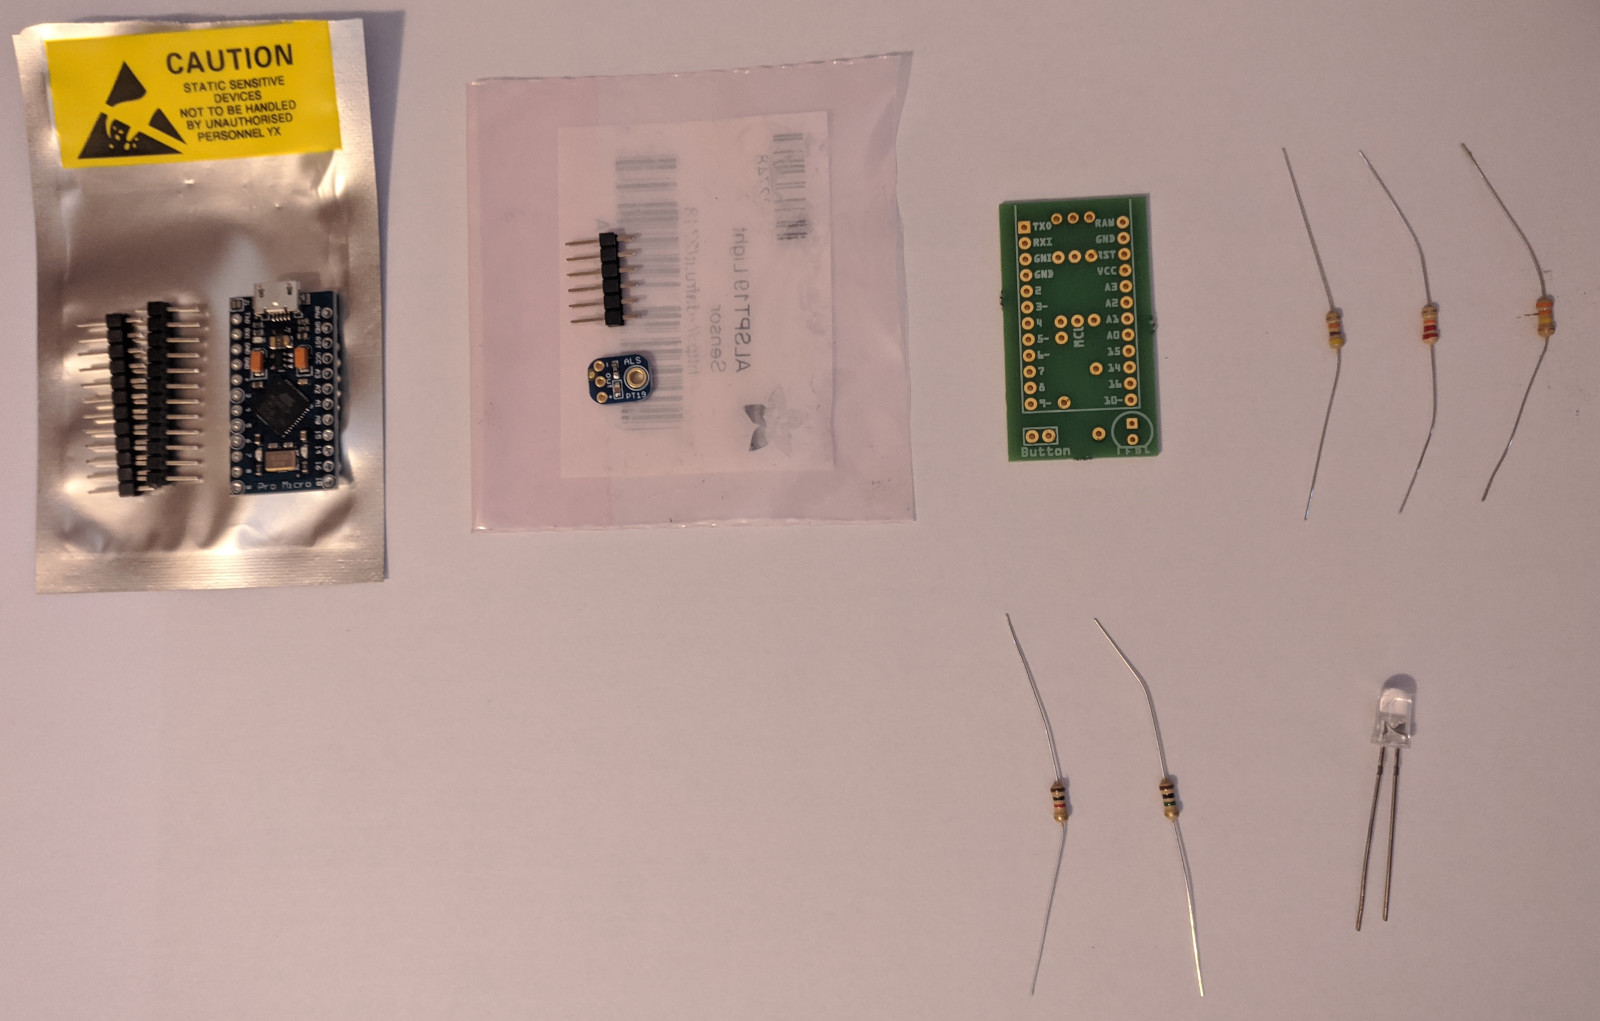
\includegraphics[width=\textwidth]{Dispositivo_files/assembly_01.jpg}
	\caption{Materiali necessari per costruire il dispositivo OpenLDAT}
	\label{fig:assembly_01}
\end{figure}

\begin{figure}[H]
	\centering
	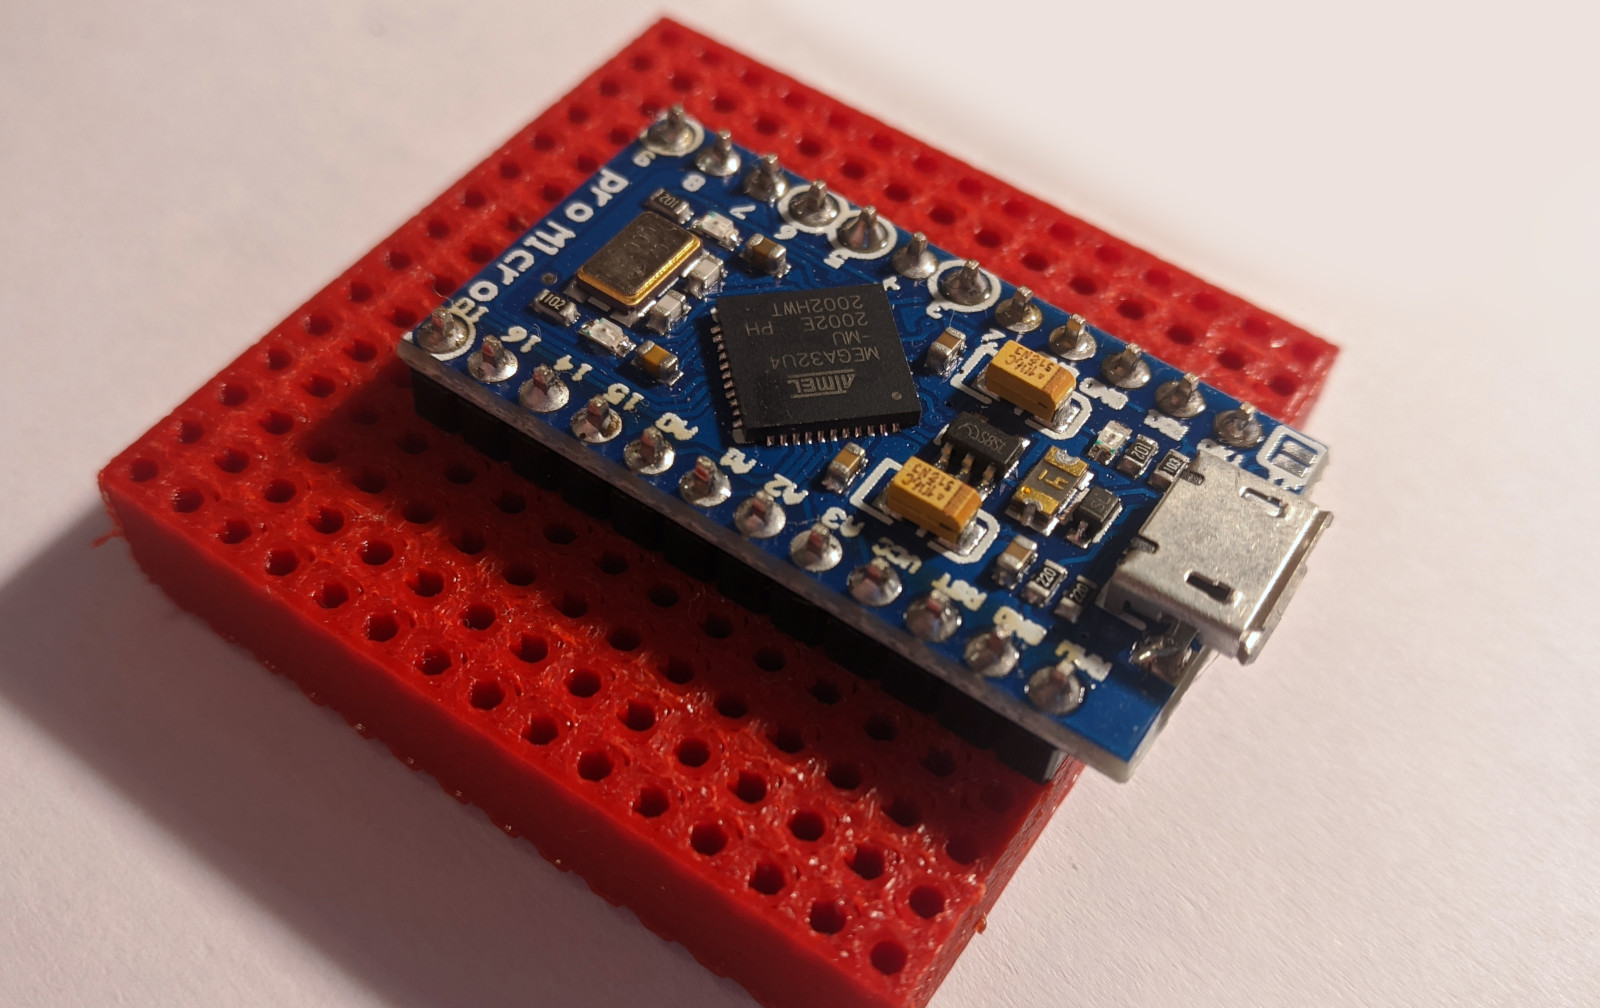
\includegraphics[width=\textwidth]{Dispositivo_files/assembly_02.jpg}
	\caption{Preparazione della board Sparkfun Pro Micro}
	\label{fig:assembly_02}
\end{figure}

\begin{figure}[H]
	\centering
	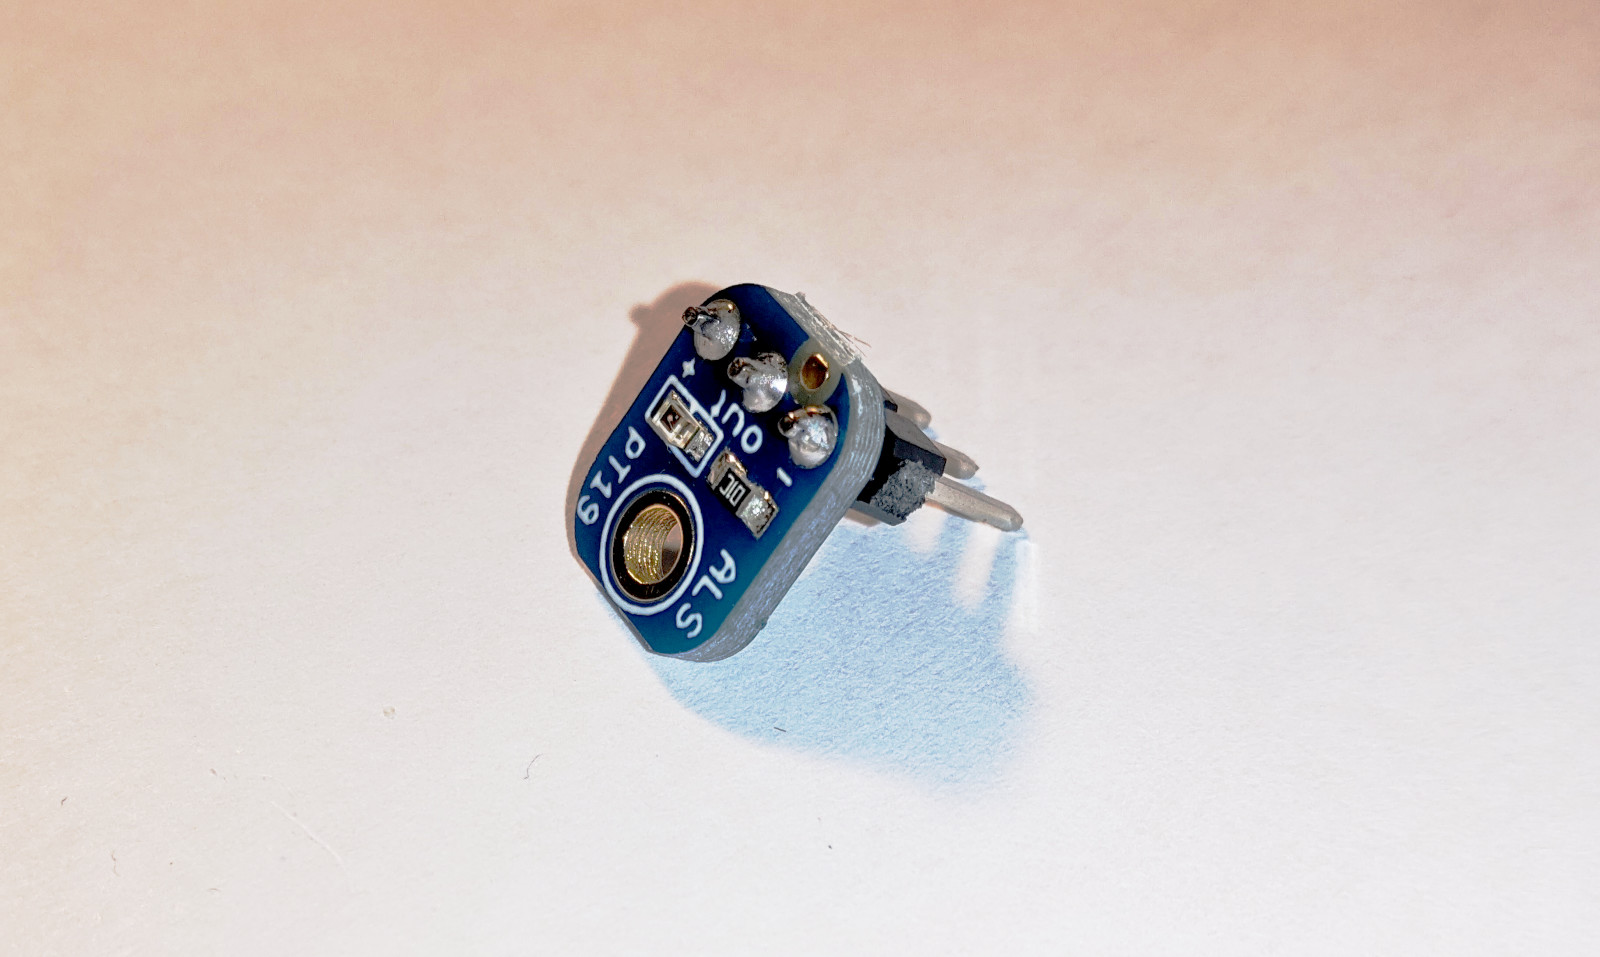
\includegraphics[width=\textwidth]{Dispositivo_files/assembly_03.jpg}
	\caption{Preparazione del sensore ALS-PT19}
	\label{fig:assembly_03}
\end{figure}

\begin{figure}[H]
	\centering
	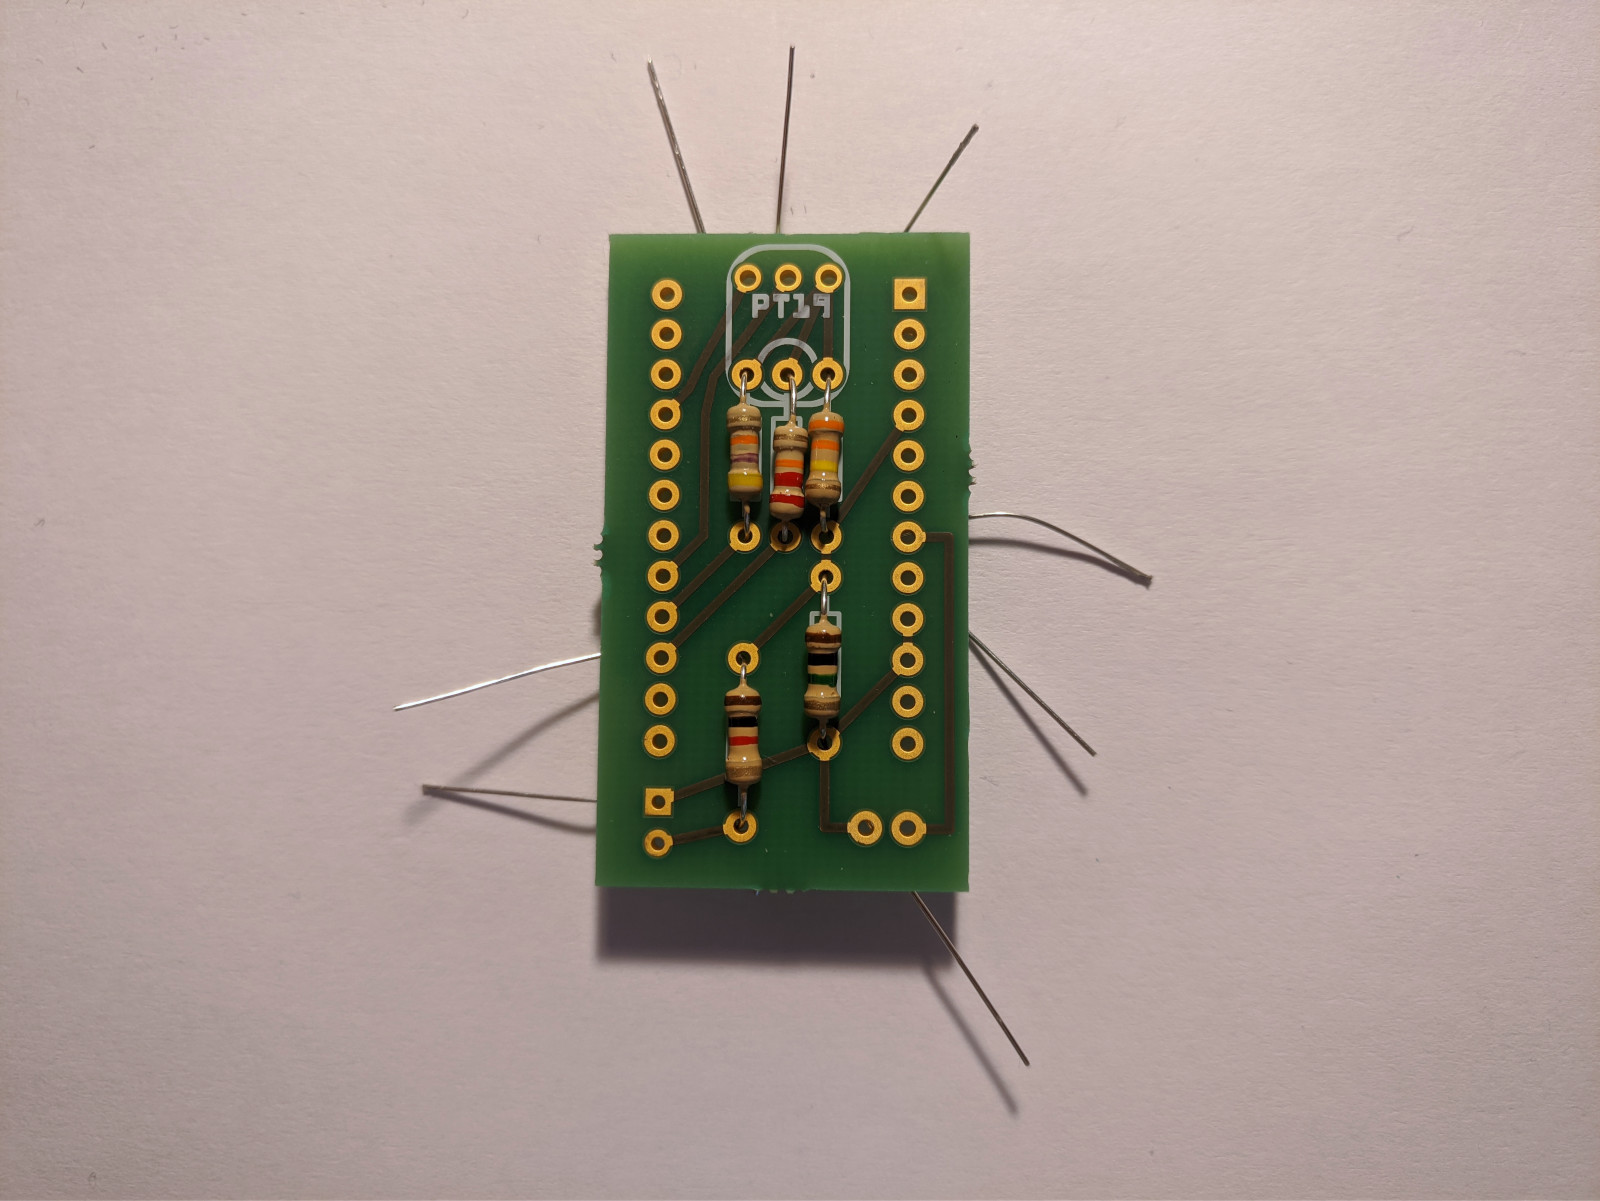
\includegraphics[width=\textwidth]{Dispositivo_files/assembly_04.jpg}
	\caption{Posizionamento delle resistenze}
	\label{fig:assembly_04}
\end{figure}

\begin{figure}[H]
	\centering
	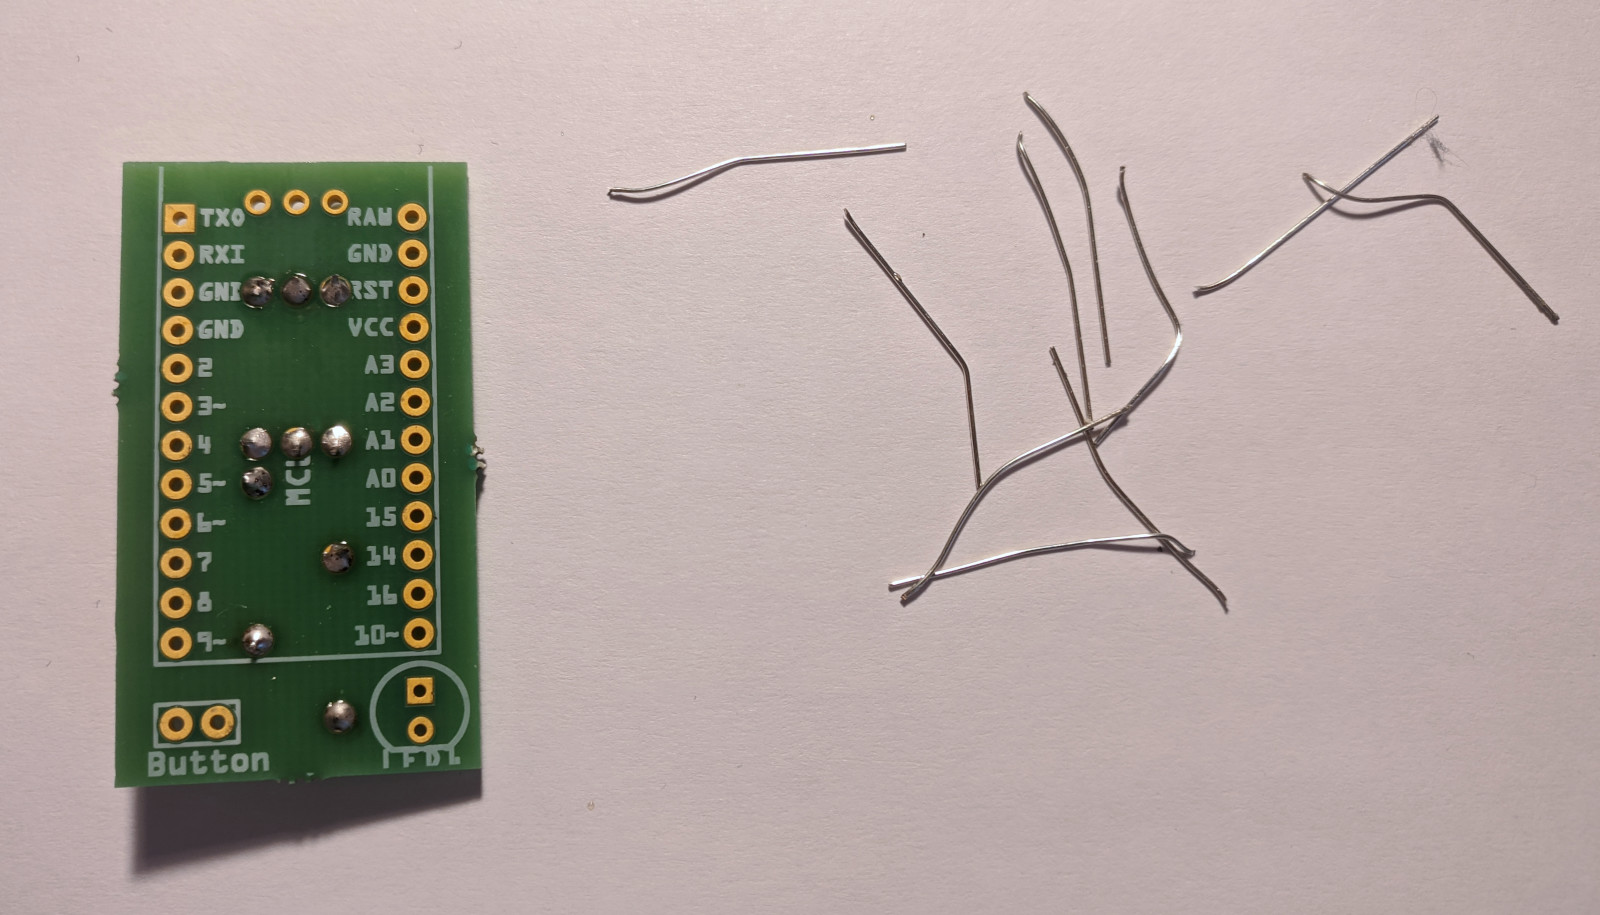
\includegraphics[width=\textwidth]{Dispositivo_files/assembly_05.jpg}
	\caption{Resistenze saldate e accorciate}
	\label{fig:assembly_05}
\end{figure}

\begin{figure}[H]
	\centering
	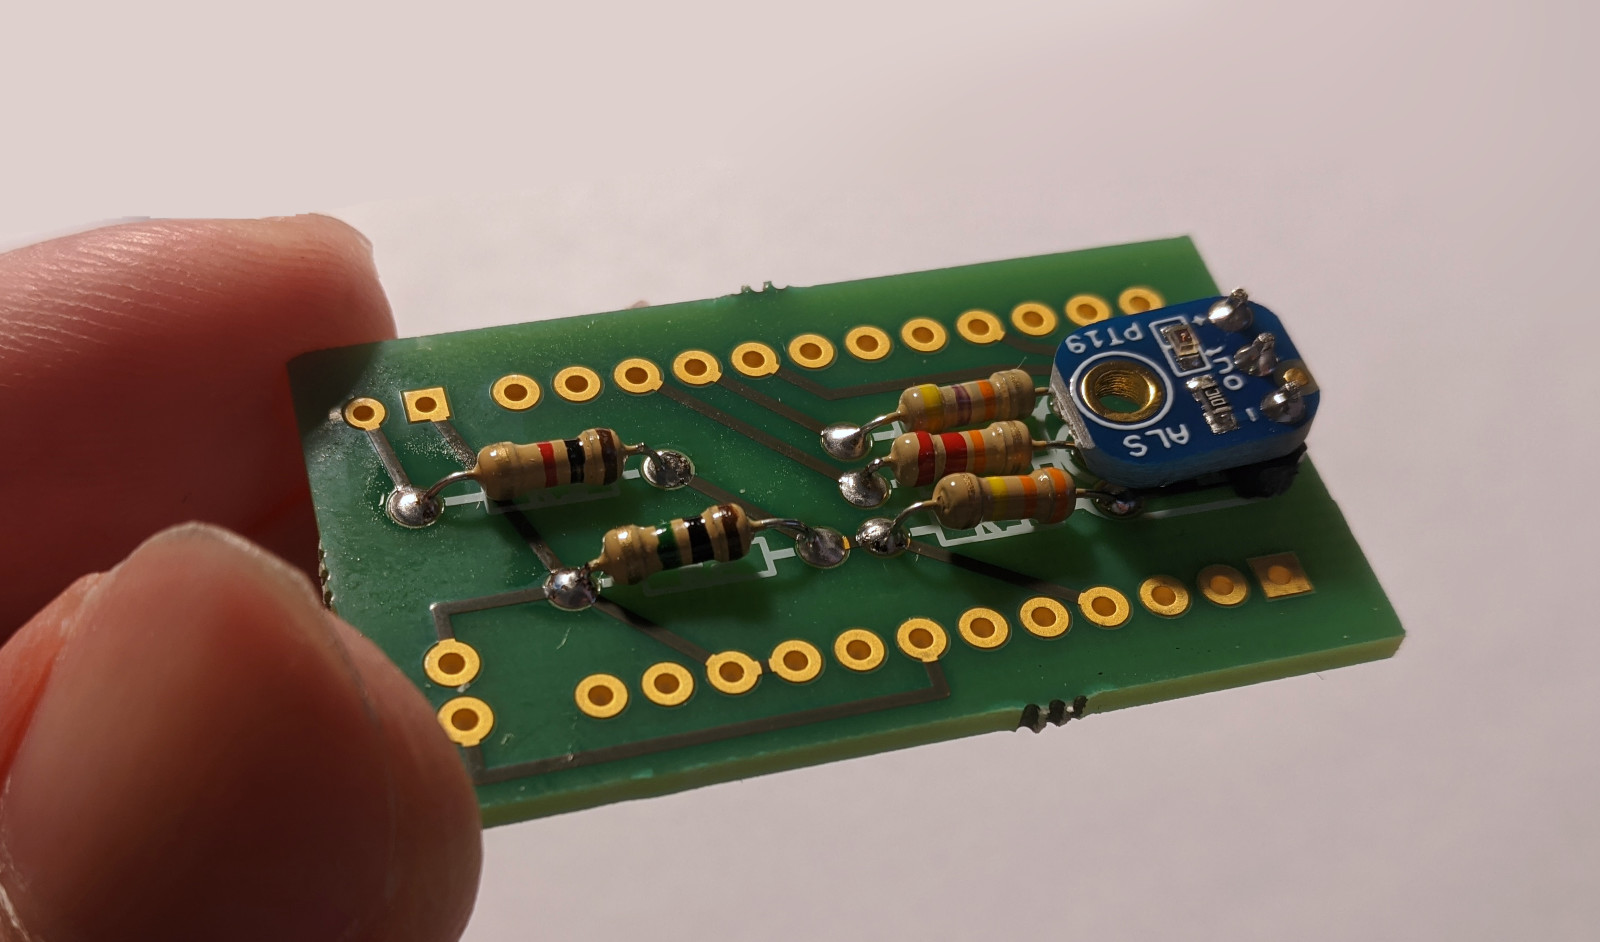
\includegraphics[width=\textwidth]{Dispositivo_files/assembly_06.jpg}
	\caption{Posizionamento del sensore ALS-PT19}
	\label{fig:assembly_06}
\end{figure}

\begin{figure}[H]
	\centering
	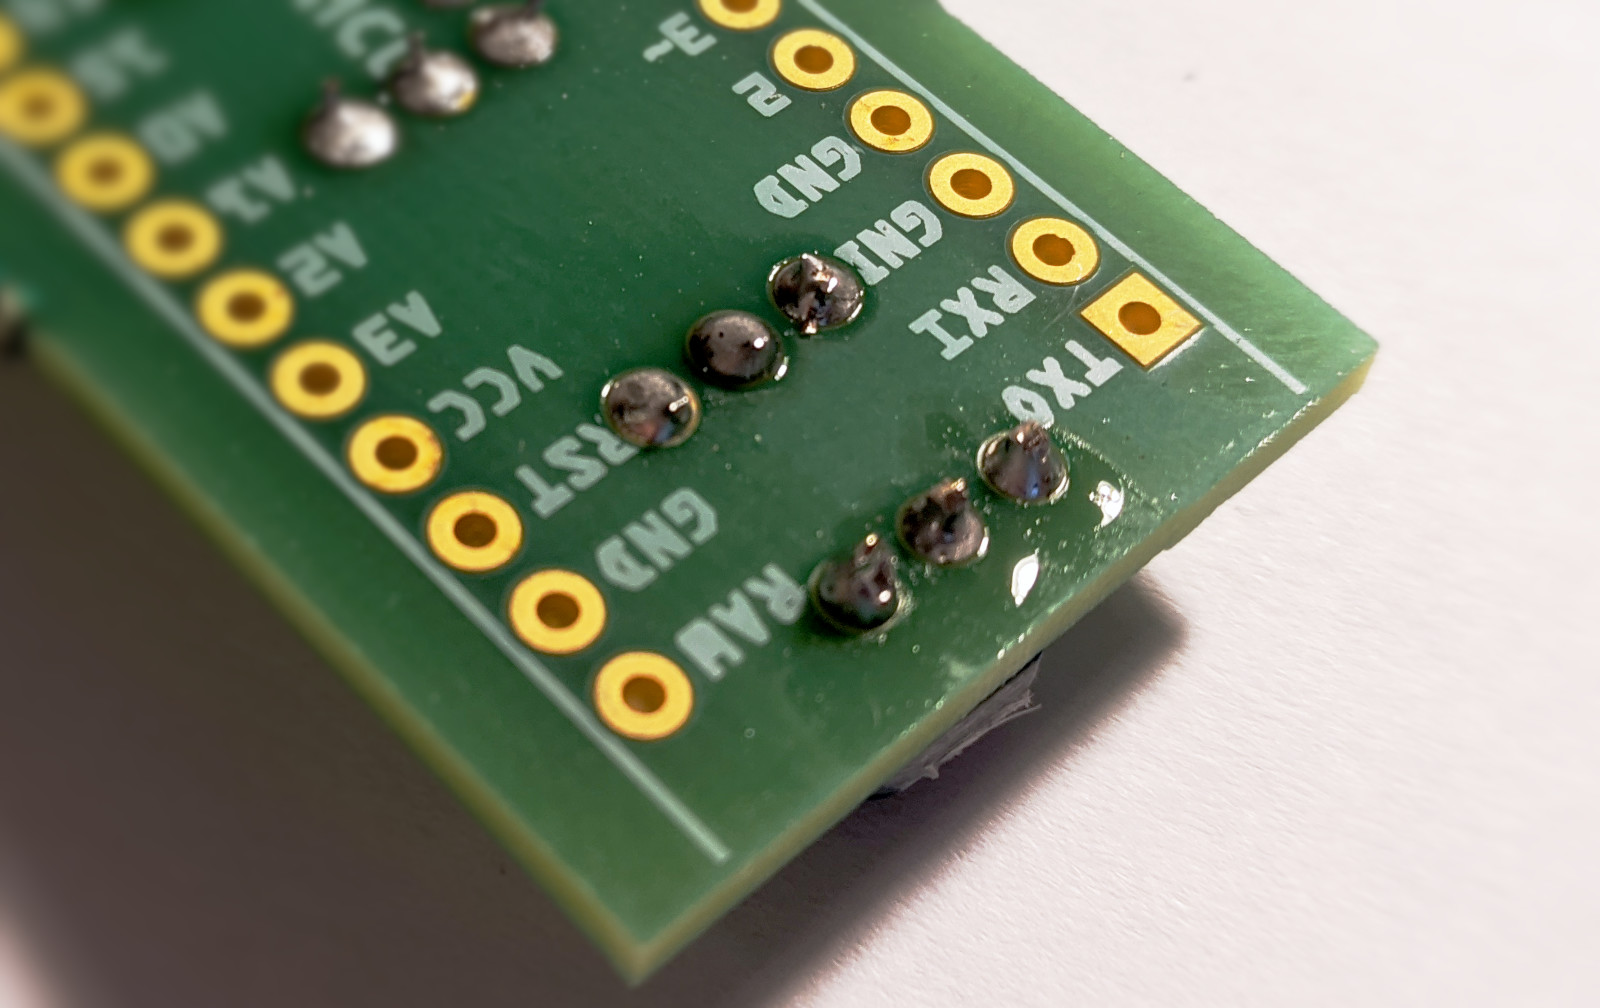
\includegraphics[width=\textwidth]{Dispositivo_files/assembly_07.jpg}
	\caption{Sensore saldato e pin accorciati}
	\label{fig:assembly_07}
\end{figure}

\begin{figure}[H]
	\centering
	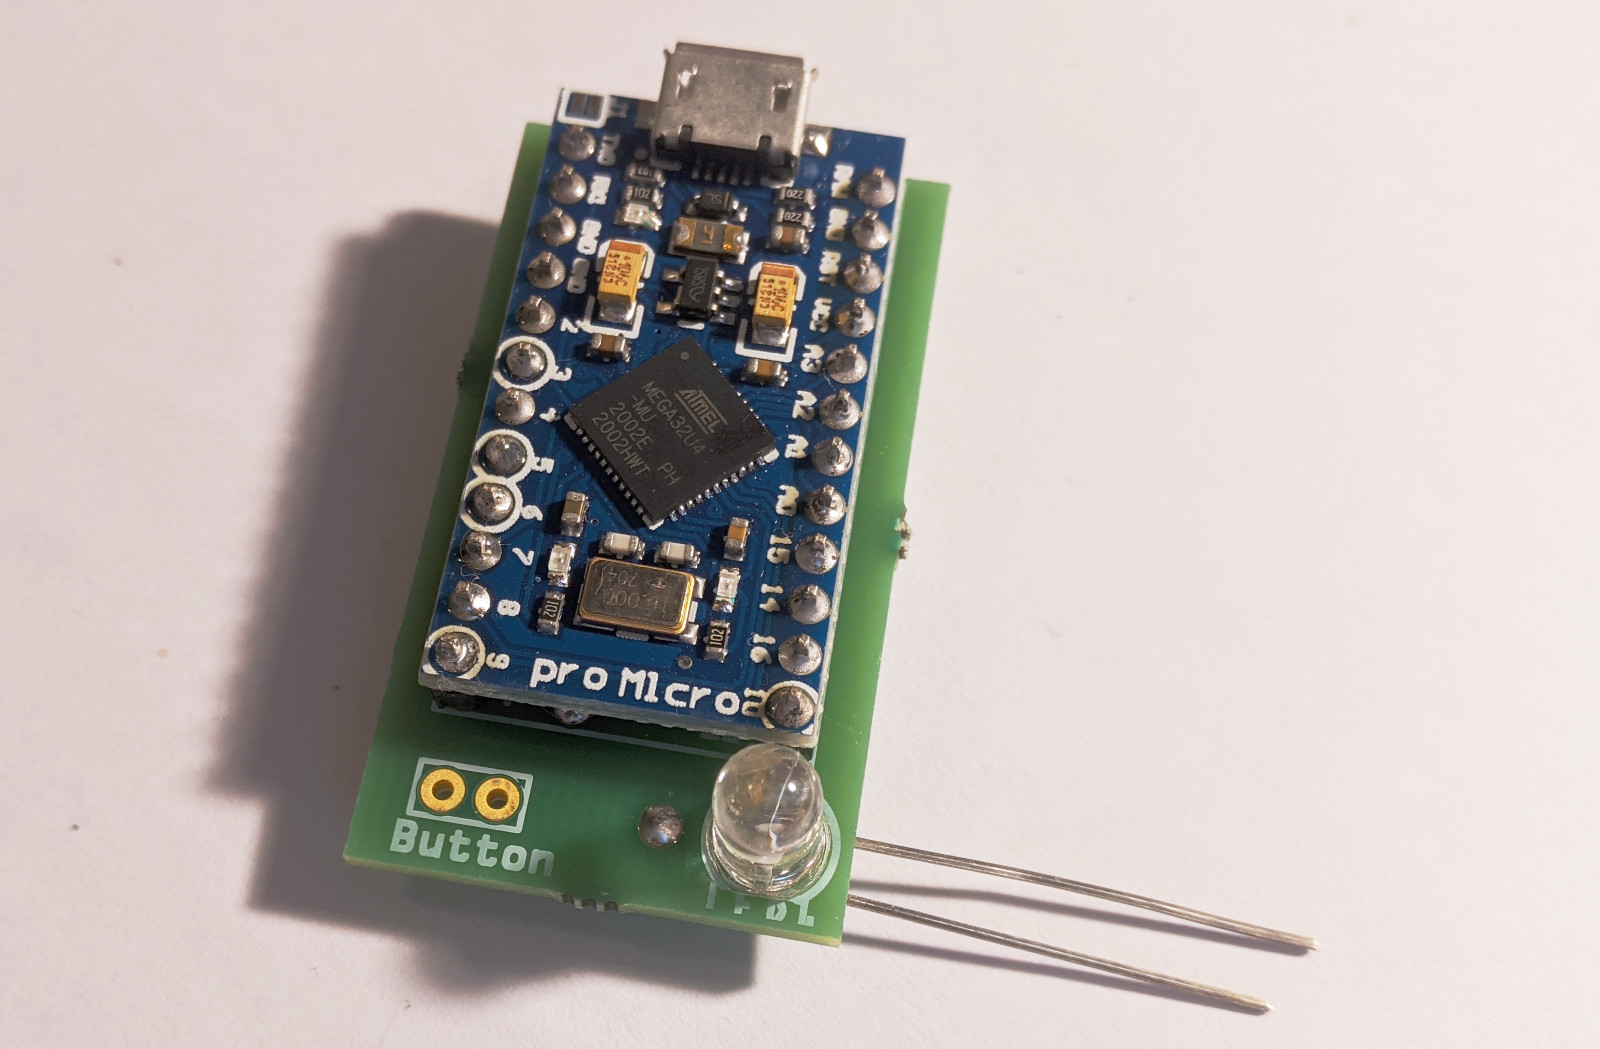
\includegraphics[width=\textwidth]{Dispositivo_files/assembly_08.jpg}
	\caption{Posizionamento dello Sparkfun Pro Micro e del LED}
	\label{fig:assembly_08}
\end{figure}

\begin{figure}[H]
	\centering
	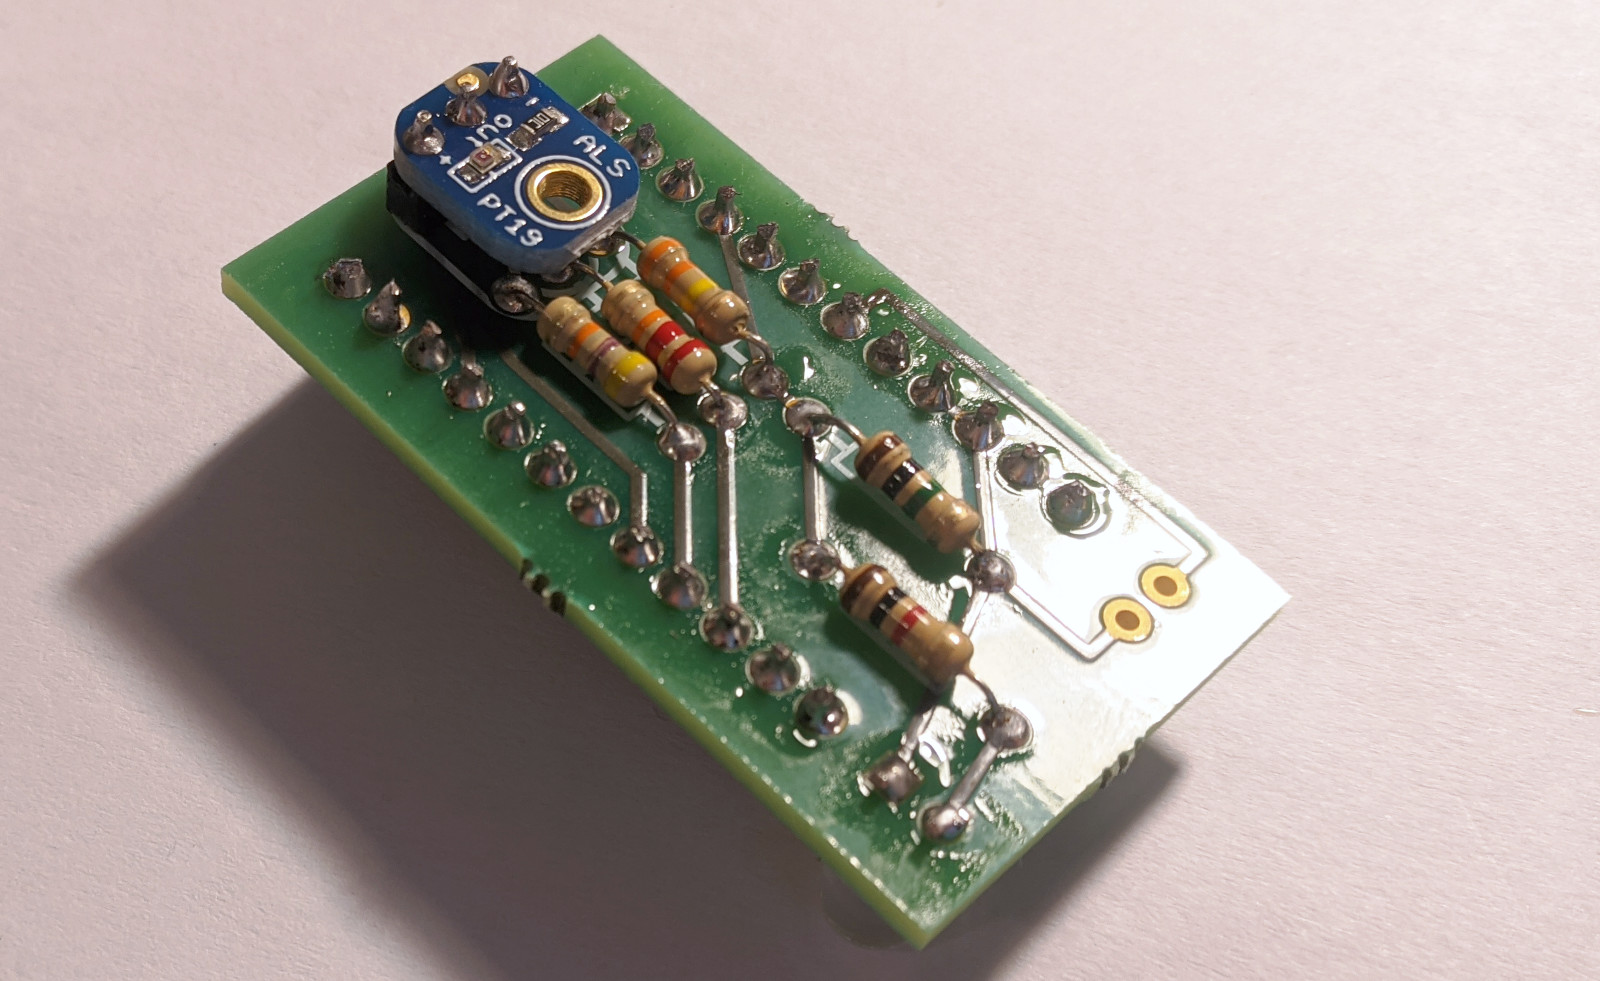
\includegraphics[width=\textwidth]{Dispositivo_files/assembly_09.jpg}
	\caption{Board e LED saldati e pin accorciati}
	\label{fig:assembly_09}
\end{figure}

\begin{figure}[H]
	\centering
	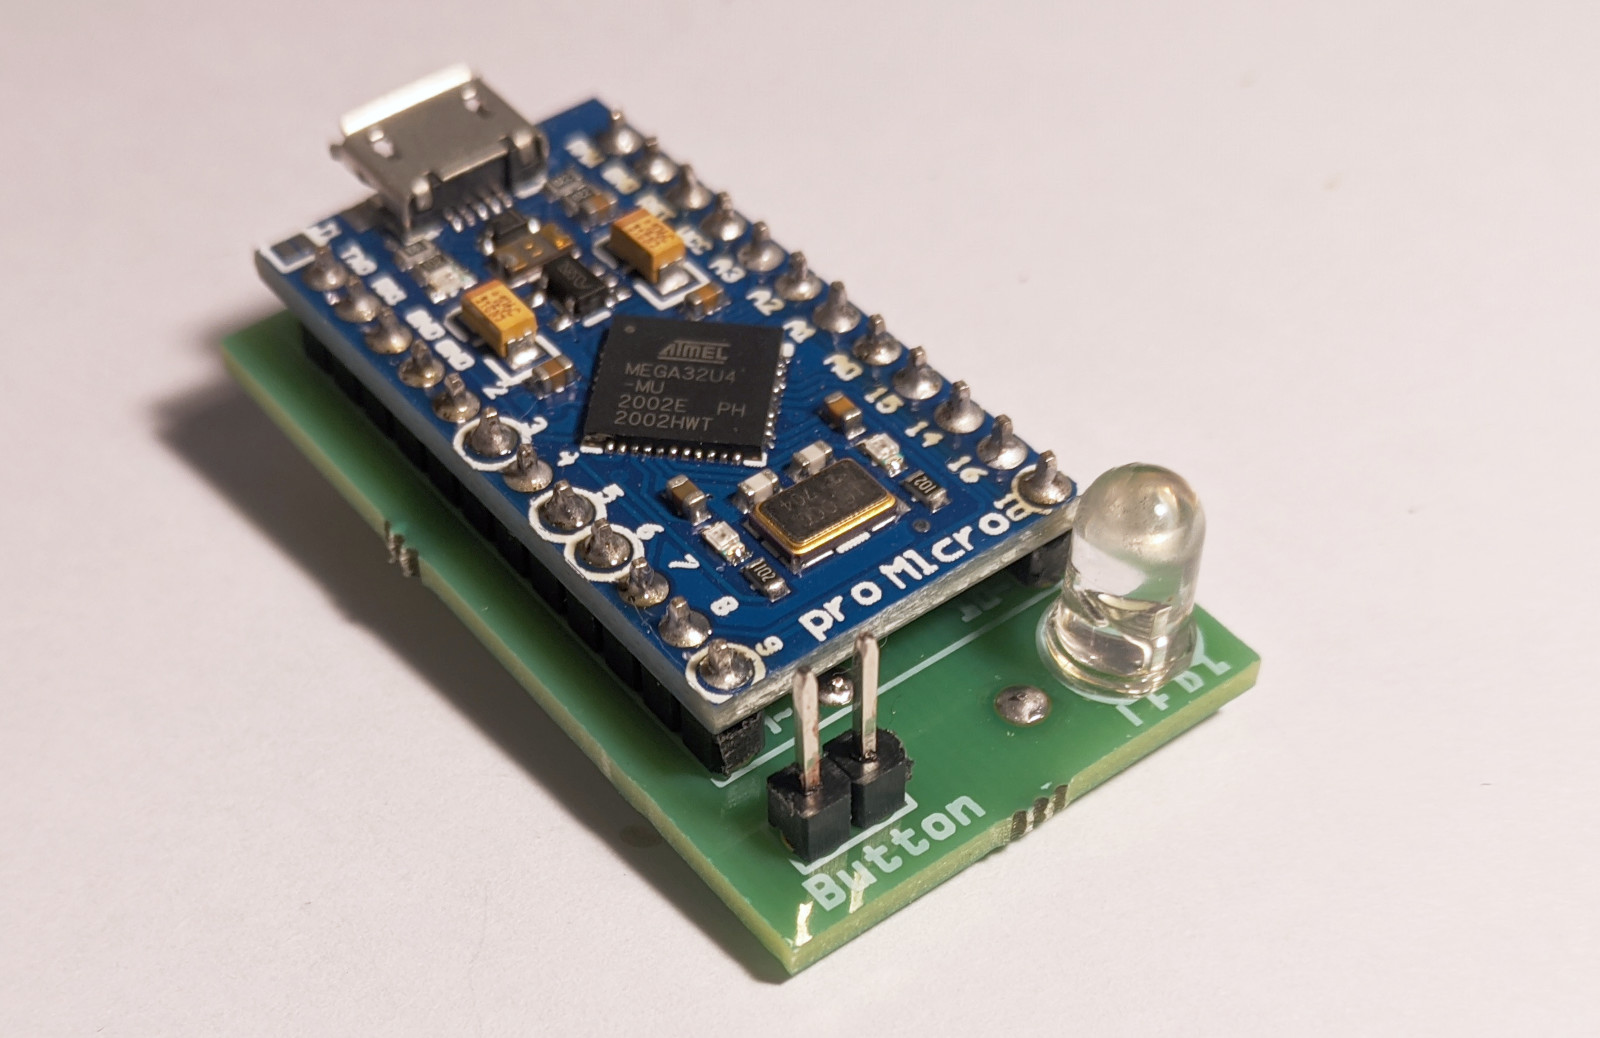
\includegraphics[width=\textwidth]{Dispositivo_files/assembly_10.jpg}
	\caption{Assemblaggio del dispositivo completato}
	\label{fig:assembly_10}
\end{figure}

\begin{figure}[H]
	\centering
	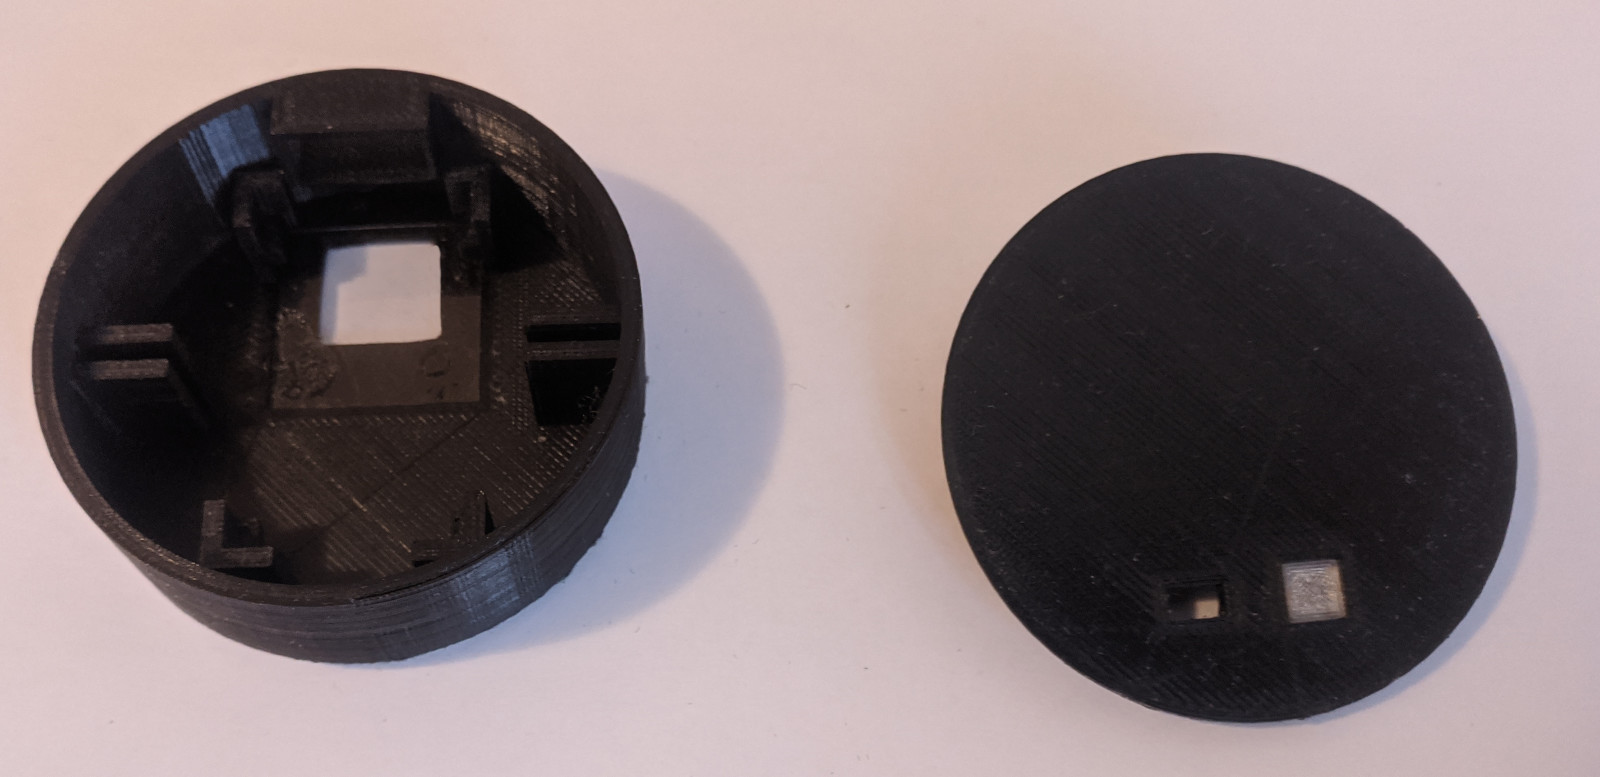
\includegraphics[width=\textwidth]{Dispositivo_files/assembly_11.jpg}
	\caption{Parti del case OpenLDAT}
	\label{fig:assembly_11}
\end{figure}

\begin{figure}[H]
	\centering
	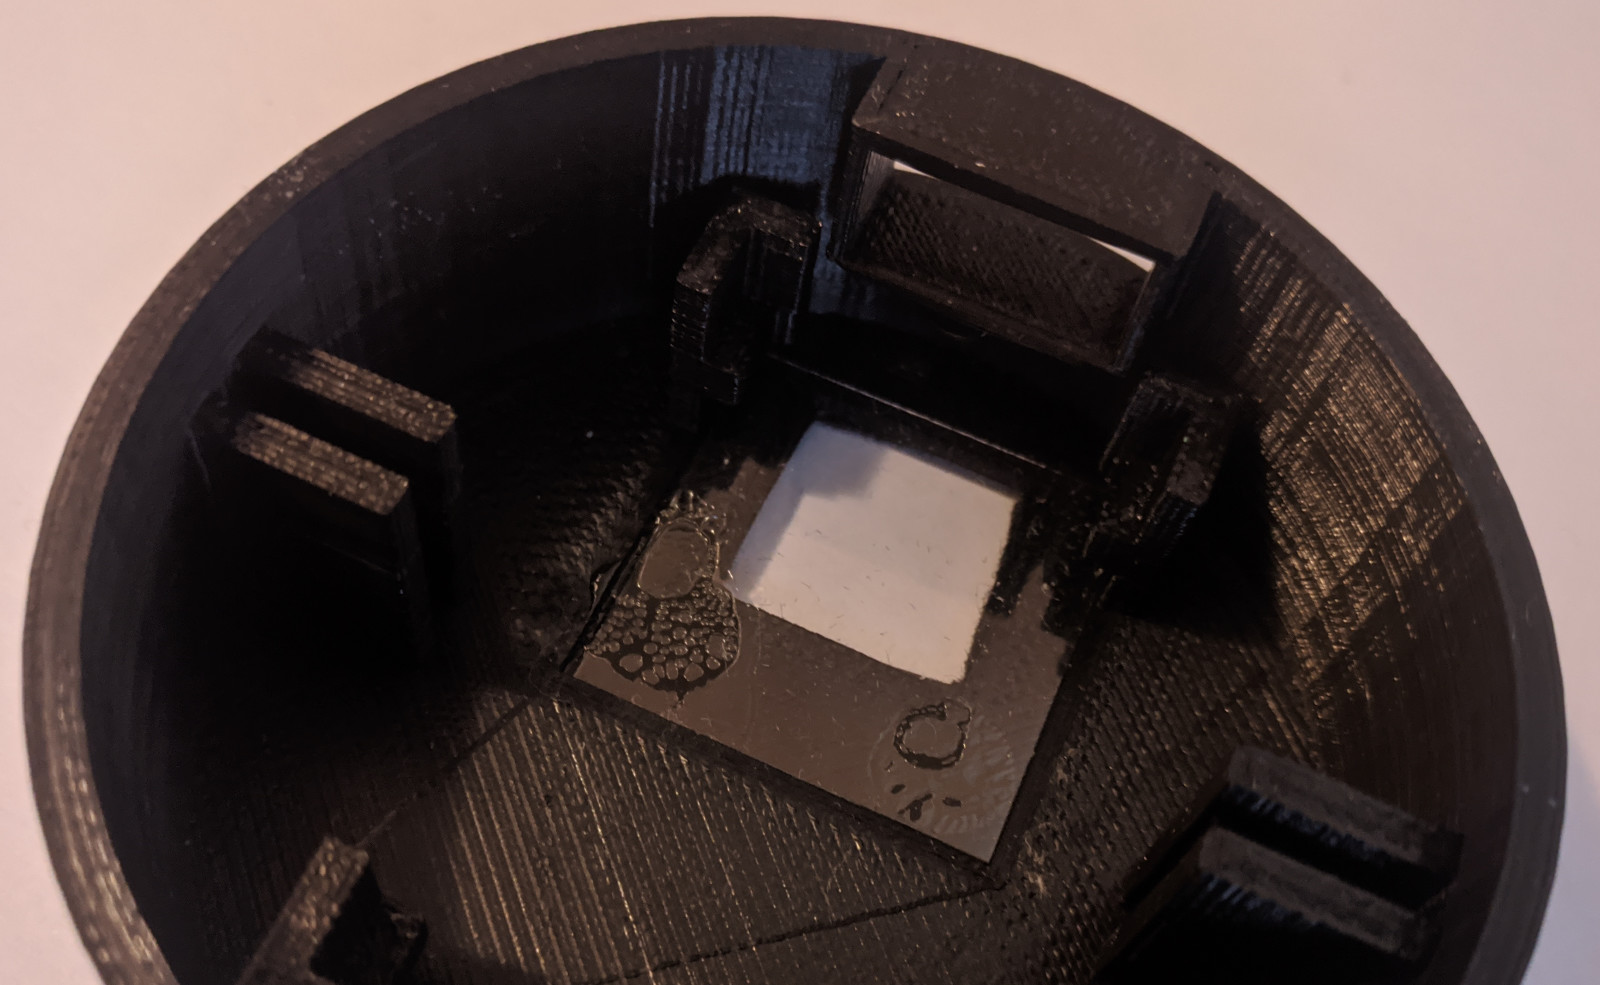
\includegraphics[width=\textwidth]{Dispositivo_files/assembly_12.jpg}
	\caption{Posizionamento del vetrino opzionale per proteggere il sensore}
	\label{fig:assembly_12}
\end{figure}

\begin{figure}[H]
	\centering
	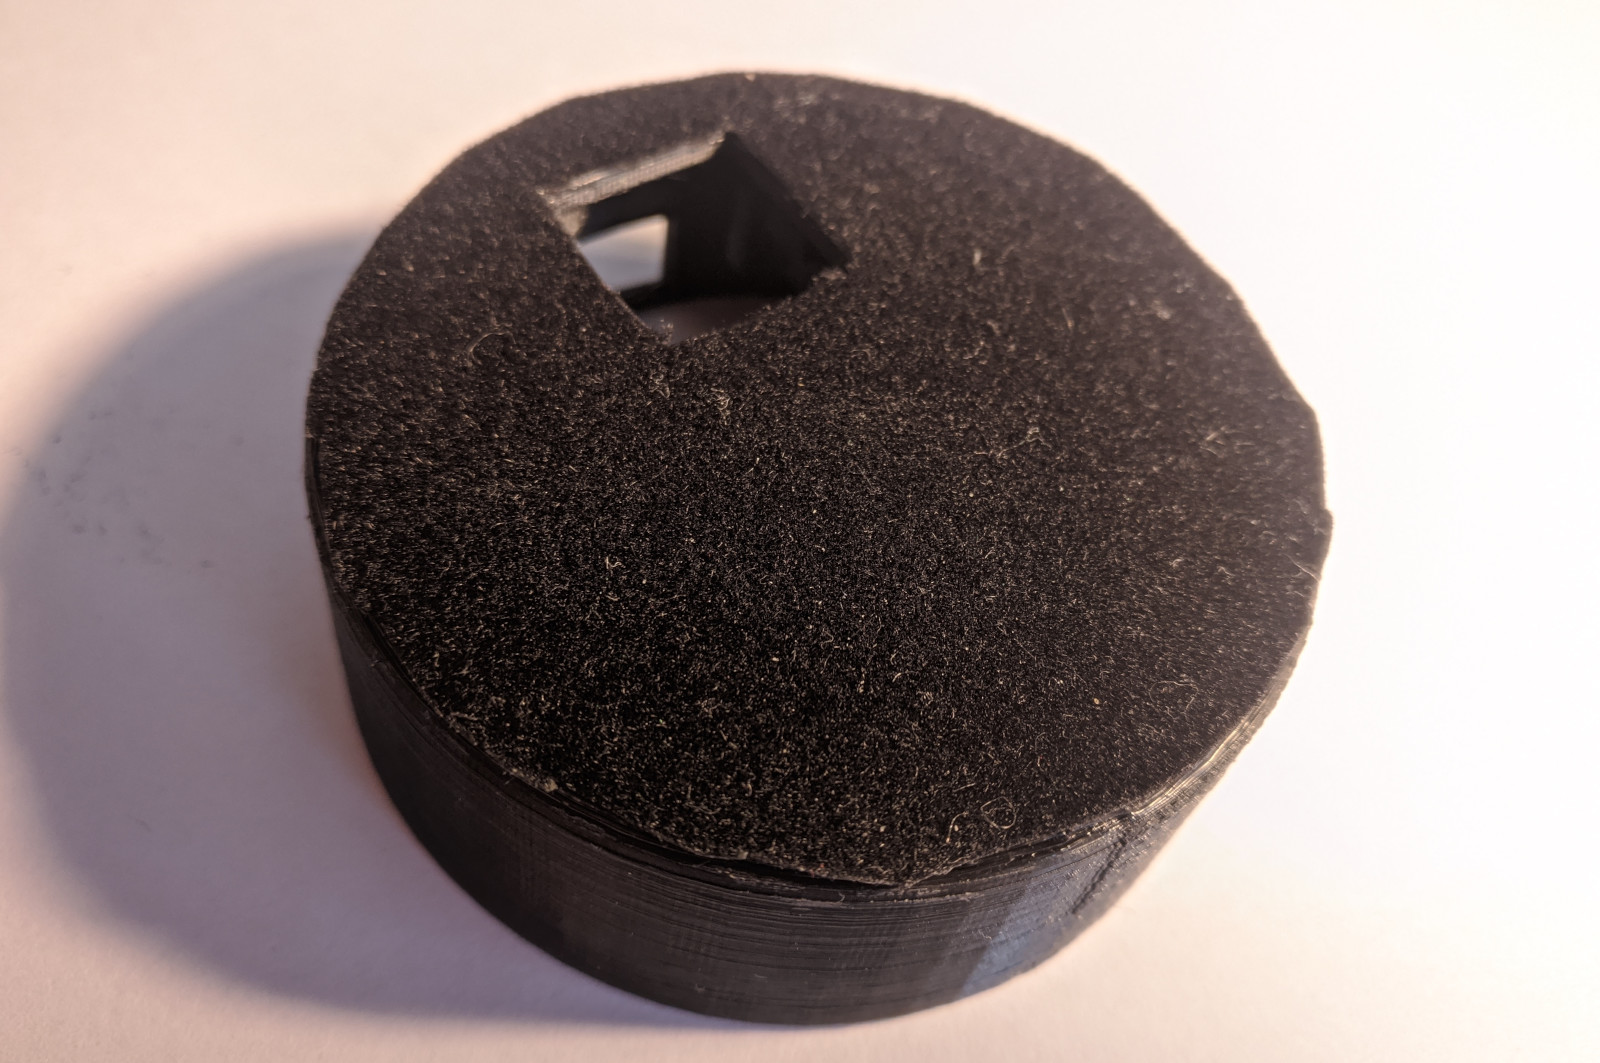
\includegraphics[width=\textwidth]{Dispositivo_files/assembly_13.jpg}
	\caption{Carta adesiva vellutata per proteggere il display testato da graffi accidentali}
	\label{fig:assembly_13}
\end{figure}

\begin{figure}[H]
	\centering
	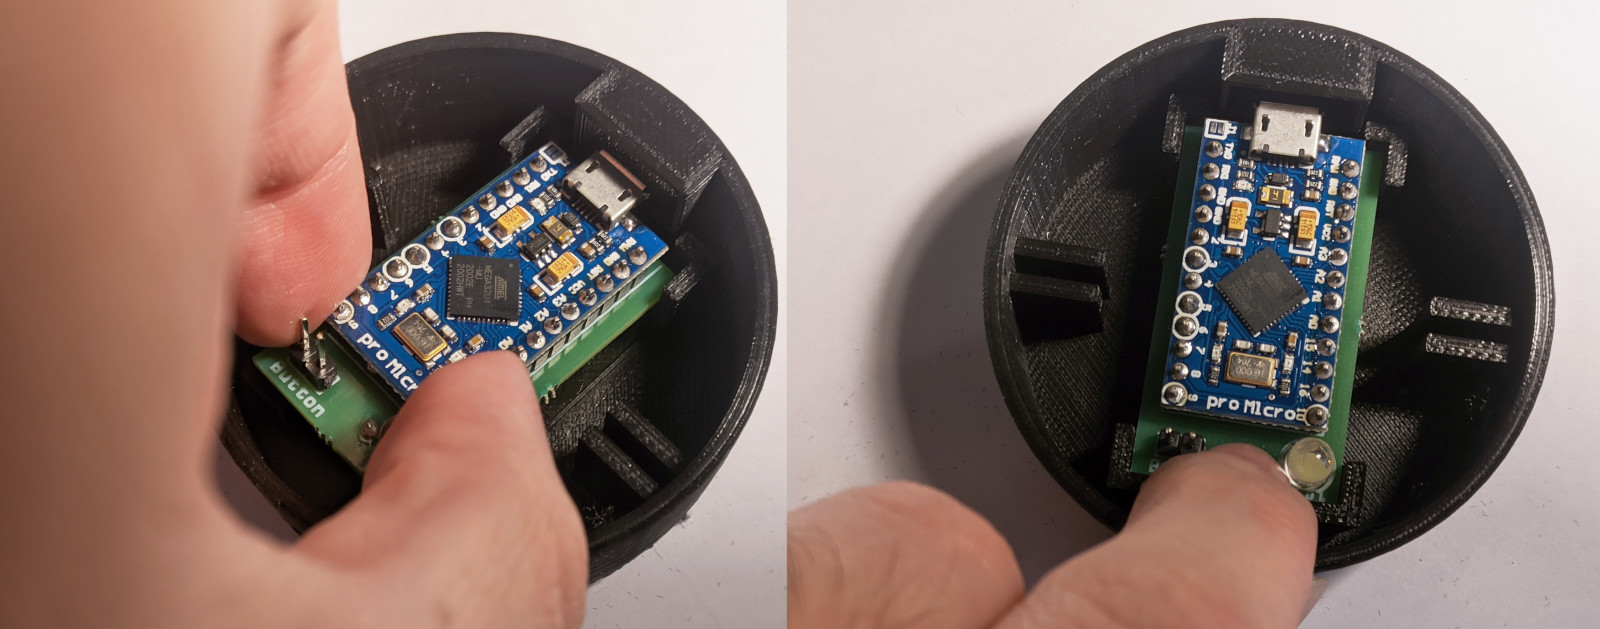
\includegraphics[width=\textwidth]{Dispositivo_files/assembly_14.jpg}
	\caption{Inserimento del PCB nel case}
	\label{fig:assembly_14}
\end{figure}

\begin{figure}[H]
	\centering
	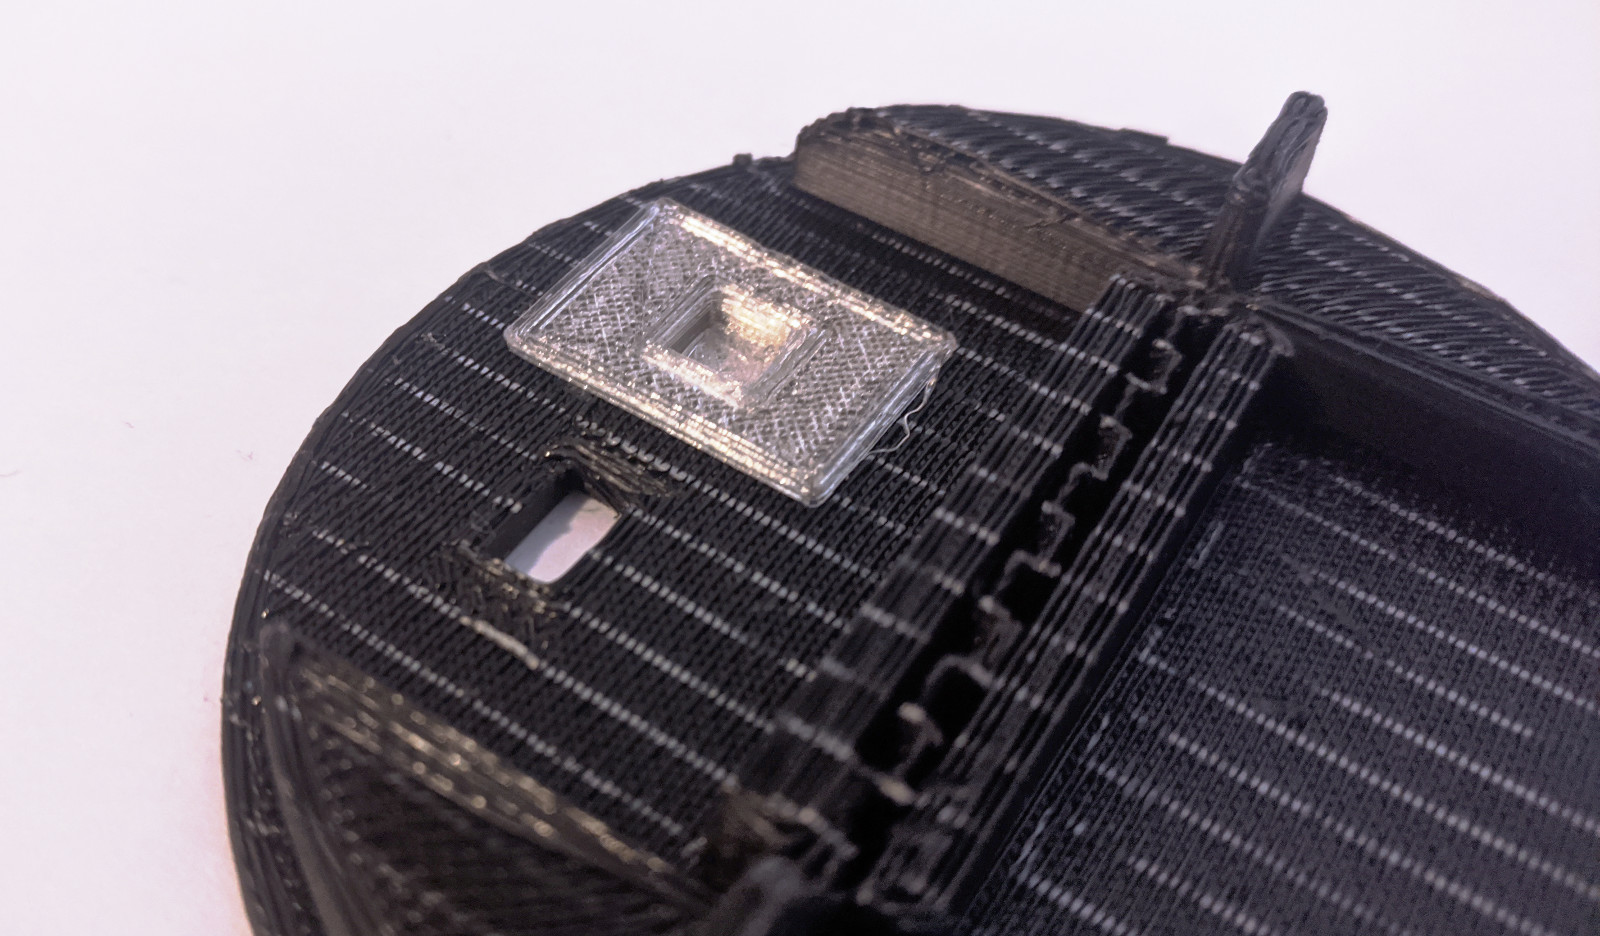
\includegraphics[width=\textwidth]{Dispositivo_files/assembly_16.jpg}
	\caption{Diffusore per il LED montato sul coperchio}
	\label{fig:assembly_16}
\end{figure}

\begin{figure}[H]
	\centering
	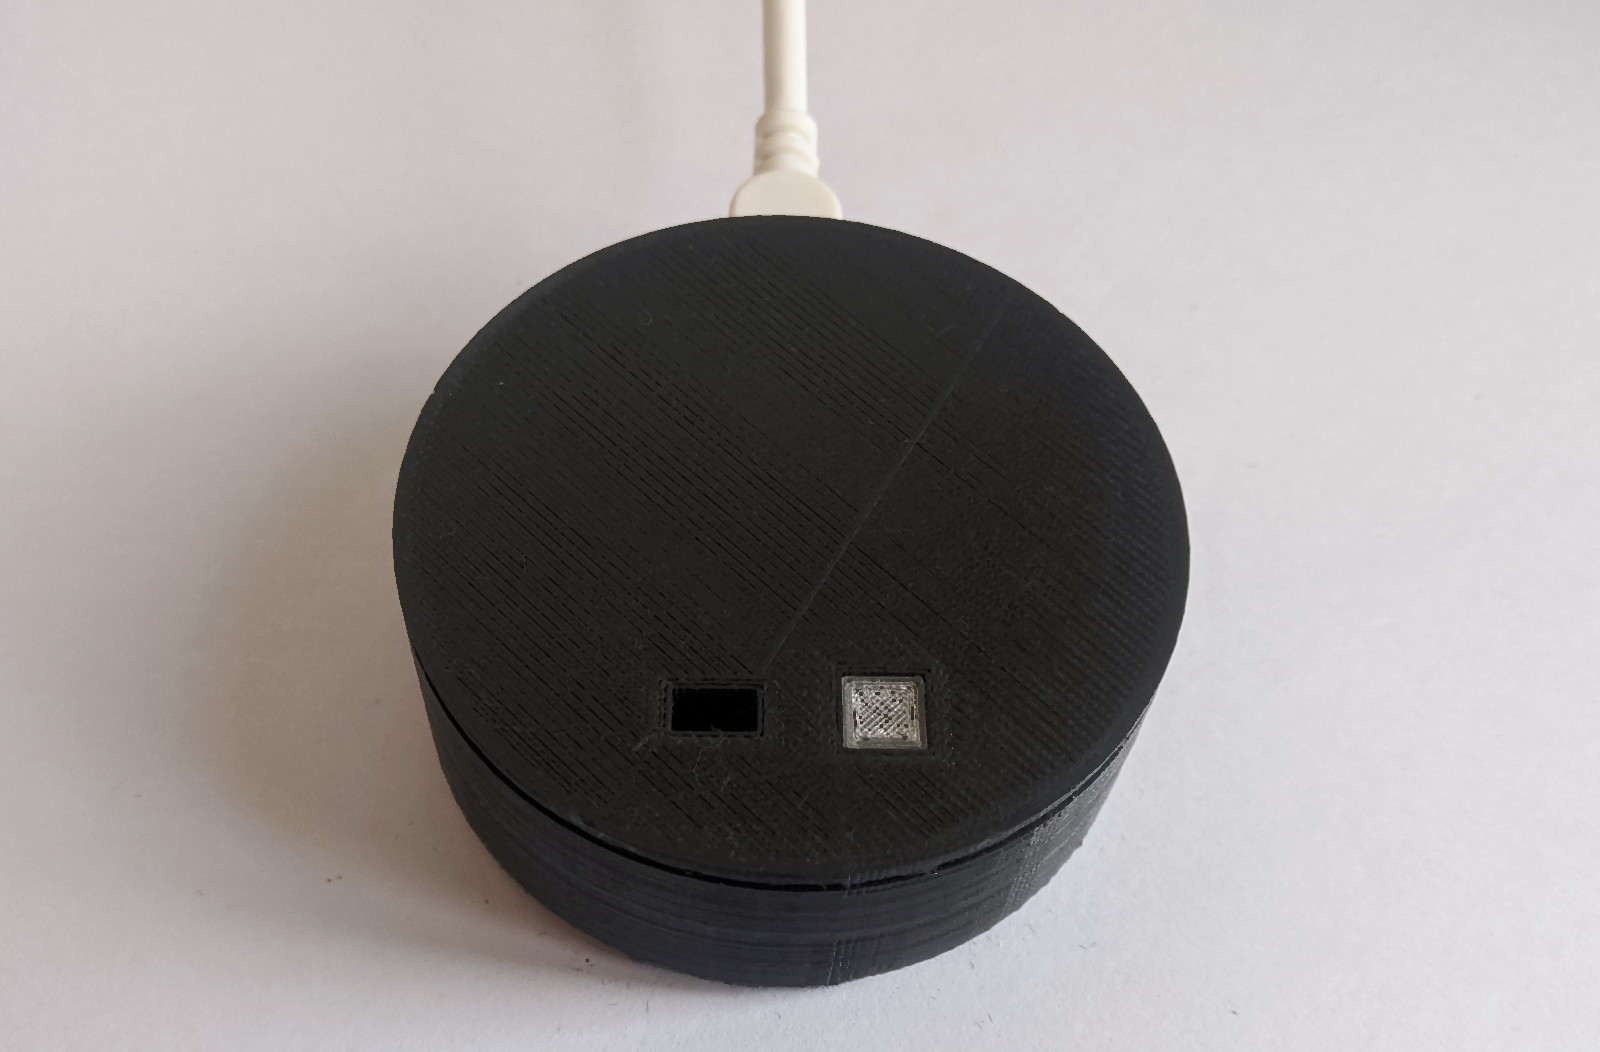
\includegraphics[width=\textwidth]{Dispositivo_files/assembly_15.jpg}
	\caption{Dispositivo OpenLDAT assemblato}
	\label{fig:assembly_15}
\end{figure}

\subsection{Flashing}
Il dispositivo OpenLDAT è inutile senza il suo firmware, per cui va programmato prima di utilizzarlo. Vengono forniti due metodi per caricare il firmware:
\begin{itemize}
	\item \textbf{Script automatico}: assieme al firmware viene fornito uno script che carica sul dispositivo un firmware precompilato e testato. Questa è la soluzione consigliata per chi vuole solo utilizzare OpenLDAT e non sviluppare. Al momento lo script è disponibile per GNU/Linux e Windows
	\item \textbf{Usando Arduino IDE}: il progetto del firmware può essere caricato in Arduino IDE e caricato sul dispositivo da lì. Questa è la soluzione ideale per chi vuole sviluppare versioni modificate del firmware, ma richiede che l'IDE venga configurata opportunamente e introduce alcune complicazioni
\end{itemize}

Le due sezioni successive spiegano passo-passo come eseguire il \textit{flashing} il dispositivo con questi due metodi.

\subsubsection{Flashing con lo script automatico (GNU/Linux)}
All'interno della cartella del firmware è presente una cartella chiamata \texttt{Prebuilt}, all'interno della quale è presente il firmware precompilato e lo script \texttt{flash.sh}.

\paragraph{Passo 1} Installare python e avrdude dal gestore dei pacchetti della propria distribuzione. Supponendo di essere su Ubuntu, questo comando installa i due package necessari per il \textit{flashing}:
\begin{verbatim}
	sudo apt install python3 avrdude
\end{verbatim}

\paragraph{Passo 2} Aprire un terminale all'interno della cartella \texttt{Prebuilt}, collegare il dispositivo da programmare e prendere nota del nome che viene assegnato alla porta seriale del dispositivo. Questo comando permette di elencare le porte seriali attualmente assegnate:
\begin{verbatim}
	ls -l /dev/serial/by-id
\end{verbatim}

Nell'esempio in figura \ref{fig:flashing_01}, al dispositivo viene assegnato il nome \texttt{ttyACM0}.

\paragraph{Passo 3} Eseguire il \textit{flashing} del dispositivo con il seguente comando, sostituendo a \texttt{device} il nome della porta seriale determinato nel passo precedente:
\begin{verbatim}
	sudo ./flash.sh /dev/device
\end{verbatim}

Lo script richiederà alcuni secondi per essere eseguito, durante i quali produce un output dettagliato delle attività. Se la procedura viene completata correttamente, al termine viene visualizzato il messaggio \textit{``Successs! You now have an OpenLDAT device''} come in figura \ref{fig:flashing_02}.\\
Se si verificano degli errori durante la procedura, i dettagli verranno mostrati per consentire di capire il problema.

Attenzione: è raro ma possibile che il nome della porta seriale assegnata al dispositivo cambi durante l'esecuzione dello script facendolo fallire. Se dovesse succedere, si può riprovare con un'altra porta USB o un altro PC, oppure utilizzando Arduino IDE.

\begin{figure}[H]
	\centering
	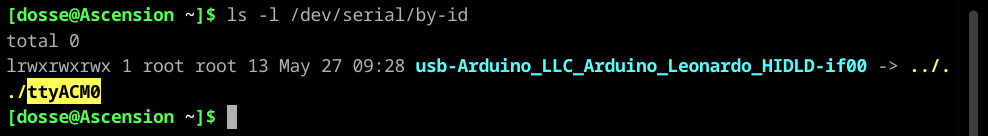
\includegraphics[width=\textwidth]{Dispositivo_files/flashing_01.png}
	\caption{Esempio di elenco dei dispositivi seriali}
	\label{fig:flashing_01}
\end{figure}

\begin{figure}[H]
	\centering
	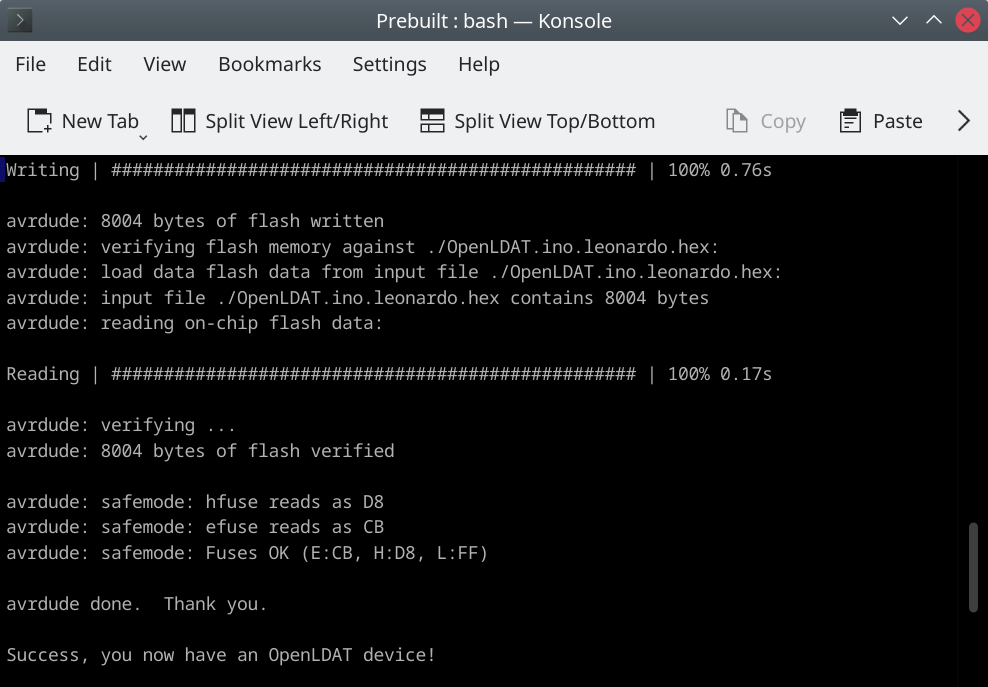
\includegraphics[width=\textwidth]{Dispositivo_files/flashing_02.png}
	\caption{Output dello script automatico}
	\label{fig:flashing_02}
\end{figure}

\subsubsection{Flashing con lo script automatico (Windows)}
All'interno della cartella del firmware è presente una cartella chiamata \texttt{Prebuilt}, all'interno della quale è presente il firmware precompilato e lo script \texttt{flash.bat} per Windows.

\paragraph{Passo 1} Installare Arduino IDE utilizzando l'installatore sul sito web\footnote{\url{https://www.arduino.cc/en/software}}, lasciando i file nel loro percorso di default, e assicurandosi di installare anche i driver di Arduino.

\paragraph{Passo 2} Collegare il dispositivo da programmare, entrare nella cartella \texttt{Prebuilt} e fare doppio click su \texttt{flash.bat} per visualizzare l'elenco di porte COM, come in figura figura \ref{fig:flashing_07}. Prendere nota della porta del dispositivo, nell'esempio è \texttt{COM6}.

\paragraph{Passo 3} Aprire un terminale all'interno della cartella Prebuilt ed eseguire il seguente comando, sostituendo a \texttt{COM6} la porta del dispositivo da programmare determinata nel passo precedente:
\begin{verbatim}
	.\flash.bat COM6
\end{verbatim}

Lo script richiederà alcuni secondi per essere eseguito, durante i quali produce un output dettagliato delle attività. Se la procedura viene completata correttamente, al termine viene visualizzato il messaggio \textit{``Successs! You now have an OpenLDAT device''} come in figura \ref{fig:flashing_08}.\\
Se si verificano degli errori durante la procedura, i dettagli verranno mostrati per consentire di capire il problema.

Attenzione: l'installazione automatica dei driver di Windows Update potrebbe interferire durante la procedura di \textit{flashing}. Se dovesse succedere, rieseguire la procedura dal Passo 2.

\begin{figure}[H]
	\centering
	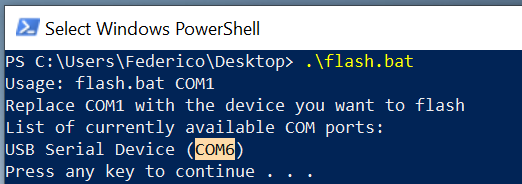
\includegraphics[width=.7\textwidth]{Dispositivo_files/flashing_07.png}
	\caption{Esempio di elenco di porte COM}
	\label{fig:flashing_07}
\end{figure}

\begin{figure}[H]
	\centering
	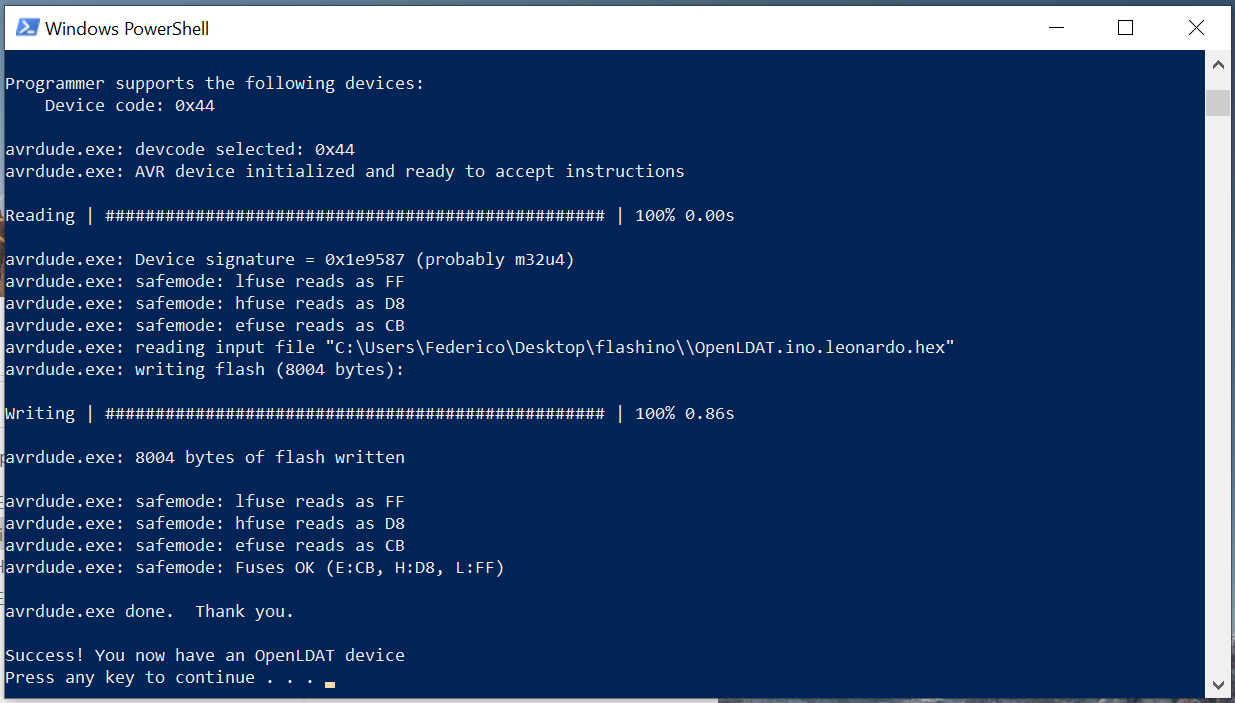
\includegraphics[width=\textwidth]{Dispositivo_files/flashing_08.png}
	\caption{Output dello script automatico}
	\label{fig:flashing_08}
\end{figure}

\subsubsection{Flashing con Arduino IDE}
Il \textit{flashing} con Arduino IDE è consigliato per chi vuole contribuire al progetto con modifiche al firmware.

\paragraph{Passo 1} Installare Arduino IDE. Se si sta utilizzando Windows, assicurarsi di installare anche i driver.

\paragraph{Passo 2} Aggiungere il dispositivo OpenLDAT Model 1 all'elenco delle board AVR riconosciute da Arduino IDE. Per farlo, bisogna modificare il relativo file \texttt{boards.txt}

Su Windows, il file si trova nel seguente percorso:\\
	\texttt{C:\textbackslash Program Files (x86)\textbackslash Arduino\textbackslash hardware\textbackslash arduino\textbackslash avr\textbackslash boards.txt}

Su GNU/Linux, il file si trova tipicamente in uno dei seguenti percorsi (dipende dalla distribuzione utilizzata):\\
	\texttt{/usr/share/arduino/hardware/arduino/avr/boards.txt}\\
	\texttt{/usr/share/arduino/hardware/archlinux-arduino/avr/boards.txt}\\
	\texttt{/usr/share/arduino/hardware/arduino/boards.txt}

Su MacOS, il file si trova nel seguente percorso:\\
	\texttt{\textasciitilde/Library/Arduino/hardware/arduino/avr/boards.txt}

Una volta localizzato il file, aggiungere il seguente listato alla fine del file e salvare.
\lstinputlisting{Dispositivo_files/boards.txt}

\paragraph{Passo 3} Collegare il dispositivo da programmare e avviare Arduino IDE. Se è stato fatto tutto correttamente, dovrebbe essere possibile selezionare il dispositivo dall'elenco di porte seriali (figura \ref{fig:flashing_03}) e dovrebbe essere possibile selezionare come modello il dispositivo OpenLDAT Model 1 (figura \ref{fig:flashing_04}).

\paragraph{Passo 4} Aprire il gestore delle librerie di Arduino IDE e scaricare la libreria HID-Project di NicoHood (figura \ref{fig:flashing_06}). Qualora non fosse disponibile, è inclusa una copia della libreria nel file \texttt{Libraries.zip} nella cartella del firmware, che può essere estratta nella cartella libraries di Arduino.

\paragraph{Passo 5} Caricare il progetto \texttt{OpenLDAT} presente nella cartella del firmware in Arduino IDE e premere il pulsante \textit{Upload} (figura \ref{fig:flashing_05}). A questo punto il dispositivo ha il firmware ed è pronto all'uso.

Attenzione: su alcune distribuzioni GNU/Linux è necessario dare al proprio utente i permessi per accedere alle porte seriali o eseguire Arduino IDE con sudo per poter programmare il dispositivo.

Attenzione: è raro ma possibile che il nome della porta seriale assegnata al dispositivo cambi durante il \textit{flashing} facendolo fallire. Arduino IDE tenterà di rimediare questa cosa, ma se non riesce si può riprovare con un'altra porta USB o un altro PC.

Attenzione: il \textit{flashing} con Arduino IDE introduce il problema della riproducibilità delle build. A seconda della versione del compilatore GCC e delle librerie Arduino, il firmware potrebbe essere eseguito a velocità leggermente diverse da quelle che si aspetta l'applicazione senza che questa abbia modo di saperlo. Sebbene questo non alteri significativamente le misurazioni eseguite dall'applicazione (c'è una differenza dell'1-2\%), è bene esserne a conoscenza.

\begin{figure}[H]
	\centering
	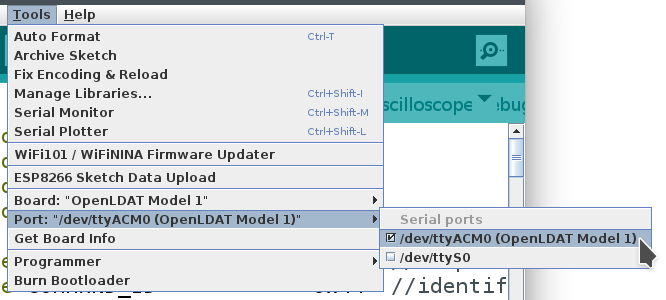
\includegraphics[width=0.8\textwidth]{Dispositivo_files/flashing_03.png}
	\caption{Selezione del dispositivo (potrebbe avere un nome diverso da Arduino Leonardo, dipende dal bootloader caricato in fabbrica)}
	\label{fig:flashing_03}
\end{figure}

\begin{figure}[H]
	\centering
	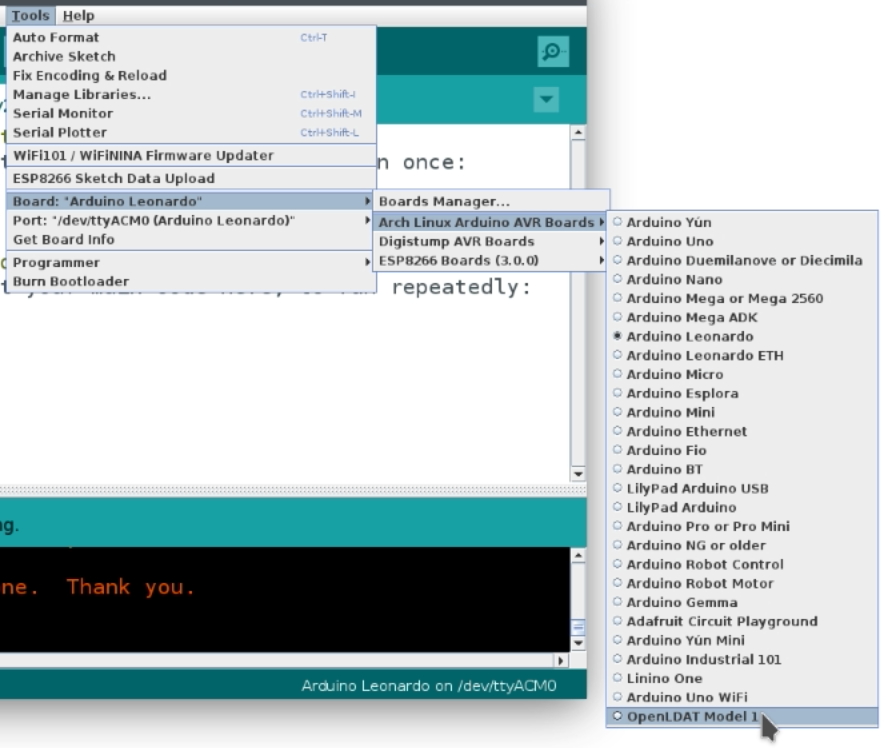
\includegraphics[width=\textwidth]{Dispositivo_files/flashing_04.png}
	\caption{Selezione del modello}
	\label{fig:flashing_04}
\end{figure}

\begin{figure}[H]
	\centering
	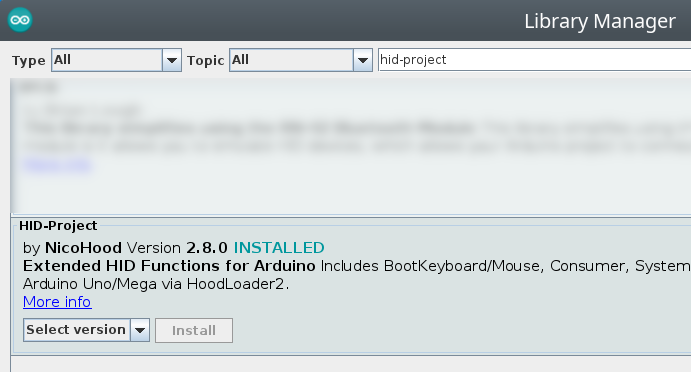
\includegraphics[width=0.8\textwidth]{Dispositivo_files/flashing_06.png}
	\caption{Download della libreria HID-Project}
	\label{fig:flashing_06}
\end{figure}

\begin{figure}[H]
	\centering
	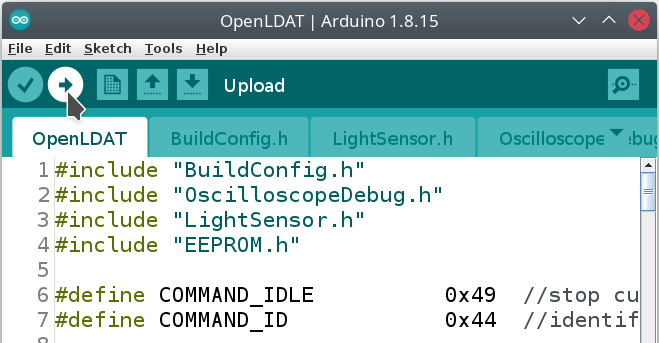
\includegraphics[width=0.8\textwidth]{Dispositivo_files/flashing_05.png}
	\caption{Pronto per il \textit{flashing}}
	\label{fig:flashing_05}
\end{figure}

Questo conclude il capitolo sulla parte fisica del progetto OpenLDAT. Nei capitoli successivi l'attenzione si sposterà principalmente sul software. %La parte spirituale non verrà trattata in questa tesi.

\newpage
\chapter{L'applicazione OpenLDAT}
\label{chap:app}

Questo capitolo si concentra sull'applicazione OpenLDAT per PC, illustrandone i requisiti, le tecnologie utilizzate e i dettagli del funzionamento, con un focus particolare agli algoritmi che analizzano i dati raccolti dal dispositivo.

I requisiti principali per l'applicazione OpenLDAT sono i seguenti:
\begin{itemize}
	\item Implementare dei test che utilizzano il dispositivo OpenLDAT per raccogliere dati e li analizzano per estrarre informazioni
	\item I test implementati devono essere il più possibile rappresentativi dell'utilizzo reale del sistema
	\item Funzionare su più sistemi operativi, almeno GNU/Linux, Windows e MacOS
	\item Essere facile da installare e utilizzare anche per un utente poco esperto
\end{itemize}

Prima di iniziare lo sviluppo sono state prese in considerazione più tecnologie per implementare l'applicazione: inizialmente sono stati fatti degli esperimenti con Electron, che oggi è molto popolare per sviluppare applicazioni desktop multipiattaforma, ma si sono presto presentate difficoltà dovute al fatto che l'engine Chromium al suo interno introduce esso stesso un notevole ritardo di input, per cui i test non sarebbero stati rappresentativi; la scelta finale è quindi ricaduta su Java SE con OpenGL, scelta che consente molta più libertà di implementazione, e di realizzare quindi test più rappresentativi di un utilizzo reale.

L'applicazione è strutturata in quattro parti principali più alcune classi di utilità:
\begin{itemize}
	\item \textbf{Comunicazione con il dispositivo} (package \texttt{com.dosse.openldat.device}): è sostanzialmente un driver per il dispositivo OpenLDAT che ha il compito di rilevare il dispositivo e consentire al resto dell'applicazione di utilizzarlo in modo semplice, senza preoccuparsi dei dettagli di comunicazione
	\item \textbf{Elaborazione di base} (package \texttt{com.dosse.openldat.processing}): fornisce un insieme di strumenti per memorizzare i dati in arrivo dal dispositivo e dei filtri che possono essere applicati su di essi (ad esempio, FFT)
	\item \textbf{I test} (package \texttt{com.dosse.openldat.tests}): questa è la parte principale dell'applicazione e implementa tutti i test che sono stati sviluppati per OpenLDAT, oltre a due backend grafiche per disegnare sullo schermo con e senza OpenGL
	\item \textbf{La GUI} (package \texttt{com.dosse.openldat.ui}): implementa l'interfaccia grafica per l'applicazione che permette di configurare ed eseguire i test e visualizzarne in modo grafico i risultati
\end{itemize}

Oltre a Java SE, per lo sviluppo dell'applicazione sono state utilizzate anche le seguenti librerie:
\begin{itemize}
	\item \textbf{jSerialComm} \footnote{\url{https://github.com/Fazecast/jSerialComm}}: una libreria che consente ad applicazioni Java di interfacciarsi con dispositivi seriali
	\item \textbf{LWJGL} \footnote{\url{https://www.lwjgl.org/}}: una libreria per lo sviluppo di applicazioni OpenGL in Java, utilizzata anche da giochi commerciali come Minecraft
	\item \textbf{JTransforms} \footnote{\url{https://github.com/wendykierp/JTransforms}}: utilizzata per realizzare il filtro FFT
\end{itemize}

Tutti i file relativi all'applicazione e al packaging per le varie piattaforme sono presenti nella cartella \texttt{App} all'interno del repository. Il progetto \texttt{OpenLDAT} al suo interno può essere caricato in NetBeans IDE.

Nelle sezioni successive verranno discussi approfonditamente tutti gli aspetti dell'applicazione.

\section{Comunicazione col dispositivo}
Questa sezione si concentra sul package \texttt{com.dosse.openldat.device}, che implementa tutta la parte di comunicazione con il dispositivo OpenLDAT.

\subsection{DeviceFinder}
La comunicazione col dispositivo avviene tramite l'interfaccia seriale USB esposta dal dispositivo, ma prima di poter comunicare con esso, bisogna trovarlo. Poiché al PC potrebbero essere connessi più dispositivi seriali, l'applicazione distingue i dispositivi OpenLDAT dagli altri grazie all'ID hardware impostato dal firmware come spiegato nel capitolo precedente.
Il processo di rilevazione dei dispositivi è svolto dalla classe \texttt{DeviceFinder}, la quale contiene dei metodi statici per trovare i dispositivi.

\paragraph{Metodi statici:}\begin{itemize}
	\item \texttt{public static SerialPort[] findDevices()}: trova tutti i dispositivi OpenLDAT attualmente connessi e li ritorna come un array di \texttt{SerialPort} (una classe della libreria jSerialComm). Non viene fatto alcun controllo sullo stato del dispositivo stesso, nè del fatto che sia supportato o meno
	\item \texttt{public static Device getDevice()}: un metodo più comodo per ottenere il primo device OpenLDAT connesso al PC supportato dall'applicazione, o \texttt{null} se non ce ne sono. Questo metodo è utile solo per comodità in fase di testing, l'applicazione non lo utilizza. Il metodo ritorna un'istanza di \texttt{Device}, che è la classe che implementa effettivamente la comunicazione con il dispositivo
\end{itemize}

\subsection{Device}
Una volta scelto il dispositivo OpenLDAT da utilizzare, si può istanziare la classe \texttt{Device} passandole la porta seriale scelta. Il costruttore di questa classe esegue tutti i controlli necessari per identificare il dispositivo, verificare che sia supportato e ottiene l'elenco delle \textit{capability}. In seguito, la classe mette a disposizione dei metodi per utilizzare il dispositivo. La classe utilizza un buffer in ricezione di 128kB per evitare di bloccare il dispositivo mentre qualcosa viene processato.

\paragraph{Costruttori:}\begin{itemize}
	\item \texttt{public Device(SerialPort com)}: crea l'istanza di \texttt{Device} utilizzando la porta seriale specificata. Durante l'inizializzazione, viene verificato il modello del dispositivo e viene richiesto l'elenco delle \textit{capability} per inizializzare tutte le variabili interne alla classe. Se il dispositivo non è riconosciuto, non è compatibile, richiede una versione più recente del driver, o l'elenco delle \textit{capability} non è valido, l'inizializzazione fallisce.\\
	Il costruttore può lanciare un'eccezione \texttt{DeviceError} se l'inizializzazione fallisce o una \texttt{IOException} se ci sono problemi di comunicazione durante l'inizializzazione
\end{itemize}

\paragraph{Metodi pubblici:}\begin{itemize}
	\item \texttt{public boolean isOpen()}: ritorna \texttt{true} se la connessione al dispositivo è attualmente aperta
	\item \texttt{public void close()}: chiude la connessione verso il dispositivo in modo sicuro, terminando qualsiasi attività in corso
	\item \texttt{public boolean hasLightSensor()}: ritorna \texttt{true} se il dispositivo è dotato di un sensore di luminosità
	\item \texttt{public boolean isPrototype()}: ritorna \texttt{true} se il dispositivo si dichiara come prototipo. Nella GUI, i prototipi hanno a disposizione un menu di test dedicato
	\item \texttt{public boolean hasOscilloscopeDebug()}: ritorna \texttt{true} se il dispositivo genera pulsazioni sul pin 10 durante l'attività
	\item \texttt{public String getFirmwareVersion()}: ritorna la versione del firmware come una stringa. Per convenzione, le versioni del firmware contengono la data in formato YYYYMMDD seguita opzionalmente da altri caratteri, ad esempio \texttt{20210225-production}
	\item \texttt{public String getModel()}: ritorna il modello completo del dispositivo come dichiarato dal firmware, non dall'ID hardware
	\item \texttt{public int getModelCode()}: ritorna il modello del dispositivo come numero. Attualmente, il dispositivo OpenLDAT Model 1 è l'unico supportato ed ha il codice 1
	\item \texttt{public String getPortName()}: ritorna il nome della porta seriale del dispositivo
	\item \texttt{public int getMinDriverVersion()}: ritorna il codice di versione minimo del driver richiesto dal dispositivo come dichiarato dal firmware. La versione attuale del driver ha codice di versione 1
	\item \texttt{public String getSerialNumber()}: ritorna il numero di serie del dispositivo come stringa, o la stringa \texttt{DIY} se non ce l'ha
	\item \texttt{public boolean isBusy()}: ritorna \texttt{true} se il dispositivo sta eseguendo qualche attività ed è occupato
	\item \texttt{public void endCurrentActivity()}: termina l'attività corrente e attende che il dispositivo torni in stato \textit{idle} per accettare nuovi comandi. Questo metodo è bloccante fino a quando il dispositivo non è in stato \textit{idle}. L'esecuzione richiede circa 100ms. Questo metodo va utilizzato solo per interrompere un'attività (ad esempio alla fine di un test), se si desidera passare da un'attività a un'altra, quella precedente viene interrotta automaticamente dalla nuova
	\item \texttt{public double lightSensorMonitorMode(boolean noBuffer, byte sensitivity, boolean fastADC, LightSensorMonitorCallback callback)}: avvia il campionamento del sensore di luminosità sul dispositivo, senza pulsante.\begin{itemize}
		\item \texttt{boolean noBuffer}: se impostato a \texttt{true}, utilizza la modalità senza buffering (più lenta ma campionamento più regolare), altrimenti utilizza la modalità con buffering
		\item \texttt{byte sensitivity}: imposta il livello di gain del sensore tra 0 (più basso) e 3 (più alto)
		\item \texttt{boolean fastADC}: se impostato a \texttt{true}, campiona il segnale molto più velocemente
		\item \texttt{LightSensorMonitorCallback callback}: il callback da chiamare quando sono disponibili nuovi dati dal dispositivo. Questa classe verrà approfondita successivamente
	\end{itemize}
	Una volta avviato il campionamento il metodo non è bloccante e ritorna il sample rate del segnale che sta acquisendo.\\
	Se il dispositivo non ha un sensore di luminosità viene lanciata un'eccezione \texttt{MissingSensorException}, se si verificano errori di comunicazione, viene lanciata una \texttt{IOException}.\\
	Se il metodo viene chiamato mentre è già in corso un'altra attività, questa viene terminata automaticamente e quella nuova viene eseguita
	\item \texttt{public double getLightSensorMonitorModeSampleRate(boolean noBuffer, boolean fastADC)}: ritorna la frequenza di campionamento che offrirebbe il dispositivo nel campionare il sensore di luminosità senza il pulsante, con le impostazioni richieste.\begin{itemize}
		\item \texttt{boolean noBuffer}: se impostato a \texttt{true}, utilizza la modalità senza buffering (più lenta ma campionamento più regolare), altrimenti utilizza la modalità con buffering
		\item \texttt{boolean fastADC}: se impostato a \texttt{true}, campiona il segnale molto più velocemente
	\end{itemize}
	Vedi anche: tabella \ref{tab:openldat_samplerates} (con \texttt{MONITOR=1}).\\
	Viene lanciata un'eccezione \texttt{MissingSensorException} se il dispositivo non ha un sensore di luminosità
	\item \texttt{public double lightSensorButtonMode(boolean noBuffer, byte sensitivity, boolean fastADC, boolean noClick, boolean autoFire, LightSensorButtonCallback callback)}: avvia il campionamento del sensore di luminosità sul dispositivo, con il pulsante.\begin{itemize}
		\item \texttt{boolean noBuffer}: se impostato a \texttt{true}, utilizza la modalità senza buffering (più lenta ma campionamento più regolare), altrimenti utilizza la modalità con buffering
		\item \texttt{byte sensitivity}: imposta il livello di gain del sensore tra 0 (più basso) e 3 (più alto)
		\item \texttt{boolean fastADC}: se impostato a \texttt{true}, campiona il segnale molto più velocemente
		\item \texttt{boolean noClick}: se impostato a \texttt{true}, i click vengono registrati ma non viene simulato un click del mouse
		\item \texttt{boolean autoFire}: se impostato a \texttt{true}, i click vengono generati automaticamente, altrimenti vengono ricevuti tramite il pulsante esterno
		\item \texttt{LightSensorButtonCallback callback}: il callback da chiamare quando sono disponibili nuovi dati dal dispositivo. Questa classe verrà approfondita successivamente
	\end{itemize}
	Una volta avviato il campionamento il metodo non è bloccante e ritorna il sample rate del segnale che sta acquisendo.\\
	Se il dispositivo non ha un sensore di luminosità viene lanciata un'eccezione \texttt{MissingSensorException}, se si verificano errori di comunicazione, viene lanciata una \texttt{IOException}.\\
	Se il metodo viene chiamato mentre è già in corso un'altra attività, questa viene terminata automaticamente e quella nuova viene eseguita
	\item \texttt{public double getLightSensorButtonModeSampleRate(boolean noBuffer, boolean fastADC)}: ritorna la frequenza di campionamento che offrirebbe il dispositivo nel campionare il sensore di luminosità senza il pulsante, con le impostazioni richieste.\begin{itemize}
		\item \texttt{boolean noBuffer}: se impostato a \texttt{true}, utilizza la modalità senza buffering (più lenta ma campionamento più regolare), altrimenti utilizza la modalità con buffering
		\item \texttt{boolean fastADC}: se impostato a \texttt{true}, campiona il segnale molto più velocemente
	\end{itemize}
	Vedi anche: tabella \ref{tab:openldat_samplerates} (con \texttt{MONITOR=0}).\\
	Viene lanciata un'eccezione \texttt{MissingSensorException} se il dispositivo non ha un sensore di luminosità
\end{itemize}

\subsection{Callback e errori}
I package \texttt{com.dosse.openldat.device.callback} e \texttt{com.dosse.openldat.device.errors} contengono le classi che implementano i callback e gli errori menzionate precedentemente.

\subsubsection{DeviceError}
Questa classe estende \texttt{Exception} ed è usata per definire tutti gli errori che possono verificarsi all'interno di \texttt{Device}.

\paragraph{Costruttori:}\begin{itemize}
	\item \texttt{public DeviceError(int type)}: crea l'eccezione utilizzando uno dei tipi predefiniti nella classe stessa (\texttt{FAILED\_TO\_CONNECT}, \texttt{UNSUPPORTED\_MODEL}, \texttt{NOT\_OPENLDAT\_DEVICE}, \texttt{DEVICE\_ID\_FAILED}, \texttt{FIRMWARE\_BUILT\_WITH\_SERIALPLOT}, \texttt{FIRMWARE\_NEEDS\_NEWER\_DRIVER}, \texttt{FIRMWARE\_UNKNOWN}, \texttt{FIRMWARE\_LIGHTSENSOR\_MISSING\_BUFSIZES})
	\item \texttt{public DeviceError(String message)}: crea l'eccezione utilizzando un messaggio personalizzato
\end{itemize}

\paragraph{Metodi pubblici:}\begin{itemize}
	\item \texttt{public int getType()}: ritorna il tipo di eccezione specificata nel costruttore, oppure \texttt{CUSTOM\_ERROR} se è stata inizializzata con un messaggio personalizzato (ottenibile con \texttt{getMessage()})
\end{itemize}

\subsubsection{MissingSensorException}
Questa classe estende \texttt{Exception} ed è usata per gli errori in cui si cerca di utilizzare un sensore non presente sul dispositivo. Funziona in modo analogo a \texttt{DeviceError}.

\paragraph{Costruttori:}\begin{itemize}
	\item \texttt{public MissingSensorException(int type)}: crea l'eccezione utilizzando uno dei tipi predefiniti nella classe stessa (attualmente solo \texttt{LIGHT\_SENSOR})
	\item \texttt{public MissingSensorException(String message)}: crea l'eccezione utilizzando un messaggio personalizzato
\end{itemize}

\paragraph{Metodi pubblici:}\begin{itemize}
	\item \texttt{public int getType()}: ritorna il tipo di eccezione specificata nel costruttore, oppure \texttt{CUSTOM\_ERROR} se è stata inizializzata con un messaggio personalizzato (ottenibile con \texttt{getMessage()})
\end{itemize}

\subsubsection{LightSensorMonitorCallback}
Questa classe implementa i callback per il metodo \texttt{lightSensorMonitorMode} della classe \texttt{Device}. Non è obbligatorio fare l'override di tutti i metodi per utilizzarla.

\paragraph{Metodi pubblici:}\begin{itemize}
	\item \texttt{public void onDataBufferReceived(int[] data){}}: questo callback viene chiamato quando viene ricevuto un nuovo buffer di dati (ossia \texttt{noBuffer} è impostato a \texttt{false}). L'array \texttt{data} contiene i sample ricevuti dal dispositivo sotto forma di interi tra 0 e 1023. La lunghezza dell'array è sempre costante (32 sample).\\
	Attenzione: questo callback deve terminare il prima possibile per evitare di rallentare la lettura dal dispositivo
	\item \texttt{public void onDataSampleReceived(int data){}}: questo callback viene chiamato quando viene ricevuto un nuovo sample dal dispositivo (ossia \texttt{noBuffer} è impostato a \texttt{true}). Il sample è rappresentato con un intero tra 0 e 1023.\\
	Attenzione: questo callback deve terminare il prima possibile per evitare di rallentare la lettura dal dispositivo
	\item \texttt{public void onError(Exception e)}: questo callback viene chiamato se si verifica un errore, per esempio se il dispositivo viene disconnesso mentre si sta campionando. Se non si fa l'override di questo metodo, il suo comportamento di default è stampare l'eccezione e lo 	extit{stack trace}
\end{itemize}

La scelta di tenere metodi separati per la gestione di un intero buffer e per la gestione dei singoli sample è stata fatta perché spesso è possibile applicare qualche tipo di ottimizzazione per ridurre il carico sulla CPU se si lavora su interi buffer anziché singoli sample.

\subsubsection{LightSensorButtonCallback}
Questa classe implementa i callback per il metodo \texttt{lightSensorButtonMode} della classe \texttt{Device}. Il suo funzionamento è analogo a quello di \texttt{LightSensorMonitorCallback}, ma oltre anziché ricevere solo la luce, si riceve anche lo stato del pulsante. Non è obbligatorio fare l'override di tutti i metodi per utilizzarla.

\paragraph{Metodi pubblici:}\begin{itemize}
	\item \texttt{public void onDataBufferReceived(int[] light, int[] click){}}: questo callback viene chiamato quando viene ricevuto un nuovo buffer di dati (ossia \texttt{noBuffer} è impostato a \texttt{false}). L'array \texttt{light} contiene i sample del sensore di luminosità sotto forma di interi tra 0 e 1023, mentre l'array \texttt{click} contiene i sample del pulsante sotto forma di interi tra 0 e 1. I due array hanno la stessa lunghezza. La lunghezza dei due array è sempre costante (21 sample).\\
	Attenzione: questo callback deve terminare il prima possibile per evitare di rallentare la lettura dal dispositivo
	\item \texttt{public void onDataSampleReceived(int light, int click){}}: questo callback viene chiamato quando viene ricevuto un nuovo sample dal dispositivo (ossia \texttt{noBuffer} è impostato a \texttt{true}). L'intero \texttt{light} contiene il valore di luminosità come intero tra 0 e 1023, mentre l'intero \texttt{click} contiene lo stato del pulsante come intero tra 0 e 1.\\
	Attenzione: questo callback deve terminare il prima possibile per evitare di rallentare la lettura dal dispositivo
	\item \texttt{public void onError(Exception e)}: questo callback viene chiamato se si verifica un errore, per esempio se il dispositivo viene disconnesso mentre si sta campionando. Se non si fa l'override di questo metodo, il suo comportamento di default è stampare l'eccezione e lo 	extit{stack trace}
\end{itemize}

\subsection{Esempio di utilizzo}
Nel seguente listato viene mostrato come è possibile utilizzare le classi appena descritte per collegarsi al dispositivo e stampare i valori del sensore di luminosità e del pulsante sul terminale.
\lstinputlisting[language=Java]{Applicazione_files/DeviceExample.java}

\section{Elaborazione di base}
I dati catturati dal sensore, dopo che sono stati ricevuti, devono essere memorizzati per poter estrarre informazioni utili. Per fare questo, il package \texttt{com.dosse.openldat.processing} fornisce dei buffer e alcuni filtri per rendere più facile l'analisi che in seguito sarà svolta dal codice dei test.

\subsection{Buffer}
L'obiettivo dei buffer in questa applicazione è quello di memorizzare gli ultimi $N$ sample ricevuti, così da poterli analizzare in seguito, senza limiti di tempo.\\
Nel package \texttt{com.dosse.openldat.processing.buffers} vengono forniti due tipi di buffer e l'interfaccia generica per i buffer, che ora saranno discussi in dettaglio.

Nota: poiché tutti i dati ricevuti dal dispositivo sono numeri interi, i buffer sono pensati per memorizzare solo quelli, non fanno uso di generics.

\subsubsection{IBuffer}
L'interfaccia \texttt{IBuffer} definisce i metodi che tutti i buffer devono implementare.

\paragraph{Metodi da implementare:}\begin{itemize}
	\item \texttt{public void add(int val)}: aggiunge un singolo intero al buffer
	\item \texttt{public void add(int[] data)}: aggiunge un array di interi al buffer
	\item \texttt{public int[] getData()}: ritorna il contenuto attuale del buffer in maniera sicura (rispettando l'incapsulamento e in modo \textit{thread-safe})
	\item \texttt{public int[] getDataUnsafe()}: ritorna il contenuto attuale del buffer in maniera insicura (non rispetta l'incapsulamento e non è \textit{thread-safe})
	\item \texttt{public int getSize()}: ritorna la dimensione del buffer, ossia quanti interi può contenere il buffer prima di sovrascrivere dei dati
	\item \texttt{public boolean isFilled()}: ritorna \texttt{true} se il buffer è pieno, ossia se sono già stati aggiunti abbastanza dati per evitare che ci siano celle vuote chiamando \texttt{getData}
\end{itemize}

\subsubsection{CircularBuffer}
Questa classe implementa una variante di un buffer circolare che permette di memorizzare gli ultimi $N$ sample aggiunti al buffer, con operazioni di aggiunta e lettura del buffer molto veloci.\\
Nonostante il nome, non è un buffer circolare in senso stretto, poiché il puntatore di scrittura e di lettura coincidono, ma questo è ciò di cui abbiamo bisogno per realizzare l'applicazione e velocizza notevolmente il codice.\\
Tutte le operazioni di questa classe utilizzano i metodi di copia di memoria del sistema anziché dei cicli, migliorando notevolmente le prestazioni.

La classe è \textit{thread-safe}.

\paragraph{Costruttori:}\begin{itemize}
	\item \texttt{public CircularBuffer(int size)}: inizializza un buffer circolare di dimensione \texttt{size}
\end{itemize}

\paragraph{Metodi pubblici:}\begin{itemize}
	\item \texttt{public void add(int val)}: aggiunge un singolo intero al buffer. Se è pieno, viene sovrascritto il valore più vecchio
	\item \texttt{public void add(int[] data)}: aggiunge un array di interi al buffer. Se è pieno, vengono sovrascritti i valori più vecchi
	\item \texttt{public int[] getData()}: ritorna il contenuto attuale del buffer in maniera sicura (rispettando l'incapsulamento e in modo \textit{thread-safe})
	\item \texttt{public int[] getDataUnsafe()}: non supportato su un buffer circolare, esegue semplicemente \texttt{getData}
	\item \texttt{public int[] getInternalBuffer()}: ritorna l'array usato internamente per memorizzare i dati. I dati potrebbero non essere in ordine
	\item \texttt{public int getSize()}: ritorna la dimensione del buffer, ossia quanti interi può contenere il buffer prima di sovrascrivere dei dati
	\item \texttt{public boolean isFilled()}: ritorna \texttt{true} se il buffer è pieno, ossia se sono già stati aggiunti abbastanza dati per evitare che ci siano celle vuote chiamando \texttt{getData}
\end{itemize}

\subsubsection{ArrayBuffer}
Questa è implementa un buffer costante (non è possibile aggiungere nulla). Si tratta di una classe di utilità, utilizzata quando serve avere un array sotto forma di buffer.

La classe è \textit{thread-safe}.

\paragraph{Costruttori:}\begin{itemize}
	\item \texttt{public ArrayBuffer(int[] data)}: inizializza il buffer con l'array di dati fornito. Nota: i dati non vengono copiati, ma solo il riferimento, per cui è possibile alterare il contenuto di questo buffer esternamente. Questo è voluto ed è utilizzato nella GUI
\end{itemize}

\paragraph{Metodi pubblici:}\begin{itemize}
	\item \texttt{public void add(int val)}: non supportato, lancia una \texttt{UnsupportedOperationException}
	\item \texttt{public void add(int[] data)}: non supportato, lancia una \texttt{UnsupportedOperationException}
	\item \texttt{public int[] getData()}: ritorna una copia dell'array \texttt{data} con cui è stato inizializzato il buffer
	\item \texttt{public int[] getDataUnsafe()}: ritorna l'array \texttt{data} con cui è stato inizializzato il buffer (riferimento)
	\item \texttt{public int getSize()}: ritorna la dimensione del buffer, ossia la dimensione dell'array \texttt{data} con cui è stato inizializzato
	\item \texttt{public boolean isFilled()}: ritorna sempre \texttt{true}
\end{itemize}

\subsection{Filtri}
Il package \texttt{com.dosse.openldat.processing.filters} contiene alcuni filtri che sono usati per semplificare l'analisi dei dati raccolti. A tutti gli effetti, un filtro non è altro che un tipo speciale di buffer, che però esegue un qualche tipo di elaborazione sui dati che gli vengono inseriti.

\subsubsection{FFTFilter}
Questa classe implementa un filtro che permette di inserire dati nel dominio del tempo (sample) e ottenere una rappresentazione degli stessi dati nel dominio di frequenza utilizzando una FFT (\textit{Fast Fourier Transform}). La trasformazione viene eseguita dalla libreria jTransforms, ma prima viene applicata ai dati una funzione di windowing di Blackman-Harris, per generare dati più puliti. Per velocizzare l'esecuzione, l'FFT non viene eseguita ad ogni sample aggiunto, ma solo nel momento in cui vengono richiesti i dati.

La classe è \textit{thread-safe}.

\paragraph{Costruttori:}\begin{itemize}
	\item \texttt{public FFTFilter(int size)}: inizializza il filtro su un buffer circolare di dimensione \texttt{size}, che deve essere una potenza di 2 (requisito dell'FFT)
\end{itemize}

\paragraph{Metodi pubblici:} \begin{itemize}
	\item \texttt{public void add(int val)}: aggiunge un singolo intero al buffer. Se è pieno, viene sovrascritto il valore più vecchio
	\item \texttt{public void add(int[] data)}: aggiunge un array di interi al buffer. Se è pieno, vengono sovrascritti i valori più vecchi
	\item \texttt{public int[] getData()}: ritorna il contenuto attuale del buffer, ma nel dominio della frequenza. Ogni valore nell'array ritornato è un bin dell'FFT e il suo valore indica la potenza del segnale in quel bin. Per conoscere la frequenza a cui corrisponde l'\textit{i}-esimo bin, è sufficiente usare la seguente formula: ${\frac{i}{size}*(\frac{sampleRate}{2})}$
	\item \texttt{public int[] getDataUnsafe()}: non supportato su un buffer circolare, esegue semplicemente \texttt{getData}
	\item \texttt{public int[] getOriginalData()}: ritorna i dati inseriti nel buffer, nel dominio temporale
	\item \texttt{public int[] getInternalBuffer()}: ritorna l'array usato internamente per memorizzare i dati nel dominio temporale. I dati potrebbero non essere in ordine
	\item \texttt{public int getSize()}: ritorna la dimensione del buffer, ossia quanti interi può contenere il buffer prima di sovrascrivere dei dati
	\item \texttt{public boolean isFilled()}: ritorna \texttt{true} se il buffer è pieno, ossia se sono già stati aggiunti abbastanza dati per evitare che ci siano celle nel buffer
\end{itemize}

\subsubsection{RunningAverageSmoothingFilter}
Questa classe implementa un filtro che ``smussa'' i dati utilizzando una sorta di media mobile.

Il filtro funziona in questo modo: internamente viene mantenuto il valore di output corrente che chiamiamo $currentValue$, inizializzato a 0; ogni volta che viene aggiunto un nuovo sample $new$, si aggiorna in questo modo: ${currentValue=smoothing*currentValue+(1-smoothing)*new}$, dove $smoothing$ è un valore tra 0 e 1 e indica la resistenza che il filtro oppone a cambiare il valore (0 è istantaneo, 1 non cambia mai). Valori tipici per $smoothing$ sono molto vicini a 1.

La classe è \textit{thread-safe}.

\paragraph{Costruttori:} \begin{itemize}
	\item \texttt{public RunningAverageSmoothingFilter(int size, double smoothing)}: inizializza il filtro su un buffer circolare di dimensione \texttt{size} e con il valore di \texttt{smoothing}
\end{itemize}

\paragraph{Metodi pubblici:} \begin{itemize}
	\item \texttt{public void add(int val)}: aggiunge un singolo intero al buffer. Se è pieno, viene sovrascritto il valore più vecchio. Quando viene aggiunto il primo sample, il valore di $currentValue$ viene inizializzato con quel valore
	\item \texttt{public void add(int[] data)}: aggiunge un array di interi al buffer. Se è pieno, vengono sovrascritti i valori più vecchi. Quando viene aggiunto il primo sample, il valore di $currentValue$ viene inizializzato con quel valore
	\item \texttt{public int[] getData()}: ritorna il contenuto attuale del buffer in maniera sicura (rispettando l'incapsulamento e in modo \textit{thread-safe})
	\item \texttt{public int[] getDataUnsafe()}: non supportato su un buffer circolare, esegue semplicemente \texttt{getData}
	\item \texttt{public int[] getInternalBuffer()}: ritorna l'array usato internamente per memorizzare i dati. I dati potrebbero non essere in ordine
	\item \texttt{public int getSize()}: ritorna la dimensione del buffer, ossia quanti interi può contenere il buffer prima di sovrascrivere dei dati
	\item \texttt{public boolean isFilled()}: ritorna \texttt{true} se il buffer è pieno, ossia se sono già stati aggiunti abbastanza dati per evitare che ci siano celle vuote chiamando \texttt{getData}
\end{itemize}

\subsubsection{PeakHoldFilter}
Questa classe implementa un filtro che mantiene i picchi del segnale dato in ingresso. Ogni sample in output generato dal filtro contiene il valore massimo di una finestra di sample inseriti precedentemente. Questa classe è particolarmente utile per elaborare segnali misurati su display con retroilluminazione PWM.

La classe è \textit{thread-safe}.

\paragraph{Costruttori:}\begin{itemize}
	\item \texttt{public PeakHoldFilter(int size, int peakWindowSize)}: inizializza il filtro con una dimensione del buffer di \texttt{size} e una dimensione della finestra in cui ricercare il massimo di \texttt{peakWindowSize}
\end{itemize}

\paragraph{Metodi pubblici:}\begin{itemize}
	\item \texttt{public void add(int val)}: aggiunge un singolo intero al buffer. Se è pieno, viene sovrascritto il valore più vecchio
	\item \texttt{public void add(int[] data)}: aggiunge un array di interi al buffer. Se è pieno, vengono sovrascritti i valori più vecchi
	\item \texttt{public int[] getData()}: ritorna il contenuto attuale del buffer in maniera sicura (rispettando l'incapsulamento e in modo \textit{thread-safe})
	\item \texttt{public int[] getDataUnsafe()}: non supportato su un buffer circolare, esegue semplicemente \texttt{getData}
	\item \texttt{public int[] getInternalBuffer()}: ritorna l'array usato internamente per memorizzare i dati. I dati potrebbero non essere in ordine
	\item \texttt{public int getSize()}: ritorna la dimensione del buffer, ossia quanti interi può contenere il buffer prima di sovrascrivere dei dati
	\item \texttt{public boolean isFilled()}: ritorna \texttt{true} se il buffer è pieno, ossia se sono già stati aggiunti abbastanza dati per evitare che ci siano celle vuote chiamando \texttt{getData}
\end{itemize}

\paragraph{Metodi statici:}\begin{itemize}
	\item \texttt{public static int findBestWindowSize(int[] noisyData, int min, int max, int stepSize, int noiseThreshold)}: determina il valore minimo di \texttt{peakWindowSize} da utilizzare per far si che applicando il filtro sull'array \texttt{noisyData}, la differenza tra il valore minimo e massimo dopo il filtraggio sia inferiore a \texttt{noiseThreshold}. \texttt{min} e \texttt{max} permettono di restringere l'intervallo di ricerca del valore di \texttt{peakWindowSize} in quell'intervallo, a passi di \texttt{stepSize}. Ritorna -1 se i dati in input non sono validi
\end{itemize}

\subsection{Esempio di utilizzo}
Il seguente listato mostra un esempio di come è possibile acquisire un segnale dal dispositivo e filtrarlo. I grafici nelle figure \ref{fig:filters_example_original}, \ref{fig:filters_example_smooth} e \ref{fig:filters_example_peakHold} mostrano l'output dei filtri. Il segnale catturato è un LED con una PWM di circa 120Hz con piccoli movimenti del sensore per mostrare meglio il comportamento dei filtri.
\lstinputlisting[language=Java]{Applicazione_files/FiltersExample.java}
\begin{figure}[H]
	\centering
	\begin{tikzpicture}
		\begin{axis}[name=Segnale, xmin=0,xmax=8192,ymin=0,ymax=1023,width=.7\textwidth,xlabel=Sample,ylabel=Valore]
			\addplot[black] file{Applicazione_files/filters_example_original.txt};
		\end{axis}
	\end{tikzpicture}
	\begin{tikzpicture}
		\begin{axis}[name=Spettro, xmin=0,xmax=4000,ymin=0,ymax=150000,width=.7\textwidth,xlabel=Frequenza (Hz),ylabel=Potenza]
			\addplot[black] file{Applicazione_files/filters_example_fft.txt};
		\end{axis}
	\end{tikzpicture}
	\caption{Segnale originale e relativo spettro in frequenza. I picchi sono causati dalla frequenza della PWM}
	\label{fig:filters_example_original}
\end{figure}
\begin{figure}[H]
	\centering
	\begin{tikzpicture}
		\begin{axis}[name=Segnale, xmin=0,xmax=8192,ymin=0,ymax=1023,width=.7\textwidth,xlabel=Sample,ylabel=Valore]
			\addplot[gray] file{Applicazione_files/filters_example_original.txt};
			\addplot[red] file{Applicazione_files/filters_example_smooth.txt};
		\end{axis}
	\end{tikzpicture}
	\caption{Segnale originale (grigio), \texttt{RunningAverageSmoothingFilter} (rosso)}
	\label{fig:filters_example_smooth}
\end{figure}
\begin{figure}[H]
	\centering
	\begin{tikzpicture}
		\begin{axis}[name=Segnale, xmin=0,xmax=8192,ymin=0,ymax=1023,width=.7\textwidth,xlabel=Sample,ylabel=Valore]
			\addplot[gray] file{Applicazione_files/filters_example_original.txt};
			\addplot[red] file{Applicazione_files/filters_example_peakHold.txt};
		\end{axis}
	\end{tikzpicture}
	\caption{Segnale originale (grigio), \texttt{PeakHoldFilter} (rosso)}
	\label{fig:filters_example_peakHold}
\end{figure}

\section{Funzionamento dei test}
Questa sezione è dedicata al funzionamento e all'implementazione dei test presenti nell'applicazione. Per test si intende una procedura di misurazione che utilizza il sensore e il display, non si tratta di unit test. Tutto il codice discusso in questa sezione è parte del package \texttt{com.dosse.openldat.tests}.

In generale, un test utilizza una backend grafica per visualizzare qualcosa sul display mentre cattura i dati dal dispositivo, dopodiché analizza i dati raccolti per estrarre informazioni di interesse.

La principale difficoltà che l'analisi deve saper affrontare è la presenza di rumore sul segnale, e in particolar modo la presenza di retroilluminazione PWM. Il problema è gestito diversamente in ogni test, a seconda dell'informazione che si desidera estrarre, ma in generale si assume che in presenza di retroilluminazione PWM, il segnale di interesse è moltiplicato per un altro segnale di frequenza più alta (come se fosse una modulazione AM) e potenzialmente potrebbe avere anche un offset DC variabile.\\
I grafici in figura \ref{fig:pwm_example} mostrano come potrebbe presentarsi un segnale catturato dal sensore in presenza di PWM rispetto al segnale reale. Display diversi tipicamente hanno forme molto diverse per questo segnale.
\begin{figure}[H]
	\centering
	\begin{tikzpicture}
		\begin{axis}[name=Segnale, xmin=0,xmax=0.2,ymin=0,ymax=1023,width=.45\textwidth,xlabel=Tempo (s),ylabel=Valore,xticklabel style={/pgf/number format/fixed}]
			\addplot[black] file{Applicazione_files/pwm_example_desired.txt};
		\end{axis}
	\end{tikzpicture}
	\begin{tikzpicture}
		\begin{axis}[name=Segnale, xmin=0,xmax=0.2,ymin=0,ymax=1023,width=.45\textwidth,xlabel=Tempo (s),ylabel=Valore,xticklabel style={/pgf/number format/fixed}]
			\addplot[black] file{Applicazione_files/pwm_example_captured.txt};
		\end{axis}
	\end{tikzpicture}
	\caption{Segnale reale (sinistra) e possibile segnale catturato in presenza di retroilluminazione PWM (destra). (Simulato, non è una cattura reale)}
	\label{fig:pwm_example}
\end{figure}

In generale, si può dire che in presenza di retroilluminazione PWM, il segnale originale è ricostruibile osservando i picchi alti del segnale catturato, ma è importante ricordare che la presenza di questo tipo di disturbo impedisce di ricostruire accuratamente il segnale originale, soprattutto se ha componenti ad alta frequenza, e che ci sono momenti in cui la retroilluminazione del display è completamente spenta. Per questo motivo, la presenza di PWM influisce negativamente sull'accuratezza di tutti i test.\\
Indipendentemente dal tipo di retroilluminazione, comunque, è sempre bene impostare la luminosità del display al massimo e disattivare qualsiasi tipo di miglioramento dell'immagine prima di eseguire qualsiasi test, così da avere risultati più veritieri. Se la retroilluminazione varia di intensità durante i test, questi potrebbero produrre risultati non validi.

\subsection{Backend grafiche}
Il package \texttt{com.dosse.openldat.tests.testscreen} mette a disposizione due backend grafiche con cui i test possono disegnare sul display: una che utilizza OpenGL (\texttt{TestScreenGL}) e una che utilizza Swing (\texttt{TestScreenSwing}). La backend OpenGL ha più funzionalità ed è più rappresentativa del comportamento di un'applicazione grafica come un videogioco, mentre la backend Swing è più basilare ed è usata come fallback su sistemi che non supportano OpenGL, ma è più rappresentativa del comportamento di un'interfaccia grafica che di un gioco. La GUI comunque permette di scegliere tra le due backend, se lo si desidera.

L'immagine in figura \ref{fig:testscreen_example} mostra un esempio di output di una backend grafica.

\begin{figure}[h]
	\centering
	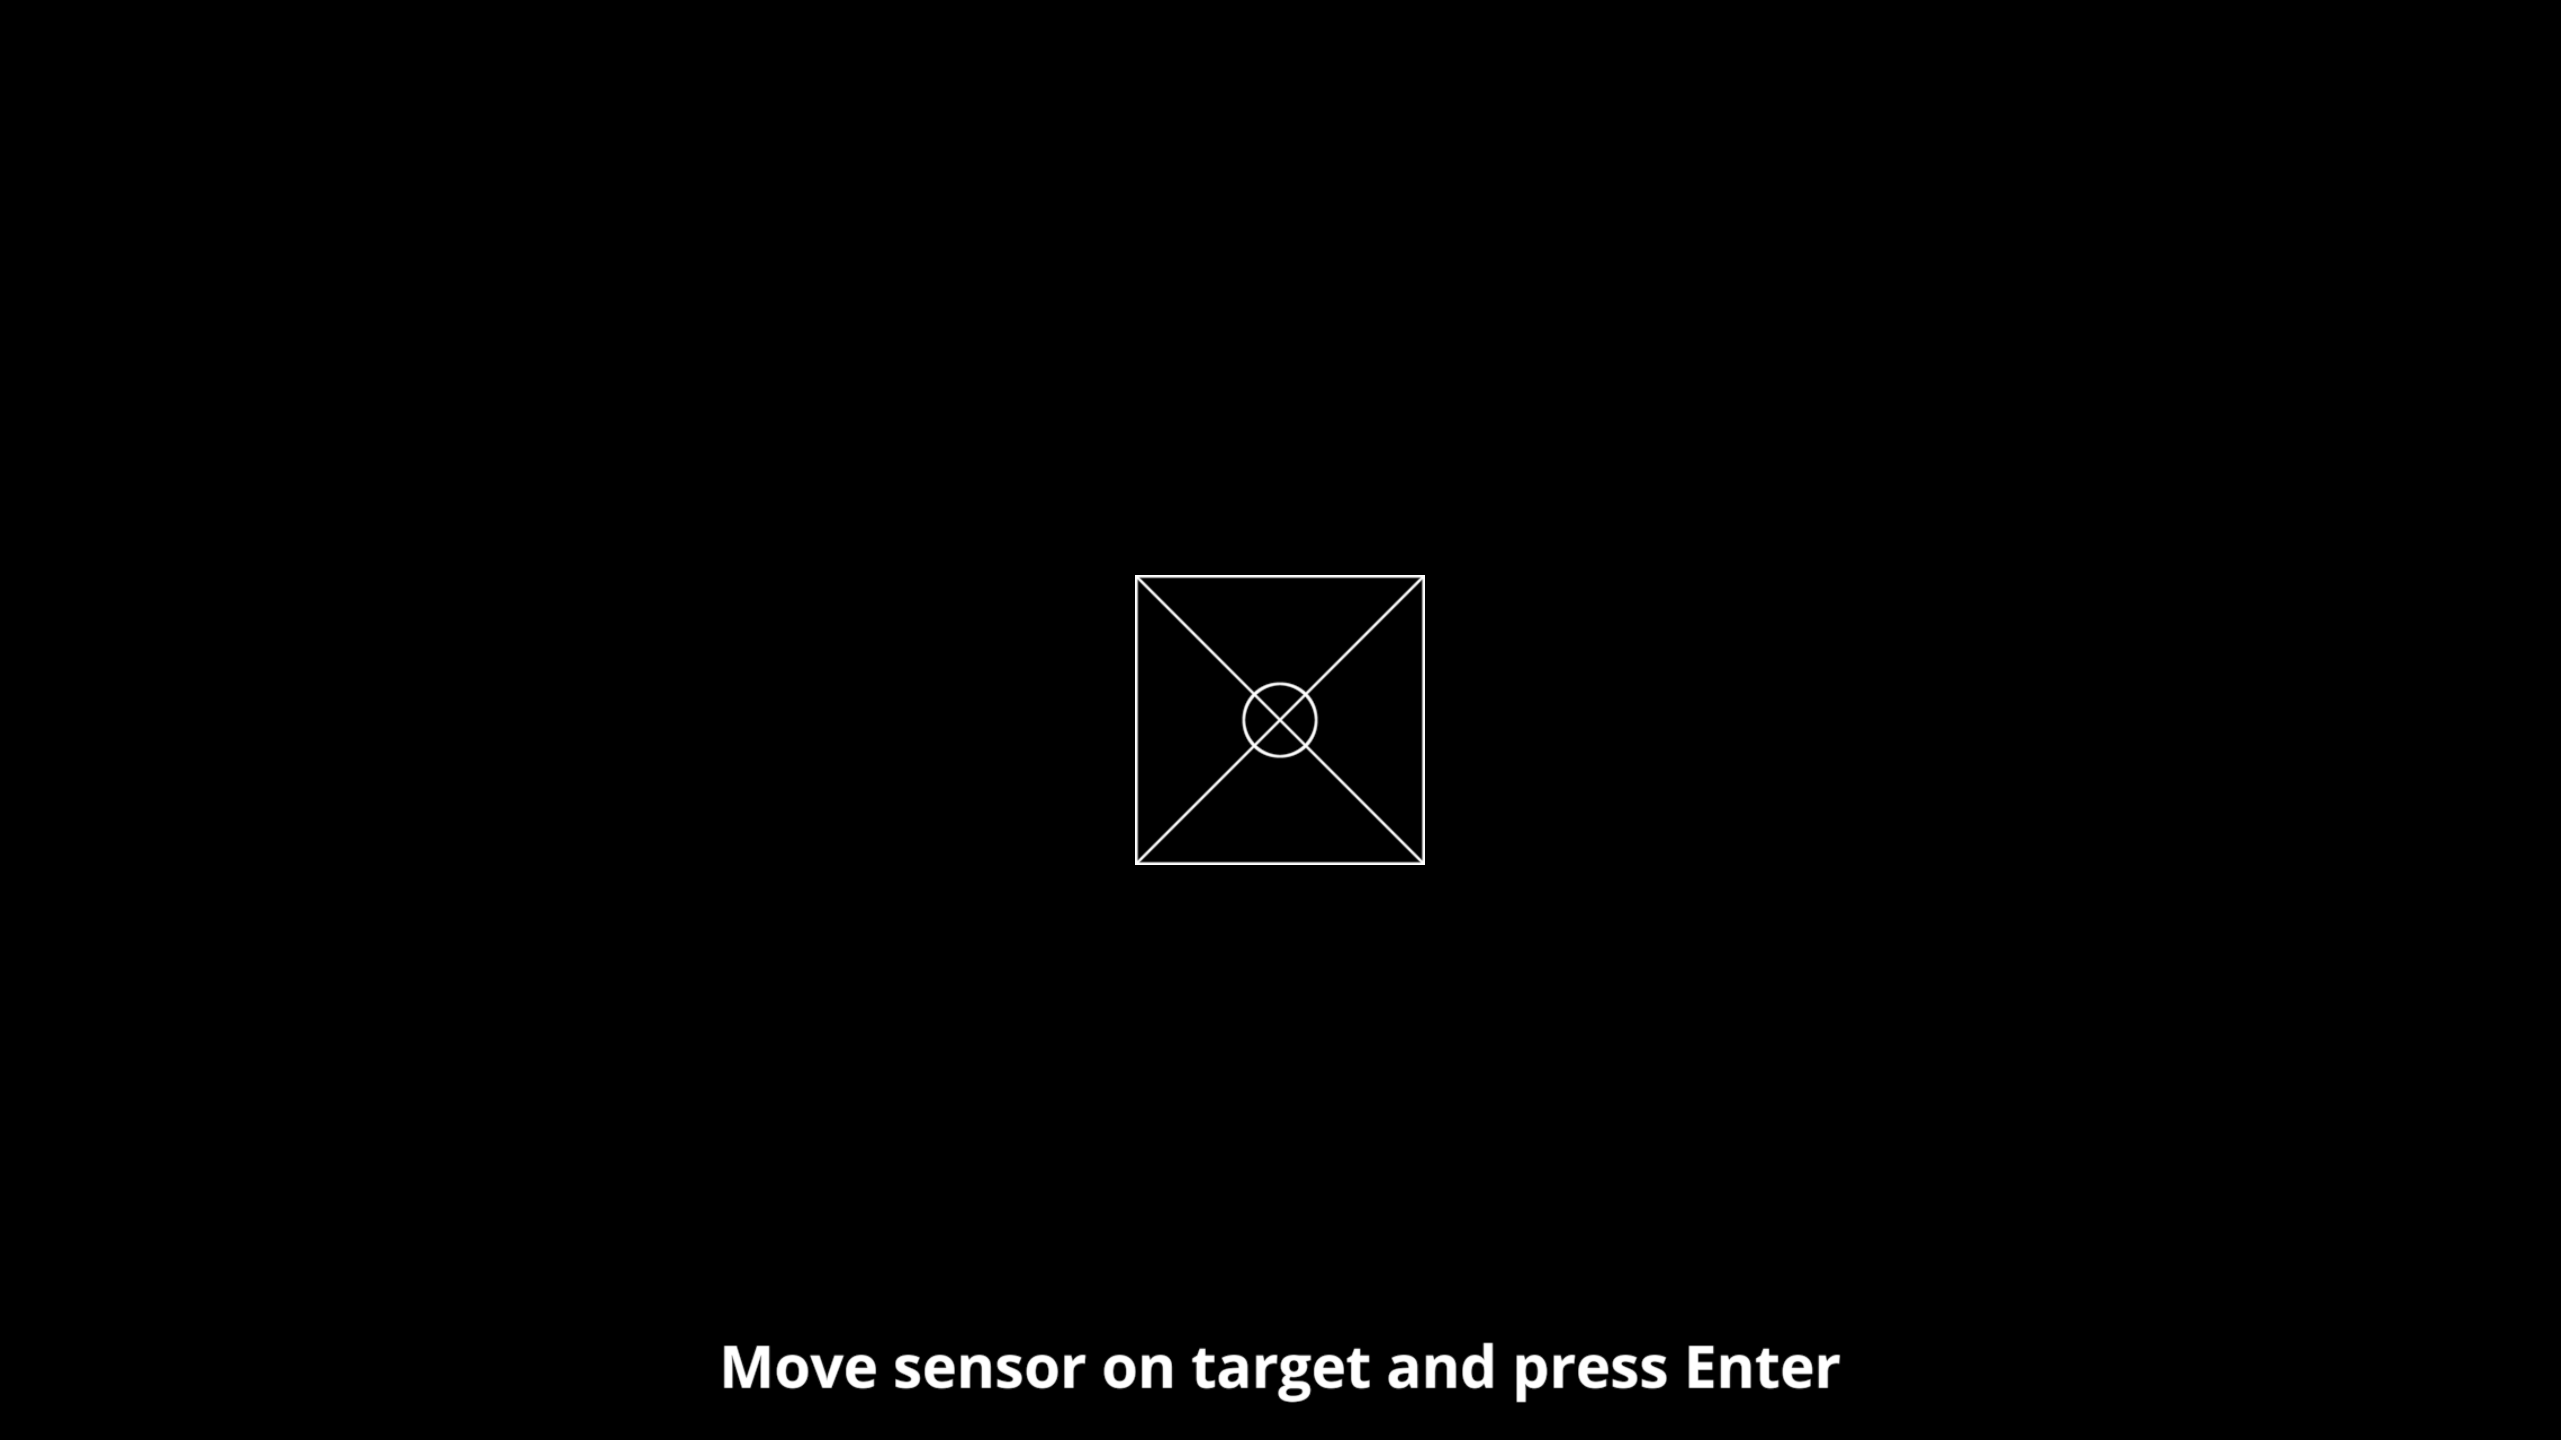
\includegraphics[width=\textwidth]{Applicazione_files/testscreen_example.png}
	\caption{Esempio di output di una schermata di test}
	\label{fig:testscreen_example}
\end{figure}

Entrambe le backend implementano un'interfaccia generica \texttt{ITestScreen}, che definisce le funzionalità minime che un backend deve avere e permette ai test di cambiare backend senza modifiche al codice. L'interfaccia definisce i seguenti metodi pubblici:
\begin{itemize}
	\item \texttt{public int getScreenW()}: ritorna la larghezza dello schermo in pixel
	\item \texttt{public int getScreenH()}: ritorna l'altezza dello schermo in pixel
	\item \texttt{public int getRefreshRate()}: ritorna il \textit{refresh rate} dello schermo in Hz
	\item \texttt{public boolean setColor(float r, float g, float b)}: imposta il colore dello sfondo con tre valori RGB tra 0 e 1. Ritorna \texttt{true} se il colore nuovo è diverso da quello corrente, altrimenti \texttt{false}
	\item \texttt{public void setTarget(float x, float y, float size, boolean black)}: mostra il target e la scritta \textit{``Move sensor on target and press Enter''} alle coordinate specificate. Le coordinate \texttt{x},\texttt{y} si riferiscono al centro del target e vanno tra 0 e 1, dove 0,0 è l'angolo in alto a sinistra e 1,1 è l'angolo in basso a destra. Impostando \texttt{black} a true, il target e il testo saranno di colore nero, altrimenti saranno bianchi. La dimensione del target è definita come ${size*min(W,H)}$. Un valore tipico per \texttt{size} è 0.15. Il target è sempre quadrato
	\item \texttt{public void setTargetAbsolute(float x, float y, float size, boolean black)}: analogo a \texttt{setTarget} ma le coordinate sono assolute anziché nel range 0-1
	\item \texttt{public void hideTarget()}: nasconde il target e la scritta precedentemente attivati con \texttt{setTarget} o \texttt{setTargetAbsolute}
	\item \texttt{public void setFlashOnClick(boolean flashOnClick)}: se impostato a \texttt{true}, quando l'applicazione riceve un click genera un flash bianco di 100ms
	\item \texttt{public boolean getFlashOnClick()}: ritorna \texttt{true} se è attualmente attivo il flash in risposta al click (default: disattivato)
	\item \texttt{public void flashColor(float r, float g, float b, double ms)}: genera un flash del colore specificato dai tre valori RGB tra 0 e 1 e della durata specificata
	\item \texttt{public void setFlicker(boolean bkFlicker)}: se impostato a \texttt{true}, il colore dello sfondo si alterna ad ogni fotogramma tra il colore impostato con \texttt{setColor} e il nero
	\item \texttt{public boolean isFlickering()}: ritorna \texttt{true} se è attualmente attivato il \textit{flickering} (default: disattivato)
	\item \texttt{public void setFakeLoad(long cpuMs, long gpuMs)}: attiva la simulazione di un falso carico sulla CPU e sulla GPU (in millisecondi per frame). Non supportato dalla backend Swing
	\item \texttt{public long getFakeCPULoad()}: ritorna il falso carico attualmente simulato sulla CPU (default: 0)
	\item \texttt{public long getFakeGPULoad()}: ritorna il falso carico attualmente simulato sulla GPU (default: 0)
	\item \texttt{public void close()}: chuiude la schermata di test
	\item \texttt{public void onEnterPressed()}: callback che viene chiamato quando viene premuto il tasto Invio. I test fanno l'override di questo metodo per aggiungere il proprio codice di risposta all'evento. Se non viene fatto l'override, l'evento viene ignorato
	\item \texttt{public void onCancel()}: callback che viene chiamato se viene premuto il tasto \textit{Esc} per annullare il test. I test fanno l'override di questo metodo per aggiungere il proprio codice di risposta all'evento. Se non viene fatto l'override, l'evento viene ignorato
	\item \texttt{public void onError(Exception e)}: callback che viene chiamato se si verificano errori irreversibili, per esempio in seguito a un crash del driver video. I test fanno l'override di questo metodo per aggiungere il proprio codice di risposta all'evento. Se non viene fatto l'override, il comportamento di default è stampare l'eccezione con il relativo 	extit{stack trace} e terminare l'applicazione
\end{itemize}

Le due backend hanno due costruttori leggermente diversi:
\begin{itemize}
	\item \texttt{public TestScreenGL(int vsyncMode)}: inizializza la backend OpenGL 2.0 sullo schermo principale. È possibile specificare una modalità per il \textit{VSync} tra le seguenti costanti definite nella classe stessa:
	\begin{itemize}
		\item \texttt{VSYNC\_OFF}: disabilita il \textit{VSync}, consentendo le massime prestazioni e il minor ritardo possibile
		\item \texttt{VSYNC\_ON}: attiva il \textit{VSync} classico con \textit{double-buffering}
		\item \texttt{VSYNC\_ON\_ALT}: utilizza il \textit{VSync} fornito dal \textit{compositor} del desktop, consentendo all'applicazione di funzionare come se il \textit{VSync} fosse disattivato (quindi a \textit{framerate} illimitato) ma evitando comunque il \textit{tearing}. Non è supportato da tutte le combinazioni hardware e software
	\end{itemize}
	\item \texttt{public TestScreenSwing()}: inizializza la backend Swing sullo schermo principale. Non ci sono impostazioni per questa backend; il \textit{VSync} (se presente) è fornito dal sistema e non è sotto il controllo dell'applicazione
\end{itemize}

Una volta inizializzata, la backend grafica continua l'esecuzione su un thread parallelo, lasciando al thread principale il compito di coordinare il test interagendo con la backend e con il driver del dispositivo.

Prima di proseguire, è necessario puntualizzare alcune caratteristiche delle backend grafiche:\begin{itemize}
	\item Entrambe le backend vengono eseguite in fullscreen \textit{borderless}, non in fullscreen esclusivo. Su GNU/Linux, viene disattivato il \textit{compositor} mentre il test è in esecuzione per evitare che questo penalizzi le performance
	\item La backend OpenGL utilizza lo stesso formato dei pixel e la stessa risoluzione del desktop, tuttavia, a causa di un bug nella libreria LWJGL 3.2.3, l'applicazione potrebbe non dichiarare il supporto HDR/WCG su Windows e quindi mostrare colori errati su display HDR. Questo problema è noto agli sviluppatori di LWJGL e sarà corretto nella release 3.3.0
	\item La backend Swing, poiché utilizza un toolkit grafico pensato per creare interfacce grafiche e non videogiochi, non ha modo di sincronizzarsi con il display, per cui funzioni come \texttt{setFlicker} potrebbero generare un \textit{microstuttering} che non sarebbe normalmente presente in altre applicazioni grafiche
\end{itemize}

\subsection{Interfaccia standard dei test}
I test implementano tutti un'interfaccia comune, \texttt{ITest}, che definisce alcuni metodi che tutti i test devono implementare:
\begin{itemize}
	\item \texttt{public void begin()}: inizia l'esecuzione del codice del test. A seconda del test, questo può significare l'inizio effettivo del test o semplicemente un'operazione come chiedere all'utente di posizionare il sensore
	\item \texttt{public void cancel()}: richiede al test di terminare il prima possibile. A seconda di come è implementato il test, questo potrebbe terminare immediatamente o richiedere del tempo
	\item \texttt{public void onDone(Map results)}: callback che il codice del test chiama al termine dell'esecuzione del test per riportare i risultati. Il parametro \texttt{results} contiene un insieme di coppie chiave-valore con tutti i risultati ottenuti dal test. Il contenuto esatto è diverso per ogni test
	\item \texttt{public void onError(Exception e)}: callback che il codice del test chiama se si verificano degli errori, come la disconnessione del dispositivo durante il test, o il fallimento dell'analisi. Viene chiamato anche se il test viene annullato manualmente premendo il tasto \textit{Esc}
\end{itemize}

Ogni test ha il proprio costruttore personalizzato con le relative impostazioni, e può definire altri metodi e callback se necessario.

Vengono inoltre definite due classi di eccezioni speciali: \texttt{IgnorableException} (usata solo internamente per rappresentare eccezioni che non sono degli errori) e \texttt{TestException}, quest'ultima più interessante.

\subsubsection{TestException}
Questa classe è utilizzata per definire alcune condizioni che possono verificarsi durante un test e che ne comportano la terminazione anomala. Questo tipo di eccezione è tipicamente passato al callback \texttt{onError} del test, ma non è necessariamente l'unico tipo di eccezione che quel metodo deve poter gestire (ad esempio, potrebbe ricevere anche eccezioni del backend grafico o del driver del dispositivo).

\paragraph{Costruttori:}\begin{itemize}
	\item \texttt{public TestException(int type)}: crea l'eccezione utilizzando uno dei tipi predefiniti nella classe stessa (\texttt{USER\_ABORT}, \texttt{ANALYSIS\_FAILED}, \texttt{INSUFFICIENT\_CONTRAST}, \texttt{INVALID\_SETTINGS}, \texttt{INCOMPATIBLE\_DEVICE})
	\item \texttt{public TestException(String message)}: crea l'eccezione utilizzando un messaggio personalizzato
\end{itemize}

\paragraph{Metodi pubblici:}\begin{itemize}
	\item \texttt{public int getType()}: ritorna il tipo di eccezione specificata nel costruttore, oppure \texttt{CUSTOM\_ERROR} se è stata inizializzata con un messaggio personalizzato (ottenibile con \texttt{getMessage()})
\end{itemize}

Le sezioni seguenti spiegano nel dettaglio gli algoritmi che sono stati creati per implementare i test e i dati che essi generano. Per una più facile comprensione, vengono omesse tutte le parti irrilevanti dal punto di vista dell'analisi, come la gestione degli errori.

\subsection{Rilevamento PWM e noise}
La classe \texttt{PWMDetectionTest} implementa un test che rileva la presenza di disturbi sul segnale, e in particolar modo la presenza di retroilluminazione PWM, di cui ne misura la frequenza base. Questo è il test più semplice tra quelli implementati.

Il seguente pseudocodice mostra il funzionamento del test.
\lstinputlisting{Applicazione_files/PWMDetectionTest_pseudocode.txt}

Al termine del test, viene chiamato il callback \texttt{onDone} con le seguenti informazioni:\begin{itemize}
	\item \texttt{boolean noisy}: \texttt{true} se c'è qualche tipo di disturbo rilevante sul segnale, altrimenti \texttt{false}
	\item \texttt{double frequency}: la frequenza della PWM rilevata in Hz, oppure 0 se non è stata rilevata alcuna frequenza
	\item \texttt{int[] raw}: array contenente i sample catturati dal sensore nel dominio temporale come interi tra 0 e 1023
	\item \texttt{double sampleRate}: il sample rate dell'array \texttt{raw}, così da poter calcolare il timestamp a cui corrisponde ogni sample
\end{itemize}

\subsection{Input lag (test automatico)}
La classe \texttt{InputLagTest} implementa il test che rileva la latenza totale del sistema, ossia il tempo che passa tra un click del mouse e la visualizzazione del risultato sul display.

Il test utilizza la generazione automatica dei click del dispositivo OpenLDAT per generare dei click che l'applicazione riceve e a cui risponde generando un flash bianco sullo schermo, che viene catturato dal sensore di luminosità. Il test esegue questo processo per alcuni secondi, poi analizza i dati per associare ogni flash al click corrispondente.

Il test ha alcuni parametri in input, da passare al costruttore:\begin{itemize}
	\item \texttt{int durationMs}: durata del test in millisecondi (si consiglia almeno 20000)
	\item \texttt{int vsyncMode}: permette di scegliere una delle modalità di \textit{VSync} del backend grafico OpenGL. Ignorato se si usa il backend Swing
	\item \texttt{long fakeCPULoadMs}: simula un carico sulla CPU durante il test, espresso in millisecondi per frame. Ignorato se si usa il backend Swing
	\item \texttt{long fakeGPULoadMs}: simula un carico sulla GPU durante il test, espresso in millisecondi per frame. Ignorato se si usa il backend Swing
\end{itemize}

La principale difficoltà che questo test deve saper affrontare è la presenza di retroilluminazione PWM, poiché in questo caso il segnale catturato potrebbe contenere più transizioni dal nero al bianco per ogni click. I grafici in figura \ref{fig:inputLagTest_example} mostrano come potrebbero presentarsi i segnali in questa situazione.
\begin{figure}[H]
	\centering
	\begin{tikzpicture}
		\begin{axis}[name=Segnale, xmin=0,xmax=0.5,ymin=0,ymax=1023,width=.45\textwidth,xlabel=Tempo (s),ylabel=Valore,xticklabel style={/pgf/number format/fixed}]
			\addplot[black] file{Applicazione_files/inputLagTest_example_light.txt};
			\addplot[blue] file{Applicazione_files/inputLagTest_example_click.txt};
		\end{axis}
	\end{tikzpicture}
	\begin{tikzpicture}
		\begin{axis}[name=Segnale, xmin=0,xmax=0.5,ymin=0,ymax=1023,width=.45\textwidth,xlabel=Tempo (s),ylabel=Valore,xticklabel style={/pgf/number format/fixed}]
			\addplot[black] file{Applicazione_files/inputLagTest_example_lightpwm.txt};
			\addplot[blue] file{Applicazione_files/inputLagTest_example_click.txt};
		\end{axis}
	\end{tikzpicture}
	\caption{Segnale senza PWM (sinistra) e segnale con PWM (destra). I picchi blu indicano i click. (Simulato, non è una cattura reale)}
	\label{fig:inputLagTest_example}
\end{figure}

Il seguente pseudocodice mostra il funzionamento del test.
\lstinputlisting{Applicazione_files/InputLagTest_pseudocode.txt}

Al termine del test, viene chiamato il callback \texttt{onDone} con le seguenti informazioni:\begin{itemize}
	\item \texttt{Double[] times}: array contenente le latenze in millisecondi misurate tra ogni coppia di click-transizione
	\item \texttt{double percentileL}: il 33-esimo percentile delle latenze misurate
	\item \texttt{double percentile50}: il 50-esimo percentile delle latenze misurate. Questo è il dato a cui siamo più interessati
	\item \texttt{double percentileL}: il 66-esimo percentile delle latenze misurate
	\item \texttt{Double[] distribution}: distribuzione dei tempi di latenza misurati
\end{itemize}

Su molti display è possibile osservare che il risultato ha un pattern a dente di sega causato dal fatto che i click non sono in alcun modo sincronizzati con il display, per cui se un click arriva dopo che la parte di immagine dove si trova il sensore è già stata disegnata (\textit{VSync} off) oppure dopo l'intervallo di \textit{VBlank} (\textit{VSync} on), il sensore potrà vederlo solo nel fotogramma successivo.

\subsection{Rilevamento del microstuttering}
La classe \texttt{StutteringDetectionTest} implementa il test di rilevazione del \textit{microstuttering}. Per \textit{microstuttering} si intende la presenza di fotogrammi persi o duplicati, che causano dei visibili scatti nelle immagini in movimento.

Il test visualizza fotogrammi alternati bianchi e neri per alcuni secondi mentre cattura il segnale ottenuto con il sensore di luminosità, il segnale viene poi analizzato per rilevare le transizioni dal nero al bianco e trovare deviazioni nei tempi di queste transizioni. Normalmente, tra ogni coppia di transizioni successive dal nero-bianco passano circa ${2*\frac{1000}{RefreshRate}}$ millisecondi, ma se un fotogramma (bianco o nero) viene duplicato o perso, si noterà un picco in uno di questi tempi, e questo consente di rilevare il \textit{microstuttering}.\\
Il grafico in figura \ref{fig:stutteringDetectionTest_example} mostra come potrebbe presentarsi un segnale catturato durante il test: il fotogramma nero che dovrebbe essere presente tra 0.1 e 0.15s è stato perso, e con esso una transizione, e questo viene rilevato dall'algoritmo alla transizione successiva.

In presenza di rumore, in particolar modo retroilluminazione PWM, viene utilizzato il filtro \texttt{RunningAverageSmoothingFilter} per ridurlo notevolmente così che non causi problemi all'analisi.

\begin{figure}[H]
	\centering
	\begin{tikzpicture}
		\begin{axis}[name=Segnale, xmin=0,xmax=0.2,ymin=0,ymax=1023,width=.5\textwidth,xlabel=Tempo (s),ylabel=Valore,xticklabel style={/pgf/number format/fixed}]
			\addplot[black] file{Applicazione_files/stuttering_example.txt};
		\end{axis}
	\end{tikzpicture}
	\caption{Segnale catturato in presenza di \textit{microstuttering}. (Simulato, non è una cattura reale)}
	\label{fig:stutteringDetectionTest_example}
\end{figure}

Il test accetta un parametro in input, da passare al costruttore:\begin{itemize}
	\item \texttt{int durationMs}: durata del test in millisecondi. Si consiglia 5-10 secondi, poiché il \textit{flickering} eccessivo potrebbe danneggiare alcuni display
\end{itemize}

Il seguente pseudocodice mostra il funzionamento del test.
\lstinputlisting{Applicazione_files/StutteringDetectionTest_pseudocode.txt}

Al termine del test, viene chiamato il callback \texttt{onDone} con le seguenti informazioni:\begin{itemize}
	\item \texttt{boolean flickeringDetected}: \texttt{true} se il test ha rilevato rumori, come retroilluminazione PWM, che potrebbero ridurre l'accuratezza del test
	\item \texttt{Double[] frameTimes}: array contenente i tempi in millisecondi tra ogni coppia di transizioni nero-bianco successive
	\item \texttt{double stutteringThreshold}: soglia di millisecondi sopra di cui il test considera un tempo \textit{microstuttering}
	\item \texttt{int stutters}: numero di \textit{stutter} rilevati durante il test
\end{itemize}

\subsection{Tempi di risposta dei pixel}
La classe \texttt{PixelResponseTimeTest} implementa il test che misura i tempi di risposta dei pixel, ossia il tempo che i pixel impiegano per passare tra un livello di luminosità e un altro. L'output del test è una tabella contenente il tempo di transizione tra ogni coppia di valori di luminosità testati.

Per ogni coppia di livelli di luminosità, il test esegue le seguenti operazioni:\begin{itemize}
	\item Cattura il livello di luminosità iniziale
	\item Esegui la transizione mentre viene catturata la luminosità
	\item Cattura il livello di luminosità finale
	\item Analizza il segnale catturato per determinare il tempo di transizione
\end{itemize}

Una tipica transizione tra livelli di luminosità si presenta come in figura \ref{fig:pixelResponseTime_example1}. Il test deve saper gestire, oltre all'eventuale presenza di retroilluminazione PWM, anche la presenza di picchi causati dall'\textit{overdrive} dei pixel, se attivo, come in figura \ref{fig:pixelResponseTime_example2}. L'\textit{overdrive} dei pixel sarà approfondito nella sezione successiva dedicata al relativo test.

Tradizionalmente i tempi di transizione erano misurati come il tempo richiesto per passare dal nero al bianco e viceversa, ma dal 2005 lo standard VESA\cite{vesa_measurementstd} stabilisce che i tempi di transizione dei pixel vanno misurati come l'intervallo di tempo richiesto per eseguire la parte di transizione tra il 10\% e il 90\% tra due sfumature di grigio (da cui il nome GtG, \textit{Gray-to-Gray}). Un metodo alternativo, non implementato in questo test, è MPRT\cite{mprt}, che si concentra sulla percezione del \textit{motion blur}. La maggior parte dei produttori di display, purtroppo, soprattutto nel settore non professionale, si inventa il proprio metodo di misurazione per poter dichiarare tempi di risposta di 1ms. Questo test usa lo stesso metodo dello standard VESA per il calcolo del tempo di transizione, ossia misura il tempo per completare la transizione dal 10\% al 90\%, ma anziché generare un singolo valore, genera una tabella di tempi di transizione tra molte sfumature di grigio.

Display dotati di retroilluminazione PWM, \textit{black frame insertion}, o altri tipi di \textit{strobing} possono fare uso dei lampeggi per cercare di nascondere i tempi di transizione visibili. Il test in questo caso è in grado solo di misurare la parte visibile della transizione.

\begin{figure}[H]
	\centering
	\begin{tikzpicture}
		\begin{axis}[name=Segnale, xmin=0,xmax=0.3,ymin=0,ymax=1023,width=.45\textwidth,xlabel=Tempo (s),ylabel=Valore,xticklabel style={/pgf/number format/fixed}]
			\addplot[black] file{Applicazione_files/pixelResponseTime_example1_normal.txt};
		\end{axis}
	\end{tikzpicture}
	\begin{tikzpicture}
		\begin{axis}[name=Segnale, xmin=0,xmax=0.3,ymin=0,ymax=1023,width=.45\textwidth,xlabel=Tempo (s),ylabel=Valore,xticklabel style={/pgf/number format/fixed}]
			\addplot[black] file{Applicazione_files/pixelResponseTime_example1_pwm.txt};
		\end{axis}
	\end{tikzpicture}
	\caption{Segnale senza PWM (sinistra) e segnale con PWM (destra). (Simulato, non è una cattura reale)}
	\label{fig:pixelResponseTime_example1}
\end{figure}

\begin{figure}[H]
	\centering
	\begin{tikzpicture}
		\begin{axis}[name=Segnale, xmin=0,xmax=0.3,ymin=0,ymax=1023,width=.45\textwidth,xlabel=Tempo (s),ylabel=Valore,xticklabel style={/pgf/number format/fixed}]
			\addplot[black] file{Applicazione_files/pixelResponseTime_example2_normal.txt};
		\end{axis}
	\end{tikzpicture}
	\begin{tikzpicture}
		\begin{axis}[name=Segnale, xmin=0,xmax=0.3,ymin=0,ymax=1023,width=.45\textwidth,xlabel=Tempo (s),ylabel=Valore,xticklabel style={/pgf/number format/fixed}]
			\addplot[black] file{Applicazione_files/pixelResponseTime_example2_pwm.txt};
		\end{axis}
	\end{tikzpicture}
	\caption{Segnale in presenza di \textit{overdrive} senza PWM (sinistra) e con PWM (destra). (Simulato, non è una cattura reale)}
	\label{fig:pixelResponseTime_example2}
\end{figure}

Il test ha alcuni parametri in input, da passare al costruttore:\begin{itemize}
	\item \texttt{int step}: dimensione del passo tra un livello di luminosità e un altro, sul range 0-255. Si consigliano 16, 32 o 64. Valori più bassi rendono il test più lungo, ma testano più transizioni. (Nota: il valore è espresso nel range 0-255 solo per comodità, internamente vengono convertiti in float nel range 0-1 indipendenti dal formato dei pixel)
	\item \texttt{float th1, float th2}: le soglie di inizio e fine transizione, nel range 0-1. Per lo standard VESA sono 0.1 e 0.9 rispettivamente
\end{itemize}

Il seguente pseudocodice mostra il funzionamento del test.
\lstinputlisting{Applicazione_files/PixelResponseTimeTest_pseudocode.txt}

Al termine del test, viene chiamato il callback \texttt{onDone} con le seguenti informazioni:\begin{itemize}
	\item \texttt{int[] steps}: array contenente i livelli di luminosità usati nel test come interi nel range 0-255
	\item \texttt{boolean flickeringDetected}: true se il test ha rilevato rumori, come retroilluminazione PWM, che potrebbero ridurre l'accuratezza del test
	\item Molti elementi \texttt{double tFrom>To}: i tempi di risposta in millisecondi misurati nella transizione da \texttt{From} a \texttt{To}, dove \texttt{From} e \texttt{To} sono elementi dell'array \texttt{steps}. Sono omessi gli elementi in cui \texttt{From=To}, il cui valore è da considerarsi 0
\end{itemize}

\subsection{Overdrive dei pixel}
La classe \texttt{PixelOverdriveTest} implementa il test che misura l'errore massimo che viene raggiunto dal pixel durante la transizione tra due livelli di luminosità. Normalmente, questo errore è praticamente nullo, ma negli ultimi anni molti display hanno implementato una tecnica comunemente nota come \textit{overdrive}, che velocizza la transizione da un livello A a un livello B spingendo brevemente il pixel oltre il livello B. A livelli bassi, questa tecnica velocizza notevolmente le transizioni senza causare un notevole \textit{overshoot}/\textit{undershoot}, ma ai livelli più alti (e i produttori solitamente misurano i tempi di transizione utilizzando il livello massimo) causa inverse ghosting, ossia degli artefatti molto visibili sotto forma di scie nere o bianche attorno agli oggetti in movimento, come in figura \ref{fig:overdrive_ufotest}.
\begin{figure}[H]
	\centering
	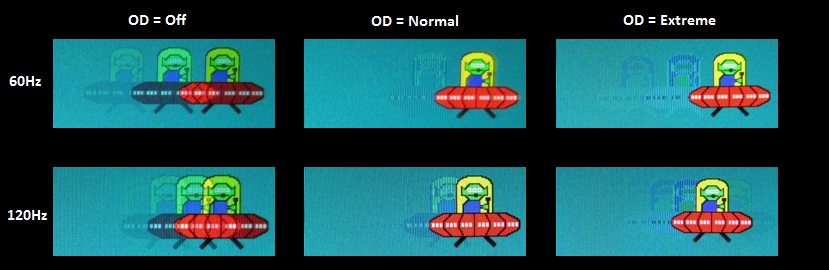
\includegraphics[width=\textwidth]{Applicazione_files/overdrive_ufotest.png}
	\caption{Esempio di artefatti generati dall'\textit{overdrive} dei pixel (da anandtech.com)}
	\label{fig:overdrive_ufotest}
\end{figure}

Non esiste uno standard per la misurazione dell'\textit{overdrive}, quindi in questo test vengono proposti due metodi:\begin{itemize}
	\item \texttt{Assoluto}: considera l'errore sull'intero range di luminosità del display. Ad esempio, se durante una transizione da 16 a 32 si raggiunge un livello di 48, l'\textit{overshoot} è ${\frac{48-32}{255}=6.25\%}$ . Questo è il metodo consigliato
	\item \texttt{Relativo}: considera l'errore relativo al range di luminosità che la transizione deve percorrere. Ad esempio, se durante una transizione da 16 a 32 si raggiunge un livello di 48, l'\textit{overshoot} è  ${\frac{48-32}{32-16}=50\%}$. Questo metodo tende a sovrastimare molto i risultati su transizioni piccole, per cui è quindi generalmente sconsigliato
\end{itemize}

Tra tutti i test implementati nell'applicazione, questo è quello che soffre di più della presenza di rumore, soprattutto retroilluminazione PWM, poiché il test deve misurare delle caratteristiche nel segnale che potrebbero avere una frequenza molto alta. La figura \ref{fig:pixelOverdriveTest_example1} mostra come il segnale potrebbe presentarsi, prima in modo pulito e poi in presenza di PWM. Si può osservare fin da subito che se la frequenza della retroilluminazione PWM è troppo bassa, è completamente impossibile ricostruire il segnale originale, per cui in presenza di retroilluminazione PWM il test tende a sottostimare significativamente l'errore.

Il grafico in figura \ref{fig:pixelOverdriveTest_example2} mostra il segnale ricostruito dall'algoritmo osservando i picchi in presenza di retroilluminazione PWM. Il segnale ricostruito in questo caso ha comunque un picco in corrispondenza dell'\textit{overshoot}, ma è più piccolo e potrebbe essere addirittura assente, per cui non può essere misurato accuratamente dall'applicazione. Le transizioni dal chiaro allo scuro sono più affette da questo problema rispetto a quelle dallo scuro al chiaro.

\begin{figure}[H]
	\centering
	\begin{tikzpicture}
		\begin{axis}[name=Segnale, xmin=0,xmax=0.3,ymin=0,ymax=1023,width=.45\textwidth,xlabel=Tempo (s),ylabel=Valore,xticklabel style={/pgf/number format/fixed}]
			\addplot[black] file{Applicazione_files/pixelOverdriveTest_example_normal.txt};
		\end{axis}
	\end{tikzpicture}
	\begin{tikzpicture}
		\begin{axis}[name=Segnale, xmin=0,xmax=0.3,ymin=0,ymax=1023,width=.45\textwidth,xlabel=Tempo (s),ylabel=Valore,xticklabel style={/pgf/number format/fixed}]
			\addplot[black] file{Applicazione_files/pixelOverdriveTest_example_pwm.txt};
		\end{axis}
	\end{tikzpicture}
	\caption{Segnale senza PWM (sinistra) e segnale con PWM (destra). (Simulato, non è una cattura reale)}
	\label{fig:pixelOverdriveTest_example1}
\end{figure}

\begin{figure}[H]
	\centering
	\begin{tikzpicture}
		\begin{axis}[name=Segnale, xmin=0,xmax=0.5,ymin=0,ymax=1023,width=.7\textwidth,xlabel=Tempo (s),ylabel=Valore,xticklabel style={/pgf/number format/fixed}]
			\addplot[lightgray] file{Applicazione_files/pixelOverdriveTest_example_pwm.txt};
			\addplot[red] file{Applicazione_files/pixelOverdriveTest_example_phf.txt};
		\end{axis}
	\end{tikzpicture}
	\caption{Segnale con PWM (grigio), Segnale filtrato con PeakHoldFilter (rosso). (Simulato, non è una cattura reale)}
	\label{fig:pixelOverdriveTest_example2}
\end{figure}

Il test ha alcuni parametri in input, da passare al costruttore:\begin{itemize}
	\item \texttt{int step}: dimensione del passo tra un livello di luminosità e un altro, sul range 0-255. Si consigliano 16, 32 o 64. Valori più bassi rendono il test più lungo, ma testano più transizioni. (Nota: il valore è espresso nel range 0-255 solo per comodità, internamente vengono convertiti in float nel range 0-1 indipendenti dal formato dei pixel)
	\item \texttt{boolean skipTo0And255}: velocizza il test saltando le transizioni verso 0 e 255, poiché normalmente la luminosità non può scendere sotto il livello di nero, nè sopra il livello di bianco
	\item \texttt{int method}: permette di scegliere tra i due metodi di misurazione (\texttt{METHOD\_ABSOLUTE} o \texttt{METHOD\_RELATIVE})
\end{itemize}

Il seguente pseudocodice mostra il funzionamento del test.
\lstinputlisting{Applicazione_files/PixelOverdriveTest_pseudocode.txt}

Al termine del test, viene chiamato il callback \texttt{onDone} con le seguenti informazioni:\begin{itemize}
	\item \texttt{int[] steps}: array contenente i livelli di luminosità usati nel test come interi nel range 0-255
	\item \texttt{boolean flickeringDetected}: true se il test ha rilevato rumori, come retroilluminazione PWM, che potrebbero ridurre l'accuratezza del test
	\item Molti elementi \texttt{double eFrom>To}: la percentuale di \textit{overshoot}/\textit{undershoot} misurata nella transizione da \texttt{From} a \texttt{To}, dove \texttt{From} e \texttt{To} sono elementi dell'array \texttt{steps}. Sono omessi gli elementi in cui \texttt{From=To}, il cui valore è da considerarsi 0
\end{itemize}

\subsection{Input lag (test interattivo)}
La classe \texttt{InteractiveInputLagTest} implementa un test della latenza totale del sistema, ma a differenza di quello discusso precedentemente, questa è una versione interattiva anziché automatica. A differenza del test automatico, questo test non utilizza affatto un backend grafico: si limita a ricevere i dati dal dispositivo e analizzarli mentre li riceve. Questo test consente di testare il ritardo di input di applicazioni grafiche esterne, in particolar modo videogiochi, in esecuzione sulla stessa macchina o addirittura su una macchina separata.

Il funzionamento del test può essere descritto in modo intuitivo dall'automa a stati finiti in figura \ref{fig:interactiveInputLagTest_fsm}.

\begin{figure}[H]
	\centering
	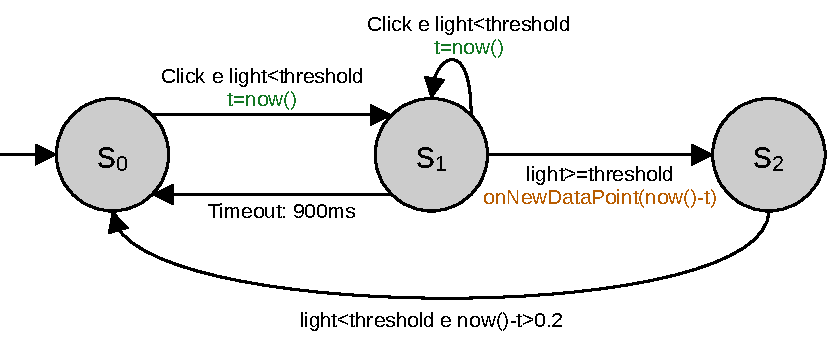
\includegraphics[width=.8\textwidth]{Applicazione_files/interactiveInputLagTest_fsm.pdf}
	\caption{Funzionamento di \texttt{InteractiveInputLagTest}. Le etichette verdi indicano operazioni su variabili, quelle rosse dei callback}
	\label{fig:interactiveInputLagTest_fsm}
\end{figure}

I tre stati hanno i seguenti significati:\begin{itemize}
	\item \textbf{$S_0$}: In attesa del click
	\item \textbf{$S_1$}: Click ricevuto, in attesa del flash
	\item \textbf{$S_2$}: Flash ricevuto, in attesa che finisca
\end{itemize}

All'inizializzazione, è possibile passare al costruttore due istanze di \texttt{IBuffer}, su cui il test scriverà i valori catturati dal sensore di luminosità e dal pulsante, così che sia possibile visualizzarli nell'interfaccia grafica.

Oltre ai metodi dell'interfaccia standard \texttt{ITest}, questa classe implementa anche i seguenti metodi pubblici: \begin{itemize}
	\item \texttt{public abstract void onNewDataPoint(double delay)}: callback che viene chiamato quando è disponibile un nuovo dato sulla latenza. Il parametro \texttt{delay} contiene il tempo in millisecondi trascorso tra il click e il flash. Attenzione: questo metodo deve terminare il prima possibile per evitare di rallentare il campionamento
	\item \texttt{public void setThreshold(int threshold)}: permette di impostare la soglia di rilevazione del flash come intero tra 0 e 1023
	\item \texttt{public int getThreshold()}: ritorna la soglia di rilevazione del flash corrente come intero tra 0 e 1023. Il valore di default è 100
	\item \texttt{public void setSensitivity(byte sensitivity)}: imposta la sensibilità del sensore tra i quattro valori possibili (0=minima, 3=massima)
	\item \texttt{public byte getSensitivity()}: ritorna la sensibilità attuale del sensore. Il valore di default è 2
	\item \texttt{public void setAutoFire(boolean autoFire)}: permette di attivare o disattivare la generazione automatica dei click anziché utilizzare il pulsante esterno
	\item \texttt{public boolean getAutoFire()}: ritorna \texttt{true} se il dispositivo sta generando i click, false se li riceve dal pulsante esterno. Di default li riceve dall'esterno. Il valore di default è \texttt{false}
	\item \texttt{public byte getState()}: ritorna lo stato attuale dell'automa in figura \ref{fig:interactiveInputLagTest_fsm}
\end{itemize}

Il test prosegue indefinitamente fino a quando non viene terminato manualmente dall'utente chiamando il metodo \texttt{onCancel}. Il callback \texttt{onDone} viene comunque chiamato alla terminazione ma non gli viene passato nessun dato.

Il test può essere utilizzato in due modi:\begin{itemize}
	\item \textbf{Sulla stessa macchina}: in questo caso è sufficiente avviare il test e attivare la generazione automatica dei click. Il dispositivo genera click a una frequenza di circa 1 click al secondo, e posizionando il dispositivo in corrispondenza del \textit{muzzle flash} di un'arma o qualche altro elemento del gioco che genera un flash in risposta ai click, è possibile misurare quanto tempo passa tra un click e la generazione del flash
	\item \textbf{Su una macchina separata}: si avvia il test utilizzando come fonte dei click il pulsante esterno, si collegano i pin del pulsante esterno ad un mouse o appositamente modificato come spiegato nel capitolo precedente sull'hardware, si posiziona il sensore sul display della macchina da testare come nel caso precedente e il test misura il tempo che passa tra la pressione del pulsante e la generazione del flash. Si consiglia di far passare almeno mezzo secondo tra un click e l'altro
\end{itemize}

Durante il test, è possibile regolare manualmente la soglia di rilevazione del flash e la sensibilità del sensore. La soglia di rilevazione deve essere impostata il più bassa possibile, ma alta abbastanza da non attivarsi accidentalmente. Per risultati migliori, è consigliabile posizionarsi in un'area scura e utilizzare un'arma o un altro elemento del gioco che genera un flash immediatamente quando viene premuto il pulsante, senza eseguire un'animazione prima.

\subsection{Light to sound}
La classe \texttt{InteractiveLightToSound} implementa un altro test interattivo, che consente di ascoltare il segnale catturato dal dispositivo. Pur non producendo alcun risultato, questo test consente di puntare il dispositivo verso lampadine o altri dispositivi luminosi e sentire immediatamente se la luce è stabile o se ha disturbi. Nel caso delle lampadine, i disturbi sono principalmente causati da un circuito di rettificazione e filtraggio dell'alimentazione inadeguato che causa un \textit{flickering} a 50 o 100Hz più o meno visibile, che a lungo termine può affaticare la vista.\\
Il test è implementato utilizzando le classi dell'audio \texttt{javax.sound.sampled}. Durante il test, è possibile variare il volume dell'output e la sensibilità del sensore.

Oltre ai metodi dell'interfaccia standard \texttt{ITest}, questa classe implementa anche i seguenti metodi pubblici: \begin{itemize}
	\item \texttt{public void setSensitivity(byte sensitivity)}: imposta la sensibilità del sensore tra i quattro valori possibili (0=minima, 3=massima)
	\item \texttt{public byte getSensitivity()}: ritorna la sensibilità attuale del sensore. Il valore di default è 2
	\item \texttt{public void setVolume(int volume)}: imposta il volume dell'output come un numero tra 0 e 1
	\item \texttt{public float getVolume()}: ritorna il volume corrente. Il valore di default è 1
	\item \texttt{public double getSampleRate()}: ritorna il sample rate in Hz
	\item \texttt{public IBuffer getChartBuffer()}: ritorna un'istanza di \texttt{CircularBuffer} contenente l'ultimo mezzo secondo di audio, così che sia possibile visualizzarlo nell'interfaccia grafica. Il contenuto del buffer ritornato è sempre aggiornato, non è necessario riottenerlo ogni volta che serve
	\item \texttt{public double getStrongestFrequency(double from, double to)}: ritorna la frequenza in Hz più forte nel range specificato, oppure -1 se non ce ne sono o sono troppo deboli per essere rilevanti
\end{itemize}

Il test prosegue indefinitamente fino a quando non viene terminato manualmente dall'utente chiamando il metodo \texttt{onCancel}. Il callback \texttt{onDone} viene comunque chiamato alla terminazione ma non gli viene passato nessun dato.

%RIMOSSO PER DUBBIA UTILITÀ, meglio metterlo nella documentazione
%\subsection{Template per test automatici}
%Il seguente listato mostra il codice minimo per eseguire un test automatico utilizzando i backend grafici forniti e un thread eseguire per il test.
%
%\lstinputlisting[language=Java]{Applicazione_files/TestExample.java}
%
Questo conclude la sezione dedicata all'implementazione dei test.

\section{Interfaccia grafica}
Questa sezione è dedicata all'interfaccia grafica dell'applicazione OpenLDAT, implementata nel package \texttt{com.dosse.openldat.ui}.

L'interfaccia è stata sviluppata utilizzando le librerie Swing di Java SE con alcuni accorgimenti per supportare i display con DPI alti, e permette di avviare i test e visualizzarne i risultati in maniera semplice e intuitiva. Non c'è nulla di particolarmente interessante dal punto di vista tecnico nell'implementazione della GUI, per cui questa sezione si concentra principalmente sulle funzionalità e l'utilizzo dell'interfaccia grafica.

Attualmente non sono implementate localizzazioni, l'interfaccia è disponibile solo in lingua Inglese.

L'interfaccia è pensata per essere utilizzata con un mouse, ma è presente un supporto limitato per i touchscreen e la navigazione da tastiera.

\subsection{Selezione del dispositivo}
All'avvio dell'applicazione viene scansionato il PC per trovare dispositivi OpenLDAT connessi. Se viene trovato più di un dispositivo, viene mostrata una schermata di selezione come quella in figura \ref{fig:gui_deviceSelector} da cui è possibile distinguerli in base alla porta a cui sono collegati. Se c'è un solo dispositivo questa schermata viene saltata.

\begin{figure}[h]
	\centering
	\includegraphics[width=.5\textwidth]{Applicazione_files/gui_deviceSelector.png}
	\caption{Selezione del dispositivo}
	\label{fig:gui_deviceSelector}
\end{figure}

Premendo il pulsante \textit{Connect} si avvia l'applicazione utilizzando il dispositivo selezionato, premendo \textit{Refresh} è possibile rieseguire la scansione.

\subsection{Menu principale}
Dopo la selezione del dispositivo, viene visualizzato il menu principale dell'applicazione come in figura \ref{fig:gui_mainMenu2}. Questa schermata è divisa in due parti: a sinistra sono elencati tutti i test e le funzioni dell'applicazione, sulla destra è presente un manuale che mostra informazioni sul test selezionato e il pulsante per avviarlo. Le pagine del manuale mostrato sulla destra sono memorizzate come dei file HTML nella cartella \texttt{manual} all'interno del package della GUI.

\begin{figure}[h]
	\centering
	\includegraphics[width=\textwidth]{Applicazione_files/gui_mainMenu2.png}
	\caption{Menu principale con un test selezionato}
	\label{fig:gui_mainMenu2}
\end{figure}

Il menu principale fornisce accesso alle seguenti funzioni:\begin{itemize}
	\item \textbf{Welcome}: mostra una schermata di benvenuto con alcuni suggerimenti generali per l'utilizzo corretto dei test
	\item \textbf{Input Lag (Automated test)}: esegue il test automatico del ritardo di input
	\item \textbf{Input Lag (Manual test)}: esegue il test interattivo del ritardo di input
	\item \textbf{Microstuttering detection}: esegue il test di rilevamento del \textit{microstuttering}
	\item \textbf{PWM/Strobing test}: esegue il test di rilevamento PWM e altri rumori
	\item \textbf{Pixel Response Time}: esegue il test che misura il tempo di risposta dei pixel tra diverse sfumature di grigio
	\item \textbf{Pixel Overdrive (Overshoot/Undershoot)}: esegue il test che misura l'errore di transizione causato dall'\textit{overdrive} dei pixel
	\item \textbf{Light To Sound}: avvia la modalità Light To Sound, per ascoltare i dati catturati dal sensore di luminosità
	\item \textbf{Driver test}: fornisce accesso a un pannello da cui è possibile testare tutte le funzioni del dispositivo, del driver e dell'elaborazione di base
	\item \textbf{Advanced settings}: permette di cambiare alcune impostazioni dell'applicazione che normalmente sono determinate automaticamente
	\item \textbf{About OpenLDAT}: mostra informazioni sull'applicazione
\end{itemize}

\subsection{Test automatici}
I test automatici seguono tutti i seguenti passi quando vengono avviati:\begin{itemize}
	\item Se il test ha dei parametri configurabili, mostra una schermata di configurazione
	\item Esegui il test
	\item Mostra una schermata con i risultati
	\item Torna al menu principale
\end{itemize}

\subsubsection{Input lag (test automatico)}
Questo test ha dei parametri che possono essere configurati, mostrati in figura \ref{fig:gui_inputlag_settings}:\begin{itemize}
	\item \textbf{VSync mode}: permette di attivare o disattivare il \textit{VSync}
	\item \textbf{Fake CPU load}: simula la presenza di carico sulla CPU durante l'esecuzione del test. Il carico è espresso in millisecondi per frame
	\item \textbf{Fake GPU load}: simula la presenza di carico sulla GPU durante l'esecuzione del test. Il carico è espresso in millisecondi per frame
	\item \textbf{Test duration}: permette di selezionare la durata del test tra 20 secondi, 1 minuto (default), 2 minuti o 5 minuti. Test più lunghi garantiscono risultati più accurati
\end{itemize}

Al termine del test, viene visualizzata una schermata con i risultati come in figura \ref{fig:gui_inputlag_results}. Da qui è possibile salvarli su un file importabile in un foglio di calcolo oppure tornare al menu principale.

\begin{figure}[H]
	\centering
	\includegraphics[width=.8\textwidth]{Applicazione_files/gui_inputlag_settings.png}
	\caption{Input lag: impostazioni del test}
	\label{fig:gui_inputlag_settings}
\end{figure}

\begin{figure}[H]
	\centering
	\includegraphics[width=\textwidth]{Applicazione_files/gui_inputlag_results.png}
	\caption{Input lag: risultati del test}
	\label{fig:gui_inputlag_results}
\end{figure}

\subsubsection{Rilevamento del microstuttering}
Questo test non ha parametri da configurare, per cui viene eseguito immediatamente. Al termine viene mostrata una schermata con i risultati come in figura \ref{fig:gui_microstuttering_results}. Da qui è possibile salvarli su un file importabile in un foglio di calcolo oppure tornare al menu principale. La presenza di picchi sopra la linea rossa nel grafico indica la presenza di \textit{microstuttering}.

Nota: è stato osservato che su alcune piattaforme, il backend Swing, non essendo in grado di sincronizzarsi con il display, può generare esso stesso \textit{microstuttering}; per questo motivo, al fine di evitare di fornire dati potenzialmente errati, è stato scelto di far funzionare questo test solo con il backend OpenGL. Il codice del test supporta entrambi i backend, la restrizione è presente solo nel codice della GUI che avvia il test.

\begin{figure}[H]
	\centering
	\includegraphics[width=\textwidth]{Applicazione_files/gui_microstuttering_results.png}
	\caption{Rilevamento del \textit{microstuttering}: risultati del test}
	\label{fig:gui_microstuttering_results}
\end{figure}

\subsubsection{Rilevamento di PWM e noise}
Questo test non ha parametri da configurare, per cui viene eseguito immediatamente. Al termine viene mostrata una schermata con i risultati come in figura \ref{fig:gui_pwm_results}. Da qui è possibile salvarli su un file importabile in un foglio di calcolo oppure tornare al menu principale. Il grafico mostra il segnale catturato dal sensore durante il test.

\begin{figure}[H]
	\centering
	\includegraphics[width=\textwidth]{Applicazione_files/gui_pwm_results.png}
	\caption{Rilevamento di PWM e noise: risultati del test su un display con una pessima retroilluminazione}
	\label{fig:gui_pwm_results}
\end{figure}

\subsubsection{Tempi di risposta dei pixel}
Questo test ha due parametri che possono essere configurati, mostrati in figura \ref{fig:gui_pixelresponse_settings}:\begin{itemize}
	\item \textbf{Evaluation method}: permette di scegliere il range della transizione di cui misurare il tempo. Lo standard VESA prevede di misurare il tempo richiesto per la transizione dal 10\% al 90\%, per cui questo è il default, ma può essere selezionata anche un'altra modalità chiamata umoristicamente ``BS Manufactures Say'' per misurare il range 30\%-70\%, che è più tipicamente usato dai produttori di schermi ``da gaming''
	\item \textbf{Step size}: il passo tra due sfumature di grigio. Valori più piccoli testano più sfumature di grigio ma rendono il test molto più lungo. I valori implementati sono 16 (lento), 32 (default) e 64 (veloce). Questi valori sono su una scala tra 0 e 255 solo per comodità, il test utilizza il formato dei pixel del desktop
\end{itemize}

Al termine del test, viene visualizzata una schermata con i risultati come in figura \ref{fig:gui_pixelresponse_results}. Da qui è possibile salvarli su un file importabile in un foglio di calcolo oppure tornare al menu principale. I colori nella tabella indicano in modo intuitivo quanto è buono il tempo di quella transizione con una sfumatura dal verde al rosso.

Nota: i valori di luminosità sono su una scala tra 0 e 255 solo per comodità, il test utilizza il formato dei pixel del desktop.

\begin{figure}[H]
	\centering
	\includegraphics[width=.8\textwidth]{Applicazione_files/gui_pixelresponse_settings.png}
	\caption{Tempi di risposta dei pixel: impostazioni del test}
	\label{fig:gui_pixelresponse_settings}
\end{figure}

\begin{figure}[H]
	\centering
	\includegraphics[width=\textwidth]{Applicazione_files/gui_pixelresponse_results.png}
	\caption{Tempi di risposta dei pixel: risultati del test}
	\label{fig:gui_pixelresponse_results}
\end{figure}

\subsubsection{Overdrive dei pixel}
Questo test ha tre parametri che possono essere configurati, mostrati in figura \ref{fig:gui_pixeloverdrive_settings}:\begin{itemize}
	\item \textbf{Method}: permette di scegliere il metodo di misurazione tra Relativo e Assoluto (default), il cui significato è approfondito nella sezione dedicata al funzionamento di questo test
	\item \textbf{Step size}: il passo tra due sfumature di grigio. Valori più piccoli testano più sfumature di grigio ma rendono il test molto più lungo. I valori implementati sono 16 (lento), 32 (default) e 64 (veloce). Questi valori sono su una scala tra 0 e 255 solo per comodità, il test utilizza il formato dei pixel del desktop
	\item \textbf{Skip transitions to 0 and 255}: velocizza il test saltando le transizioni verso il nero e verso il bianco, dato che normalmente il display non può visualizzare colori più scuri del nero o più chiari del bianco
\end{itemize}

Al termine del test, viene visualizzata una schermata con i risultati come in figura \ref{fig:gui_pixeloverdrive_results}. Da qui è possibile salvarli su un file importabile in un foglio di calcolo oppure tornare al menu principale. I colori nella tabella indicano in modo intuitivo quanto è buono il tempo di quella transizione con una sfumatura dal verde al rosso.

Attenzione: questo test è estremamente sensibile alla presenza di PWM o altri disturbi.

Nota: i valori di luminosità sono su una scala tra 0 e 255 solo per comodità, il test utilizza il formato dei pixel del desktop.

\begin{figure}[H]
	\centering
	\includegraphics[width=.8\textwidth]{Applicazione_files/gui_pixeloverdrive_settings.png}
	\caption{Overdrive dei pixel: impostazioni del test}
	\label{fig:gui_pixeloverdrive_settings}
\end{figure}

\begin{figure}[H]
	\centering
	\includegraphics[width=\textwidth]{Applicazione_files/gui_pixeloverdrive_results.png}
	\caption{Overdrive dei pixel: risultati del test}
	\label{fig:gui_pixeloverdrive_results}
\end{figure}

\subsection{Test interattivi}
I test interattivi mostrano una schermata di test in cui è possibile configurarlo mentre il test è in esecuzione. Questi test procedono indefinitamente fino a quando non vengono interrotti dall'utente.

\subsubsection{Input lag (test interattivo)}
Questo test permette di misurare il ritardo in risposta ai click di virtualmente qualsiasi applicazione.

L'interfaccia grafica del test (figura \ref{fig:gui_interactiveinputlag_results}) è organizzata in questo modo:\begin{itemize}
	\item Il grafico mostra i dati del sensore di luminosità (bianco), i click (azzurro) e la soglia di attivazione (linea verde orizzontale)
	\item Alla destra del grafico è possibile regolare la soglia di attivazione con il cursore
	\item Sotto al grafico, sulla destra è possibile cambiare il gain del sensore tra i quattro livelli disponibili e scegliere se i click devono essere generati automaticamente dal dispositivo o se devono essere ricevuti dall'esterno (default)
	\item Sotto al grafico, a sinistra è presente un elenco di tempi misurati finora con la relativa media e la possibilità di salvare i tempi su file e di resettare il test qualora siano stati catturati dati errati
\end{itemize}

\begin{figure}[H]
	\centering
	\includegraphics[width=\textwidth]{Applicazione_files/gui_interactiveinputlag_results.png}
	\caption{Input lag (test interattivo): schermata di test}
	\label{fig:gui_interactiveinputlag_results}
\end{figure}

\subsubsection{Light to sound}
Quest'ultimo test permette di ascoltare il segnale del sensore di luminosità come audio.

L'interfaccia grafica del test (figura \ref{fig:gui_lighttosound_results}) è organizzata in questo modo:\begin{itemize}
	\item Il grafico mostra l'ultimo mezzo secondo del segnale catturato
	\item I controlli sotto al grafico permettono di regolare il volume dell'audio e il livello di gain del sensore
	\item Quando viene rilevata una frequenza sufficientemente potente (ad esempio da una retroilluminazione PWM), questa viene mostrata sotto ai controlli
	\item In basso a sinistra viene mostrato il sample rate del segnale catturato
\end{itemize}

\begin{figure}[H]
	\centering
	\includegraphics[width=\textwidth]{Applicazione_files/gui_lighttosound_results.png}
	\caption{Light to sound: schermata di test}
	\label{fig:gui_lighttosound_results}
\end{figure}

\subsection{Impostazioni}
La schermata delle impostazioni mostrata in figura \ref{fig:gui_settings} permette di cambiare alcune impostazioni che l'applicazione determina automaticamente:\begin{itemize}
	\item \textbf{Graphics backend}: seleziona il backend grafico tra OpenGL e Swing. Di default viene usato OpenGL se è disponibile, Swing è usato solo come fallback
	\item \textbf{Use antialiasing on charts (slower)}: migliora la qualità dei grafici disegnandoli con l'\textit{antialiasing}. Di default è disattivato
	\item \textbf{Disable X11 hacks}: permette di disattivare alcune ottimizzazioni che aumentano la stabilità dell'applicazione su X11 (solo per GNU/Linux). Di default è disattivato
\end{itemize}

Queste impostazioni sono rese disponibili a tutte le classi dell'applicazione sotto forma di variabili statiche nella classe \texttt{Config}, la quale si occupa anche di memorizzarle su disco e applicarle anche ai successivi utilizzi. Le impostazioni sono memorizzate nella cartella \texttt{\textasciitilde/.openldat} (GNU/Linux e MacOS) o \texttt{\%USERPROFILE\%\textbackslash.openldat} (Windows).

\begin{figure}[H]
	\centering
	\includegraphics[width=.8\textwidth]{Applicazione_files/gui_settings.png}
	\caption{Impostazioni dell'applicazione}
	\label{fig:gui_settings}
\end{figure}

\subsection{Schermata about}
Questa schermata mostra le informazioni sull'applicazione: versione, copyright e licenza (GNU GPL Versione 3).

\begin{figure}[H]
	\centering
	\includegraphics[width=.8\textwidth]{Applicazione_files/gui_about.png}
	\caption{Informazioni su OpenLDAT}
	\label{fig:gui_about}
\end{figure}

Facendo click ripetutamente sul logo di OpenLDAT per 7 volte è possibile accedere al Driver test anche su dispositivi che non sono marcati come prototipi.

\subsection{Gestore grafico degli errori}
L'ultimo componente della GUI è il gestore degli errori. La classe \texttt{ErrorDialog} implementa la schermata di errore in figura \ref{fig:gui_errordialog} e può gestire i seguenti errori:\begin{itemize}
	\item \textbf{Errori dell'applicazione}: file corrotti, applicazione già avviata, crash di thread, eccetera. Questi errori sono critici e causano la chiusura dell'applicazione
	\item \textbf{Errori del dispositivo e del driver}: dispositivi non supportati, disconnessioni inaspettate, risposte non valide del firmware, eccetera. Questi errori sono critici e causano la chiusura dell'applicazione
	\item \textbf{Errori dei test}: fallimenti nell'analisi, contrasto insufficiente, problemi con il backend grafico, sensori mancanti, eccetera. Questi errori causano il fallimento del test, ma l'applicazione può continuare. Alcuni di questi errori, per esempio l'annullamento del test da parte dell'utente, non causano la visualizzazione di un messaggio d'errore
\end{itemize}

\begin{figure}[H]
	\centering
	\includegraphics[width=.8\textwidth]{Applicazione_files/gui_errordialog.png}
	\caption{Schermata di errore di OpenLDAT}
	\label{fig:gui_errordialog}
\end{figure}

Un errore che viene trattato in modo speciale da questa classe è quello che si verifica se il dispositivo viene rilevato ma l'utente corrente non ha i permessi per comunicare con esso. Questo è un problema che si verifica su alcune distribuzioni di GNU/Linux e l'applicazione implementa una schermata di errore speciale (figura \ref{fig:gui_linuxerror}) che si offre di correggere i permessi automaticamente tramite uno script (se l'utente è amministratore) o di mostrare istruzioni su come farlo manualmente da un terminale.\\
Lo script automatico supporta distribuzioni GNU/Linux basate su Debian, Arch, SUSE e RedHat, ed è stato testato su Ubuntu 21.04, Debian 10.9, Manjaro 21, Arch Linux (Aprile 2021), OpenSUSE 15, Fedora 34.

\begin{figure}[H]
	\centering
	\includegraphics[width=\textwidth]{Applicazione_files/gui_linuxerror.png}
	\caption{Correzione automatica dei permessi mancanti su GNU/Linux}
	\label{fig:gui_linuxerror}
\end{figure}

Questo conclude la sezione di presentazione dell'interfaccia grafica dell'applicazione OpenLDAT.

\section{Packaging dell'applicazione}
Per consentire un facile utilizzo dell'applicazione, soprattutto da utenti inesperti, è necessario creare dei pacchetti binari per le varie piattaforme. Sono stati scelte le seguenti piattaforme:\begin{itemize}
	\item Windows 10 x64
	\item GNU/Linux amd64 (diverse distribuzioni popolari)
	\item MacOS Intel 64 bit
\end{itemize}
Essendo il codice multipiattaforma, è possibile utilizzarlo anche su altre piattaforme come BSD o Windows a 32 bit, tuttavia queste non sono state testate e non si garantisce il corretto funzionamento.

Tutti i file e le istruzioni necessarie per generare i pacchetti sulle piattaforme supportate sono presenti nella cartella \texttt{Packaging stuff} all'interno della cartella dell'applicazione.

\subsection{Windows}
Il pacchetto di installazione per Windows è stato realizzato utilizzando Inno Setup\footnote{\url{https://jrsoftware.org/isinfo.php}}. All'interno del package sono presenti l'applicazione OpenLDAT con le relative librerie, il runtime Java (OpenJDK 11 JRE\footnote{\url{https://adoptopenjdk.net/releases.html}}) e un launcher eseguibile per Windows realizzato con Launch4J\footnote{\url{https://launch4j.sourceforge.net/}}.

La procedura per realizzare il package è la seguente:\begin{itemize}
	\item Fare una copia della cartella \texttt{Windows-InnoSetup}
	\item Eseguire la build del progetto OpenLDAT da NetBeans IDE
	\item Dalla cartella \texttt{dist} nel progetto appena compilato, copiare \texttt{OpenLDAT.jar} e la cartella \texttt{lib} nella cartella \texttt{openldat}
	\item Scaricare il file zip di OpenJDK JRE x64 versione 11 o superiore dal relativo sito
	\item All'interno dello zip scaricato estrarre i file del runtime (cartelle \texttt{bin}, \texttt{lib}, eccetera) nella cartella \texttt{jre}
	\item Utilizzando Launch4J, eseguire la build del file \texttt{launcher.xml}
	\item Utilizzando Inno Setup 6, eseguire la build del file \texttt{setup.iss}. Al termine verrà generato un file chiamato \texttt{OpenLDAT\_Setup.exe} che può essere distribuito. Si consiglia di firmarlo digitalmente
\end{itemize}

\subsection{GNU/Linux}
Il pacchetto per GNU/Linux è distribuito nel formato AppImage\footnote{\url{https://appimage.org/}}, che non richiede installazione. All'interno del package sono presenti l'applicazione OpenLDAT con le relative librerie e il runtime Java (OpenJDK 11 JRE).

La procedura per realizzare il package è la seguente:\begin{itemize}
	\item Fare una copia della cartella \texttt{Linux-AppImage} ed entrare nella cartella \texttt{OpenLDAT.AppDir}
	\item Eseguire la build del progetto OpenLDAT da NetBeans IDE
	\item Dalla cartella \texttt{dist} nel progetto appena compilato, copiare \texttt{OpenLDAT.jar} e la cartella \texttt{lib} nella cartella \texttt{openldat}
	\item Scaricare il file zip di OpenJDK JRE x64 versione 11 o superiore dal relativo sito
	\item All'interno dello zip scaricato estrarre i file del runtime (cartelle \texttt{bin}, \texttt{lib}, eccetera) nella cartella \texttt{jre}
	\item Tornare al livello superiore ed eseguire il seguente comando:\begin{verbatim}
		appimagetool OpenLDAT.AppDir
	\end{verbatim}
	Al termine verrà generato un file chiamato \texttt{OpenLDAT-x86\_64.AppImage} che può essere distribuito
\end{itemize}

\subsection{MacOS}
Il pacchetto per MacOS è distribuito sotto forma di immagine DMG contenente un'applicazione nel formato standard .app, la quale contiene al suo interno l'applicazione OpenLDAT con le relative librerie, il runtime Java (OpenJDK 11 JRE) e un wrapper per consentire l'avvio di applicazioni Java su MacOS\footnote{\url{https://github.com/tofi86/universalJavaApplicationStub}}.

Nota: il testing su questa piattaforma è stato estremamente limitato e non è stato eseguito dall'autore di questa tesi.

La procedura per realizzare il package è la seguente:\begin{itemize}
	\item Fare una copia della cartella \texttt{Mac}
	\item Eseguire la build del progetto OpenLDAT da NetBeans IDE
	\item Dalla cartella \texttt{dist} nel progetto appena compilato, copiare \texttt{OpenLDAT.jar} e la cartella \texttt{lib} nella cartella \texttt{openldat}
	\item Scaricare il file zip di OpenJDK JRE x64 versione 11 dal relativo sito\\
	Attenzione: La versione 11 è l'unica supportata da questo sistema di packaging al momento
	\item All'interno dello zip scaricato estrarre i file del runtime (cartelle \texttt{bin}, \texttt{lib}, eccetera) nella cartella \texttt{jre/openjdk-11-jre}
	\item Eseguire lo script \texttt{makeapp}. Al termine verrà generata una cartella \texttt{OpenLDAT.app}
	\item Utilizzare Disk Utility per creare un'immagine DMG compressa contenente \texttt{OpenLDAT.app} che può essere distribuita
\end{itemize}

Questo conclude il capitolo sull'applicazione OpenLDAT per PC. Nel capitolo successivo verranno mostrati e discussi alcuni risultati raccolti con l'applicazione e il dispositivo in diversi scenari.

\newpage
\chapter{Risultati sperimentali}
\label{chap:expdata}

Questo capitolo è dedicato ai risultati che sono stati ottenuti testando il dispositivo e l'applicazione su diversi tipi di display e configurazioni hardware e software.

Al fine di raccogliere un campione di dimensione sufficienti, oltre ai display che erano a disposizione dell'autore di questa tesi, sono stati realizzati due prototipi che sono stati prestati a varie persone al fine di poter aggiungere i risultati dei loro display. Idealmente sarebbe stato preferibile testare tutti i display personalmente e sulla stessa macchina, ma le condizioni causate dalla pandemia durante i primi mesi del 2021 non lo consentivano, per cui alcuni test sono stati svolti da terzi con istruzioni in videoconferenza, ma comunque su macchine volutamente simili. Idealmente tutti i test andrebbero ripetuti in un ambiente controllato, per avere dati più confrontabili.

La tabella \ref{tab:display_list} mostra l'elenco di tutti i dispositivi che sono stati testati e le loro caratteristiche salienti. Non tutti i dispositivi appariranno in tutti i test. Sono stati eseguiti i seguenti test:\begin{itemize}
	\item \textbf{Input lag}:\begin{itemize}
		\item Confronto tra diversi display
		\item Confronto tra sistemi operativi, GPU e driver
		\item Confronto tra tipi di \textit{VSync}
		\item Confronto tra diverse applicazioni utilizzando il test manuale
		\item Validazione dei risultati con telecamera ad alta velocità
	\end{itemize}
	\item \textbf{PWM e noise}: confronto tra diversi display e dimostrazione dei diversi tipi di rumore che possono essere presenti sul segnale
	\item \textbf{Microstuttering}: confronto tra diversi display a \textit{refresh rate} nativo e in \textit{overclock}
	\item \textbf{Tempi di risposta e \textit{overdrive} dei pixel}:\begin{itemize}
		\item Confronto dei tempi di risposta tra display diversi, con e senza \textit{overdrive}
		\item Confronto degli errori di transizione commessi dai display con e senza \textit{overdrive}
	\end{itemize}
\end{itemize}

In tutti i casi i display sono stati impostati alle impostazioni di fabbrica, e sono state disattivate tutte le migliorie all'immagine nelle impostazioni del display che potrebbero interferire con i test, in particolar modo contrasto dinamico e \textit{black frame insertion}. Il segnale video utilizzato per i test è sempre stato \textit{full range RGB} a 8 bit o 10 bit ove supportato.

Nelle sezioni successive, per ogni test, verranno introdotte le modalità di testing, delle tabelle e grafici riassuntivi dei valori ottenuti, e alcune riflessioni sui risultati ottenuti.

\begin{landscape}
\begin{table}[h!]
	\centering
		\begin{tabular}{|l|c|c|c|c|c|c|} 
			\hline
			\textbf{Dispositivo} & \textbf{Tipo} & \textbf{Anno} & \textbf{Refresh} & \textbf{Tecnologia} & \textbf{Retroilluminazione} & \textbf{Testato da}  \\ 
			\hline
			Acer Predator XB271HU & Monitor & 2019 & 165Hz VRR & TN  & Edge LED & Terzi \\ \hline
			Acer Swift 3 & Laptop & 2020 & 60Hz & IPS & Edge LED & Autore \\ \hline
			AOC Q2770P & Monitor & 2014 & 60Hz & IPS & Edge LED & Autore \\ \hline
			ASUS VP228HE & Monitor & 2019 & 60Hz & TN & Edge LED & Terzi \\ \hline
			ASUS VW228 & Monitor & 2011 & 60Hz & TN & Edge LED & Terzi \\ \hline
			BenQ GL2706PQ & Monitor & 2014 & 60Hz & TN & Edge LED & Terzi \\ \hline
			BenQ XL2420T & Monitor & 2012 & 120Hz & TN & Edge LED & Terzi \\ \hline
			Huawei MateBook D & Laptop & 2019 & 60Hz & IPS & Edge LED & Terzi \\ \hline
			iPhone 6S & Smartphone & 2015 & 60Hz & IPS & Edge LED & Terzi \\ \hline
			LG 27GL850-B & Monitor & 2018 & 144Hz VRR & IPS HDR & Edge LED & Terzi \\ \hline
			LG E2360 & Monitor & 2012 & 60Hz & TN & Edge LED & Terzi \\ \hline
			MacBook Pro 13" & Laptop & 2017 & 60Hz & IPS & Edge LED & Terzi \\ \hline
			Octigen M19W & Monitor & 2008 & 60Hz & TN & CCFL & Autore \\ \hline
			OnePlus 3T & Smartphone & 2016 & 60Hz & AMOLED & N/A & Autore \\ \hline
			OnePlus 7 Pro & Smartphone & 2019 & 90Hz VRR & AMOLED & N/A & Terzi \\ \hline
			Philips 32PFS4132 & TV & 2020 & 60Hz & TN & Edge LED & Autore \\ \hline
			Philips 105MB & Monitor & 1997 & N/A & CRT & N/A & Autore \\ \hline
			Samsung C34H890 & Monitor & 2019 & 100Hz VRR & VA & LED Array & Terzi \\ \hline
			Samsung P2770HD & TV & 2011 & 60Hz & TN & Edge LED & Autore \\ \hline
			Sony VAIO SVF1532C5E & Laptop & 2014 & 60Hz & TN & Edge LED & Terzi \\ \hline
			Sharp Aquos LC-40FG3242E & TV & 2020 & 60Hz & TN & Edge LED & Autore \\ \hline
			Thinkpad T480 & Laptop & 2018 & 60Hz & IPS & Edge LED & Autore \\ \hline
		\end{tabular}
	\caption{\label{tab:display_list}Lista completa dei dispositivi testati}
\end{table}
\end{landscape}

\section{Input lag}
In questa sezione vengono utilizzati i test dell'applicazione OpenLDAT per determinare l'\textit{input lag} di diversi display, e vedere come questo è influenzato dalla configurazione hardware e software.

Sono stati eseguiti i seguenti test:\begin{itemize}
	\item Confronto tra diversi display
	\item Confronto tra sistemi operativi, GPU e driver
	\item Confronto tra modalità di \textit{VSync} nel test automatico
	\item Confronto tra diverse applicazioni utilizzando il test manuale
	\item Validazione dei risultati con telecamera ad alta velocità
\end{itemize}

\subsection{Confronto tra display}
In questo test è stato misurato il ritardo dei display utilizzando il test automatico dell'applicazione OpenLDAT. Il test è stato eseguito con e senza \textit{VSync}, utilizzando il backend grafico OpenGL a risoluzione nativa. Al fine di avere dei risultati il più confrontabili possibile, tutti i test sono stati eseguiti su Windows 10 con una GPU Nvidia, ad eccezione dei laptop per cui è stato possibile utilizzare solo la grafica integrata Intel. In tutti i casi, i display sono stati collegati tramite un'interfaccia digitale (HDMI o DP), ad eccezione del Philips 105MB e dell'Octigen M19W che hanno solo un'ingresso VGA.

\begin{figure}[h!]
	\centering
	\pgfplotstableread[col sep=comma]{
		model,novsync,vsync
		Acer Predator XB271HU (165Hz G-Sync),6.3,32.5
		LG 27GL850-B (144Hz Freesync),6.4,36.9
		BenQ XL2420T (120Hz),9.2,44.1
		%Huawei Matebook D 2019 (60Hz Laptop),10.1,86.3 %dubito dell'accuratezza di questo risultato, sembra troppo basso il vsync off, probabilmente il tizio si è mosso durante il test
		Samsung C34H890 (100Hz Freesync),11.8,52.8
		Philips 105MB (85Hz CRT),13.1,64.2
		ASUS VP228HE (60Hz),13.1,86.8
		LG E2360 (60Hz),14.1,89.6
		Sony VAIO SVF1532C5E (60Hz Laptop),15.5,62.4
		ASUS VW228 (60Hz),16.0,88.5
		Thinkpad T480 2018 (60Hz Laptop),18.2,88.8
		Octigen M19W (60Hz),19.6,88.2
		BenQ GL2706PQ (60Hz),27.7,93.7
		AOC Q2770P (60Hz),29.8,95.8
		MacBook Pro 13" 2017 (60Hz Laptop),30.2,96.7
		Acer Swift 3 (60Hz Laptop),31.8,111.2
		Philips 32PFS4132 (60Hz TV),34.9,106.5
		Sharp LC-40FG3242E (60Hz TV),37.1,108.8
		Samsung P2770HD (60Hz TV),41.1,111.9
	}\dataset
	\begin{tikzpicture}
		\begin{axis}[xbar, bar width=8pt, y dir=reverse, ytick=data, yticklabels from table={\dataset}{model}, yticklabel style={text width=3.5cm, align=right}, table/y expr = \coordindex, nodes near coords, reverse legend, legend style={at={(0.5,-1.1cm)},anchor=north}, xlabel=Ritardo (ms), width=\textwidth-3cm, height=18cm, xmin=0, ymin=-1, ymax=18] %ymax messo a mano con il numero di display per migliore formattazione
			\addplot table[x=vsync] {\dataset};
			\addplot table[x=novsync] {\dataset};
			\legend{VSync On, VSync Off}
		\end{axis}
	\end{tikzpicture}
	\caption{Input lag dei display testati}
	\label{fig:inputlag_displays}
\end{figure}

Il grafico in figura \ref{fig:inputlag_displays} mostra i risultati che sono stati ottenuti sui display testati. Da questi dati possiamo notare alcune cose interessanti:\begin{itemize}
	\item Come atteso, i display ad alto \textit{refresh rate} sono in cima alla classifica. Questi display sono stati progettati appositamente per questo scopo, tipicamente sacrificando la qualità dell'immagine per avere più velocità
	\item Alcuni dei display testati introducono un ritardo inferiore al tempo di un fotogramma, il che indica che questi display iniziano a visualizzare l'immagine sul pannello prima di averla ricevuta interamente, riducendo notevolmente il ritardo. Il ``gradino'' presente in corrispondenza al BenQ GL2706PQ delinea chiaramente il passaggio tra display che fanno questa ``ottimizzazione'' e display che invece attendono di ricevere l'intero fotogramma. Durante i test è emerso che alcuni display permettono di attivare o disattivare questa funzione a seconda delle proprie necessità, e tipicamente la chiamano \textit{Direct Mode}
	\item I TV sono in fondo alla classifica con un certo distacco. Questo indica, oltre al fatto che un TV non è ideale come monitor, che il processore all'interno sta eseguendo un qualche tipo di elaborazione dell'immagine che in tutti i casi testati aggiungeva ritardi e non era disattivabile
	\item Il Sony VAIO SVF1532C5E ha un ritardo con \textit{VSync} attivo molto inferiore alle aspettative. Questo \textit{outlier} è probabilmente causato da qualche ottimizzazione specifica del driver
\end{itemize}

\subsection{Confronto tra sistemi operativi, GPU e driver}
In questo test è stato testato un singolo display (AOC Q2770P) su sistemi operativi, GPU e driver diversi, con e senza \textit{VSync}, per determinare se c'è una differenza apprezzabile. I test sono stati eseguiti su Windows 10 e su Manjaro Linux 21 (KDE, X11), su GPU Nvidia GTX 1080, AMD Radeon RX550, Intel UHD Graphics 620. La differenza di prestazioni tra le GPU testate non è particolarmente rilevante per il test automatico, in quanto il rendering è estremamente semplice e qualsiasi GPU lo esegue a centinaia o addirittura migliaia di FPS.

\begin{figure}[h!]
	\centering
	\pgfplotstableread[col sep=comma]{
		config,novsync,vsync
		Linux + AMD,28.7,86.1
		Linux + Nvidia (Proprietary),28.0,69.1
		Linux + Nvidia (Nouveau),44.3,86.0
		Linux + Intel,34.1,86.6
		Windows + AMD,29.6,93.9
		Windows + Nvidia,28.4,95.3
		Windows + Intel,31.3,103.4
	}\dataset
	\begin{tikzpicture}
		\begin{axis}[xbar, bar width=8pt, y dir=reverse, ytick=data, yticklabels from table={\dataset}{config}, yticklabel style={text width=3cm, align=right}, table/y expr = \coordindex, nodes near coords, reverse legend, legend style={at={(0.5,-1.1cm)},anchor=north}, xlabel=Ritardo (ms), width=\textwidth-3cm, height=9cm]
			\addplot table[x=vsync] {\dataset};
			\addplot table[x=novsync] {\dataset};
			\legend{VSync On, VSync Off}
		\end{axis}
	\end{tikzpicture}
	\caption{Input lag con combinazioni hardware/software diverse}
	\label{fig:inputlag_os}
\end{figure}

Il grafico in figura \ref{fig:inputlag_os} mostra i risultati del test. In generale i risultati sono più o meno simili tra loro, ma si possono notare dei comportamenti interessanti:\begin{itemize}
	\item Il driver proprietario di Nvidia per GNU/Linux, che è generalmente considerato uno dei peggiori dalla community\cite{nvidia_linux}, ha in realtà mostrato il ritardo di input migliore tra tutte le configurazioni testate, in particolar modo con il \textit{VSync} attivo
	\item In generale, la GPU Intel mostra un ritardo leggermente maggiore rispetto ad AMD e Nvidia
	\item Il driver Nouveau mostra il ritardo peggiore con il \textit{VSync} disattivato perché non supporta il power management sulla GPU testata, e quindi la scheda era bloccata nella sua modalità a risparmio energetico, renderizzando a un \textit{framerate} notevolmente più basso
	\item In generale, Windows sembra mostrare un ritardo leggermente più elevato
\end{itemize}

\begin{figure}[h!]
	\centering
	\pgfplotstableread[col sep=comma]{
		rowid,config,novsync,vsync,vsyncalt
		0,GNU/Linux,28.7,86.1,48.3
		1,Windows,29.6,93.9,50.6
	}\dataset
	\begin{tikzpicture}
		\begin{axis}[xbar, ymin=-0.5,ymax=1.5, bar width=8pt, y dir=reverse, ytick=data, yticklabels from table={\dataset}{config}, yticklabel style={text width=2cm, align=right}, nodes near coords, reverse legend, legend style={at={(0.5,-1.1cm)},anchor=north}, xlabel=Ritardo (ms), width=\textwidth-3cm, height=5cm]
			\addplot table[y=rowid,x=vsync] {\dataset};
			\addplot table[y=rowid,x=novsync] {\dataset};
			\addplot table[y=rowid,x=vsyncalt] {\dataset};
			\legend{VSync On, VSync Off, VSync Alt}
		\end{axis}
	\end{tikzpicture}
	\caption{Confronto tra modalità di \textit{VSync} su diversi sistemi operativi}
	\label{fig:inputlag_vsyncmodes}
\end{figure}

Il grafico in figura \ref{fig:inputlag_vsyncmodes} mostra un confronto tra le tre modalità di \textit{VSync} del test automatico su Windows e GNU/Linux, entrambi testati con una GPU AMD. Si può osservare che Windows mostra un ritardo leggermente maggiore in tutte le modalità, nonostante sia generalmente ritenuto migliore da questo punto di vista. È possibile che questa discrepanza sia semplicemente dovuta ad OpenGL, che su Windows potrebbe essere per qualche motivo più lento, ma per determinarlo servirebbe un backend DirectX, che al momento non è implementato, ma potrebbe essere aggiunto in futuro.

\subsection{Confronto tra applicazioni}
In questo test è stato utilizzato il test manuale dell'applicazione OpenLDAT per determinare il ritardo su alcune applicazioni, per lo più giochi. Il test è stato eseguito su Windows 10 con una GPU Nvidia GTX 1080 e un display AOC Q2770P. Tutte le applicazioni sono state testate con la massima qualità grafica (ove applicabile) e il \textit{VSync} disattivato per consentire all'applicazione di funzionare alla velocità massima possibile.

\begin{figure}[h!]
	\centering
	\pgfplotstableread[col sep=comma]{
		app,lag,emin,emax
		Mass Effect Legendary Ed. (2021),45.7,8.4,7.7
		Crysis (2007),51.9,6.7,8.6
		Doom Eternal (2020),52.8,4.6,2.4
		Unreal Tournament 2004 (2003),81.3,11.8,18.7
		Google Stadia 1080p60 (Fibra),121.4,34.4,119.6
		YouTube (Chromium),147.2,13.0,17.2
		Doom (1993),158.9,16.9,14.2
		Crysis Remastered (2020),182.5,17.8,23.5
	}\dataset
	\begin{tikzpicture}
		\begin{axis}[xbar, bar width=10pt, y dir=reverse, ytick=data, yticklabels from table={\dataset}{app}, yticklabel style={text width=4cm, align=right}, table/y expr = \coordindex, nodes near coords, xlabel=Ritardo (ms), width=\textwidth-3cm, height=9cm, ymin=-1, ymax=8] %ymax messo a mano con il numero di test per migliore formattazione
			\addplot[fill=gray, error bars/.cd, x dir = both, x explicit] table[x=lag, x error plus=emax, x error minus=emin] {\dataset};
		\end{axis}
	\end{tikzpicture}
	\caption{Input lag di alcune applicazioni. (150ms è generalmente considerato il limite accettabile per un videogioco)}
	\label{fig:inputlag_games}
\end{figure}

Il grafico in figura \ref{fig:inputlag_games} mostra i risultati del test. Si possono notare alcuni comportamenti interessanti: \begin{itemize}
	\item L'applicazione che ha mostrato il ritardo minore è stata Mass Effect Legendary Edition, che è stato inaspettato considerato che non è un gioco in cui il ritardo di input è rilevante
	\item Il divario nel ritardo di input tra Crysis (2007) e il suo remaster del 2020 ha dell'incredibile. Nel 2007 il gioco era infatti stato elogiato, oltre che per la parte tecnica, per il ritardo di input basso che lo rendeva giocabile anche a \textit{framerate} bassi, anche intorno ai 18-25 FPS, che è il modo in cui quasi tutti lo giocarono all'epoca. Il remaster sembra aver dato un taglio netto al passato, ed è sostanzialmente ingiocabile sotto i 45-50 FPS
	\item Unreal Tournament 2004 sembra essere vittima di Windows 10 che lo costringe a funzionare in finestra con \textit{VSync} nonostante venga richiesto il fullscreen esclusivo. Questo aumenta notevolmente il suo ritardo, che probabilmente sarebbe stato il minore tra tutti i giochi testati dato che il \textit{framerate} superava i 700 FPS durante il test
	\item Doom (1993) registra un ritardo più alto rispetto a quello reale. Una breve ricerca ha rivelato che la causa è il fatto che il codice del gioco internamente funziona a 35 FPS, anche se il movimento e il rendering possono andare più velocemente
	\item Google Stadia, quando connesso a una connessione molto veloce (è stata utilizzata una connessione FTTH e un PC connesso via Ethernet), riesce a dare latenze tutto sommato accettabili, tuttavia ha mostrato la maggior variabilità tra tutte le applicazioni testate. Poiché è stato testato da terzi, non sono state svolte ulteriori indagini per determinare la causa di queste variazioni
\end{itemize}

\subsection{Validazione con telecamera ad alta velocità}
Come ultimo test è stata utilizzata una telecamera ad alta velocità (480 Hz) puntata al dispositivo OpenLDAT e l'area di schermo nelle immediate vicinanze, ed è stato eseguito un test manuale con un videogioco. Il video è stato poi analizzato manualmente per misurare il tempo che trascorreva tra l'accendersi del LED sul dispostivo e l'arrivo del flash sullo schermo, e i risultati sono stati confrontati con quelli misurati dall'applicazione. Il grafico in figura \ref{fig:inputlag_validation} mostra che le due misure sono essenzialmente identiche, a meno di un piccolo errore dovuto alla risoluzione temporale inferiore della telecamera rispetto al dispositivo.

\begin{figure}[h!]
	\centering
	\pgfplotstableread[col sep=comma]{
		Run,Time,CameraTime
		0,53.43300110742,54.1658
		1,40.0401439645624,39.5827
		2,39.0711517165006,39.5827
		3,40.9053156146193,41.666
		4,42.0473421926904,43.7493
		5,46.1309523809526,45.8326
		6,47.9651162790695,47.9159
		7,49.9377076411953,49.9992
		8,42.531838316723,43.7493
		9,37.3062015503898,37.4994
	}\dataset
	\begin{tikzpicture}
		\begin{axis}[xmin=0,xmax=9,ymin=0,ymax=70,width=.7\textwidth,ylabel=Ritardo (ms),xlabel=Run]
			\addplot[black] table[x=Run,y=Time] {\dataset};
			\addplot[red] table[x=Run,y=CameraTime] {\dataset};
		\end{axis}
	\end{tikzpicture}
	\caption{Confronto dei tempi misurati da OpenLDAT (nero) rispetto a una fotocamera ad alta velocità (rosso)}
	\label{fig:inputlag_validation}
\end{figure}

\section{PWM e noise}
L'obiettivo di questo test è misurare la stabilità della retroilluminazione del display, in particolar modo per determinare la presenza e la frequenza di retroilluminazione PWM.

\begin{table}[h!]
	\centering
	\begin{tabular}{|l|c|c|} 
		\hline
		\textbf{Dispositivo} & \textbf{Frequenza PWM} & \textbf{Refresh rilevabile}  \\ 
		\hline
		Acer Predator XB271HU & No & No \\ \hline
		Acer Swift 3 & No & No \\ \hline
		AOC Q2770P & No & No \\ \hline
		ASUS VP228HE & No & Si \\ \hline
		ASUS VW228 & 240Hz & No \\ \hline
		BenQ GL2706PQ & No & Si \\ \hline
		BenQ XL2420T & No & No \\ \hline
		Huawei MateBook D 2019 & No & No \\ \hline
		iPhone 6S & No & No \\ \hline
		LG 27GL850-B & No & No \\ \hline
		LG E2360 & 240Hz & No \\ \hline
		MacBook Pro 13" 2017 & No & No \\ \hline
		Octigen M19W & N/A (CCFL) & No \\ \hline
		OnePlus 3T & 240Hz & Si \\ \hline
		OnePlus 7 Pro & No & Si \\ \hline
		Philips 32PFS4132 & 150Hz & No \\ \hline
		Philips 105MB & N/A (CRT) & Si \\ \hline
		Samsung C34H890 & No & Si \\ \hline
		Samsung P2770HD & 180Hz & No \\ \hline
		Sony VAIO SVF1532C5E & No & No \\ \hline
		Sharp Aquos LC-40FG3242E & 180Hz & No \\ \hline
		Thinkpad T480 2018 & No & No \\ \hline
	\end{tabular}
	\caption{\label{tab:pwm_list}PWM e noise dei display testati}
\end{table}

La tabella \ref{tab:pwm_list} mostra l'elenco dei display testati. Durante il test sono stati riscontrati alcuni risultati interessanti:\begin{itemize}
	\item I display che fanno uso di PWM hanno forme d'onda molto diverse, per esempio la figura \ref{fig:pwm_lge2360_philips32pfs4132} mostra un confronto tra due display con un segnale PWM totalmente diverso: quello a destra è sostanzialmente il segnale che ci si aspetterebbe di vedere, mentre quello a sinistra è totalmente diverso e assomiglia di più al caricarsi e scaricarsi di un condensatore
	\item Per alcuni display il test rileva una frequenza, ma non è causata dalla retroilluminazione PWM, bensì è il ciclo di \textit{refresh} dei pixel che è visibile. La figura \ref{fig:pwm_samsungc34h890_op7pro} mostra come potrebbe presentarsi questo segnale. Generalmente questo segnale è a malapena rilevabile e non è un problema per i test, ma potrebbe indurre il test ad attivare le ottimizzazioni per la presenza di PWM e ridurre l'accuratezza dei risultati
	\item Il display dello smartphone OnePlus 3T mostra entrambi i comportamenti, come visibile dalla figura \ref{fig:pwm_op3t}. La PWM è presente solo quando la luminosità non è al massimo
\end{itemize}

\begin{figure}[h!]
	\centering
	\begin{tikzpicture}
		\begin{axis}[xmin=0,xmax=0.05,ymin=0,ymax=1023,width=.45\textwidth,xlabel=Tempo (s),ylabel=Luminosità]
			\addplot[black] file{RisultatiSperimentali_files/pwm_lge2360.txt};
		\end{axis}
	\end{tikzpicture}
	\begin{tikzpicture}
		\begin{axis}[xmin=0,xmax=0.05,ymin=0,ymax=1023,width=.45\textwidth,xlabel=Tempo (s),ylabel=Luminosità]
			\addplot[black] file{RisultatiSperimentali_files/pwm_philips32pfs4132.txt};
		\end{axis}
	\end{tikzpicture}
	\caption{PWM del display LG E2360 (sinistra) e del TV Philips 32PFS4132 (destra)}
	\label{fig:pwm_lge2360_philips32pfs4132}
\end{figure}

\begin{figure}[h!]
	\centering
	\begin{tikzpicture}
		\begin{axis}[xmin=0,xmax=0.05,ymin=0,ymax=1023,width=.45\textwidth,xlabel=Tempo (s),ylabel=Luminosità]
			\addplot[black] file{RisultatiSperimentali_files/pwm_samsungc34h890.txt};
		\end{axis}
	\end{tikzpicture}
	\begin{tikzpicture}
		\begin{axis}[xmin=0,xmax=0.05,ymin=0,ymax=1023,width=.45\textwidth,xlabel=Tempo (s),ylabel=Luminosità]
		\addplot[black] file{RisultatiSperimentali_files/pwm_op7pro.txt};
	\end{axis}
	\end{tikzpicture}
	\caption{\textit{Refresh} visibile del display Samsung C34H890 (sinistra) e dello smartphone OnePlus 7 Pro (destra)}
	\label{fig:pwm_samsungc34h890_op7pro}
\end{figure}

\begin{figure}[h!]
	\centering
	\begin{tikzpicture}
		\begin{axis}[xmin=0,xmax=0.05,ymin=0,ymax=1023,width=.45\textwidth,xlabel=Tempo (s),ylabel=Luminosità]
			\addplot[black] file{RisultatiSperimentali_files/pwm_op3t.txt};
		\end{axis}
	\end{tikzpicture}
	\caption{PWM e \textit{refresh} visibile dello smartphone OnePlus 3T}
	\label{fig:pwm_op3t}
\end{figure}

\section{Microstuttering}
L'obiettivo di questo test è determinare se i display testati mostrano \textit{microstuttering}, sia alla frequenza nativa che in \textit{overclock} (se lo supporta).

\begin{table}[h!]
	\centering
	\begin{tabular}{|l|c|c|} 
		\hline
		\textbf{Dispositivo} & \textbf{Freq. nativa} & \textbf{Overclock}  \\ 
		\hline
		Acer Predator XB271HU & No & No \\ \hline
		Acer Swift 3 & No & N/A \\ \hline
		AOC Q2770P & No & Si \\ \hline
		ASUS VP228HE & No & No \\ \hline
		ASUS VW228 & No & N/A \\ \hline
		BenQ GL2706PQ & No & Si \\ \hline
		BenQ XL2420T & No & No \\ \hline
		Huawei MateBook D 2019 & No & N/A \\ \hline
		LG 27GL850-B & No & No \\ \hline
		LG E2360 & No & No \\ \hline
		Octigen M19W & No & No \\ \hline
		Philips 32PFS4132 & No & N/A \\ \hline
		Philips 105MB & No & No \\ \hline
		Samsung C34H890 & No & No \\ \hline
		Samsung P2770HD & No & N/A \\ \hline
		Sony VAIO SVF1532C5E & No & N/A \\ \hline
		Sharp Aquos LC-40FG3242E & No & N/A \\ \hline
		Thinkpad T480 2018 & No & N/A \\ \hline
	\end{tabular}
	\caption{\label{tab:microstuttering_list}Confronto della presenza di \textit{microstuttering} tra i display testati. N/A indica che non è stato possibile eseguire l'\textit{overclock} su questo dispositivo}
\end{table}

La tabella \ref{tab:microstuttering_list} mostra i risultati dei test. Si può notare che nessuno dei display testati presenta \textit{microstuttering} in condizioni di utilizzo normale, mentre l'\textit{overclock} racconta una storia diversa: diversi display non accettano un segnale a frequenza più elevata, mentre l'AOC Q2770P e il BenQ GL2706PQ hanno mostrato un severo \textit{microstuttering} a qualsiasi frequenza diversa dal loro \textit{refresh rate} nativo (60Hz). Poiché questi due monitor sono tra quelli che nel test dell'\textit{input lag} hanno mostrato di attendere di aver ricevuto un intero fotogramma prima di visualizzarlo, è possibile che questo sia causato dal software che esegue l'elaborazione all'interno del monitor e fa andare il pannello al \textit{refresh rate} nativo indipendentemente dalla frequenza del segnale in ingresso.

\section{Tempi di risposta e overdrive dei pixel}
In questa sezione vengono misurati i tempi di risposta dei pixel dei vari display, e vedere come questi sono influenzati dall'\textit{overdrive} e dalla tecnologia utilizzata.

Sono stati eseguiti i seguenti test:\begin{itemize}
	\item Confronto dei tempi di risposta tra display diversi, con e senza \textit{overdrive}
	\item Confronto degli errori di transizione commessi dai display con e senza \textit{overdrive}
\end{itemize}

\subsection{Tempi di risposta}
In questo test sono stati misurati i tempi di risposta dei pixel dei vari display con e senza \textit{overdrive}. In tutti i casi è stato utilizzato come range di riferimento lo standard VESA 10-90\%.

\begin{figure}[h!]
	\centering
	\pgfplotstableread[col sep=comma]{
		model,odoff,odoffemin,odoffemax,odon,odonemin,odonemax,fix
		BenQ XL2420T (TN),NaN,NaN,NaN,2.61,1.48,3.80,-10
		Acer Predator XB271HU (TN),NaN,NaN,NaN,4.06,2.79,3.76,-10
		ASUS VP228HE (TN),4.80,3.39,11.83,NaN,NaN,NaN,-10
		Samsung C34H890 (VA),7.81,5.17,27.90,7.79,4.26,18.25,-10
		Sharp Aquos LC-40FG3242E (TN),NaN,NaN,NaN,8.44,5.71,20.67,-10
		Philips 32PFS4132 (TN),NaN,NaN,NaN,9.38,2.84,3.61,-10
		LG 27GL850-B (IPS HDR),9.74,3.94,4.46,2.91,1.92,11.69,-10
		AOC Q2770P (IPS),12.33,6.06,9.01,7.37,3.09,3.74,-10
		BenQ GL2706PQ (TN),12.97,11.60,9.08,2.59,1.41,3.72,-10
		ASUS VW228 (TN),13.13,12.09,29.60,NaN,NaN,NaN,-10
		Samsung P2770HD (TN),13.34,10.70,17.19,NaN,NaN,NaN,-10
		LG E2360 (TN),13.98,12.36,29.25,NaN,NaN,NaN,-10
		Octigen M19W (TN),14.61,13.10,13.03,NaN,NaN,NaN,-10
		Acer Swift 3 (IPS),15.01,5.04,10.21,NaN,NaN,NaN,-10
		Thinkpad T480 2018 (IPS),15.76,6.01,7.18,NaN,NaN,NaN,-10
		Huawei MateBook D 2019 (IPS),16.98,4.05,14.31,NaN,NaN,NaN,-10
		Sony VAIO SVF1532C5E (TN),17.50,14.39,16.04,NaN,NaN,NaN,-10
		MacBook Pro 13" 2017 (IPS),19.49,8.74,12.60,NaN,NaN,NaN,-10
	}\dataset
	\begin{tikzpicture}
		\begin{axis}[xbar, bar width=8pt, y dir=reverse, ytick=data, yticklabels from table={\dataset}{model}, yticklabel style={text width=3.5cm, align=right}, table/y expr = \coordindex, nodes near coords, reverse legend, legend style={at={(0.5,-1.1cm)},anchor=north}, xlabel=Tempo di risposta (ms), width=\textwidth-3cm, height=17cm, xmin=0, ymin=-1, ymax=18] %ymax messo a mano con il numero di display per migliore formattazione
			\addplot plot[forget plot] table[x=fix] {\dataset};
			\addplot plot [error bars/.cd, x dir = both, x explicit] table[x=odoff, x error plus=odoffemax, x error minus=odoffemin] {\dataset};
			\addplot plot [error bars/.cd, x dir = both, x explicit] table[x=odon, x error plus=odonemax, x error minus=odonemin] {\dataset};
			\legend{Overdrive Off, Overdrive On}
		\end{axis}
	\end{tikzpicture}
	\caption{Tempi di riposta dei display testati}
	\label{fig:pixelresponse_times}
\end{figure}

Il grafico in figura \ref{fig:pixelresponse_times} mostra un confronto tra vari display. Per i display che permettono di regolare l'intensità dell'\textit{overdrive}, questa è stata impostata al livello minimo necessario per far si che almeno uno dei tempi di risposta sia vicino al tempo di risposta dichiarato dal produttore nelle specifiche. Alcuni display non implementano l'\textit{overdrive}, altri lo implementano ma non permettono di regolarne l'intensità o di disattivarlo.\\
Sul grafico, la lunghezza della barra indica la media geometrica dei tempi di risposta, mentre le linee indicano l'intervallo minimo e massimo dei tempi misurati. I dati ottenuti mostrano alcuni risultati interessanti:\begin{itemize}
	\item Come prevedibile, i display ad alto \textit{refresh rate} sono in cima alla classifica, ma anche alcuni display più lenti sono tra i primi
	\item I display TN sembrano avere una maggiore variabilità nei tempi di transizione rispetto agli IPS
	\item Alcuni display mostrano una risposta asimmetrica, come il BenQ GL2706PQ in tabella \ref{tab:pixelresponse_asymmetric}, in cui i tempi in discesa sono significativamente più bassi rispetto ai tempi in salita
	\item Alcuni display sono significativamente più veloci ad eseguire la transizione verso gli estremi rispetto ai valori intermedi, come l'AOC Q2770P in tabella \ref{tab:pixelresponse_q2770p}. Probabilmente questo è una qualche forma di \textit{overdrive} che il pannello utilizza per passare più velocemente tra gli estremi
	\item Il display Samsung C34H890 è l'unico display in cui l'\textit{overdrive} non ha sostanzialmente effetti sui tempi di risposta. Nel grafico viene ridotto leggermente il range dei valori misurati poiché migliora il comportamento di alcune transizioni tra valori bassi, riducendo il tipico effetto \textit{smearing} dei colori scuri sui pannelli VA
\end{itemize}

\begin{table}[h!]
	\centering
	\resizebox{\columnwidth}{!}{
		\csvautotabular{RisultatiSperimentali_files/pixelResponse_asymmetric.txt}
	}
	\caption{\label{tab:pixelresponse_asymmetric}Tempi di risposta asimmetrici del BenQ GL2706PQ}
\end{table}

\begin{table}[h!]
	\centering
	\resizebox{\columnwidth}{!}{
		\csvautotabular{RisultatiSperimentali_files/pixelResponse_q2770p.txt}
	}
	\caption{\label{tab:pixelresponse_q2770p}Tempi di risposta dell'AOC Q2770P}
\end{table}

\subsection{Errore di transizione}
In questo test è stato misurato l'errore massimo che il display raggiunge durante la transizione dei pixel, con e senza \textit{overdrive}. I valori di errore sono stati misurati in percentuale assoluta. Sono stati esclusi dal test i display che hanno una retroilluminazione PWM, in quanto ridurrebbe l'accuratezza del test.

\begin{figure}[h!]
	\centering
	\pgfplotstableread[col sep=comma]{
		model,odoff,odoffemin,odoffemax,odon,odonemin,odonemax,fix
		BenQ XL2420T (TN),NaN,NaN,NaN,2.80,2.56,14.55,-10
		Acer Predator XB271HU (TN),NaN,NaN,NaN,7.90,7.26,14.81,-10
		Samsung C34H890 (VA),0.32,0.32,1.79,1.21,1.21,6.43,-10
		LG 27GL850-B (IPS HDR),0.39,0.39,0.22,26.39,24.82,22.98,-10
		AOC Q2770P (IPS),0.17,0.17,0.41,4.14,4.14,16.32,-10
		BenQ GL2706PQ (TN),0.56,0.35,0.82,11.75,9.87,33.99,-10
		ASUS VP228HE (TN),0.44,0.44,1.14,NaN,NaN,NaN,-10
		Octigen M19W (TN),0.25,0.25,0.65,NaN,NaN,NaN,-10
		Acer Swift 3 (IPS),0.35,0.35,0.25,NaN,NaN,NaN,-10
		Thinkpad T480 2018 (IPS),0.17,0.17,0.36,NaN,NaN,NaN,-10
		Huawei MateBook D 2019 (IPS),0.15,0.15,0.31,NaN,NaN,NaN,-10
		Sony VAIO SVF1532C5E (TN),0.31,0.21,0.93,NaN,NaN,NaN,-10
		MacBook Pro 13" 2017 (IPS),0.22,0.22,0.59,NaN,NaN,NaN,-10
	}\dataset
	\begin{tikzpicture}
		\begin{axis}[xbar, bar width=8pt, y dir=reverse, ytick=data, yticklabels from table={\dataset}{model}, yticklabel style={text width=3.5cm, align=right}, table/y expr = \coordindex, nodes near coords, reverse legend, legend style={at={(0.5,-1.1cm)},anchor=north}, xlabel=Errore di transizione (\%), width=\textwidth-3cm, height=13cm, xmin=0, ymin=-1, ymax=13] %ymax messo a mano con il numero di display per migliore formattazione]
			\addplot plot[forget plot] table[x=fix] {\dataset};
			\addplot plot [error bars/.cd, x dir = both, x explicit] table[x=odoff, x error plus=odoffemax, x error minus=odoffemin] {\dataset};
			\addplot plot [error bars/.cd, x dir = both, x explicit] table[x=odon, x error plus=odonemax, x error minus=odonemin] {\dataset};
			\legend{Overdrive Off, Overdrive On}
		\end{axis}
	\end{tikzpicture}
	\caption{Errore di transizione in percentuale assoluta. Sono omessi gli schermi con retroilluminazione PWM}
	\label{fig:pixeloverdrive_nopwm}
\end{figure}

Il grafico in figura \ref{fig:pixeloverdrive_nopwm} mostra un confronto tra vari display. Per i display che permettono di regolare l'intensità dell'\textit{overdrive}, questa è stata impostata al livello minimo necessario per far si che almeno uno dei tempi di risposta sia vicino al tempo di risposta dichiarato dal produttore nelle specifiche. Alcuni display non implementano l'\textit{overdrive}, altri lo implementano ma non permettono di regolarne l'intensità o di disattivarlo.

Nota: in seguito all'analisi manuale di alcuni dei segnali catturati in questo test, l'algoritmo è stato cambiato leggermente per essere più accurato e non sottostimare alcuni risultati. Lo pseudocodice nel capitolo precedente fa riferimento alla versione aggiornata.

Questo conclude il capitolo sui risultati sperimentali raccolti con il dispositivo.

\newpage
\chapter{Conclusioni}
\label{chap:outro}

Nei capitoli precedenti sono stati illustrati il funzionamento del dispositivo e dell'applicazione OpenLDAT e i test che sono stati condotti su un campione di display per testarne l'utilità e il corretto funzionamento sul più ampio range possibile di scenari. Il progetto ha mostrato delle buone prestazioni, raggiungendo gli obiettivi che erano stati prefissati e mostrando anche alcuni risultati che potrebbero essere oggetto di studi più approfonditi, tuttavia durante lo sviluppo e il testing sono stati incontrati alcuni problemi, idee e possibili aree di miglioramento per future iterazioni del dispositivo e dell'applicazione OpenLDAT che sono oggetto di questo capitolo.

La tabella \ref{tab:openldat_nvidialdat_comparison} mostra un confronto tra le caratteristiche di Nvidia LDAT rispetto a quelle fornite dal progetto OpenLDAT. Poiché non sono note ufficialmente le caratteristiche di Nvidia LDAT, alcuni valori sono frutto di osservazioni sul dispositivo e sull'applicazione e potrebbero essere errati, questi valori sono marcati con *.

\begin{table}[h!]
	\centering
	\begin{tabular}{|l|c|c|} 
		\hline
		& \textbf{Nvidia LDAT} & \textbf{OpenLDAT}  \\ 
		\hline
		\textbf{Sensore} & Fotodiodo* & ALS-PT19 \\
		\hline
		\textbf{Livelli di gain} & 1 & 4 \\
		\hline
		\textbf{Risoluzione} & 10 bit* & 10 bit \\
		\hline
		\textbf{Sample rate} & \textasciitilde 1000Hz* & Fino a \textasciitilde 30kHz \\
		\hline
		\textbf{LED per validazione} & Si & Si \\
		\hline
		\textbf{Generazione click} & Si & Si \\
		\hline
		\textbf{Pulsante esterno} & Si & Si \\
		\hline
		\textbf{Ingresso audio} & Si & No \\
		\hline
		\textbf{Test: Input lag automatico} & No & Si \\
		\hline
		\textbf{Test: Input lag manuale} & Si & Si \\
		\hline
		\textbf{Test: PWM} & No & Si \\
		\hline
		\textbf{Test: Microstuttering} & No & Si \\
		\hline
		\textbf{Test: Tempi di risposta} & No & Si \\
		\hline
		\textbf{Test: Overdrive} & No & Si \\
		\hline
		\textbf{Light to sound} & No & Si \\
		\hline
		\textbf{Sistemi operativi} & Windows & Windows, Linux, MacOS \\
		\hline
		\textbf{Licenza} & Proprietaria & Libera \\
		\hline
		\textbf{Costo} & N/A & \textasciitilde 15€ \\
		\hline
	\end{tabular}
	\caption{\label{tab:openldat_nvidialdat_comparison}Confronto tra le caratteristiche di Nvidia LDAT contro OpenLDAT. I valori marcati con * potrebbero essere inaccurati per mancanza di informazioni}
\end{table}

\section{Possibili evoluzioni future}
Durante lo sviluppo sono state proposte e testate alcune idee che però non sono presenti nella versione presentata in questa tesi. In questa sezione verranno elencate alcune di queste proposte che sarebbero interessanti per l'evoluzione futura del progetto.

\subsection{Colorimetro}
Il colorimetro TCS34725 che è stato usato per alcuni test nel capitolo sull'hardware inizialmente voleva essere inserito permanentemente nel dispositivo, per poter implementare test di luminosità, contrasto, range dinamico, curve di gamma, uniformità della retroilluminazione, temperatura del bianco e accuratezza dei colori. Tutti questi test sono stati inizialmente implementati, ma in fase di testing è emerso che il gamut di questo colorimetro non è sufficientemente ampio per poter coprire anche solo lo spazio colore sRGB, per cui è stato rimosso dal dispositivo e dall'applicazione.

Future versioni del dispositivo OpenLDAT potrebbero utilizzare il colorimetro AMS AS73211 per i test che richiedono letture lente ma accurate; questo sensore è infatti più costoso ma risponde allo spettro dei tre componenti XYZ dello spazio colore CIE 1931, che è ideale per questa applicazione. Dato il costo del sensore e dell'elettronica necessaria per collegarlo a un microcontroller (circa 30€), probabilmente sarà un componente opzionale.

\subsection{Test rimossi}
In seguito alla rimozione del TCS34725, i test di luminosità, contrasto, range dinamico, curva di gamma e uniformità della retroilluminazione sono stati reimplementati utilizzando solo il sensore ALS-PT19, ma in fase di testing è emerso che il sensore non è in grado di rilevare il livello di nero con accuratezza sufficiente, producendo risultati troppo diversi rispetto alla versione originale dei test.

La causa di questo problema è una combinazione di tre fattori:\begin{itemize}
	\item Il sensore ALS-PT19 tende a sovrastimare la luminosità in condizioni di luce molto bassa. Questo potrebbe essere risolto con una calibrazione, ma andrebbe fatta per ogni dispositivo utilizzando un altro sensore, come un colorimetro professionale. Questa soluzione non è stata ritenuta accettabile dall'autore di questa tesi
	\item L'ADC del microcontroller utilizzato ha solo 10 bit di risoluzione, per cui anche al livello di gain più elevato non si riesce ad avere una misura di risoluzione sufficientemente elevata per misurare correttamente contrasto e range dinamico, soprattutto su display VA e OLED in cui il nero è molto profondo
	\item Al livello massimo di gain e su livelli di luminosità molto bassi, il rumore catturato dall'ambiente tende ad alterare troppo la misura, per cui non è possibile aumentare ulteriormente il gain per cercare di misurare meglio il livello di nero
\end{itemize}

Inoltre, per utilizzare il sensore ALS-PT19 per misurare il livello di luminosità in nit, sarebbe necessaria una calibrazione da eseguire su ogni dispositivo utilizzando un altro sensore.

È stato implementato e successivamente rimosso anche un test riguardante il \textit{glare}, ossia l'alone che un oggetto bianco ha attorno su uno sfondo nero. Questo era di interesse perché il \textit{glare} tende ad essere fastidioso su display dotati di \textit{local dimming}, ma purtroppo il test catturava semplicemente la dimensione del foro presente nel case: non appena un pixel bianco si avvicinava all'apertura, il sensore lo rilevava immediatamente come \textit{glare}. Una lente davanti al sensore potrebbe risolvere questo problema, o un'apertura più piccola, ma questa potrebbe peggiorare le prestazioni del sensore in altri test.

Future versioni del dispositivo potrebbero continuare ad usare il sensore ALS-PT19 ma usare un microcontroller con un ADC a risoluzione più alta. Questo consentirebbe anche di aumentare l'accuratezza dei test già implementati, di ridurre il numero di livelli di gain necessari per il sensore e di estendere il suo range di livelli di luminosità.

\subsection{Commercializzazione}
Come spiegato nell'introduzione, poiché non esistono dispositivi simili sul mercato, potrebbe essere interessante commercializzare il dispositivo, consentendo a potenziali utenti che non hanno le capacità, la voglia, o gli strumenti necessari per realizzare il dispositivo di acquistarlo già pronto all'uso.

Questa prima iterazione del dispositivo, pur avendo margine di miglioramento, ha il vantaggio di costare molto poco da realizzare, soprattutto se si acquistano i componenti in numeri piuttosto elevati, e potrebbe essere venduta direttamente come kit da saldare o come dispositivo pronto all'uso sul sito del progetto. Per finanziare lo sviluppo e la produzione di una versione futura con più funzionalità si potrebbe provare ad avviare una campagna di crowdfunding.

Per far conoscere l'esistenza del progetto, potrebbe essere utile contattare alcuni potenziali utenti, soprattutto giornalisti tecnologici che avrebbero bisogno di uno strumento di questo tipo pronto all'uso. Questo consentirebbe anche di testare il dispositivo su un campione di display molto più grande di quello attuale e di ricevere feedback sulle prestazioni e l'usabilità del dispositivo e dell'applicazione.

Per dare un aspetto più professionale al dispositivo, sarebbe interessante anche provare a creare un nuovo case che non sia realizzato con la stampa 3D, ma con uno stampo e della plastica normale.

\subsection{Migliorie all'applicazione OpenLDAT}
Durante lo sviluppo e il testing sono emerse alcuni possibili aree di espansione e miglioramento per l'applicazione OpenLDAT:\begin{itemize}
	\item Per poter testare un maggior numero di dispositivi, l'applicazione andrebbe portata su più piattaforme, in particolar modo Android, così da poter testare degli smartphone. Questo richiederebbe la realizzazione di un nuovo backend grafico e una nuova GUI per dispositivi mobili
	\item La GUI attualmente implementata potrebbe essere resa più user-friendly e mostrare più informazioni. Ad esempio, il test del ritardo di input potrebbe mostrare oltre ai tempi la distribuzione di probabilità
	\item L'implementazione di ulteriori backend grafici consentirebbero di confrontare il ritardo di API grafiche come DirectX e Vulkan, oltre a toolkit grafici come GDI, GTK e Qt. L'implementazione di varie modalità di fullscreen potrebbe anch'essa essere interessante
	\item Il supporto a HDR e WCG è migliorabile. Nonostante il codice dei test lo supporti, il backend grafico OpenGL è attualmente vittima di un bug della libreria LWJGL che fa si che non dichiari al sistema Windows il supporto HDR/WCG. Gli sviluppatori della libreria LWJGL garantiscono che questo problema verrà risolto nella prossima versione della libreria. Il backend Swing non è affetto da questo problema
	\item Il supporto ai display con DPI alti è migliorabile. Attualmente questa feature è implementata dall'applicaizone stessa, ma versioni più recenti di Java implementano esse stesse lo scaling in modo trasparente all'applicazione. Questa nuova modalità sarà probabilmente utilizzata nelle versioni successive dell'applicazione se non introduce problemi
	\item Creazione di un database pubblico di display testati dagli utenti, su cui l'applicazione può caricare nuove informazioni
\end{itemize}

\section{Link al progetto}
Tutti i file e la documentazione relativi al progetto OpenLDAT possono essere trovati sui seguenti link:\begin{itemize} %attualmente sono tutti privati fino a fine tesi
	\item \url{https://openldat.fdossena.com}: minisito dedicato al progetto sul sito dell'autore
	\item \url{https://github.com/adolfintel/OpenLDAT}: repository con tutti i file relativi al dispositivo e all'applicazione OpenLDAT e della documentazione
	\item \url{https://github.com/adolfintel/Tesi2}: repository con tutti i file relativi a questa tesi
\end{itemize}

Il progetto OpenLDAT (hardware, firmware e software) è distribuito su licenza libera GNU GPL v3.

Questo conclude questa tesi. Un ringraziamento speciale va a tutte le persone che mi hanno assistito durante lo sviluppo e il testing del dispositivo e dell'applicazione fornendo dati misurati sui loro display e PC, e in particolar modo a Emanuele Magon\footnote{\url{https://github.com/e-magon}}, che ha contribuito anche al porting su MacOS dell'applicazione.

\newpage
\printunsrtglossaries
\newpage
\bibliographystyle{plain}
\bibliography{Biblio}

\end{document}
